%% ML_RV -- manuscript
%% Structure mirrors Doutorado/Man vs Machine/latex_paper/manuscript.tex.
%% All floats are defined in ../tables and ../figures and pulled into the
%% appendices. Do not place a table or figure environment in the body.

\documentclass[preprint,12pt,authoryear]{elsarticle}

\usepackage{amssymb}
\usepackage{array}
\usepackage{tabularx}
\usepackage{longtable}
\usepackage{pdflscape}
\usepackage{makecell}
\usepackage{multirow}
\usepackage{graphicx}
\usepackage[table]{xcolor}
\usepackage{titlesec}
\usepackage{subcaption}
\usepackage{chngcntr}
\usepackage{hyperref}
\hypersetup{colorlinks,citecolor=blue}
\usepackage[title]{appendix}
\usepackage{appendix}
\usepackage{pdfpages}
\usepackage{amsmath}
\usepackage[utf8]{inputenc}
\usepackage[T1]{fontenc}
\usepackage{mathtools}
\usepackage{float}

\titleformat{\paragraph}[display]{\normalfont\normalsize\itshape}{\theparagraph}{1pt}{}
\titlespacing{\paragraph}{0pt}{6pt}{6pt}

\DeclareMathOperator*{\argmin}{arg\,min}
\DeclareMathOperator*{\argmax}{arg\,max}
\graphicspath{ {./images/} }

\DeclareCaptionLabelFormat{boldlabel}{\textbf{#1 #2}}

\journal{}

\begin{document}

\begin{frontmatter}

\title{Machine Learning for Volatility Management: Single-Factor and Multifactor Applications}

\author[unb]{Paulo Roberto Fonteles Guimarães\corref{cor1}}
\ead{pauloguimaraes871@gmail.com}
\author[unb]{Hui Guo}
\ead{guohu@ucmail.uc.edu}
\author[unb]{Xiaoquan Jiang}
\ead{jiangx@fiu.edu}
\author[unb]{Qiang Kang}
\ead{qkang@fiu.edu}


\begin{abstract}
	
	We examine whether machine-learning forecasts of realized variance improve volatility-managed portfolios. Using the US market portfolio and 153 long-short equity factors, we estimate HAR, penalized linear, tree-based, and neural-network models in an expanding walk-forward design and combine seven forecasts in an equal-weighted ensemble. Predictors are selected from a systematic review of the realized-volatility literature. We evaluate a long sample with predictors beginning in 1927 and a richer short sample beginning in 1986, comparing partially pooled estimation with separate estimation for the market portfolio.
	
	Machine learning improves realized-variance forecasts broadly across the factor panel. In the long sample, the ensemble reduces pooled RMSE by 3.53 percent relative to HAR and outperforms HAR for 145 of 153 factors. In the short sample, it produces the lowest pooled RMSE and beats HAR for 110 factors. For the market portfolio, however, separate estimation is substantially more accurate than pooling, indicating that market-specific parameters and predictors outweigh the larger pooled estimation sample.
	
	Forecast improvements translate into economically meaningful risk reduction. In the canonical inverse-variance application, the long-sample factor aggregate attains a net capped Sharpe ratio of 0.920, compared with 0.718 for unmanaged investment and 0.861 for HARX, while materially reducing volatility and maximum drawdown. The gains survive multiplicity-adjusted inference and remain after modeled factor-exposure costs. Fixed managed-unmanaged combinations and multifactor portfolios provide corroborating evidence. In particular, conditioning each factor on its own ensemble variance forecast raises the long-sample multifactor Sharpe ratio under both equal-weighted and hierarchical allocations. Overall, machine learning improves volatility management most consistently in broad, factor-specific applications, although superior forecast accuracy does not mechanically imply superior portfolio performance for every target or construction.
	
\end{abstract}

\begin{keyword}
realized variance \sep volatility forecasting \sep machine learning \sep volatility-managed portfolios 
\end{keyword}

\end{frontmatter}

%% =====================================================================
\section{Introduction}
\label{sec:introduction}

Volatility varies substantially over time, creating both risks and opportunities for portfolio allocation. \citet{moreiramuir2017} show that scaling equity-factor exposure inversely with lagged realized variance can increase Sharpe ratios and generate positive alphas relative to unmanaged factors. The economic rationale is that expected returns do not rise proportionally with volatility: reducing exposure in high-volatility states and increasing it in low-volatility states can therefore improve the intertemporal price of risk borne by investors. Related strategies can also attenuate crash risk, as \citet{barrososantaclara2015} document for momentum. These findings have made volatility management an important application of conditional second-moment estimates.

Subsequent research emphasizes, however, that the economic value of volatility management depends on how volatility and portfolio exposures are estimated in real time. \citet{cederburg2020} show that positive spanning alphas need not translate into superior implementable portfolios because the optimal combination of managed and unmanaged sleeves is estimated with considerable error. \citet{barrosodetzel2021} and \citet{schwarz2025} similarly identify parameter instability and transaction costs as central determinants of out-of-sample performance. In a multifactor setting, \citet{demiguelmartinutrerauppal2024} provide more favorable evidence: conditioning factor exposures on market volatility can survive out of sample and net of costs, partly because trading is diversified across factors. Taken together, this literature suggests that volatility management is economically promising, but that its success ultimately depends on the quality and stability of the inputs used to determine portfolio exposure.

This observation motivates our main research question: does machine learning help build volatility-managed portfolios? Machine-learning methods offer several potential advantages for realized-variance forecasting. They can accommodate large predictor sets, impose regularization, capture interactions and nonlinearities, and combine information across related series. These properties are particularly relevant when estimating volatility, where persistence is strong but additional predictive relationships are often unstable and individually weak. More accurate volatility forecasts can improve risk allocation and realized utility in volatility-targeting exercises \citep{bollerslevhoodhusspedersen2018}. Yet the literature applying machine learning to realized variance generally evaluates market indices or individual securities through volatility targeting and timing \citep{brancorubesamzevallos2024, diazhansencabrera2024, chunchoryu2025, rahimikiapoon2026}. It does not establish whether those forecasting gains carry over to the single-factor and multifactor volatility-managed portfolios studied by \citet{moreiramuir2017}, \citet{cederburg2020}, and \citet{demiguelmartinutrerauppal2024}.

We address this question using the market portfolio and 153 non-industry long-short US equity factors from \citet{jensenkellypedersen2023}. The breadth of this cross-section allows us to estimate partially pooled forecasting models with common parameters, thereby increasing the number of observations available to flexible learners in a setting characterized by low signal-to-noise ratios. For the market portfolio, we also estimate the models separately. This comparison addresses a secondary question: does the larger effective sample provided by pooling compensate for the restriction that the market and long-short factors share common model parameters? This trade-off is particularly important because some predictors, such as implied market volatility, have a market-specific economic interpretation.

Our forecasting design is informed by a systematic review of 271 articles on equity realized-volatility forecasting published between 1998 and 2025. The review identifies 83 predictors organized into 33 families, of which we retain 15 families based on their empirical support and availability in the present setting. The long specification contains 23 predictor series available from 1927, while the short specification adds ten macrofinancial, sentiment, oil-volatility, and implied-volatility variables available from 1986. Predictors are aligned with their economic availability dates, and all transformations use only information available at the forecast origin.

We compare the heterogeneous autoregressive model of \citet{corsi2009}, an augmented HAR specification, elastic net, random forest, gradient-boosted trees, and feedforward neural networks with one, two, and three hidden layers. Hyperparameters are selected through expanding walk-forward validation, and models are refitted annually. We also construct an equal-weighted ensemble of the seven forecasts other than HAR. The long-sample out-of-sample forecasts span June 1947 through December 2024, while the short-sample forecasts span July 2006 through December 2024. This design separates model selection from subsequent testing and permits us to study whether results persist across substantially different historical periods and information sets.

Our first contribution is to show that machine learning produces broad and economically meaningful improvements in realized-variance forecasting when information is pooled across factors. In the long sample, the equal-weighted forecast ensemble attains a pooled RMSE of 0.7076, compared with 0.7335 for HAR and 0.7230 for HARX. It outperforms HAR for 145 of 153 factors, with a median RMSE reduction of 3.24 percent. In the short sample, the ensemble again has the lowest pooled RMSE, 0.6936, and beats HAR for 110 factors, with a median gain of 4.00 percent. Adding exogenous covariates, allowing nonlinearities, and combining forecasts each contribute to predictive performance, although the best individual nonlinear model varies across samples. The ensemble is therefore valuable primarily because it delivers stable performance across heterogeneous factors and historical periods, rather than because any single algorithm dominates universally.

Our second forecasting result concerns the market portfolio. The ensemble's RMSE falls from 0.8336 under pooled estimation to 0.6891 under separate estimation in the long sample and from 0.8289 to 0.7523 in the short sample. HARX is the best standalone-market model in the long sample, with RMSE of 0.6704, while elastic net is best in the short sample, with RMSE of 0.7007. Thus, the larger pooled sample does not compensate for the restrictions imposed on the market by common parameters. For market volatility, model specificity and market-specific predictors appear more valuable than the reduction in estimation variance obtained by pooling.

Our principal economic contribution is to evaluate these forecasts in three volatility-management applications. First, we replace lagged realized variance in the canonical inverse-variance strategy of \citet{moreiramuir2017} with point-in-time variance forecasts. Second, motivated by \citet{cederburg2020}, we combine unmanaged and managed sleeves using both a fixed 50/50 rule and a real-time mean-variance allocation. Third, we adapt the multifactor framework of \citet{demiguelmartinutrerauppal2024}. In addition to conditioning every factor on market volatility, we introduce a factor-conditional specification in which each factor is scaled by its own predicted volatility. Given the high-dimensional opportunity set of 154 factors and 308 managed and unmanaged sleeves, our primary multifactor allocations use equal weighting and hierarchical equal weighting rather than relying exclusively on estimated mean-variance coefficients.

The strongest portfolio results arise in the long-sample factor cross-section. In the canonical single-factor application, the net capped Sharpe ratio of the forecast ensemble is 0.920, compared with 0.718 for unmanaged factors, 0.831 for lagged realized variance, 0.833 for HAR, and 0.861 for HARX. The improvement comes principally from risk reduction: annual volatility falls from 3.62 percent for the unmanaged aggregate to 1.65 percent for the ensemble, and maximum drawdown declines from -8.84 to -3.47 percent. The ensemble's annual net excess return of 1.52 percent remains below the unmanaged return of 2.60 percent, illustrating that the strategy improves risk-adjusted performance by avoiding exposure during high-risk states rather than by increasing average returns. Its Sharpe gains survive Holm and Benjamini-Hochberg adjustment in paired stationary-bootstrap tests and produce significant alphas in spanning regressions. The result demonstrates that forecast ensembling is not always the best specification in every portfolio construction, even when it is the most consistently accurate method across the forecasting panel.

Modeled costs reduce but do not eliminate these gains. The ensemble's gross capped Sharpe ratio of 1.076 falls to 0.920 after approximately 26 basis points of annual factor-exposure costs. This result contrasts with settings in which turnover costs largely consume the benefits of volatility management. 

The managed-unmanaged combinations provide complementary evidence. In the long-sample factor aggregate, the fixed 50/50 ensemble portfolio has a net Sharpe ratio of 0.817, above 0.718 for unmanaged investment, 0.784 for HAR, and 0.789 for HARX. Its improvements over these three benchmarks survive Holm adjustment, although the lagged-variance combination has a slightly higher Sharpe ratio of 0.819. Retaining an unmanaged sleeve increases average returns relative to full volatility management, but also retains more risk. 

The multifactor results further support the economic value of factor-specific machine-learning forecasts. Under equal-weight allocation, conditioning each factor on its own ensemble variance forecast raises the long-sample net Sharpe ratio from 0.744 for the unmanaged portfolio to 0.804. Under hierarchical equal weighting, the corresponding increase is from 1.560 to 1.690. Both improvements, as well as the comparisons with factor-conditional HAR and HARX portfolios, survive Holm adjustment. Market-conditioned portfolios also improve risk-adjusted performance, although lagged market variance remains competitive. The factor-conditional results therefore indicate that machine learning is most valuable when the forecasting and portfolio designs exploit the heterogeneity of the underlying opportunity set.

The evidence is more modest for the market portfolio and over the shorter evaluation period. Differences among market strategies are generally small and do not survive multiplicity adjustment. Short-sample factor and multifactor results are often directionally favorable to the ensemble, but their shorter histories generate greater sampling uncertainty. Moreover, improvements in forecasting accuracy do not translate mechanically into higher Sharpe ratios or certainty-equivalent returns. Forecast loss, exposure normalization, portfolio caps, turnover, and the investor's objective all affect the final economic performance.

Overall, our results provide an affirmative but economically specific answer to the central question. Machine learning improves the construction of volatility-managed portfolios when it is used across a broad factor panel, combined across models, and matched to factor-specific volatility exposures. Its principal benefit is more effective risk control rather than return enhancement. The gains are strongest in the long sample, remain economically relevant after modeled costs, and are supported by multiplicity-adjusted inference in the principal factor-aggregate and multifactor applications. At the same time, the market results show that pooling restrictions can outweigh the benefit of a larger estimation sample and that superior statistical forecasts are not sufficient, by themselves, to guarantee superior portfolios.

The remainder of the paper proceeds as follows. Section~\ref{sec:literature} reviews the realized-volatility forecasting and volatility-management literatures and describes the systematic-review evidence used to construct the predictor set. Section~\ref{sec:methods} presents the data, forecasting design, and portfolio applications. Section~\ref{sec:results} reports the forecasting and economic results. Section~\ref{sec:conclusion} concludes.

%% =====================================================================
\section{Related Literature}
\label{sec:literature}

\subsection{Volatility Forecasting}

Aggregate stock market volatility moves far more than the macroeconomic quantities that plausibly drive it. \citet{schwert1989} established this in a seminal paper that still impacts the literature. Modelling monthly returns as an
autoregression and treating the absolute residuals as a volatility proxy, he related that proxy to interest rate volatility, the corporate yield spread, growth in the monetary base, producer price and industrial production growth, bond market volatility, aggregate leverage, the number of trading days, trading volume, and month dummies. The macroeconomic variables carried detectable but small explanatory power, and volatility remained high relative to what the fundamentals implied. Two features of his design have persisted: volatility is still predicted from a mixed set of financial and macroeconomic conditioning variables, and the resulting forecast is judged against a univariate benchmark built from the volatility series itself.

In fact, both features reappear in \citet{paye2012}, who asks directly whether conditioning on macroeconomic variables improves monthly and quarterly forecasts of aggregate volatility. His predictor set extends the Schwert specification
along the dimensions the intervening literature had proposed, and includes the consumption-wealth ratio of \citet{lettauludvigson2001} alongside credit spreads, the term structure and measures of real activity. Several variables
related to macroeconomic uncertainty, time-varying expected returns and credit conditions Granger cause volatility, but forecasts exploiting them rarely outperform a univariate benchmark out-of-sample. The specifications that do help
are simple combinations of individual forecasts, and their advantage concentrates around the onset of recessions.
\citet{nonejad2017} reaches a similar position from a Bayesian direction. Using monthly S\&P 500 volatility from 1926 to 2010 and averaging over autoregressions with constant and with time-varying coefficients, augmented with risk premium, leverage, bond rate and credit risk predictors, he reports
competitive density forecasts and modest gains in point forecasts.  Macroeconomic information is visible in sample and fragile out of sample, and the fragility is usually attributed to parameter instability rather than to the absence of a relation.

The measurement side of the problem developed separately and more decisively. \citet{andersenbollerslev1998} showed that aggregating squared intraday returns yields a substantially less noisy proxy for latent volatility than daily squared returns, paving the way for a shift from modelling latent conditional variance through the GARCH family of models introduced by \citet{bollerslev1986} towards modelling observable realized variance (RV) directly using regression-based approaches.

In this context, \citet{corsi2009} proposed the heterogeneous autoregressive model (HAR), in which daily, weekly and monthly averages of past RV enter a single linear regression, exploiting the variance clustering stylized fact.
That specification became a benchmark model for predicting realized variance and some extensions were developed to address other empirical features of the data.
\citet{andersenbollerslevdiebold2007} separate the continuous and jump components of RV. \citet{bollerslevpattonquaedvlieg2016} correct the attenuation induced by measurement error by interacting lagged realized variance with realized quarticity. \citet{corsireno2012} model the leverage effect with its own heterogeneous structure, and \citet{mcaleermedeiros2008} allow multiple regimes and add dummies for scheduled macroeconomic announcements. \citet{hansenlunde2005} address the treatment of the overnight
period.

Evaluation conventions tightened in parallel: \citet{patton2011} shows which loss functions remain robust when the volatility proxy is noisy, and \citet{hansenlundenason2011} provide the model confidence set for comparing many candidate models at once.

Option-implied volatility entered the predictor set early and remains a strong addition. \citet{christensenprabhala1998} found that implied volatility from S\&P 100 options dominates past volatility in forecasting future volatility.
\citet{blairpoontaylor2001} argued that the VIX index rather than individual option quotes should carry this information, since the index attenuates measurement error and smile effects, and reported more accurate out-of-sample forecasts at every horizon they consider. \citet{bekaerthoerova2014} decompose the squared VIX into a conditional variance component and a variance premium component, and show that the two carry different information about future volatility and about economic uncertainty. The practical cost of these
predictors is their short history, since the VIX methodology and its back-history do not extend to the pre-war period, so any specification built on implied volatility restricts the estimation sample by several decades.

A fourth group of predictors is more recent and more heterogeneous. \citet{liuzhang2015} add the economic policy uncertainty index to a heterogeneous autoregressive specification and report improved out-of-sample accuracy. \citet{dimpfljank2016} document comovement and Granger causality between internet search queries and subsequent realized volatility of the Dow Jones index. \citet{audrinosigristballinari2020} assemble social media, news, information consumption and search engine data, and identify Google search volume on financial keywords and the daily volume of company-specific messages posted on StockTwits as the most relevant variables in a penalized regression. Their assessment of the size of the gain deserves emphasis: the improvements are statistically significant but relatively small from an economic point of view.

Cross-market variables form another group. \citet{zhangmaliao2020} extract global factors from a large panel of national market volatilities, and \citet{liangweizhang2020} evaluate whether a market's own implied volatility or an international aggregate is more
informative. A related line replaces individual macroeconomic series with factors extracted from large panels, using the diffusion indices of \citet{ludvigsonng2009} or the uncertainty measures of \citet{juradoludvigsonng2015}, on the argument that a small number of common components carries the conditioning information without the degrees-of-freedom cost of the full panel.

Machine learning arrived in this literature with the same motivation that supports its use in the cross-section of returns \citep{gukellyxiu2020}. The predictor set is high-dimensional, the leverage effect and the quarticity
correction are explicit nonlinearities, and hyperparameter selection on validation data offers a way to balance bias against variance.
\citet{bucci2020} compares feedforward and recurrent architectures with econometric benchmarks for monthly realized volatility and finds that recurrent networks, in particular long short-term memory and nonlinear autoregressive networks with exogenous inputs, outperform the traditional methods, with the advantage widening in the most volatile part of his sample. \citet{christensensiggaardveliyev2023} evaluate regularization, regression trees and neural networks on the realized variance of Dow Jones constituents.
\citet{carrwuzhang2020} treat variance prediction as the objective when choosing option weights, testing ridge regression, feedforward networks and random forests on S\&P 500 index options, and report that a machine learning weighting
achieves higher predictability of future return variance using fewer options.
\citet{ribeiro2021} combine an echo state network with heterogeneous autoregressive inputs and particle swarm optimization, and \citet{souto2023} constructs predictors from persistent homology of related equity baskets.

The most comprehensive treatment is \citet{rahimikiapoon2026}, who forecast the realized volatility of 23 NASDAQ tickers between 2007 and 2022 using 147 predictors drawn from the heterogeneous autoregressive family, limit order book data and news sentiment. Their machine learning models outperform the heterogeneous autoregressive family over 90 per cent of the out-of-sample period, with the clearest exception being days when realized volatility is extreme. They also report that a simple ensemble of the two model classes performs well across market conditions.
 \citet{brancorubesamzevallos2024} evaluate linear and nonlinear machine learning models on ten global equity indices from 2000 to 2021, using lagged realized volatility together with implied volatility, macroeconomic and sentiment predictors. They find that the additional predictors improve daily and weekly forecasts, and that nonlinear models do not statistically outperform linear models in general. Taken with the sample-composition argument of \citet{rahimikiapoon2026}, the reasonable reading is that relative performance in this literature depends on the asset universe, the feature set, the forecast horizon, the frequency of extreme volatility days in the evaluation window, and the evaluation criterion.

Such dependence of results on parameters makes it so that an transparent and reprodutible design is fundamental. The literature review can also be seen as part of the study design, since, in practice, it sets a context for the researcher in terms of features to use, methods to apply and parameters to tweak. Therefore, we conducted a systematic review in order to form a comprehensive corpus of knowledge regarding the problem of RV forecasting, which informed us on feature set constrution\footnote{Not to be confused with feature selection procedures applied by ML models via regularization hyperparameters. In our case, the systematic review establishes, transparently, what the corpus of knowledge uses as predictors, forcing us to be transparent regarding the features we collected beforing fitting any model.} and model training and validation.

We queried Scopus for documents whose title, abstract or keywords combine forecasting terms, realized variance or volatility terms, equity terms, and an aggregate market identifier, without geographic restriction. Following \citet{harveyliuzhu2016}, we restricted the corpus to journals ranked in Economics, Econometrics and Finance, Business, Management and Accounting, and Computer Science by the 2024 SCImago Journal Rank indicator, retaining Computer Science so that machine learning contributions would not be excluded by construction. The resulting corpus contains 271 articles published between 1998 and 2025.  

We describe this corpus using bibliometric analysis\footnote{The quantitative study of a body of publications and of the citation and co-word structures that connect it, which makes the composition of a literature an object of measurement \citep{donthu2021}}. Figure~\ref{fig:litgrowth} shows the growth of that literature and the rising share of machine learning contributions within it, which reinforces the timeliness of this study. In fact, machine-learning studies are 12.9\% of the reviewed literature overall and 20.0\% of the articles published from 2020 onwards.

 The descriptive statistics, the most productive sources and countries, the most locally cited references, the co-citation and keyword co-occurrence networks, and the conceptual structure obtained by multiple correspondence analysis of abstracts are reported in the Internet Appendix, computed with the software of \citet{ariacuccurullo2017}. 
 
 Reading the reviewed articles together with the foundational work they cite yields 83 distinct predictors of realized variance, which we grouped into 33 families.  Table~\ref{tab:litfamilies} reports those families, the study taken as the representative source for each, how many of the reviewed articles cite that source, and which were used in the present study. Table~\ref{tab:litpredictors} highlights all the predictors we catalogued and also the inclusion status. Section~\ref{sec:methods} details the reasons behind eligibility. 
 
Regarding the ML-based RV forecasting literature in general, besides rigorous feature set construction, our contribution lies in the broad long-short factors cross-section of \citet{jensenkellypedersen2023} and the multiple volatility management portfolio applications, while the literature is often organized around indices and individual tickers and other portfolio applications, such as volatility-timing \citep{ rahimikiapoon2026, brancorubesamzevallos2024, diazhansencabrera2024, chunchoryu2025}.


\subsection{Portfolio Applications}

Accurate volatility forecasts have direct economic value for portfolio construction because they improve risk allocation across assets and over time. Better forecasts can reduce unintended risk concentration, support more effective volatility targeting and timing, and ultimately improve risk-adjusted performance.

Most of the literature that uses machine-learning to predict RV use a volatility-timing such as \citet{bollerslevhoodhusspedersen2018} approach to evaluate its economic benefit\footnote{\citet{bollerslevhoodhusspedersen2018} sets $w_t = \sigma^{*} / \hat{\sigma}_{t+1}$ with an annualized target $\sigma^{*}$ of 20 per cent, a relative risk aversion of two and a conditional Sharpe ratio fixed at 0.40. They show that better forecasts lead to higher realized utility for investors.}. For instance, \citet{brancorubesamzevallos2024}, \citet{diazhansencabrera2024} and  \citet{chunchoryu2025} apply ML to predict RV across a set of indices and apply volatility-timing strategies, finding mixed results.

Although we do not employ such portfolio construction exercises, we follow \citet{bollerslevhoodhusspedersen2018} and stack all the long-short factors from the dataset of \citet{jensenkellypedersen2023} and also the market portfolio, fitting partial pooled models with common parameters. In a sense, this should help ML models in the context of low signal-to-noise ratios in financial series. For the market portfolio in particular, we also consider a model based on its individual RV series, allowing us to compare both approaches. 

This somewhat resembles the expected returns ML literature of \citet{gukellyxiu2020} and others, except that our application is on the factor-level and not on the stock-level and thus we consider individual-factor covariates given the level-differences in the cross-sectional RV of long-short factors, which does not make sense for expected returns in the stock-level\footnote{Given the very low signal-to-noise ratios, \citet{gukellyxiu2020} and others compare their predictions with zero and not the historical stock-level average returns.}.

Differently from the literature, our study focus in single-factor and multifactor Volatility-Managed Portfolios (VMP) applications. The seminal application follows \citet{moreiramuir2017}, who scale exposure to equity factors by the inverse of the realized variance of its returns in the previous month, and report that the
managed versions of the market, value, momentum, profitability and investment factors earn positive alphas against their unmanaged counterparts. The rational is that expected returns do not rise as much as volatility, so we use RV predictions to take more risk when conditional price of risk is more favorable, rather than tilting exposure to risk through time in an effort to smooth portfolio volatility towards its target level.

\citet{barrososantaclara2015} apply a related scaling to momentum and substantially reduce its crash risk. Conversely, \citet{cederburg2020} examine 103 equity strategies and show that, although VMP display positive alphas in spanning regressions, the strategies those regressions imply are optimal combinations of managed and unmanaged versions, which are not implementable in real time, making  out-of-sample exerises generally earn lower certainty equivalent returns and Sharpe ratios than the unmanaged portfolios. \citet{barrosodetzel2021} find similar results even after considering cost mitigation strategies and relate the surviving abnormal returns for the managed market portfolio to limits to arbitrage. Similarly, \citet{schwarz2025} extends the evidence to international equity factors. Overall, such papers find that transaction costs and parameter instability are the main culprits for the out-of-sample performance degradation.

In a multifactor setting,\citet{demiguelmartinutrerauppal2024} showed that a conditional multifactor portfolio survives out-of-sample and net of costs due to trading diversification, scaling factors by market volatility and thus allowing relative weights on factors to vary with market volatility.

In general, such studies apply lagged variance or simple linear models to build their VMP\footnote{In an appendix, \citet{moreiramuir2017} found positive improvements when using expected rather than lagged variance in portfolio construction, but did so with a much simpler linear model: a regression on three lags of log realized variance}. If estimation error is to blame for real time implementations not attaining outperformance observed from spanning regressions \citep{cederburg2020, schwarz2025}, and if point-in-time ML-based RV forecasting improves out-of-sample accuracy, derived VMP  might be more promising than ones based on simple benchmarks. This is the core of our contribution: empirically assessing whether ML models can improve economic value by deriving more precise estimates through non-linearities, interdepences across variables, bias-variance balancing through hyperparameter tuning and both a large predictor set from the literature and a large and distinct long-short factors panel set. Relatedly, we evaluated how partial-pooled modelling impact the results for the particular case of the market portfolio, in comparison to the no-pooled alternative.

To make our results more general, we consider a variety of applications. The first is the canonical \citet{moreiramuir2017} implementation, evaluated both individually and through an equal-weighted aggregate of VMP. Still in the single-factor setting, we also implemented managed-unmanaged combinations, following \citet{cederburg2020}, considering
both their MVO application and an equal-weighted robust alternative. Finally, we also consider a multifactor approach following \citet{demiguelmartinutrerauppal2024} and extend their analysis by introducing a multifactor version in which factors are scaled by their own predicted RV instead of the market RV. Particularly, given our high-dimensional set of 153 factors, our primary analysis considered equal-weighted robust alternatives, instead of MVO.


%% =====================================================================
\section{Methods and Data}
\label{sec:methods}

\subsection{Data}
\label{sec:data}

The object of prediction is the monthly realized variance of US equity factors return series. For series $i$ in month $t$ containing $D_{i,t}$ trading days with daily returns $r_{i,d}$,
\begin{equation}
RV_{i,t} = \sum_{d=1}^{D_{i,t}} r_{i,d}^{2},
\label{eq:rv}
\end{equation}
which is the discretely sampled analogue of integrated variance used throughout the literature that follows \citet{andersenbollerslev1998}. Daily rather than
intraday sampling allows a century of history to be available, and it is the same choice \citet{schwert1989}, \citet{paye2012} and \citet{nonejad2017} make
at this frequency.

Our factors are the cross-section set of United States long-short equity factors of \citet{jensenkellypedersen2023}, in their value-weighted capped-weight construction, from which we retain the 153 non-industry factors, and the CRSP value-weighted market portfolio, running from 1926 to 2024. 

Table~\ref{tab:sumtgt} reports the targets and Figure~\ref{fig:targets} plots the market series against the cross-sectional distribution of long-short factors RV. The common movement in volatility across factors seems strong enough to motivate estimating them jointly.

As mentioned before, predictors come from the systematic review detailed in Section~\ref{sec:literature}. Therefore, rather than assemble an opaque predictor set from the studies closest to our own priors, we identified candidate predictors through a reproducible protocol. We elected 15 of the 33 families of Table~\ref{tab:litfamilies} and Table~\ref{tab:vardefs} in the Internet Appendix lists the individual predictors used and their source. Families were excluded due to limited availability\footnote{eg. "News, social media sentiment and text-based uncertainty", "Search-engine attention", "International volatility spillovers, jump factors and capital flows", "Geopolitical risk"}, unavaiability in the monthly or in the factor settings\footnote{eg. "Technical and price-range indicators","Trading volume, turnover and order book measures", "Scheduled macroeconomic announcements", "Option prices across moneyness and maturities"}, non-significant results in the source study\footnote{eg. "Business-cycle, leverage and funding conditions", "Interest rate and bond market volatility and risk premia"}, interactions\footnote{"Realized quarticity interacted with lagged variance"} (which are introduced by design in certain algorithms) or small citation within the reviewed literature\footnote{eg. "Topological and signal-decomposition", "Equity factor and lagged equity returns"}. Overall, most predictor sets from studies with 30 or more citations were included.

Five of those families are built from the return series itself, and each is expanded into three terms following the heterogeneous autoregressive decomposition of \citet{corsi2009}\footnote{For a daily quantity $x_{d}$, the daily term is its value on the last trading day of the previous month, the weekly term is its sum over the last five trading days of that month, and the monthly term is its sum over the whole month. The daily and weekly terms are rescaled by 22 and by $22/5$ so that all three are expressed in the same monthly units, and all three are lagged one month. The labels daily, weekly and monthly therefore refer to the horizon over which the quantity is accumulated, not to the frequency at which it is observed or at which the model is estimated. This construction is applied identically to realized variance, to realized quarticity, to the jump and continuous components, and to the non-positive return that carries the leverage effect, which yields fifteen of the 33 series.}. 

Twenty-three series extend back to 1927: the fifteen heterogeneous autoregressive terms just described, the policy uncertainty index, the volatility estimates of producer price and industrial production growth, the dividend and earnings yields, the geopolitical risk index, and the calendar terms \citep{schwert1989, caldaraiacoviello2022, audrinosigristballinari2020, bakerbloomdavis2016}. This history defines our main, long-sample analysis. Ten further series begin in 1986 and define the richer-covariate short sample: the default return and default yield spreads, the term spread and the Treasury bill rate, the volatility of the monetary base, consumer sentiment, the realized variance of crude oil, and the implied volatility index \citep{paye2012, audrinosigristballinari2020, schwert1989, bekaerthoerova2014, fameliti2024macroeconomic}. Table~\ref{tab:sumcov} reports summary statistics,
Figure~\ref{fig:covgrid} plots each predictor over its own available window and Figure~\ref{fig:correlogram} reports the correlations among predictors, which are high within the variance families and low across them.

Every predictor is lagged so that it is observable at the forecast origin, and the macroeconomic series are aligned on their release date. The panel is unbalanced: a factor enters as soon as it can support the full lag structure and remains thereafter, so the number of series grows over time, as Figure~\ref{fig:coverage} in the Internet Appendix shows.


\subsection{Forecasting design}
\label{sec:design}

Let $\mathbf{x}_{i,t}$ represent predictors constructed from series $i$, such as its lagged realized variance, quarticity, continuous and jump variation, and negative-return terms. $\mathbf{c}_{t}$ indicate predictors that are common to all series in month $t$, including the macroeconomic, macrofinancial,
sentiment, calendar, oil-volatility, and implied-volatility variables available in the relevant sample. Finally, $\ell_{i,t}$ is an additional pooled-panel term that represents the expanding mean of the logged lagged monthly-RV predictor for series $i$. It uses only lagged observations available at the forecast and restores persistent cross-sectional information removed when the remaining predictors are preprocessed within series. 

The pooled and standalone-market information sets are then
\begin{equation}
\begin{aligned}
\mathbf{z}^{u}_{i,t}&=
  \begin{cases}
  \left(\mathbf{x}_{i,t}^{\top},\mathbf{c}_{t}^{\top},\ell_{i,t}\right)^{\top},
  &u=P,\\
  \left(\mathbf{x}_{M,t}^{\top},\mathbf{c}_{t}^{\top}\right)^{\top},
  &u=M,\ i=M,
  \end{cases}\\
y_{i,t+1}&=g_u\!\left(\mathbf{z}^{u}_{i,t}\right)+\varepsilon_{i,t+1},
\qquad u\in\{P,M\}.
\end{aligned}
\label{eq:model}
\end{equation}
where $y_{i,t+1}=\log(RV_{i,t+1})$ and $P$ and $M$ denote the
pooled and standalone-market universes. All components are observable at the end of month $t$.

Except for $\ell_{i,t}$, features are first winsorized and then time-series normalized with min-max range transformation, using only point-in-time information. All the exercise follows an expanding walk-forward setting with yearly refit, similarly to \citet{gukellyxiu2020}. Therefore, every year, we tune hyperparameters on a validation sample and then refit the model for training and validation, using the set of hyperparameters that minimize root mean squared error. The training set is expanding, while the validation set has a fixed size. 

Eight models are estimated, spanning the range from the linear heterogeneous autoregressive (HAR) benchmark model of \citet{corsi2009} to flexible nonlinear learners. The HAR regresses the target on the daily, weekly and monthly lagged
realized variance terms, together with the long-run level in pooled estimation. The augmented version (HARX) adds the full predictor set to the same linear estimator, which is prone to overfitting as the number of features approximate the number of observations. The elastic net adds shrinkage over that predictor set, searching the mixing weight between the two penalties. Random forests and gradient-boosted trees introduce interactions and thresholds, searching the predictor subsampling fraction and tree depth in the first case and the learning rate, depth and a node-size control in the second. Three feedforward networks with one, two and three hidden layers complete the set, searching the learning rate, the dropout rate and an $L_1$ penalty, and each is refitted from ten random initializations whose predictions are averaged, following \citet{gukellyxiu2020}. Table~\ref{tab:hyper} reports the grid-search space and every fixed setting.

We also form an equal-weighted forecast ensemble in log-RV space,
\begin{equation}
\widehat{y}^{\mathrm{EW}}_{i,t+1}=\frac{1}{7}\sum_{m\in\mathcal{M}}\widehat{y}^{(m)}_{i,t+1},
\qquad
\mathcal{M}=\{\mathrm{HARX,ENET,RF,XGB,NN1,NN2,NN3}\}.
\label{eq:forecast-ensemble}
\end{equation}
HAR is excluded, and each neural-network architecture receives one weight after its ten refits have been averaged.

All models are scored on the same set of out-of-sample measures: Root Mean Squared Error (RMSE), Mean Absolute Error (MAE), out-of-sample R² computed against the mean of the target, Mean Pseudo-Huber Error (MPHE) and Mean Absolute Percentage Error (MAPE) . Reporting the whole set matters because a ranking that rests on one of them can reverse under another \citep{patton2011}.

More details on the forecasting design are in the Internet Appendix.


\subsection{Portfolio Applications}
\label{sec:portfolios}

Let $f_{i,t}$ denote the factor excess return in holding month $t$, and let $\widehat{\sigma}^{\,2}_{i,t\mid t-1}$ denote a generic point-in-time variance estimate available when the position is formed. We use out-of-sample forecasts from subsection~\ref{sec:design} and the preceding month's realized variance benchmark common in the volatility-management literature. The portfolio analysis has two single-factor designs and three multifactor designs. 

We report net mean excess return, volatility, Sharpe ratio, certainty-equivalent return at risk aversion five, maximum drawdown, turnover, and modeled costs. Transaction costs are 10 basis points per unit change in target factor exposure. Net and gross comparisons between unmanaged and managed versions are performed across the different specifications and, for the single-factor canonical application, we compared both individual and aggregate comparisons.

 Because the factors are self-financing excess-return positions, wealth and drawdown add their net payoff to one unit of risk-free collateral and compound $1+r_{f,t}+r^{\mathrm{net}}_{P,t}$. Section~\ref{app:portfolio-design} provides additional details, such as spanning tests, MVO diagnostics, exposure constraints, cost conventions, and implementation differences from the source studies.

\subsubsection{Single-factor Applications}
Let $\widehat{\sigma}_{s<t}(x_{i,s})$ denote the sample standard deviation of $x_{i,s}$ over the observations available before month $t$. Our first single-factor portfolio follows the inverse-variance formulation of \citet{moreiramuir2017}:
\begin{equation}
	\widetilde{f}_{i,t} =
	\frac{c_{i,t}}{\widehat{\sigma}^{\,2}_{i,t\mid t-1}}f_{i,t},
	\qquad
	c_{i,t}=\frac{\widehat{\sigma}_{s<t}(f_{i,s})}
	{\widehat{\sigma}_{s<t}\!\left(f_{i,s}/\widehat{\sigma}^{\,2}_{i,s\mid s-1}\right)},
	\label{eq:managed}
\end{equation}
where the normalization uses at least 60 prior observations and expands at each formation date. It equalizes the historical volatility of the managed and unmanaged series using information available before month $t$. We report raw exposure and exposure capped at 1.5. More details on that in the Internet Appendix.

The second single-factor design combines the unmanaged and managed sleeves using a fixed equal-weight rule,
\begin{equation}
	f^{\mathrm{EW}}_{i,t}
	=\frac{1}{2}f_{i,t}+\frac{1}{2}\widetilde{f}_{i,t}
	=\left(\frac{1}{2}+\frac{1}{2}
	\frac{c_{i,t}}{\widehat{\sigma}^{\,2}_{i,t\mid t-1}}\right)f_{i,t}.
	\label{eq:cederburg-ew}
\end{equation}
This rule uses the same expanding normalizer and inverse-variance managed sleeve as equation~\eqref{eq:managed}. It reduces sensitivity to estimated means and covariances and parallels the fixed multifactor allocations below \citep{demiguelgarlappiuppal2009}. Nonetheless, we also report a signed two-sleeve real-time MVO as in \citet{cederburg2020}.

Spanning regressions are reported as diagnostics in the Internet Appendix.

\subsubsection{Multifactor Applications}

The multifactor analysis adapts the conditional portfolio in \citet{demiguelmartinutrerauppal2024}, whose factor exposure has the form $a_i+b_i/\widehat{\sigma}_{t\mid t-1}$. Let $q(i)=M$ when every factor is conditioned on market volatility and $q(i)=i$ when each factor is conditioned on its own volatility. We define
\begin{equation}
d_{i,t}=\frac{\widehat{\sigma}_{s<t}(f_{i,s})}
{\widehat{\sigma}_{s<t}\!\left(f_{i,s}/\widehat{\sigma}_{q(i),s\mid s-1}\right)},
\qquad
f^{P}_{t}=\sum_{i=1}^{K}
\left(a_i+b_i\frac{d_{i,t}}
{\widehat{\sigma}_{q(i),t\mid t-1}}\right)f_{i,t}.
\label{eq:multifactor}
\end{equation}
The normalizer $d_{i,t}$ is analogous to $c_{i,t}$, but it applies to the inverse-volatility sleeve in the DeMiguel specification.

Our main analysis replaces MVO with equal-weighted (EW) and hierarchical equal-weighted (HEW) allocation because the 154-factor, 308-sleeve opportunity set produces a high-dimensional and unstable covariance problem\footnote{Since we do not apply MVO as \citet{demiguelmartinutrerauppal2024}, we should rename the applications, replacing "Mean-Variance" with "Equal-Weighted". Nonetheless, to facilitate the comparison with their paper, we keep the UMV and CMV names and name our own extension as FCMV.}.

 Therefore, UMV imposes $b_i=0$, CMV uses $q(i)=M$, and our factor-conditional  extension (FCMV) scales factors by their own volatility, ie. $q(i)=i$. EW assigns equal coefficients to the available sleeves. HEW equal-weights the 13 JKP themes and a separate Market cluster before equal-weighting factors and sleeves within each cluster. These coefficients sum to one, but the volatility scaling makes effective factor exposure time-varying. We proportionally limit aggregate factor exposure to 1.5.



%% =====================================================================
\section{Results}
\label{sec:results}

We first examine the long sample, whose predictor history begins in 1927 and whose out-of-sample forecasts span June 1947 through December 2024. The short sample adds covariates available from 1986 and evaluates forecasts from July 2006 through December 2024.  Differences between these evaluations reflect both their historical coverage and their information sets. 

In general, we report results for the partial pooled models and for an individually fit model for the market portfolio\footnote{This allows us to evaluate the benefits of much larger degrees of freedom to compute estimates with less variance versus the information cost of shrinking the coefficients towards the whole panel. Since some covariates are market-specific such as the VIX, this cost is higher than it might originally appear.}. 

\subsection{Machine-Learning Models Forecasting Performance}

Table~\ref{tab:rv-performance} reports predictive accuracy for the pooled panel and for the market portfolio within that estimation. The pooled statistics combine target-month errors before evaluating each loss, rather than averaging factor-level statistics. In the long sample, the EW forecast ensemble has the lowest pooled RMSE, 0.7076, compared with 0.7335 for HAR and 0.7230 for HARX. Its out-of-sample $R^2$ is 0.6750. The best individual learner is the three-layer neural network, with RMSE 0.7164, followed by the two-layer network at 0.7188 and random forest at 0.7201. XGBoost has RMSE 0.7420 and performs worse than HAR. 

Adding exogenous covariates to HAR lowers long-sample pooled RMSE by 1.43 percent. Relative to HARX, the best neural network provides a further reduction of 0.92 percent, and combining forecasts lowers RMSE by another 1.23 percent relative to that network. The total ensemble gain over HAR is 3.53 percent. Figure~\ref{fig:rv-sequential_waterfall} illustrates that decomposition.

The short sample also favors forecast combination, but its individual-model ranking differs. The ensemble has pooled RMSE 0.6936, followed by random forest at 0.6973 and elastic net at 0.6990. HARX, at 0.7267, improves only slightly on HAR at 0.7287. The short-sample neural networks remain close to these linear benchmarks. Consequently, the evidence for useful nonlinearities is stronger for networks in the long sample and for tree ensembles in the short sample. The most stable result across the two evaluations is the pooled advantage of the EW forecast ensemble.

Table~\ref{tab:rv-factor_gain_summary} examines the breadth of these improvements. In the long sample, the ensemble beats HAR for 145 of 153 factors, with a median RMSE reduction of 3.24 percent. HARX improves on HAR for 126 factors, and elastic net for 127. The three-layer network improves 118, while random forest improves 92 and XGBoost only 58. The ensemble therefore performs more consistently across factors than any individual learner. In the short sample it beats HAR for 110 factors, with a larger median gain of 4.00 percent. The long sample offers broader gains, whereas improvements are less uniform across factors in the short sample.

For the market portfolio considering the pooled model, in the long sample, random forest has the lowest pooled-model market RMSE, 0.7708, followed by XGBoost at 0.7987. The ensemble achieves 0.8336, ahead of HAR at 0.8630 and HARX at 0.8695, but behind the two tree methods. In the short sample, HAR has the lowest market RMSE, 0.8205, and the ensemble's 0.8289 is slightly worse than both HAR and HARX.

Figure~\ref{fig:rv-har_relative_gains} displays these differences on common axes. Forecast combination is effective for the broad panel without necessarily being the best choice for every target.

Separate market estimation improves ensemble accuracy in both samples, as shown in Table~\ref{tab:rv-additional_scopes}. Its long-sample RMSE is 0.6891, compared with 0.8336 for the pooled model. HARX is the best separate-market specification at 0.6704, closely followed by elastic net at 0.6754. In the short sample, elastic net is best at 0.7007 and the ensemble achieves 0.7523. Additional factor observations therefore do not improve market forecasting under the common pooled specification. This finding concerns the restrictions imposed by pooling, rather than a general disadvantage of larger datasets.

Forecastability also varies across economic themes. Table~\ref{tab:rv-factor_rmse} reports cluster aggregates followed by individual-factor results. The long-sample ensemble improves on cluster-level HAR and HARX in all 13 groups. The largest RMSE reductions occur in Short-Term Reversal and Seasonality, at 5.80 and 5.71 percent, followed by Debt Issuance at 4.84 percent. Value has the smallest improvement, 1.98 percent. Absolute forecast errors remain particularly high in Momentum and Short-Term Reversal. A cluster can therefore be difficult to forecast in absolute terms while benefiting substantially from richer models. In the short sample, gains are less widespread across themes, with weak results for Profitability and Value.

Figures~\ref{fig:rv-rolling_rmse} and~\ref{fig:rv-cluster_rolling_rmse} show how accuracy changes through time. The latter compares the two ensembles within each JKP cluster and separately highlights the pooled panel. The short sample covers a recent portion of the long evaluation. The paths reveal common episodes of elevated errors, such as the dot.com crisis, the GFC and the Covid pandemic, together with variation in the relative performance of the two specifications. Cluster dispersion further cautions against treating a favorable pooled score as a uniform improvement across targets or months.

We compare RMSE across validation and subsequent testing samples to evaluate how well models generalize. In the long sample, average annual-block test RMSE is below average validation RMSE for pooled elastic net and both tree methods. The pooled networks show modest deterioration, with average validation scores around 0.68 and subsequent test scores around 0.70. Separate-market networks deteriorate more. For NN1, the corresponding averages are 0.618 and 0.774, and NN2 and NN3 exhibit gaps of approximately 0.10 and 0.11. Figure~\ref{fig:rv-validation_test} reports each refit block. These averages give each block equal weight and are distinct from the consolidated losses in Table~\ref{tab:rv-performance}. The results support caution about network selection in the smaller market-only sample.

Figure~\ref{fig:rv-hyperparameters_all} records the selected configurations over time. Variation in penalties, tree complexity and network tuning shows that the reported forecasts incorporate repeated model selection. Such variation can reflect changes in the data, sampling uncertainty or a relatively flat validation objective.  

Figure~\ref{fig:rv-final_theme_gross_share} summarizes linear surrogate loadings at the final refit. The loading summaries are descriptive associations with fitted predictions, derived by fitting a linear regression on the predictions of each model by the same set of covariates.

 In the long-sample pooled models, own-series realized measures account for approximately 50 percent of absolute loadings in elastic net and NN3 and 59 percent in random forest. The expanding long-run RV level contributes another 14 to 19 percent in these models. Calendar terms also have substantial shares. The long-run level is especially useful for representing persistent cross-sectional differences under common pooled parameters.  Figures~\ref{fig:rv-final_theme_net_share}, \ref{fig:rv-theme_history_panel} and~\ref{fig:rv-theme_history_spx} retain signs and show the evolution of these associations. The shorter sample results provide additional themes.

\subsection{Single-factor analysis}
\label{sec:single-factor-results}

The long-sample market strategies use June 1952 through December 2024, while the balanced aggregate of 153 nonmarket factors uses January 1980 through December 2024. The short-sample strategies use July 2011 through December 2024. These periods contain 871, 540 and 162 monthly observations, respectively. Calibration requires at least 60 prior observations and subsequently expands. Each portfolio is evaluated over its full available history, and every paired comparison uses identical dates for the strategy and its benchmark. Aggregate statistics are calculated from monthly equal-weighted factor returns rather than averages of individual-factor statistics.

\subsubsection{Volatility Managed versus Unmanaged Portfolios}

Table~\ref{tab:rv-portfolio_performance} reports the inverse-variance portfolios. In the long sample, the net capped EW forecast ensemble has a factor-aggregate Sharpe ratio of 0.920, compared with 0.718 for unmanaged exposure, 0.831 for the random walk, 0.833 for HAR and 0.861 for HARX. This ranking is more favorable to management than in the short sample, where the corresponding ratios are 0.523, 0.480, 0.371, 0.465 and 0.501.

 However, the long-sample ensemble achieves its higher Sharpe with a lower mean return and an even lower risk. Its annual net excess return is 1.52 percent, compared with 2.60 percent for unmanaged exposure, while annual volatility falls from 3.62 to 1.65 percent. In particular, drawdown control is considerably more effective under EW: it obtained a Maximum Drawdown (MDD) of -3.47 against -8.84 for the unmanaged version. Those and other statistics are reported in Table~\ref{tab:rv-portfolio_implementation}. 

The real-time normalizer $c_{i,t}$ matches the historical volatility of managed and unmanaged returns using only information available before each portfolio-formation date, which is one of the reasons for the volatility ratios not being equal to 1. It does not target the full-sample as in \citet{moreiramuir2017}, which is unknown in real time. 

The pooled market is less favorable to the ensemble. Its long-sample net capped Sharpe is 0.520, above unmanaged exposure at 0.499 and the random walk at 0.514, but below HAR at 0.522 and HARX at 0.528. The annual net mean is 6.23 percent, volatility is 11.99 percent and MDD is -31.16. In the short sample, the ensemble's Sharpe of 0.760 is below unmanaged exposure and HAR, although above the random walk and HARX. 

Figures~\ref{fig:rv-portfolio_wealth_market_pooled} and~\ref{fig:rv-portfolio_wealth_factor_panel} compare gross and net Sharpe ratios across these and the subsequent portfolio constructions and highlight the impact of modeled costs. Detailed implementation statistics are reported in Table~\ref{tab:rv-portfolio_implementation}. 

For the long-sample factor aggregate, the ensemble's gross capped Sharpe is 1.076, declining to 0.920 after approximately 26 basis points of annual costs. The cost proxy charges 10 basis points per unit change in factor exposure, including entry from zero. It excludes trading within the factors, financing and shorting costs.  Figure~\ref{fig:rv-portfolio_ew_sharpe_waterfall} reports the impact of costs and exposure caps in the cross-sectional mean Sharpe ratio across the 153 factors.

Figure~\ref{fig:rv-portfolio_cluster_sharpe} and Table~\ref{tab:rv-portfolio_factor_sharpe} describe variation in Sharpe ratios across clusters and individual factors. In particular, we note that, over the long sample, Sharpe ratio improvements are not uniform, with the most prominent gains in Low Risk, Momentum and Profit Growth clusters. Conversely, worst results are in Size, Short-Term Reversal and Value. However, we note that the EW ensemble improves over HAR, HARX and Random walk in 9 of 13 clusters.


Table~\ref{tab:rv-portfolio_inference_single_factor_primary} reports paired Sharpe inference for both single-factor designs. The procedure uses 10,000 paired stationary-bootstrap draws with expected block length five months and one-sided centered tests of a nonpositive difference. Identical month indices are used across strategies sharing an evaluation calendar. Pointwise percentile intervals accompany raw p-values, Holm familywise adjustments and Benjamini-Hochberg false-discovery-rate adjustments. Both adjustments use the same prespecified comparison families, including mean and CER tests.

The capped factor-aggregate MM comparisons provide the clearest long-sample point estimates, with ensemble Sharpe gains of 0.202 over unmanaged exposure, 0.089 over the random walk, 0.088 over HAR and 0.060 over HARX. The pooled-market differences are much smaller and include losses against both autoregressive forecasts. In the short sample, the largest aggregate gain is against the random walk, but sampling uncertainty is substantial. For the long-sample aggregate, the Sharpe gains over HAR and HARX survive Holm adjustment, with adjusted p-values of 0.010. Comparisons with unmanaged exposure and the random walk pass the BH threshold at five percent but do not survive Holm adjustment. None of the capped market comparisons rejects under either adjustment. Thus, a favorable aggregate ranking cannot be extended automatically to the market strategy.

Table~\ref{tab:rv-portfolio_inference_single_factor_primary_mean_ann_1} complements these comparisons with annual mean differences. In the long-sample capped factor aggregate, the ensemble exceeds the random walk, HAR and HARX in mean return while falling below unmanaged exposure. For the market, the ensemble's mean is below all four benchmarks, even though risk reduction can improve Sharpe ratio relative to unmanaged exposure. The aggregate mean gains over HARX survive Holm adjustment. 

Table~\ref{tab:rv-portfolio_spanning_single_factor} reports the complementary spanning regressions against unmanaged exposure. An estimated alpha describes an ex-post opportunity set \citep{cederburg2020}. For the long-sample capped MM aggregate, annualized alpha is 0.59 percent with a lag-one Newey-West t-statistic of 3.95. The market alpha is 1.01 percent with a t-statistic of 1.36. Such results do not mean that a real-time optimized allocation would realize the same gain.

\subsubsection{Volatility Managed and Unmanaged Portfolios Combined}

Table~\ref{tab:rv-portfolio_performance_cederburg_ew} combines equal unmanaged and own-variance-managed sleeves. In the long sample, the factor-aggregate ensemble has net Sharpe 0.817, compared with 0.718 for unmanaged exposure, 0.819 for the random walk, 0.784 for HAR and 0.789 for HARX. Its annual net mean is 2.07 percent and CER is 1.91 percent. Retaining unmanaged exposure raises mean return relative to the fully managed ensemble but reduces its Sharpe. The random-walk combination slightly outperforms the ensemble on Sharpe, despite the ensemble's advantage in the fully managed comparison.

For the pooled market, the ensemble combination has net Sharpe 0.528, compared with 0.499 for unmanaged exposure and 0.519, 0.526 and 0.527 for the random walk, HAR and HARX. These are small differences among forecast-based strategies. Its annual net mean is 6.98 percent and CER is 2.61 percent.

 The short-sample ensemble has Sharpe 0.497 for the factor aggregate and 0.786 for the market, compared with unmanaged values of 0.480 and 0.769 and achieving higher Sharpe ratios than all other models. 
 
 
The paired comparisons in Table~\ref{tab:rv-portfolio_inference_single_factor_primary} show long-sample aggregate Sharpe gains of 0.098 over unmanaged exposure, 0.033 over HAR and 0.028 over HARX, with a difference of approximately -0.002 relative to the random walk. The aggregate Sharpe gains over unmanaged exposure, HAR and HARX survive Holm adjustment, with adjusted p-values of 0.048, 0.016 and 0.010. The market gains are smaller and none rejects under either adjustment. Table~\ref{tab:rv-portfolio_inference_single_factor_primary_mean_ann_1} shows that aggregate mean differences favor the ensemble against forecast benchmarks but remain negative against unmanaged investment. The mean gains over HARX survive Holm adjustment. Comparisons with HAR pass BH but not Holm, while comparisons with the random walk remain inconclusive. Therefore, adding an unmanaged sleeve moderates the reduction in average returns without eliminating it.

This fixed combination is an extension motivated by \citet{cederburg2020}, rather than their estimated mean-variance allocation. Table~\ref{tab:rv-portfolio_performance_cederburg_mvo} reports the signed two-sleeve MVO implementation and its unmanaged-only MVO benchmark separately. Table~\ref{tab:rv-portfolio_spanning_single_factor} also reports the fixed combination's spanning diagnostics. Its long-sample aggregate alpha is 0.30 percent with a Newey-West t-statistic of 3.59, compared with a market alpha of 0.57 percent and a t-statistic of 1.45. 

\subsection{Multifactor analysis}
\label{sec:multifactor-results}

The multifactor opportunity set contains 154 underlying factors, including the market, and 308 sleeves when managed and unmanaged exposures are combined. UMV holds unmanaged factors, CMV conditions managed sleeves on market volatility, and FCMV uses each factor's own volatility. Conditional sleeves use inverse predicted standard deviation, rather than the inverse variance used in the single-factor designs. EW and HEW denote allocation rules and remain distinct from the EW forecast ensemble.

HEW assigns equal weight to 13 JKP themes and a separate Market cluster, then equal weights within clusters and across a factor's sleeves. The unmanaged market weight is therefore 1/14 under HEW and 1/154 under EW allocation. Every conditional strategy is compared with the UMV benchmark for its own allocator.

Table~\ref{tab:rv-portfolio_performance_multifactor} reports long-sample net Sharpe ratios of 0.744 for EW-allocated UMV, 0.790 for ensemble CMV and 0.804 for ensemble FCMV. Under HEW, the corresponding values are 1.560, 1.616 and 1.690. The ensemble improves on HAR and HARX within both conditional designs. However, lagged-market CMV has Sharpe 0.807 under EW allocation and 1.637 under HEW, exceeding the corresponding ensemble CMV, but not the FCMV. 

The short-sample improvements are smaller. EW-allocated UMV, ensemble CMV and ensemble FCMV have net Sharpe ratios of 0.517, 0.517 and 0.543. Under HEW, they are 1.305, 1.284 and 1.346. The ensemble exceeds HAR and HARX in both designs and also exceeds lagged-market CMV, but HEW CMV does not improve on its unmanaged benchmark. Figure~\ref{fig:rv-portfolio_wealth_factor_panel} places these comparisons alongside the single-factor designs and shows how modeled costs affect each ranking.

Table~\ref{tab:rv-portfolio_inference_multifactor_primary} reports the paired Sharpe comparisons. Long-sample ensemble FCMV improves on matching UMV by 0.060 under EW allocation and 0.131 under HEW. These point estimates exceed the short-sample gains of 0.026 and 0.041. The long-sample FCMV gains over UMV, HAR and HARX survive Holm adjustment under both allocation rules. EW-allocated CMV also improves on UMV after Holm adjustment. Other positive CMV Sharpe comparisons pass BH but not Holm. No capped comparison with lagged-market CMV rejects in favor of the ensemble. None of the short-sample primary Sharpe comparisons survives Holm adjustment. Mean-return and CER differences further qualify this evidence. Long-sample ensemble CMV and FCMV have lower means and CERs than their corresponding UMV portfolios. Mean gains over the FCMV forecast benchmarks are small and do not survive either adjustment. The HEW FCMV CER gain over HARX passes BH, but not Holm.

All economic conclusions are conditional on the factor-exposure cost proxy, which cannot measure stock-level trading-diversification benefits. Taken together, the results favor the ensemble for broad-panel forecast accuracy and several risk-adjusted portfolio comparisons. They provide weaker support for universal superiority over unmanaged investment, historical volatility signals, or specialized market forecasts.


\section{Conclusion}
\label{sec:conclusion}

The volatility-management literature establishes that time variation in volatility can be used to improve portfolio risk allocation, but it also shows that real-time estimation error, unstable portfolio weights, and transaction costs can substantially weaken the performance suggested by ex-post spanning regressions \citep{moreiramuir2017, cederburg2020, barrosodetzel2021, demiguelmartinutrerauppal2024}. At the same time, a growing forecasting literature suggests that machine-learning methods might improve realized-variance predictions by combining richer information sets, nonlinearities, regularization, and forecast diversification, although such gains are not pervasive to all studies. These two literatures have largely developed separately: studies applying machine learning to realized-variance forecasting generally evaluate volatility-targeting or timing exercises rather than the volatility-managed portfolios considered here.

We connect these literatures by asking whether machine learning helps build volatility-managed portfolios. We estimate realized variance for the market and 153 long-short equity factors using an expanding, point-in-time forecasting design. The predictor set is informed by a systematic and transparent review of the realized-volatility literature, and the models range from HAR and HARX regressions to elastic net, tree ensembles, neural networks, and an equal-weighted combination of seven forecasts. We examine a long sample beginning with predictors in 1927 and a shorter sample that adds variables available from 1986. Economic performance is evaluated in three settings: the canonical inverse-variance strategy of \citet{moreiramuir2017}, fixed combinations of managed and unmanaged portfolios motivated by \citet{cederburg2020}, and multifactor portfolios related to \citet{demiguelmartinutrerauppal2024}, including our extension in which each factor is conditioned on its own predicted variance.

The forecasting results provide strong evidence that machine learning is valuable when information is pooled across the broad factor panel. In the long sample, the equal-weighted forecast ensemble lowers pooled RMSE from 0.7335 for HAR and 0.7230 for HARX to 0.7076. It outperforms HAR for 145 of 153 factors, with a median RMSE reduction of 3.24 percent. In the short sample, the ensemble again attains the lowest pooled RMSE, 0.6936, and beats HAR for 110 factors, with a median gain of 4.00 percent. Adding exogenous predictors, introducing nonlinearities, and combining forecasts all contribute, although their relative importance varies across samples: neural networks are more competitive in the long sample, whereas random forests perform particularly well in the short sample. The most stable result is therefore not the dominance of any single algorithm, but the broad and persistent benefit of forecast combination.

The market portfolio provides an important qualification. Under pooled estimation, random forest produces the lowest long-sample market RMSE, while HAR is best in the short sample. Estimating the market separately improves the ensemble RMSE from 0.8336 to 0.6891 in the long sample and from 0.8289 to 0.7523 in the short sample. Interestingly, HARX and elastic net, respectively, perform even better, which is alligned to \citet{brancorubesamzevallos2024}. For the market, the benefits of a larger pooled estimation sample are therefore outweighed by the cost of imposing common parameters across heterogeneous factor-volatility processes. This result is economically plausible because several predictors, including implied volatility, have a direct market interpretation, while the market also differs materially from long-short factors in its volatility level and dynamics. 

The fitted-model diagnostics reinforce this interpretation. Own-series realized-variance terms account for roughly one-half of the absolute final-refit surrogate loadings in several long-sample models, and the expanding long-run variance level contributes another 14 to 19 percent. Calendar variables are also material, while implied variance becomes relevant in the richer short-sample specification. These loadings are descriptive associations with model predictions rather than causal importance measures. Predictability also varies over time: forecast errors rise during the dot-com crisis, the global financial crisis, and the Covid pandemic. Machine learning does not eliminate these difficult episodes, but forecast combination generally produces more stable accuracy across factors and samples.

The economic results are strongest for the canonical single-factor application aggregated across the 153 factors. In the long sample, the net capped Sharpe ratio of the forecast ensemble is 0.920, compared with 0.718 for unmanaged investment, 0.831 for lagged realized variance, 0.833 for HAR, and 0.861 for HARX. The improvement is generated primarily through risk reduction rather than return enhancement: the ensemble earns an annual net excess return of 1.52 percent, below the unmanaged return of 2.60 percent, but reduces annual volatility from 3.62 to 1.65 percent and maximum drawdown from -8.84 to -3.47 percent. Its gross capped Sharpe ratio of 1.076 declines to 0.920 after approximately 26 basis points of annual modeled costs. Costs are therefore economically meaningful, but they do not eliminate the ensemble's long-sample advantage. The Sharpe improvements over HAR and HARX survive Holm adjustment, while the comparisons with unmanaged investment and lagged variance survive false-discovery-rate adjustment. For the market portfolio, by contrast, differences among forecast-based strategies are small and none of the primary Sharpe comparisons survives multiplicity adjustment.

Combining equal unmanaged and managed sleeves moderates the decline in average returns while retaining part of the risk-management benefit. In the long-sample factor aggregate, the ensemble's net Sharpe ratio is 0.817, above 0.718 for unmanaged investment, 0.784 for HAR, and 0.789 for HARX, although slightly below 0.819 for the lagged-variance combination. Its Sharpe gains over unmanaged investment, HAR, and HARX survive Holm adjustment. The corresponding market gains are smaller and statistically inconclusive. In the short sample, the ensemble has the highest net Sharpe among the forecast specifications for both the factor aggregate and the market, but the shorter evaluation window leaves substantially greater sampling uncertainty. These findings support robust managed-unmanaged combinations, while also showing that equal-weighted forecast ensembling is not invariably superior to a simple volatility signal.

The multifactor results lead to a similar conclusion. In the long sample, conditioning each factor on its own ensemble variance forecast raises the net Sharpe ratio from 0.744 for the equal-weighted unmanaged portfolio to 0.804. Under hierarchical equal weighting, the corresponding improvement is from 1.560 to 1.690. These gains over the unmanaged, HAR, and HARX portfolios survive Holm adjustment under both allocation rules. Our extension, which is the factor-conditional ensemble, also outperforms the market-conditioned ensemble, indicating that factor-specific volatility information is economically valuable in a broad opportunity set. Nevertheless, lagged market variance remains competitive for market-conditioned portfolios, and the conditional portfolios generally improve Sharpe ratios through lower volatility while producing lower mean returns and certainty equivalents than their unmanaged counterparts. Short-sample improvements are positive but smaller and do not survive Holm adjustment.

Taken together, the answer to our main research question is affirmative: machine learning provides a better basis for volatility-managed portfolios when it is applied to a broad cross-section, evaluated over a sufficiently long sample, and used to condition each factor on its own volatility. More accurate variance forecasts generally translate into more effective risk control and higher risk-adjusted performance, but the mapping is not mechanical. Forecast loss functions, portfolio exposures, real-time normalization, caps, turnover, and the investor's economic objective all intervene between statistical accuracy and realized utility. Accordingly, the prediction-to-utility result emphasized by \citet{bollerslevhoodhusspedersen2018} holds directionally in the broad-panel and long-sample evidence, but not as a universal monotonic relationship for the market portfolio or across every construction. The central contribution of machine learning is that richer models and forecast diversification produce systematic reductions in forecasting error that, in the applications where cross-sectional breadth and factor-specific information can be exploited, translate into economically and statistically meaningful improvements in volatility management, even after modeled trading costs.


%% TO BE WRITTEN.

%% =====================================================================
\section*{Data availability}

\section*{Funding}
This research received no specific funding.

\section*{Declaration of competing interest}
The authors declare no competing interests.

\section*{Declaration of generative AI and AI-assisted technologies in the manuscript preparation process}

During the preparation of this work, the authors used Claude (Anthropic) to
assist with language editing, manuscript organization, and code review. The
authors reviewed and edited the outputs as needed and take full responsibility
for the content of the published article.

\bibliographystyle{elsarticle-harv}
\bibliography{references.bib}

\pagebreak
\begin{appendices}
\label{appendices}

\section{Figures and Tables}
\suppressfloats[t]

{\scriptsize
\captionsetup{justification=raggedright,labelsep=none,singlelinecheck=false,labelformat=boldlabel}
\setlength{\tabcolsep}{4pt}
\renewcommand{\arraystretch}{1.05}
\begin{longtable}{>{\raggedright\arraybackslash}m{6.0cm}>{\raggedright\arraybackslash}m{3.9cm}>{\raggedleft\arraybackslash}m{1.0cm}>{\raggedleft\arraybackslash}m{1.4cm}}
\caption[Predictor families identified by the systematic review]{\footnotesize \textbf{: Predictor families identified by the systematic review.} The 83 predictors of realized variance proposed in the reviewed literature and in the foundational work it builds on, grouped into 33 families. Each family is shown with the study taken as its representative source. `Cited by' counts how many of the 271 reviewed articles cite that source, which places foundational work the reviewed articles build on, such as \citet{corsi2009} and \citet{schwert1989}, on the same scale as work inside the review set. The last column records whether the family enters the models estimated here; 15 of the 33 families do. Families are ordered by that column and then by citations. Table~\ref{tab:litpredictors} lists the individual predictors and repeats this classification at that level.} \label{tab:litfamilies} \\
\hline
Predictor family & Representative source & Cited by & In this study \\
\hline
\endfirsthead
\hline
Predictor family & Representative source & Cited by & In this study \\
\hline
\endhead
\hline
\endfoot
Daily, weekly and monthly lagged realized variance & \citet{corsi2009} & 129 & Yes \\
Jump and continuous components of realized variance & \citet{andersenbollerslevdiebold2007} & 86 & Yes \\
Term structure and the short rate & \citet{welchgoyal2008} & 55 & Yes \\
Equity valuation ratios & \citet{welchgoyal2008} & 55 & Yes \\
Credit spreads & \citet{paye2012} & 40 & Yes \\
Volatility of producer price and industrial production growth & \citet{schwert1989} & 36 & Yes \\
Volatility of the monetary base & \citet{schwert1989} & 36 & Yes \\
Calendar effects and trading-day count & \citet{schwert1989} & 36 & Yes \\
Realized quarticity & \citet{bollerslevpattonquaedvlieg2016} & 34 & Yes \\
Realized variance of crude oil & \citet{degiannakisfilis2017} & 33 & Yes \\
Option-implied volatility & \citet{christensenprabhala1998} & 29 & Yes \\
Economic policy uncertainty & \citet{liuzhang2015} & 17 & Yes \\
Survey-based consumer sentiment & \citet{audrinosigristballinari2020} & 16 & Yes \\
Leverage effect from non-positive returns & \citet{campbellhentschel1992} & 15 & Yes \\
Geopolitical risk & \citet{caldaraiacoviello2022} & 7 & Yes \\
Realized semivariances and signed jumps & \citet{pattonsheppard2015} & 57 & No \\
Business-cycle, leverage and funding conditions & \citet{paye2012} & 40 & No \\
Interest rate and bond market volatility and risk premia & \citet{schwert1989} & 36 & No \\
Realized quarticity interacted with lagged variance & \citet{bollerslevpattonquaedvlieg2016} & 34 & No \\
Realized variance of other asset classes & \citet{degiannakisfilis2017} & 33 & No \\
International volatility spillovers, jump factors and capital flows & \citet{zhangmaliao2020} & 21 & No \\
News, social media sentiment and text-based uncertainty & \citet{audrinosigristballinari2020} & 16 & No \\
Foreign exchange returns, carry and liquidity & \citet{audrinosigristballinari2020} & 16 & No \\
Macroeconomic activity and price indicators & \citet{audrinosigristballinari2020} & 16 & No \\
Macroeconomic factors from large panels & \citet{juradoludvigsonng2015} & 15 & No \\
Implied volatility of other markets and asset classes & \citet{liangweizhang2020} & 14 & No \\
Scheduled macroeconomic announcements and day-of-week effects & \citet{mcaleermedeiros2008} & 13 & No \\
Equity factor and lagged equity returns & \citet{nonejad2017} & 13 & No \\
Search-engine attention & \citet{dimpfljank2016} & 7 & No \\
Technical and price-range indicators & \citet{songtangwangma2023} & 2 & No \\
Option prices across moneyness and maturity & \citet{carrwuzhang2020} & 2 & No \\
Trading volume, turnover and order book measures & \citet{rahimikiapoon2026} & 1 & No \\
Topological and signal-decomposition features & \citet{souto2023} & 0 & No \\
\end{longtable}
}



\begin{figure}[htbp]
\centering
\captionsetup{justification=raggedright,labelsep=none,singlelinecheck=false,labelformat=boldlabel}
\caption[Annual production of the systematic review corpus]{\footnotesize \textbf{: Annual production of the systematic review corpus.} Number of articles per publication year in the 271-document corpus, split by whether the abstract or author keywords contain a machine-learning term. The keyword list is reported in the Internet Appendix. Machine-learning studies represent 12.9\% of the corpus overall and 20.0\% of the articles published from 2020 onwards.}
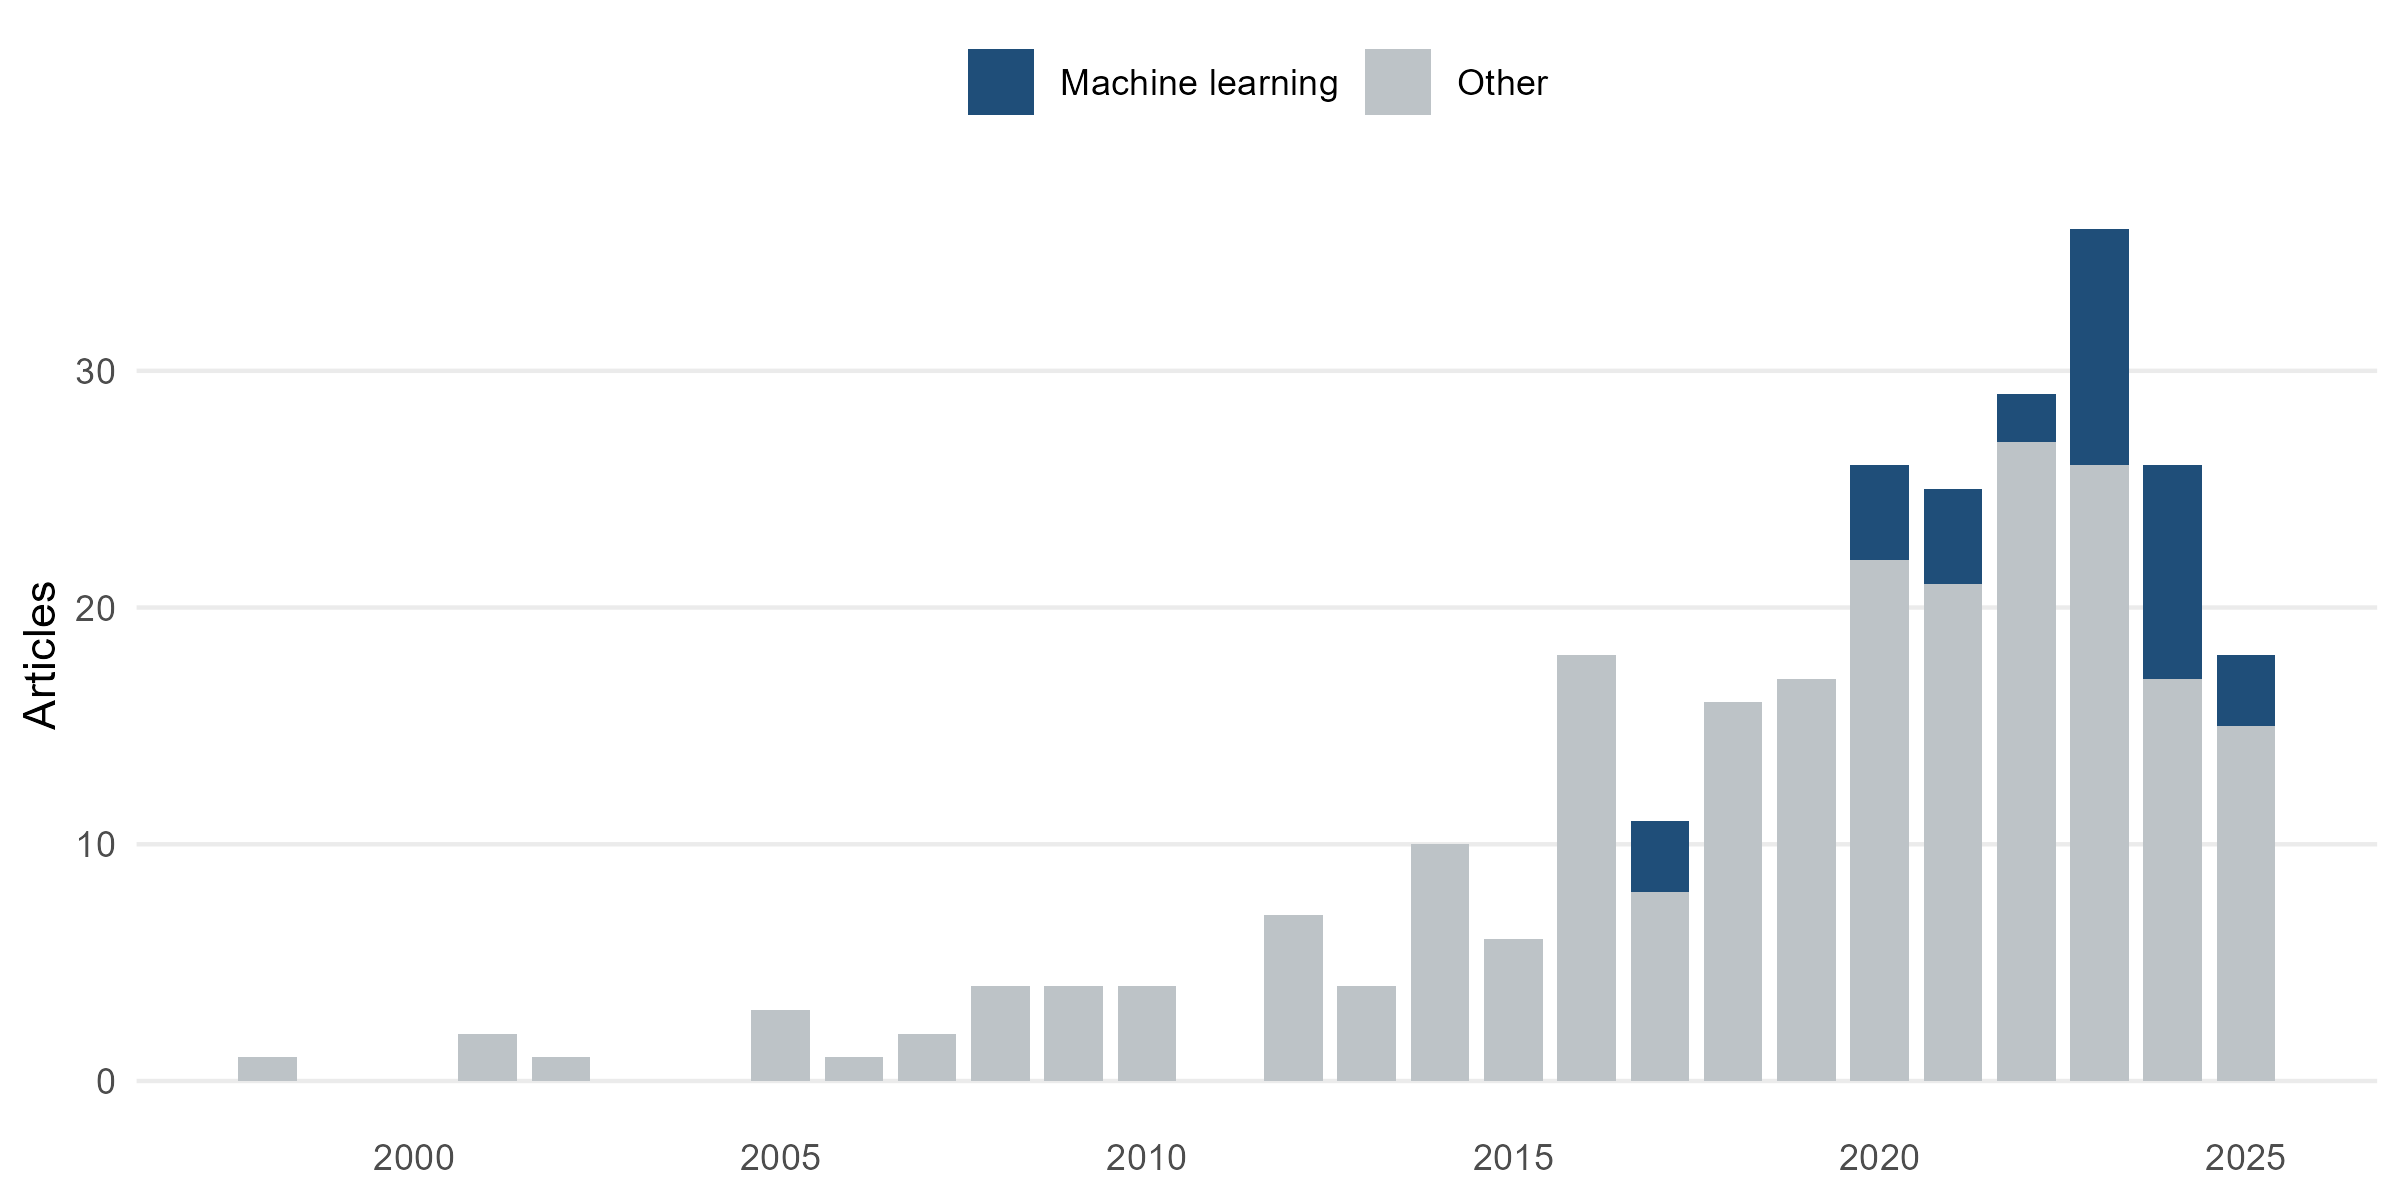
\includegraphics[width=\linewidth]{figures/literature_growth.png}
\label{fig:litgrowth}
\end{figure}


\begin{table}[pt]
\centering
\captionsetup{justification=raggedright,labelsep=none,singlelinecheck=false,labelformat=boldlabel}
\renewcommand{\arraystretch}{1.15}
\caption[The forecasting targets]{\footnotesize \textbf{: The forecasting targets.} Monthly realized variance, defined as the sum of squared daily returns within the month, in basis points. The market row is the value-weighted market portfolio. The factor row pools the 153 long-short factors, whose histories begin at different dates, so the panel is unbalanced and the pooled statistics weight each month by the number of factors available. Per-factor detail is in the Internet Appendix.}
\footnotesize
\setlength{\tabcolsep}{4pt}
\begin{tabularx}{\linewidth}{>{\raggedright\arraybackslash}X*{2}{>{\raggedleft\arraybackslash}m{1.5cm}}*{2}{>{\raggedleft\arraybackslash}m{0.9cm}}*{5}{>{\raggedleft\arraybackslash}m{1.1cm}}}
\hline
Target & Series & Obs. & From & To & Mean & S.D. & P10 & Median & P90 \\
\hline
Market & 1 & 1,188 & 1926 & 2024 & 25.28 & 52.09 & 3.84 & 10.50 & 51.70 \\
Factors, pooled & 153 & 146,439 & 1926 & 2025 & 7.06 & 21.93 & 0.49 & 1.89 & 13.48 \\
\hline
\end{tabularx}
\label{tab:sumtgt}
\end{table}


{\footnotesize
\captionsetup{justification=raggedright,labelsep=none,singlelinecheck=false,labelformat=boldlabel}
\setlength{\tabcolsep}{3pt}
\renewcommand{\arraystretch}{1.05}
\setlength{\emergencystretch}{3em}
\begin{longtable}{>{\raggedright\arraybackslash}m{4.7cm}>{\raggedleft\arraybackslash}m{0.8cm}>{\raggedleft\arraybackslash}m{0.8cm}*{5}{>{\raggedleft\arraybackslash}m{1.10cm}}}
\caption[Summary statistics for the predictors]{\footnotesize \textbf{: Summary statistics for the predictors.} Monthly observations of the market series, each variable measured over the longest window it supports. `From' is the first year available. Variance and quarticity measures are reported in basis points.} \label{tab:sumcov} \\
\hline
Predictor & Obs. & From & Mean & S.D. & P10 & Median & P90 \\
\hline
\endfirsthead
\hline
Predictor & Obs. & From & Mean & S.D. & P10 & Median & P90 \\
\hline
\endhead
\hline
\endfoot
Realized variance, daily term (bp) & 1176 & 1927 & 21.15 & 69.21 & 0.12 & 4.05 & 46.24 \\
Realized variance, weekly term (bp) & 1176 & 1927 & 24.11 & 72.57 & 2.23 & 9.00 & 53.05 \\
Realized variance, monthly term (bp) & 1176 & 1927 & 25.40 & 52.32 & 3.84 & 10.62 & 51.75 \\
Realized quarticity, daily term ($\times 10^{-8}$) & 1176 & 1927 & 79.29 & 780.97 & 0.00 & 0.25 & 32.40 \\
Realized quarticity, weekly term ($\times 10^{-8}$) & 1176 & 1927 & 32.49 & 529.09 & 0.03 & 0.55 & 17.57 \\
Realized quarticity, monthly term ($\times 10^{-8}$) & 1176 & 1927 & 8.53 & 69.12 & 0.03 & 0.25 & 5.93 \\
Jump variation, daily term (bp) & 1176 & 1927 & 7.02 & 30.97 & 0.00 & 0.00 & 13.41 \\
Jump variation, weekly term (bp) & 1176 & 1927 & 1.80 & 5.10 & 0.07 & 0.58 & 3.99 \\
Jump variation, monthly term (bp) & 1176 & 1927 & 0.44 & 1.04 & 0.06 & 0.18 & 0.94 \\
Continuous variation, daily term (bp) & 1176 & 1927 & 14.13 & 51.93 & 0.09 & 2.38 & 30.50 \\
Continuous variation, weekly term (bp) & 1176 & 1927 & 3.02 & 10.23 & 0.23 & 1.10 & 6.06 \\
Continuous variation, monthly term (bp) & 1176 & 1927 & 0.70 & 1.49 & 0.11 & 0.32 & 1.38 \\
Negative return, daily term & 1176 & 1927 & -0.06 & 0.13 & -0.18 & 0.00 & 0.00 \\
Negative return, weekly term & 1176 & 1927 & -0.03 & 0.06 & -0.10 & 0.00 & 0.00 \\
Negative return, monthly term & 1176 & 1927 & -0.01 & 0.03 & -0.05 & 0.00 & 0.00 \\
Policy uncertainty growth & 1176 & 1927 & 0.00 & 0.24 & -0.29 & -0.02 & 0.31 \\
Producer price volatility & 1176 & 1927 & 2.42 & 1.32 & 1.16 & 2.12 & 3.96 \\
Industrial production volatility & 1176 & 1927 & 5.61 & 2.94 & 2.98 & 4.84 & 9.18 \\
Monetary base volatility & 467 & 1986 & 3.42 & 4.27 & 0.86 & 1.39 & 8.56 \\
Dividend yield & 1176 & 1927 & 0.04 & 0.02 & 0.02 & 0.03 & 0.06 \\
Earnings yield & 1176 & 1927 & 0.07 & 0.03 & 0.04 & 0.06 & 0.11 \\
Default return spread & 467 & 1986 & 1.32 & 0.45 & 0.79 & 1.28 & 1.91 \\
Default yield spread & 467 & 1986 & 2.29 & 0.69 & 1.57 & 2.17 & 3.14 \\
Term spread & 467 & 1986 & 1.35 & 1.30 & -0.49 & 1.38 & 3.16 \\
Treasury bill rate & 467 & 1986 & 3.08 & 2.46 & 0.05 & 3.02 & 5.95 \\
Consumer sentiment growth & 467 & 1986 & -0.00 & 0.05 & -0.06 & -0.00 & 0.06 \\
Geopolitical risk & 1176 & 1927 & 0.00 & 0.22 & -0.24 & -0.01 & 0.24 \\
Crude oil variance, daily (bp) & 434 & 1986 & 218.09 & 1,636.80 & 0.94 & 28.21 & 279.69 \\
Crude oil variance, weekly (bp) & 467 & 1986 & 157.86 & 573.80 & 11.68 & 58.15 & 308.67 \\
Crude oil variance, monthly (bp) & 467 & 1986 & 144.70 & 372.64 & 27.03 & 74.16 & 233.72 \\
Implied volatility (bp) & 466 & 1986 & 37.87 & 35.57 & 12.85 & 27.94 & 68.31 \\
Trading days & 1176 & 1927 & 4.67 & 0.22 & 4.47 & 4.69 & 5.00 \\
\end{longtable}
}


\begin{figure}[htbp]
\centering
\captionsetup{justification=raggedright,labelsep=none,singlelinecheck=false,labelformat=boldlabel}
\caption[Monthly realized variance of the market and of the factor cross-section]{\footnotesize \textbf{: Monthly realized variance of the market and of the factor cross-section.} The dark line is the value-weighted market portfolio. The band is the 10th to 90th percentile of realized variance across the factors available in each month and the grey line is their median. The vertical scale is logarithmic.}
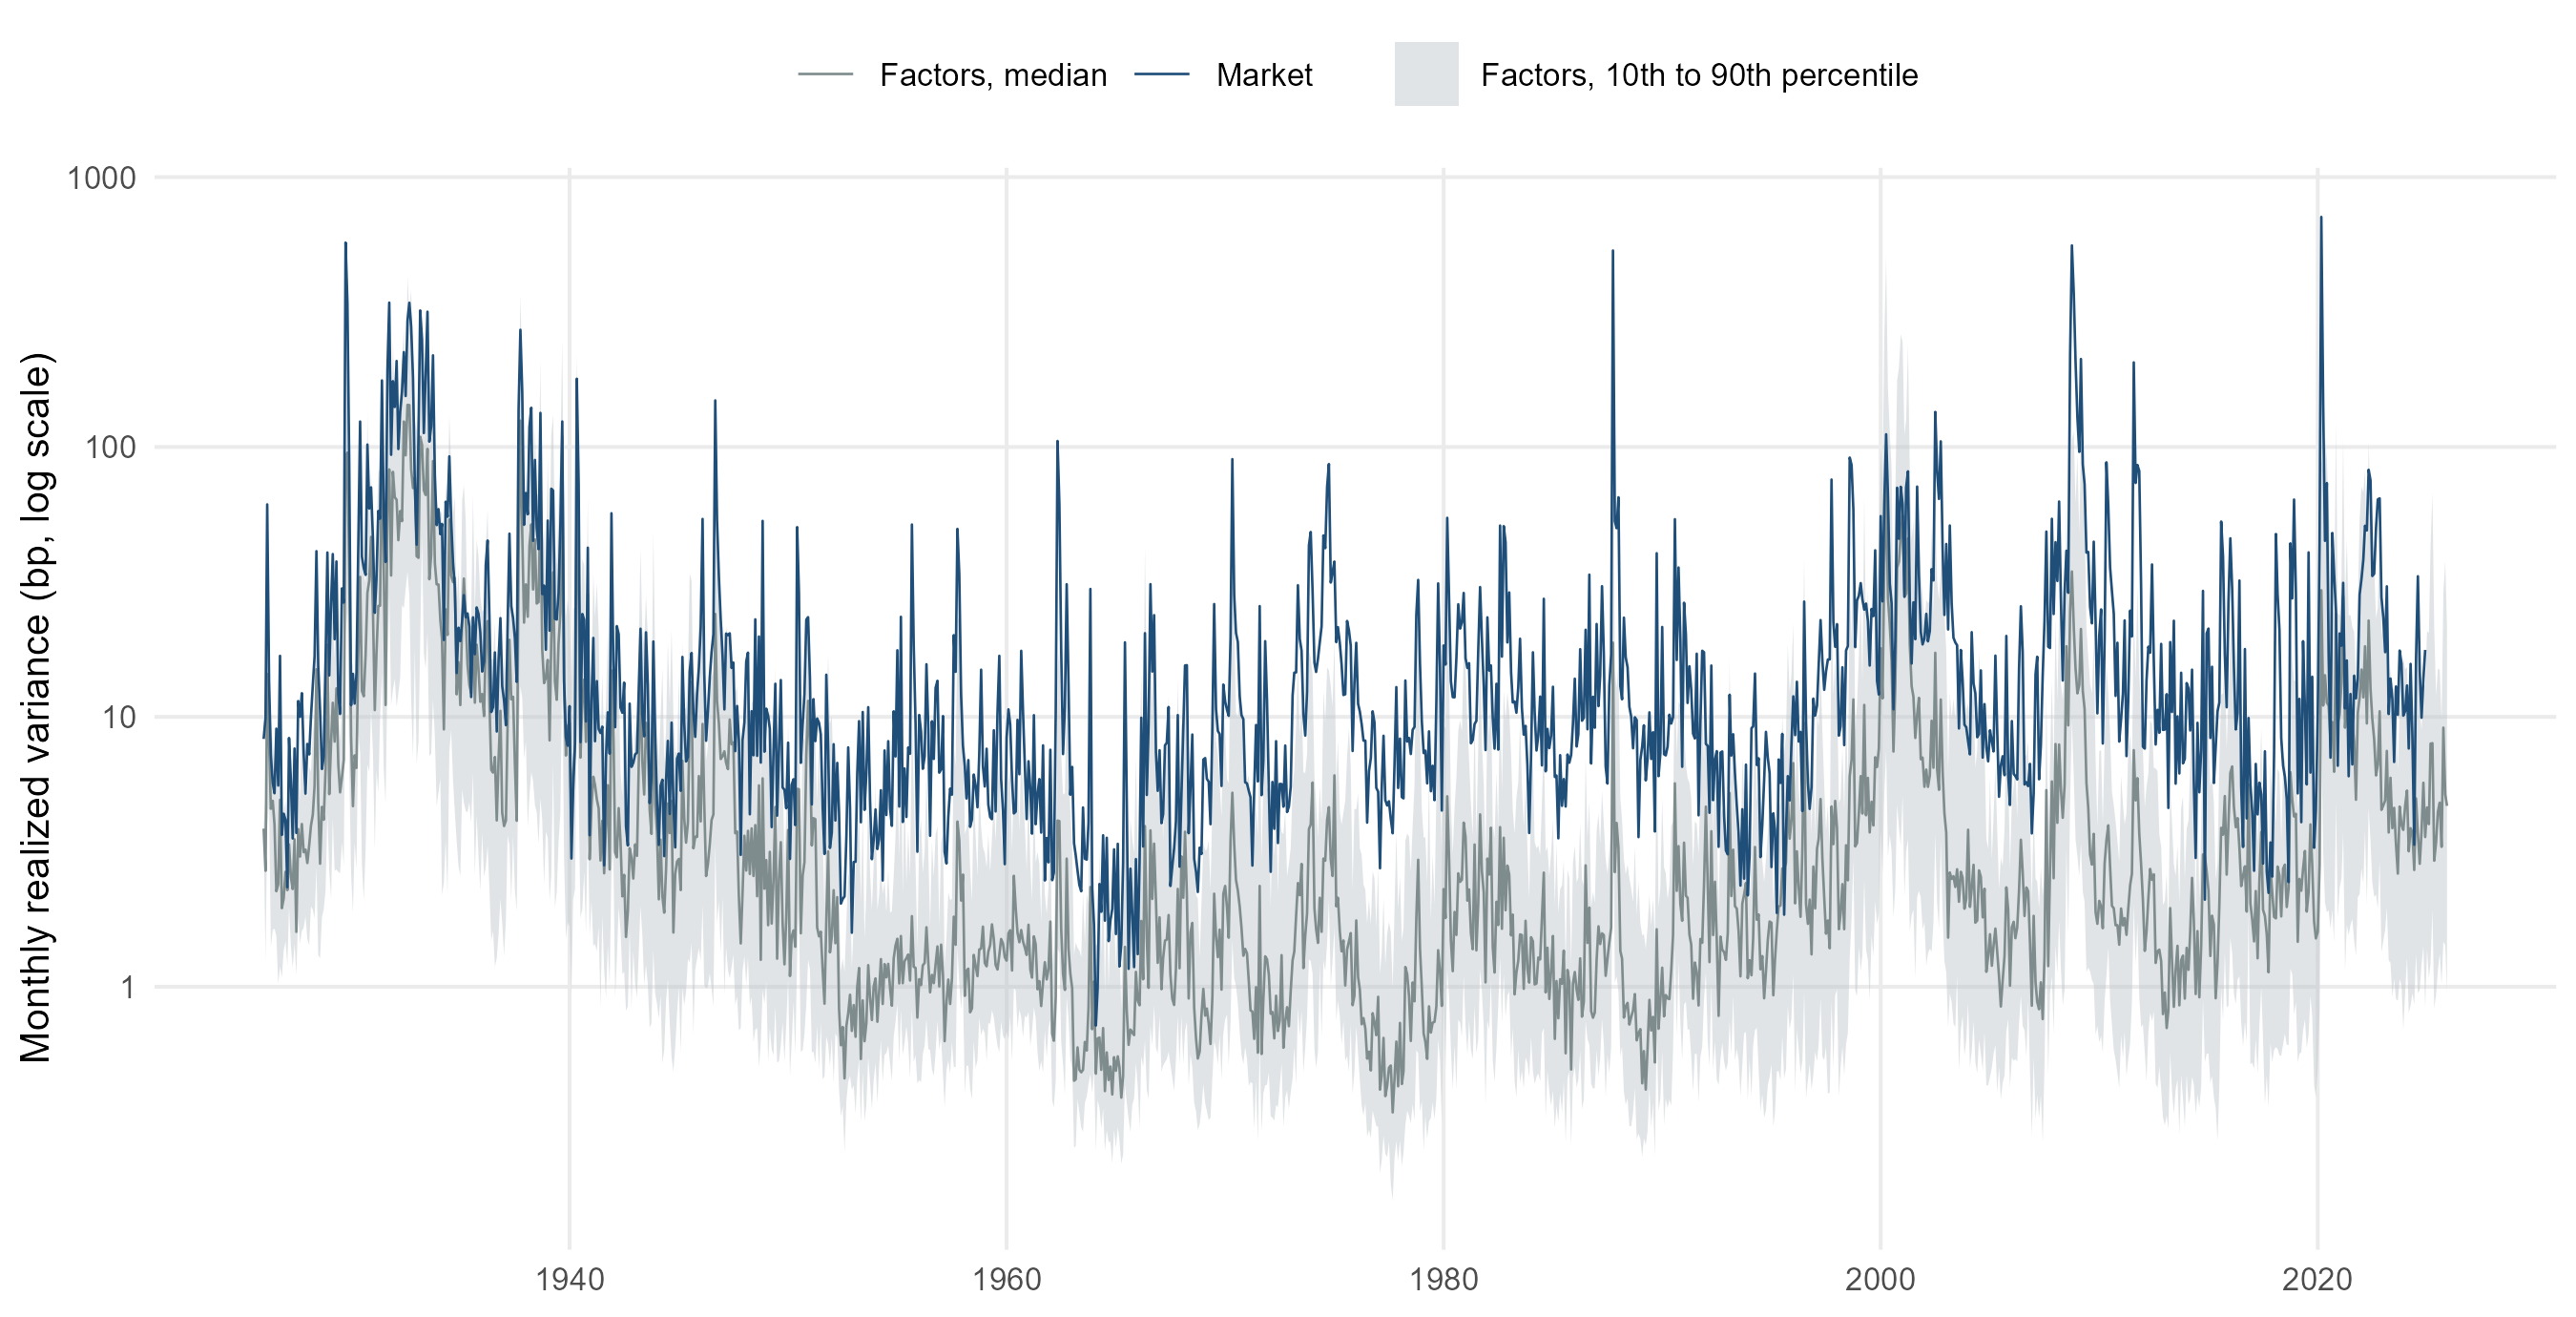
\includegraphics[width=\linewidth]{figures/data_targets.png}
\label{fig:targets}
\end{figure}


\begin{figure}[htbp]
\centering
\captionsetup{justification=raggedright,labelsep=none,singlelinecheck=false,labelformat=boldlabel}
\caption[Predictors over time]{\footnotesize \textbf{: Predictors over time.} Each panel plots one predictor for the market series over the longest window it supports, so panels start at different dates. Vertical scales are free. Variance and quarticity measures are in decimal units. The calendar month is omitted: it enters the models as twelve indicators and has no time-series interpretation.}
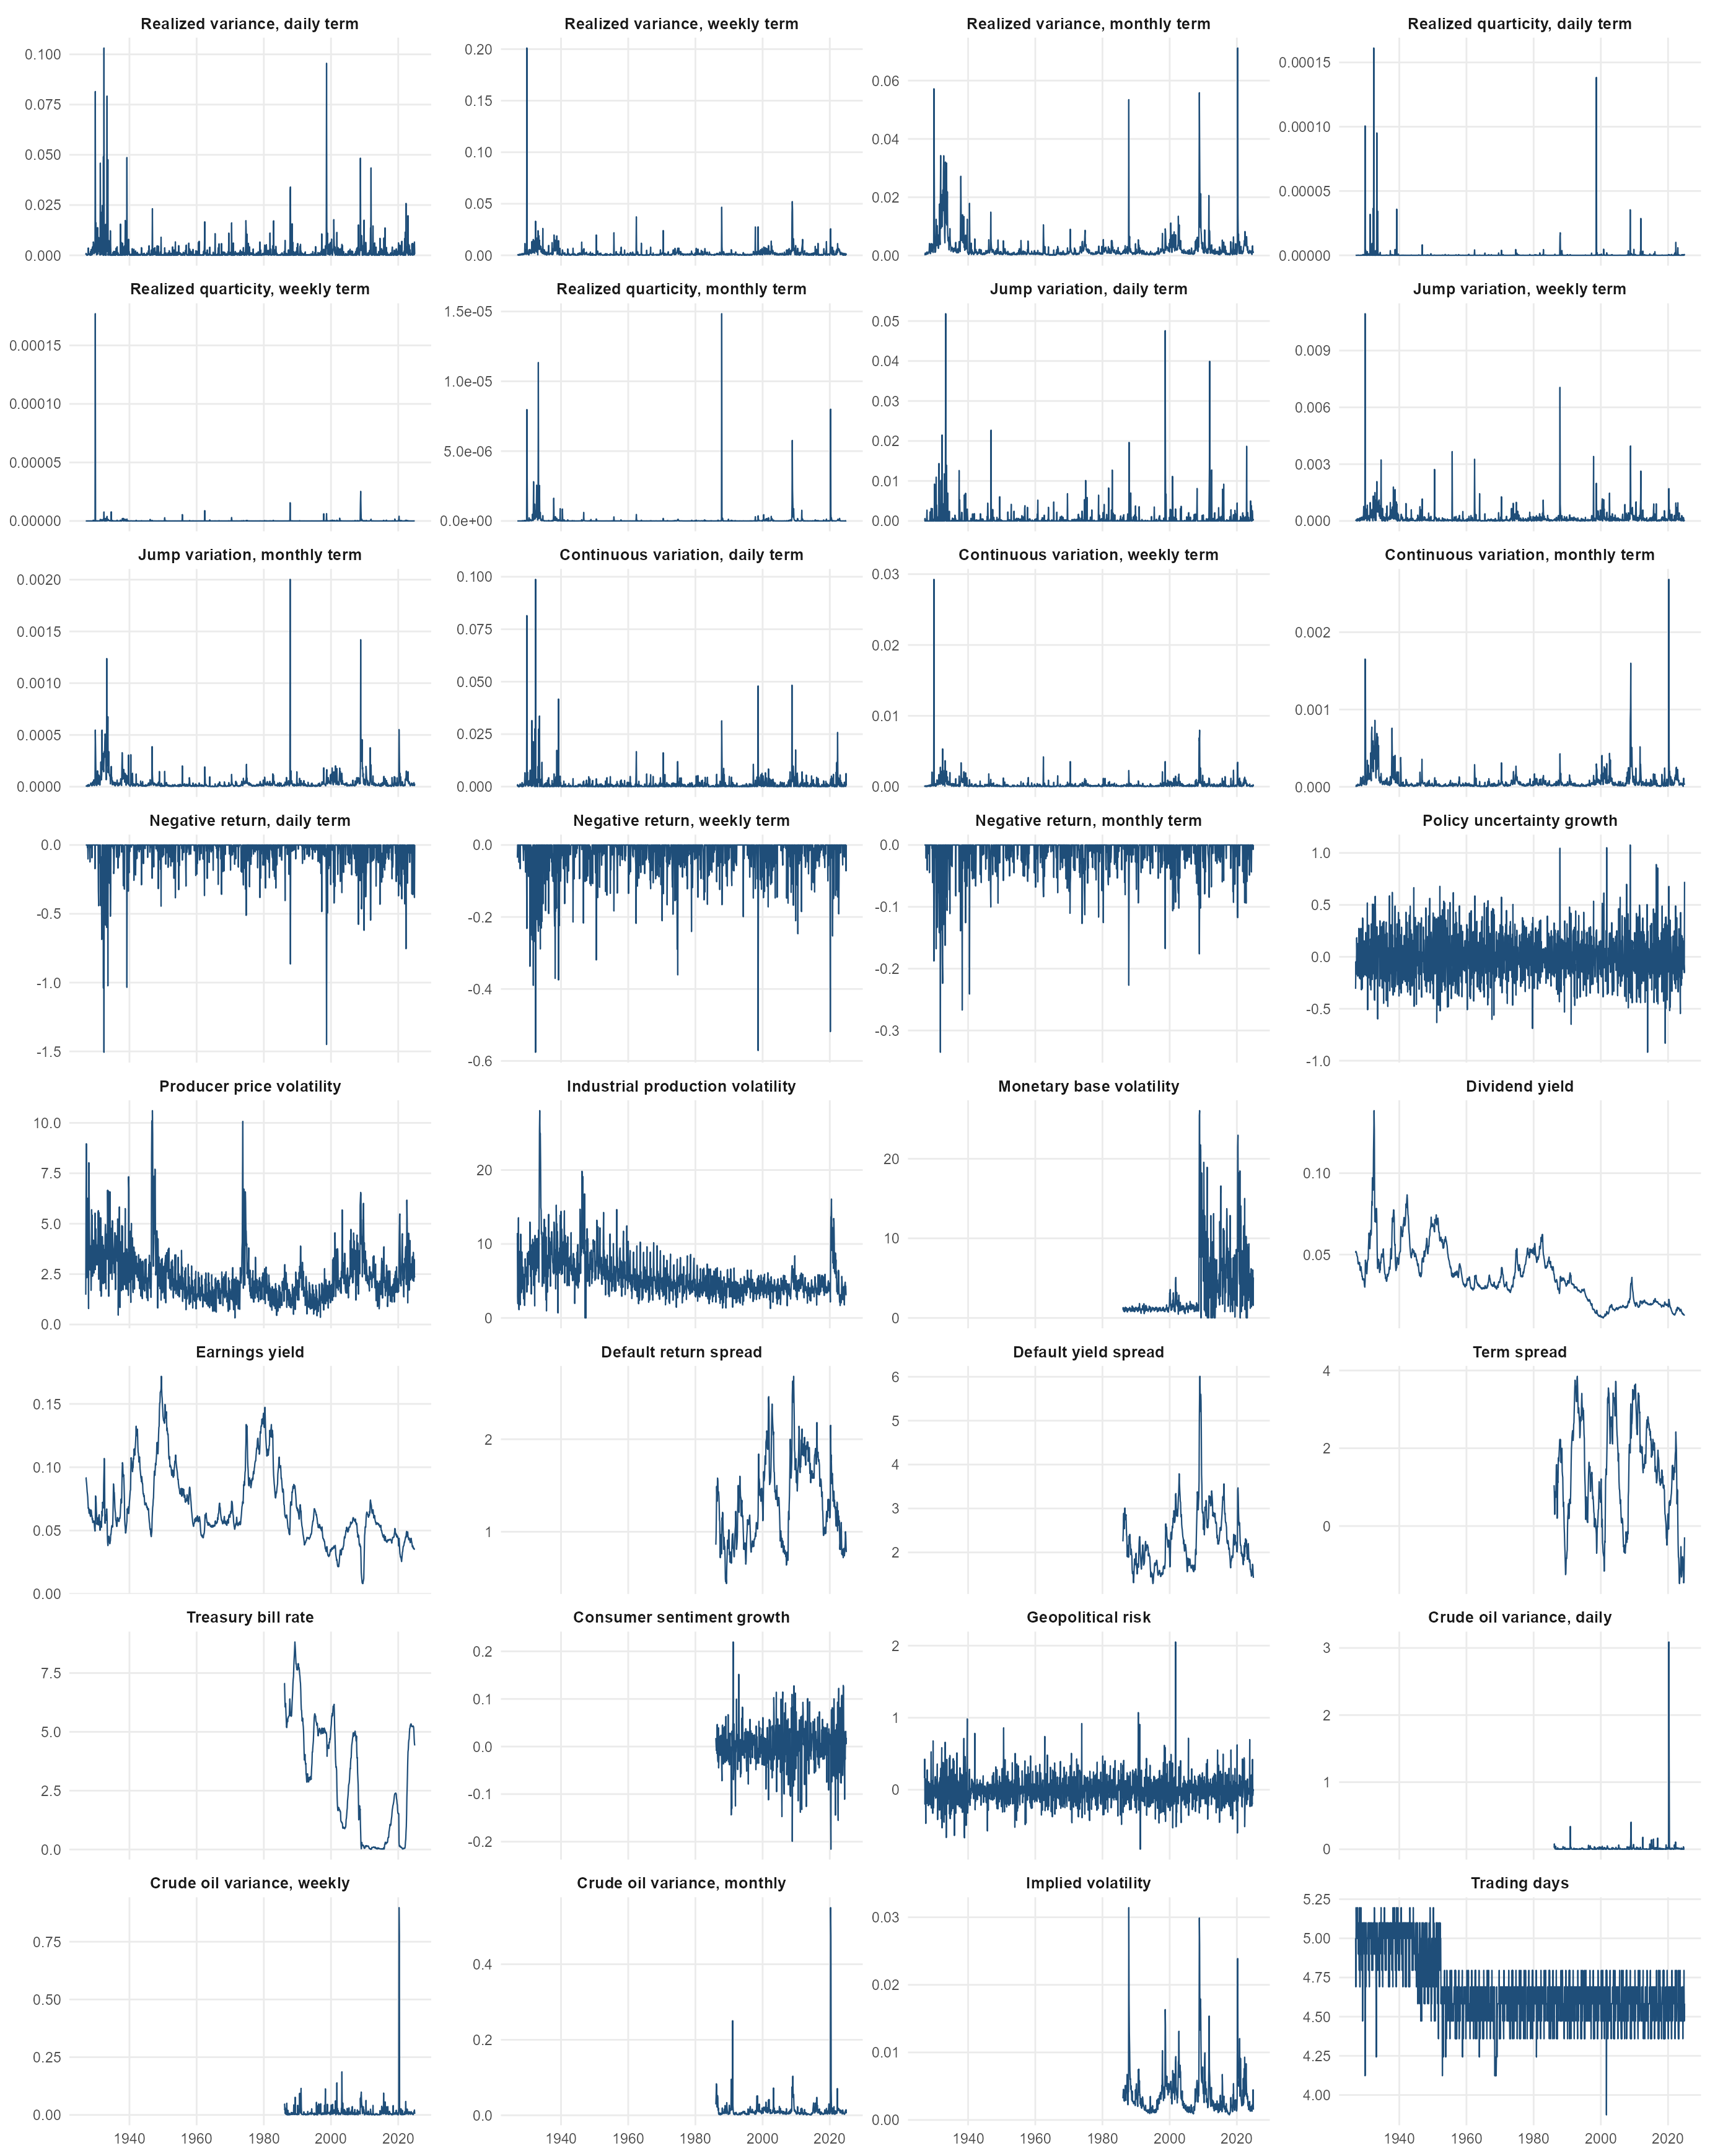
\includegraphics[width=\linewidth]{figures/data_covariates_grid.png}
\label{fig:covgrid}
\end{figure}


\clearpage

\subsection{Out-of-Sample Forecasting Results}

\begin{table}[p]
\centering\footnotesize
\captionsetup{justification=raggedright,labelsep=none,singlelinecheck=false,labelformat=boldlabel}
\renewcommand{\arraystretch}{0.88}\setlength{\tabcolsep}{4pt}
\caption[]{\footnotesize \textbf{: Out-of-sample predictive performance.} Statistics pool errors across the stated target-month observations. RMSE is Root Mean Squared Error. MAE is Mean Absolute Error. MPHE is mean pseudo-Huber error, MAPE is mean absolute percentage error and R-squared is the out-of-sample R² computed in relation to the target mean. Bias is realized minus predicted log variance. EW averages seven log forecasts, excluding HAR. Forecast evaluation spans June 1947 to December 2024 in the long sample and July 2006 to December 2024 in the short sample.}
\label{tab:rv-performance}
\resizebox{\ifdim\width>\linewidth\linewidth\else\width\fi}{!}{%
\begin{tabular}{lrrrrrr}
\multicolumn{7}{@{}l}{\textit{Panel A. Long sample: Pooled factor and market panel}} \\
\hline
Model & RMSE & MAE & MPHE & MAPE & R-squared & Bias \\
\hline
HAR & 0.7335 & 0.5602 & 0.2050 & 0.0721 & 0.6508 & 0.1147 \\
HARX & 0.7230 & 0.5509 & 0.1996 & 0.0710 & 0.6607 & 0.1266 \\
ENET & 0.7234 & 0.5513 & 0.1998 & 0.0711 & 0.6603 & 0.1081 \\
RF & 0.7201 & 0.5470 & 0.1976 & 0.0706 & 0.6634 & 0.1196 \\
XGB & 0.7420 & 0.5696 & 0.2098 & 0.0725 & 0.6426 & 0.0207 \\
NN1 & 0.7291 & 0.5557 & 0.2025 & 0.0717 & 0.6549 & 0.1331 \\
NN2 & 0.7188 & 0.5489 & 0.1978 & 0.0705 & 0.6646 & 0.0999 \\
NN3 & 0.7164 & 0.5483 & 0.1973 & 0.0704 & 0.6669 & 0.1105 \\
EW & 0.7076 & 0.5385 & 0.1922 & 0.0694 & 0.6750 & 0.1026 \\
\hline
\multicolumn{7}{@{}l}{\textit{Panel B. Long sample: Market portfolio from pooled estimation}} \\
\hline
Model & RMSE & MAE & MPHE & MAPE & R-squared & Bias \\
\hline
HAR & 0.8630 & 0.6677 & 0.2701 & 0.1102 & 0.1485 & 0.4904 \\
HARX & 0.8695 & 0.6835 & 0.2765 & 0.1121 & 0.1357 & 0.5070 \\
ENET & 0.8934 & 0.7040 & 0.2895 & 0.1156 & 0.0875 & 0.5416 \\
RF & 0.7708 & 0.5859 & 0.2215 & 0.0958 & 0.3207 & 0.3438 \\
XGB & 0.7987 & 0.6149 & 0.2358 & 0.1005 & 0.2707 & 0.3878 \\
NN1 & 0.8886 & 0.7028 & 0.2875 & 0.1145 & 0.0973 & 0.5393 \\
NN2 & 0.8489 & 0.6580 & 0.2635 & 0.1071 & 0.1761 & 0.4809 \\
NN3 & 0.8490 & 0.6592 & 0.2639 & 0.1073 & 0.1759 & 0.4891 \\
EW & 0.8336 & 0.6467 & 0.2555 & 0.1060 & 0.2056 & 0.4699 \\
\hline
\multicolumn{7}{@{}l}{\textit{Panel C. Short sample: Pooled factor and market panel}} \\
\hline
Model & RMSE & MAE & MPHE & MAPE & R-squared & Bias \\
\hline
HAR & 0.7287 & 0.5723 & 0.2079 & 0.0742 & 0.6743 & -0.1308 \\
HARX & 0.7267 & 0.5593 & 0.2033 & 0.0757 & 0.6761 & 0.1832 \\
ENET & 0.6990 & 0.5415 & 0.1915 & 0.0728 & 0.7003 & 0.0958 \\
RF & 0.6973 & 0.5452 & 0.1923 & 0.0722 & 0.7017 & 0.0214 \\
XGB & 0.7046 & 0.5512 & 0.1959 & 0.0724 & 0.6955 & -0.0296 \\
NN1 & 0.7246 & 0.5584 & 0.2028 & 0.0755 & 0.6779 & 0.1429 \\
NN2 & 0.7284 & 0.5627 & 0.2053 & 0.0758 & 0.6746 & 0.1108 \\
NN3 & 0.7267 & 0.5595 & 0.2035 & 0.0757 & 0.6760 & 0.1158 \\
EW & 0.6936 & 0.5352 & 0.1885 & 0.0719 & 0.7049 & 0.0915 \\
\hline
\multicolumn{7}{@{}l}{\textit{Panel D. Short sample: Market portfolio from pooled estimation}} \\
\hline
Model & RMSE & MAE & MPHE & MAPE & R-squared & Bias \\
\hline
HAR & 0.8205 & 0.6279 & 0.2459 & 0.1107 & 0.3643 & 0.1755 \\
HARX & 0.8246 & 0.6371 & 0.2482 & 0.1127 & 0.3580 & 0.2488 \\
ENET & 0.8254 & 0.6472 & 0.2520 & 0.1143 & 0.3566 & 0.2916 \\
RF & 0.8206 & 0.6346 & 0.2464 & 0.1127 & 0.3641 & 0.2195 \\
XGB & 0.8465 & 0.6512 & 0.2588 & 0.1157 & 0.3234 & 0.3353 \\
NN1 & 0.8600 & 0.6601 & 0.2645 & 0.1173 & 0.3017 & 0.2897 \\
NN2 & 0.8759 & 0.6704 & 0.2715 & 0.1195 & 0.2755 & 0.3411 \\
NN3 & 0.9040 & 0.6812 & 0.2829 & 0.1229 & 0.2283 & 0.3809 \\
EW & 0.8289 & 0.6321 & 0.2476 & 0.1130 & 0.3512 & 0.3010 \\
\hline
\end{tabular}}
\end{table}

\begin{table}[p]
\centering\scriptsize
\captionsetup{justification=raggedright,labelsep=none,singlelinecheck=false,labelformat=boldlabel}
\renewcommand{\arraystretch}{0.91}\setlength{\tabcolsep}{4pt}
\caption[]{\footnotesize \textbf{: Distribution of out-of-sample RMSE gains across the 153 equity factors.} Positive percentage gains indicate lower RMSE than HAR. Quantiles describe the cross-sectional distribution across factors. Forecast evaluation spans June 1947 to December 2024 in the long sample and July 2006 to December 2024 in the short sample.}
\label{tab:rv-factor_gain_summary}
\resizebox{\ifdim\width>\linewidth\linewidth\else\width\fi}{!}{%
\begin{tabular}{lrrrrr}
\multicolumn{6}{@{}l}{\textit{Panel A. Long sample}} \\
\hline
Model & Factors & Beating HAR & Median gain (\%) & P25 (\%) & P75 (\%) \\
\hline
HAR & 153 & 0 & 0.00 & 0.00 & 0.00 \\
HARX & 153 & 126 & 1.45 & 0.19 & 2.46 \\
ENET & 153 & 127 & 1.63 & 0.48 & 2.84 \\
RF & 153 & 92 & 1.46 & -1.49 & 4.10 \\
XGB & 153 & 58 & -2.30 & -5.62 & 2.41 \\
NN1 & 153 & 82 & 0.20 & -1.40 & 2.05 \\
NN2 & 153 & 111 & 1.80 & -0.10 & 3.42 \\
NN3 & 153 & 118 & 2.02 & 0.20 & 3.87 \\
EW & 153 & 145 & 3.24 & 2.11 & 4.95 \\
\hline
\multicolumn{6}{@{}l}{\textit{Panel B. Short sample}} \\
\hline
Model & Factors & Beating HAR & Median gain (\%) & P25 (\%) & P75 (\%) \\
\hline
HAR & 153 & 0 & 0.00 & 0.00 & 0.00 \\
HARX & 153 & 74 & -0.57 & -5.65 & 6.82 \\
ENET & 153 & 107 & 3.49 & -0.93 & 8.63 \\
RF & 153 & 112 & 4.49 & -0.63 & 7.80 \\
XGB & 153 & 101 & 3.19 & -1.68 & 7.35 \\
NN1 & 153 & 76 & -0.09 & -5.57 & 6.63 \\
NN2 & 153 & 69 & -0.92 & -6.89 & 5.83 \\
NN3 & 153 & 77 & 0.28 & -6.44 & 6.32 \\
EW & 153 & 110 & 4.00 & -0.56 & 10.46 \\
\hline
\end{tabular}}
\end{table}

\begin{figure}[p]
\centering
\captionsetup{justification=raggedright,labelsep=none,singlelinecheck=false,labelformat=boldlabel}
\caption[]{\footnotesize \textbf{: Out-of-sample RMSE gains relative to HAR.} Dots identify the long sample and crosses the short sample. Each comparison uses that sample's HAR. Panel statistics pool squared errors across target-month observations before taking the square root.}
\label{fig:rv-har_relative_gains}
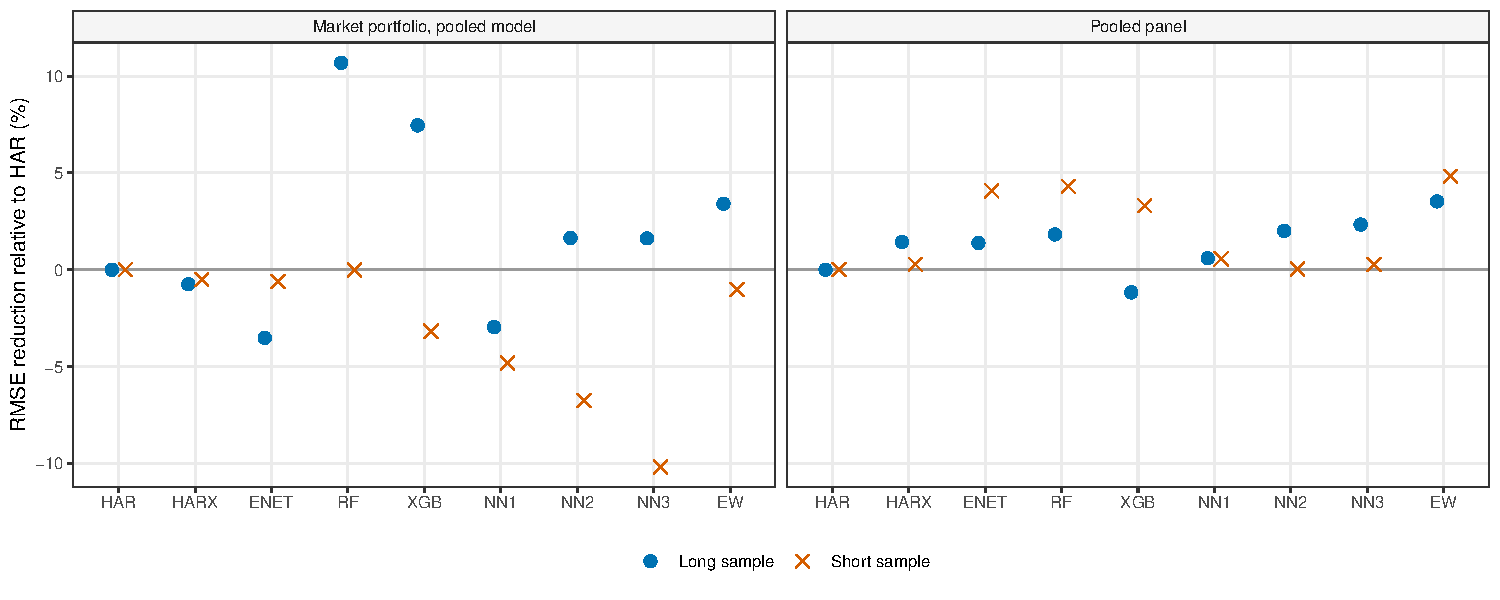
\includegraphics[width=\linewidth,height=0.70\textheight,keepaspectratio]{results_v3/combined/main/har_relative_gains.pdf}
\end{figure}

\begin{table}[p]
\centering\scriptsize
\captionsetup{justification=raggedright,labelsep=none,singlelinecheck=false,labelformat=boldlabel}
\renewcommand{\arraystretch}{0.91}\setlength{\tabcolsep}{4pt}
\caption[]{\footnotesize \textbf{: Economic performance of volatility-managed portfolios.} Raw and capped columns report gross performance. Net columns deduct 10 basis points per unit change in factor exposure. The cap is 1.5. CER uses risk aversion five. The factor aggregate equal-weights 153 nonmarket factors within each month. Long-sample market strategies span June 1952 to December 2024 and factor aggregates January 1980 to December 2024. Short-sample strategies span July 2011 to December 2024.}
\label{tab:rv-portfolio_performance}
\resizebox{\ifdim\width>\linewidth\linewidth\else\width\fi}{!}{%
\begin{tabular}{lrrrrr}
\multicolumn{6}{@{}l}{\textit{Panel A. Long sample: Market portfolio, pooled estimation}} \\
\hline
Model & Statistic & Raw & Capped & Net raw & Net capped \\
\hline
Unmanaged & Sharpe ratio & 0.499 & 0.499 & 0.499 & 0.499 \\
Unmanaged & CER (\%) & 1.842 & 1.842 & 1.841 & 1.841 \\
Unmanaged & Volatility ratio & 1.000 & 1.000 & 1.000 & 1.000 \\
Unmanaged & Mean raw exposure & 1.000 & 1.000 & 1.000 & 1.000 \\
Random walk & Sharpe ratio & 0.507 & 0.539 & 0.463 & 0.514 \\
Random walk & CER (\%) & -0.385 & 2.752 & -1.280 & 2.424 \\
Random walk & Volatility ratio & 1.392 & 0.877 & 1.389 & 0.877 \\
Random walk & Mean raw exposure & 1.503 & 1.503 & 1.503 & 1.503 \\
HAR & Sharpe ratio & 0.549 & 0.545 & 0.523 & 0.522 \\
HAR & CER (\%) & 2.932 & 2.921 & 2.592 & 2.635 \\
HAR & Volatility ratio & 0.851 & 0.820 & 0.851 & 0.820 \\
HAR & Mean raw exposure & 0.970 & 0.970 & 0.970 & 0.970 \\
HARX & Sharpe ratio & 0.550 & 0.550 & 0.524 & 0.528 \\
HARX & CER (\%) & 2.952 & 2.981 & 2.612 & 2.702 \\
HARX & Volatility ratio & 0.847 & 0.820 & 0.847 & 0.820 \\
HARX & Mean raw exposure & 0.957 & 0.957 & 0.957 & 0.957 \\
EW & Sharpe ratio & 0.551 & 0.543 & 0.523 & 0.520 \\
EW & CER (\%) & 2.989 & 2.918 & 2.654 & 2.637 \\
EW & Volatility ratio & 0.815 & 0.795 & 0.815 & 0.795 \\
EW & Mean raw exposure & 0.926 & 0.926 & 0.926 & 0.926 \\
\hline
\multicolumn{6}{@{}l}{\textit{Panel B. Long sample: Equal-weighted factor panel}} \\
\hline
Model & Statistic & Raw & Capped & Net raw & Net capped \\
\hline
Unmanaged & Sharpe ratio & 0.718 & 0.718 & 0.718 & 0.718 \\
Unmanaged & CER (\%) & 2.274 & 2.274 & 2.274 & 2.274 \\
Unmanaged & Volatility ratio & 1.000 & 1.000 & 1.000 & 1.000 \\
Unmanaged & Mean raw exposure & 1.000 & 1.000 & 1.000 & 1.000 \\
Random walk & Sharpe ratio & 1.027 & 1.053 & 0.731 & 0.831 \\
Random walk & CER (\%) & 1.834 & 1.471 & 1.270 & 1.149 \\
Random walk & Volatility ratio & 0.516 & 0.399 & 0.512 & 0.399 \\
Random walk & Mean raw exposure & 0.909 & 0.909 & 0.909 & 0.909 \\
HAR & Sharpe ratio & 0.996 & 0.995 & 0.798 & 0.833 \\
HAR & CER (\%) & 1.704 & 1.616 & 1.348 & 1.341 \\
HAR & Volatility ratio & 0.494 & 0.468 & 0.494 & 0.468 \\
HAR & Mean raw exposure & 0.838 & 0.838 & 0.838 & 0.838 \\
HARX & Sharpe ratio & 1.019 & 1.023 & 0.825 & 0.861 \\
HARX & CER (\%) & 1.687 & 1.616 & 1.348 & 1.348 \\
HARX & Volatility ratio & 0.477 & 0.455 & 0.476 & 0.454 \\
HARX & Mean raw exposure & 0.807 & 0.807 & 0.807 & 0.807 \\
EW & Sharpe ratio & 1.071 & 1.076 & 0.887 & 0.920 \\
EW & CER (\%) & 1.789 & 1.710 & 1.466 & 1.452 \\
EW & Volatility ratio & 0.481 & 0.456 & 0.479 & 0.456 \\
EW & Mean raw exposure & 0.854 & 0.854 & 0.854 & 0.854 \\
\hline
\end{tabular}}
\end{table}
\begin{table}[p]
\ContinuedFloat
\centering\scriptsize
\captionsetup{justification=raggedright,labelsep=none,singlelinecheck=false,labelformat=boldlabel}
\renewcommand{\arraystretch}{0.91}\setlength{\tabcolsep}{4pt}
\caption[]{\footnotesize \textbf{: Economic performance of volatility-managed portfolios. Continued.} Short-sample results. Definitions and conventions follow the preceding panels.}
\resizebox{\ifdim\width>\linewidth\linewidth\else\width\fi}{!}{%
\begin{tabular}{lrrrrr}
\multicolumn{6}{@{}l}{\textit{Panel C. Short sample: Market portfolio, pooled estimation}} \\
\hline
Model & Statistic & Raw & Capped & Net raw & Net capped \\
\hline
Unmanaged & Sharpe ratio & 0.770 & 0.770 & 0.769 & 0.769 \\
Unmanaged & CER (\%) & 5.922 & 5.922 & 5.913 & 5.913 \\
Unmanaged & Volatility ratio & 1.000 & 1.000 & 1.000 & 1.000 \\
Unmanaged & Mean raw exposure & 1.000 & 1.000 & 1.000 & 1.000 \\
Random walk & Sharpe ratio & 0.554 & 0.737 & 0.498 & 0.692 \\
Random walk & CER (\%) & 2.518 & 4.963 & 1.630 & 4.492 \\
Random walk & Volatility ratio & 1.053 & 0.695 & 1.054 & 0.695 \\
Random walk & Mean raw exposure & 1.080 & 1.080 & 1.080 & 1.080 \\
HAR & Sharpe ratio & 0.733 & 0.847 & 0.691 & 0.828 \\
HAR & CER (\%) & 4.583 & 7.002 & 3.727 & 6.732 \\
HAR & Volatility ratio & 1.353 & 0.958 & 1.353 & 0.958 \\
HAR & Mean raw exposure & 1.612 & 1.612 & 1.612 & 1.612 \\
HARX & Sharpe ratio & 0.761 & 0.752 & 0.721 & 0.731 \\
HARX & CER (\%) & 5.605 & 5.632 & 4.889 & 5.342 \\
HARX & Volatility ratio & 1.199 & 0.936 & 1.197 & 0.937 \\
HARX & Mean raw exposure & 1.471 & 1.471 & 1.471 & 1.471 \\
EW & Sharpe ratio & 0.766 & 0.778 & 0.731 & 0.760 \\
EW & CER (\%) & 5.729 & 6.024 & 5.112 & 5.760 \\
EW & Volatility ratio & 1.176 & 0.970 & 1.176 & 0.971 \\
EW & Mean raw exposure & 1.460 & 1.460 & 1.460 & 1.460 \\
\hline
\multicolumn{6}{@{}l}{\textit{Panel D. Short sample: Equal-weighted factor panel}} \\
\hline
Model & Statistic & Raw & Capped & Net raw & Net capped \\
\hline
Unmanaged & Sharpe ratio & 0.483 & 0.483 & 0.480 & 0.480 \\
Unmanaged & CER (\%) & 1.115 & 1.115 & 1.108 & 1.108 \\
Unmanaged & Volatility ratio & 1.000 & 1.000 & 1.001 & 1.001 \\
Unmanaged & Mean raw exposure & 1.000 & 1.000 & 1.000 & 1.000 \\
Random walk & Sharpe ratio & 0.640 & 0.597 & 0.330 & 0.371 \\
Random walk & CER (\%) & 1.005 & 0.759 & 0.481 & 0.453 \\
Random walk & Volatility ratio & 0.626 & 0.502 & 0.622 & 0.501 \\
Random walk & Mean raw exposure & 0.852 & 0.852 & 0.852 & 0.852 \\
HAR & Sharpe ratio & 0.644 & 0.601 & 0.428 & 0.465 \\
HAR & CER (\%) & 1.357 & 1.120 & 0.857 & 0.844 \\
HAR & Volatility ratio & 0.863 & 0.759 & 0.862 & 0.760 \\
HAR & Mean raw exposure & 1.161 & 1.161 & 1.161 & 1.161 \\
HARX & Sharpe ratio & 0.611 & 0.631 & 0.403 & 0.501 \\
HARX & CER (\%) & 1.279 & 1.179 & 0.797 & 0.916 \\
HARX & Volatility ratio & 0.862 & 0.757 & 0.860 & 0.757 \\
HARX & Mean raw exposure & 1.136 & 1.136 & 1.136 & 1.136 \\
EW & Sharpe ratio & 0.643 & 0.641 & 0.468 & 0.523 \\
EW & CER (\%) & 1.331 & 1.199 & 0.932 & 0.959 \\
EW & Volatility ratio & 0.846 & 0.756 & 0.845 & 0.756 \\
EW & Mean raw exposure & 1.132 & 1.132 & 1.132 & 1.132 \\
\hline
\end{tabular}}
\end{table}

\begin{table}[p]
\centering\scriptsize
\captionsetup{justification=raggedright,labelsep=none,singlelinecheck=false,labelformat=boldlabel}
\renewcommand{\arraystretch}{0.91}\setlength{\tabcolsep}{4pt}
\caption[]{\footnotesize \textbf{: Economic performance of fixed 50/50 unmanaged and volatility-managed combinations.} Each managed row combines equal unmanaged and own-variance-managed sleeves. Total factor exposure is bounded by five. Returns, volatility, CER and costs are annualized percentages. Turnover is the monthly absolute exposure change. EW denotes the forecast ensemble. Long-sample market strategies span June 1952 to December 2024 and factor aggregates January 1980 to December 2024. Short-sample strategies span July 2011 to December 2024.}
\label{tab:rv-portfolio_performance_cederburg_ew}
\resizebox{\ifdim\width>\linewidth\linewidth\else\width\fi}{!}{%
\begin{tabular}{lrrrrrrr}
\multicolumn{8}{@{}l}{\textit{Panel A. Long sample: Market portfolio, pooled estimation}} \\
\hline
Model & Return (\%) & Vol. (\%) & Gross SR & Net SR & CER (\%) & Turnover & Cost (\%) \\
\hline
Unmanaged & 7.530 & 15.086 & 0.499 & 0.499 & 1.841 & 0.001 & 0.001 \\
Random walk & 8.525 & 16.430 & 0.547 & 0.519 & 1.776 & 0.383 & 0.460 \\
HAR & 7.119 & 13.530 & 0.539 & 0.526 & 2.543 & 0.143 & 0.172 \\
HARX & 7.112 & 13.484 & 0.540 & 0.527 & 2.567 & 0.143 & 0.172 \\
EW forecast ensemble & 6.982 & 13.218 & 0.541 & 0.528 & 2.614 & 0.141 & 0.170 \\
\hline
\multicolumn{8}{@{}l}{\textit{Panel B. Long sample: Equal-weighted 153-factor aggregate}} \\
\hline
Model & Return (\%) & Vol. (\%) & Gross SR & Net SR & CER (\%) & Turnover & Cost (\%) \\
\hline
Unmanaged & 2.602 & 3.623 & 0.718 & 0.718 & 2.274 & 0.000 & 0.000 \\
Random walk & 1.980 & 2.418 & 0.934 & 0.819 & 1.833 & 0.235 & 0.282 \\
HAR & 2.015 & 2.571 & 0.853 & 0.784 & 1.850 & 0.148 & 0.178 \\
HARX & 2.012 & 2.551 & 0.855 & 0.789 & 1.850 & 0.141 & 0.169 \\
EW forecast ensemble & 2.072 & 2.537 & 0.880 & 0.817 & 1.911 & 0.135 & 0.162 \\
\hline
\multicolumn{8}{@{}l}{\textit{Panel C. Short sample: Market portfolio, pooled estimation}} \\
\hline
Model & Return (\%) & Vol. (\%) & Gross SR & Net SR & CER (\%) & Turnover & Cost (\%) \\
\hline
Unmanaged & 11.527 & 14.985 & 0.770 & 0.769 & 5.913 & 0.006 & 0.007 \\
Random walk & 9.697 & 13.803 & 0.735 & 0.702 & 4.934 & 0.367 & 0.440 \\
HAR & 12.766 & 16.623 & 0.794 & 0.768 & 5.858 & 0.356 & 0.428 \\
HARX & 12.232 & 15.577 & 0.809 & 0.785 & 6.166 & 0.308 & 0.370 \\
EW forecast ensemble & 12.199 & 15.529 & 0.806 & 0.786 & 6.170 & 0.260 & 0.312 \\
\hline
\multicolumn{8}{@{}l}{\textit{Panel D. Short sample: Equal-weighted 153-factor aggregate}} \\
\hline
Model & Return (\%) & Vol. (\%) & Gross SR & Net SR & CER (\%) & Turnover & Cost (\%) \\
\hline
Unmanaged & 1.288 & 2.686 & 0.483 & 0.480 & 1.108 & 0.006 & 0.007 \\
Random walk & 0.920 & 1.990 & 0.595 & 0.462 & 0.821 & 0.222 & 0.266 \\
HAR & 1.140 & 2.393 & 0.582 & 0.476 & 0.996 & 0.211 & 0.254 \\
HARX & 1.109 & 2.380 & 0.569 & 0.466 & 0.968 & 0.204 & 0.245 \\
EW forecast ensemble & 1.174 & 2.362 & 0.583 & 0.497 & 1.035 & 0.170 & 0.204 \\
\hline
\end{tabular}}
\end{table}

\begin{table}[p]
\centering\scriptsize
\captionsetup{justification=raggedright,labelsep=none,singlelinecheck=false,labelformat=boldlabel}
\renewcommand{\arraystretch}{0.91}\setlength{\tabcolsep}{4pt}
\caption[]{\footnotesize \textbf{: Economic performance of multifactor volatility-managed portfolios.} UMV holds 154 unmanaged factors. CMV conditions on market volatility and FCMV on each factor's own volatility. EW and HEW identify allocation rules. EW in a forecast row denotes the forecast ensemble. Exposure is capped at 1.5. Returns, volatility, CER and costs are annualized percentages. Long-sample evaluation spans January 1980 to December 2024. Short-sample evaluation spans July 2011 to December 2024.}
\label{tab:rv-portfolio_performance_multifactor}
\resizebox{\ifdim\width>\linewidth\linewidth\else\width\fi}{!}{%
\begin{tabular}{lrrrrrrr}
\multicolumn{8}{@{}l}{\textit{Panel A. Long sample: Equal-weight allocation}} \\
\hline
Model & Return (\%) & Vol. (\%) & Gross SR & Net SR & CER (\%) & Turnover & Cost (\%) \\
\hline
UMV & 2.637 & 3.543 & 0.745 & 0.744 & 2.323 & 0.002 & 0.002 \\
CMV, lagged market RV & 2.503 & 3.103 & 0.864 & 0.807 & 2.263 & 0.146 & 0.176 \\
CMV, HAR & 2.562 & 3.275 & 0.813 & 0.782 & 2.293 & 0.082 & 0.099 \\
CMV, HARX & 2.524 & 3.226 & 0.812 & 0.782 & 2.264 & 0.079 & 0.094 \\
CMV, EW forecast ensemble & 2.510 & 3.176 & 0.822 & 0.790 & 2.258 & 0.084 & 0.100 \\
FCMV, HAR & 2.370 & 3.020 & 0.822 & 0.785 & 2.142 & 0.093 & 0.111 \\
FCMV, HARX & 2.383 & 3.018 & 0.826 & 0.789 & 2.155 & 0.091 & 0.109 \\
FCMV, EW forecast ensemble & 2.394 & 2.978 & 0.838 & 0.804 & 2.173 & 0.083 & 0.100 \\
\hline
\multicolumn{8}{@{}l}{\textit{Panel B. Long sample: Hierarchical equal-weight allocation}} \\
\hline
Model & Return (\%) & Vol. (\%) & Gross SR & Net SR & CER (\%) & Turnover & Cost (\%) \\
\hline
UMV & 2.819 & 1.808 & 1.560 & 1.560 & 2.738 & 0.002 & 0.002 \\
CMV, lagged market RV & 2.676 & 1.634 & 1.745 & 1.637 & 2.609 & 0.145 & 0.175 \\
CMV, HAR & 2.725 & 1.704 & 1.657 & 1.600 & 2.653 & 0.082 & 0.098 \\
CMV, HARX & 2.678 & 1.679 & 1.651 & 1.595 & 2.608 & 0.078 & 0.094 \\
CMV, EW forecast ensemble & 2.672 & 1.654 & 1.676 & 1.616 & 2.604 & 0.083 & 0.100 \\
FCMV, HAR & 2.584 & 1.556 & 1.732 & 1.661 & 2.524 & 0.092 & 0.111 \\
FCMV, HARX & 2.580 & 1.551 & 1.733 & 1.663 & 2.520 & 0.090 & 0.108 \\
FCMV, EW forecast ensemble & 2.596 & 1.536 & 1.755 & 1.690 & 2.537 & 0.083 & 0.100 \\
\hline
\multicolumn{8}{@{}l}{\textit{Panel C. Short sample: Equal-weight allocation}} \\
\hline
Model & Return (\%) & Vol. (\%) & Gross SR & Net SR & CER (\%) & Turnover & Cost (\%) \\
\hline
UMV & 1.355 & 2.621 & 0.520 & 0.517 & 1.183 & 0.006 & 0.007 \\
CMV, lagged market RV & 1.290 & 2.602 & 0.586 & 0.496 & 1.120 & 0.192 & 0.231 \\
CMV, HAR & 1.328 & 2.671 & 0.561 & 0.497 & 1.149 & 0.140 & 0.168 \\
CMV, HARX & 1.325 & 2.622 & 0.567 & 0.506 & 1.154 & 0.134 & 0.161 \\
CMV, EW forecast ensemble & 1.355 & 2.621 & 0.570 & 0.517 & 1.183 & 0.115 & 0.138 \\
FCMV, HAR & 1.317 & 2.500 & 0.580 & 0.527 & 1.161 & 0.110 & 0.132 \\
FCMV, HARX & 1.326 & 2.503 & 0.582 & 0.530 & 1.169 & 0.109 & 0.131 \\
FCMV, EW forecast ensemble & 1.348 & 2.483 & 0.588 & 0.543 & 1.194 & 0.092 & 0.110 \\
\hline
\multicolumn{8}{@{}l}{\textit{Panel D. Short sample: Hierarchical equal-weight allocation}} \\
\hline
Model & Return (\%) & Vol. (\%) & Gross SR & Net SR & CER (\%) & Turnover & Cost (\%) \\
\hline
UMV & 1.835 & 1.406 & 1.314 & 1.305 & 1.785 & 0.006 & 0.007 \\
CMV, lagged market RV & 1.886 & 1.528 & 1.393 & 1.234 & 1.827 & 0.192 & 0.231 \\
CMV, HAR & 1.890 & 1.517 & 1.363 & 1.246 & 1.832 & 0.141 & 0.169 \\
CMV, HARX & 1.878 & 1.478 & 1.383 & 1.270 & 1.824 & 0.134 & 0.161 \\
CMV, EW forecast ensemble & 1.895 & 1.476 & 1.381 & 1.284 & 1.841 & 0.115 & 0.138 \\
FCMV, HAR & 1.854 & 1.409 & 1.418 & 1.316 & 1.804 & 0.115 & 0.138 \\
FCMV, HARX & 1.850 & 1.393 & 1.428 & 1.328 & 1.801 & 0.113 & 0.135 \\
FCMV, EW forecast ensemble & 1.869 & 1.388 & 1.431 & 1.346 & 1.820 & 0.094 & 0.113 \\
\hline
\end{tabular}}
\end{table}



\clearpage

\subsection{Additional Forecasting Results}

\begin{figure}[p]
\centering
\captionsetup{justification=raggedright,labelsep=none,singlelinecheck=false,labelformat=boldlabel}
\caption[]{\footnotesize \textbf{: Predictor-theme absolute loading shares at the final model refit.} Panel A reports the long sample and Panel B the short sample. Columns distinguish pooled and separate market estimation. Linear surrogate coefficients are normalized by the sum of absolute non-intercept coefficients before aggregation by theme. Blank cells indicate absent loadings. These descriptive associations are not causal importance measures.}
\label{fig:rv-final_theme_gross_share}
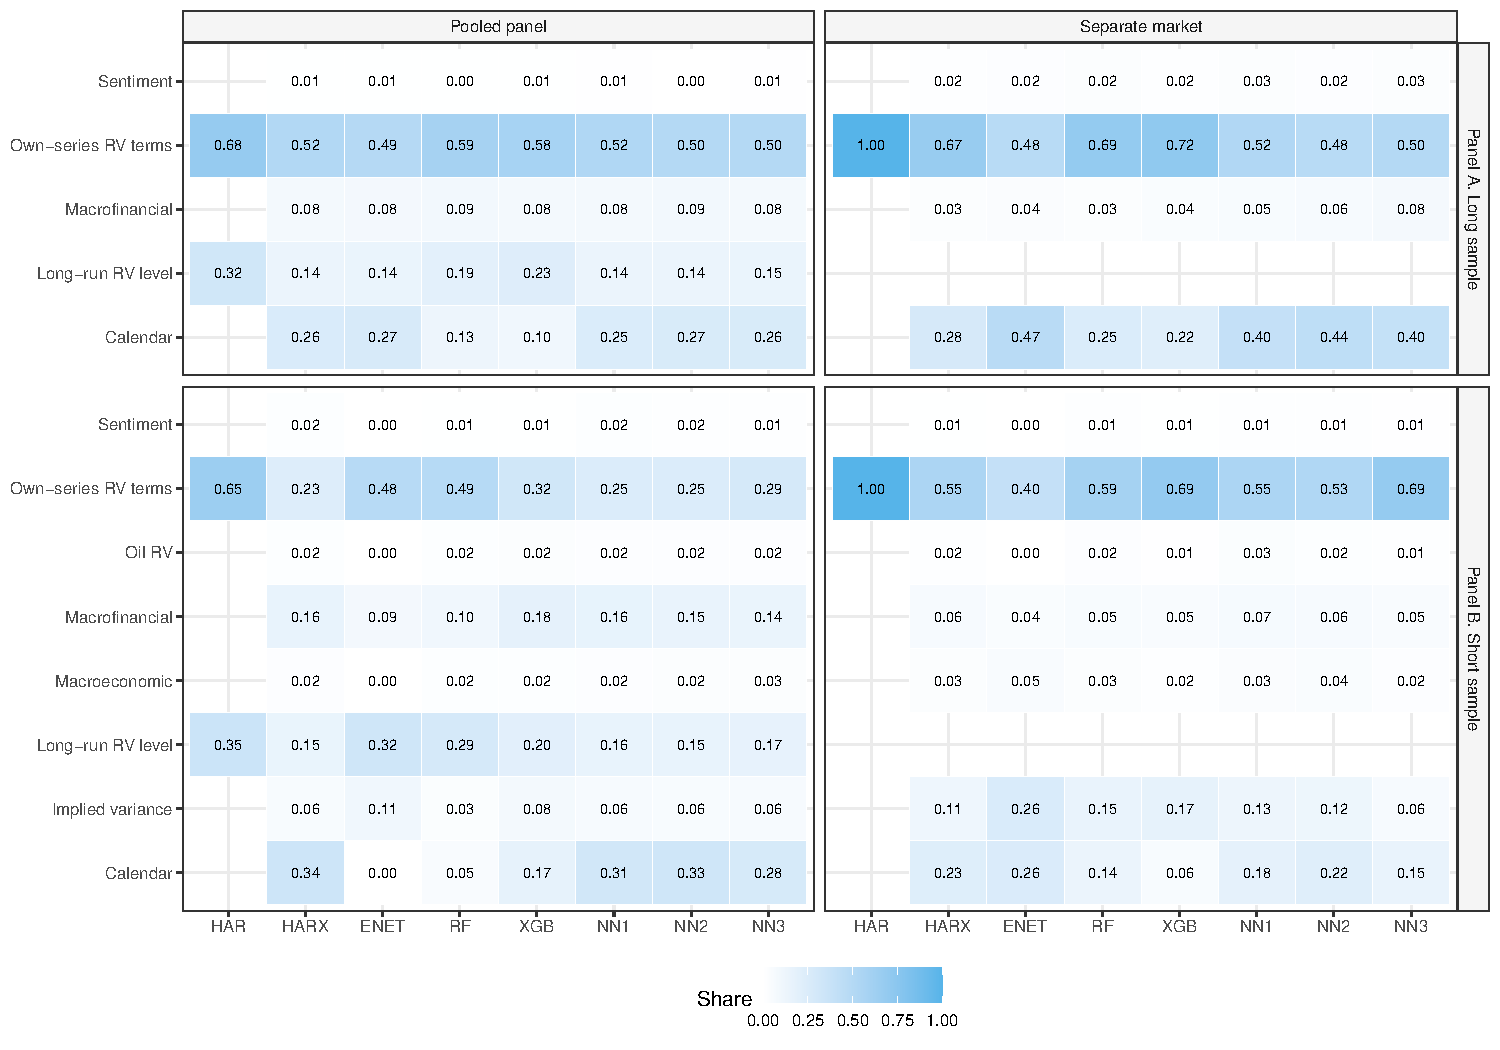
\includegraphics[width=\linewidth,height=0.70\textheight,keepaspectratio]{results_v3/combined/main_appendix/final_theme_gross_share.pdf}
\end{figure}

\begin{figure}[p]
\centering
\captionsetup{justification=raggedright,labelsep=none,singlelinecheck=false,labelformat=boldlabel}
\caption[]{\footnotesize \textbf{: Gross and net Sharpe ratios for the market portfolio using pooled forecasts.} Panel A reports the long sample and Panel B the short sample. Pale bars are gross and solid bars are net of modeled factor-exposure costs. EW denotes the forecast ensemble. Each construction retains its stated exposure cap. }
\label{fig:rv-portfolio_wealth_market_pooled}
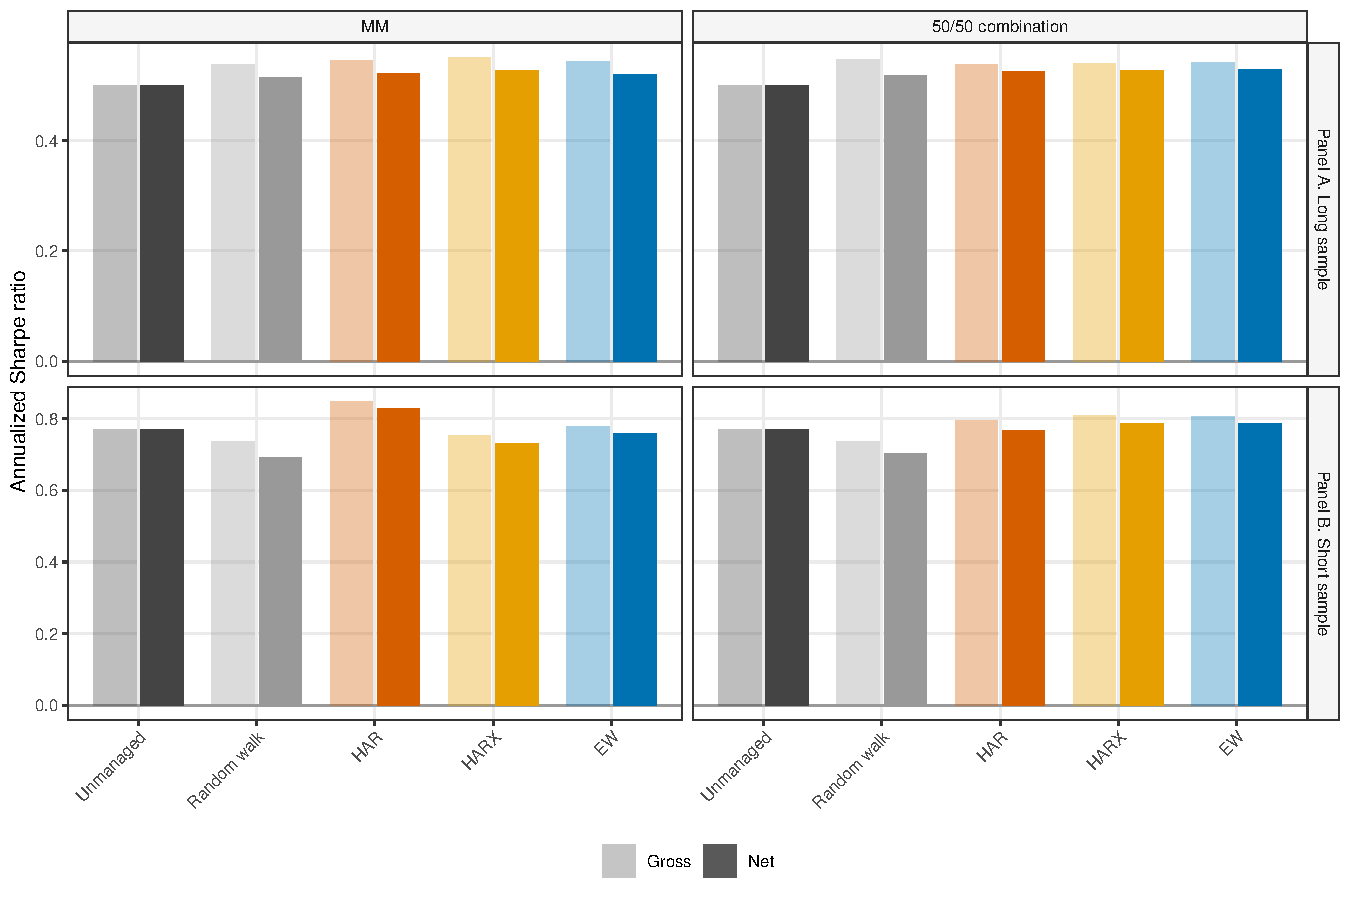
\includegraphics[width=\linewidth,height=0.70\textheight,keepaspectratio]{results_v3/combined/main_appendix/portfolio_wealth_market_pooled.pdf}
\end{figure}

\begin{figure}[p]
\centering
\captionsetup{justification=raggedright,labelsep=none,singlelinecheck=false,labelformat=boldlabel}
\caption[]{\footnotesize \textbf{: Gross and net Sharpe ratios for factor aggregates and multifactor allocations.} Panel A reports the long sample and Panel B the short sample. Pale bars are gross and solid bars are net of modeled factor-exposure costs. EW denotes the forecast ensemble. Each construction retains its stated exposure cap. MM and 50/50 combinations equal-weight the 153 nonmarket factors. Multifactor allocations include the market. In CMV, Random walk denotes the lagged-market signal. FCMV comparisons use HAR, HARX and the ensemble. Unmanaged denotes the matching UMV in multifactor panels.}
\label{fig:rv-portfolio_wealth_factor_panel}
\par\smallskip\textbf{Panel A. Long sample}\par\smallskip
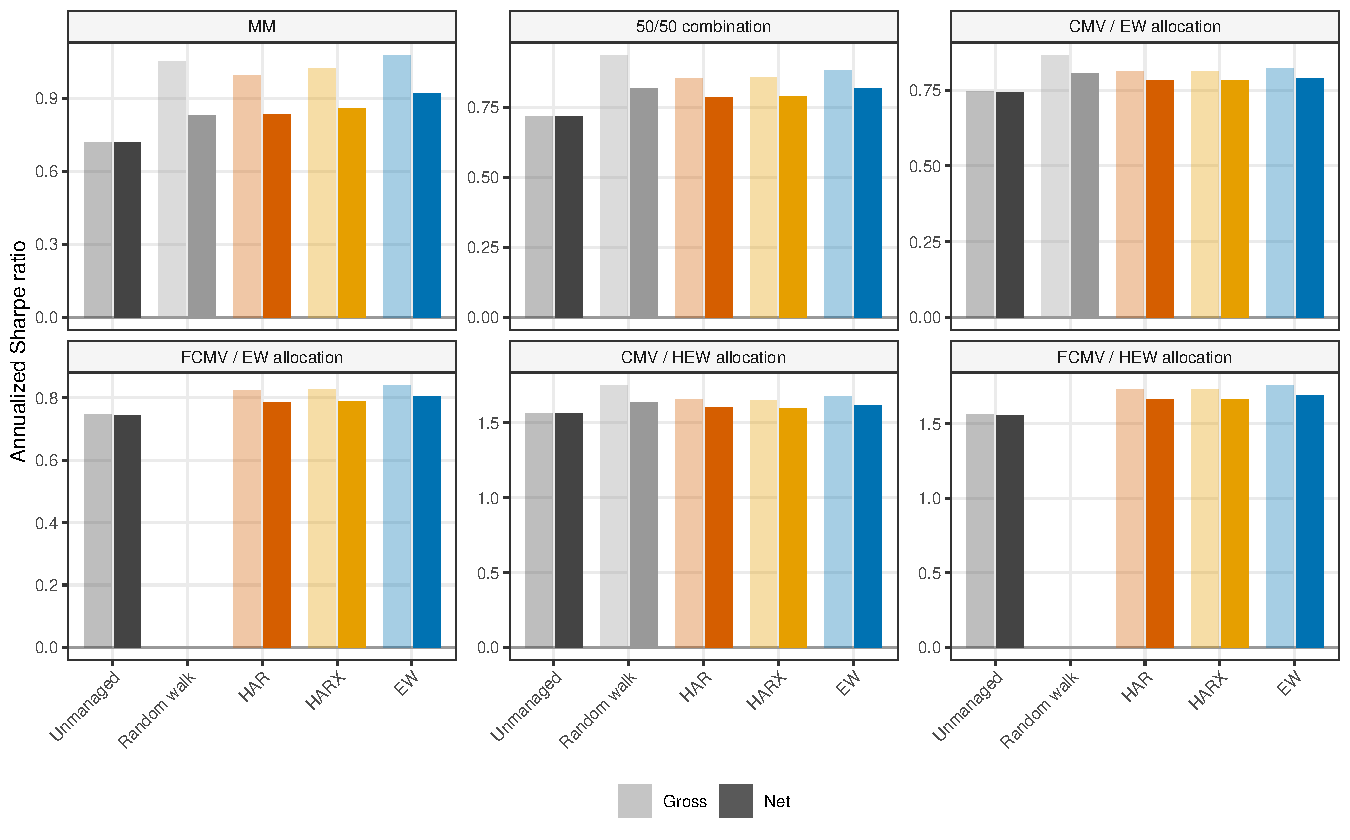
\includegraphics[width=\linewidth,height=0.70\textheight,keepaspectratio]{results_v3/combined/main_appendix/portfolio_wealth_factor_panel_1.pdf}
\end{figure}
\begin{figure}[p]
\ContinuedFloat
\centering
\captionsetup{justification=raggedright,labelsep=none,singlelinecheck=false,labelformat=boldlabel}
\caption[]{\footnotesize \textbf{: Gross and net Sharpe ratios for factor aggregates and multifactor allocations.} Panel A reports the long sample and Panel B the short sample. Pale bars are gross and solid bars are net of modeled factor-exposure costs. EW denotes the forecast ensemble. Each construction retains its stated exposure cap. MM and 50/50 combinations equal-weight the 153 nonmarket factors. Multifactor allocations include the market. In CMV, Random walk denotes the lagged-market signal. FCMV comparisons use HAR, HARX and the ensemble. Unmanaged denotes the matching UMV in multifactor panels. Continued.}
\par\smallskip\textbf{Panel B. Short sample}\par\smallskip
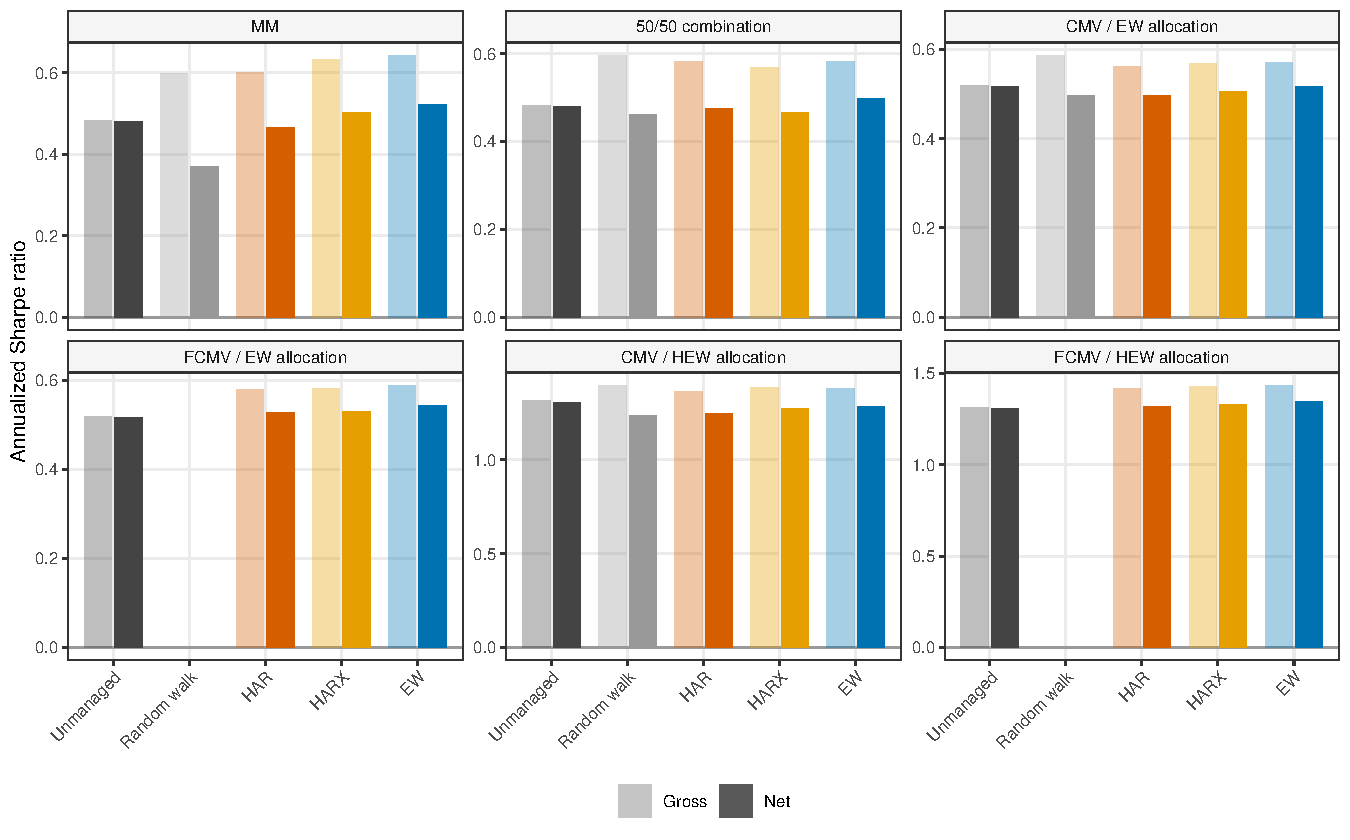
\includegraphics[width=\linewidth,height=0.70\textheight,keepaspectratio]{results_v3/combined/main_appendix/portfolio_wealth_factor_panel_2.pdf}
\end{figure}

\begin{figure}[p]
\centering
\captionsetup{justification=raggedright,labelsep=none,singlelinecheck=false,labelformat=boldlabel}
\caption[]{\footnotesize \textbf{: Cross-sectional distribution of net Sharpe ratios for volatility-managed factor portfolios by Jensen, Kelly, and Pedersen factor cluster.} Each box summarizes the factor-level Sharpe ratios within the indicated cluster. The center line is the median, the box spans the interquartile range, and the whiskers extend to the most extreme observations within 1.5 interquartile ranges. Managed strategies cap exposure at 1.5 and deduct 10 basis points per unit change in factor exposure.}
\label{fig:rv-portfolio_cluster_sharpe}
\par\smallskip\textbf{Panel A. Long sample}\par\smallskip
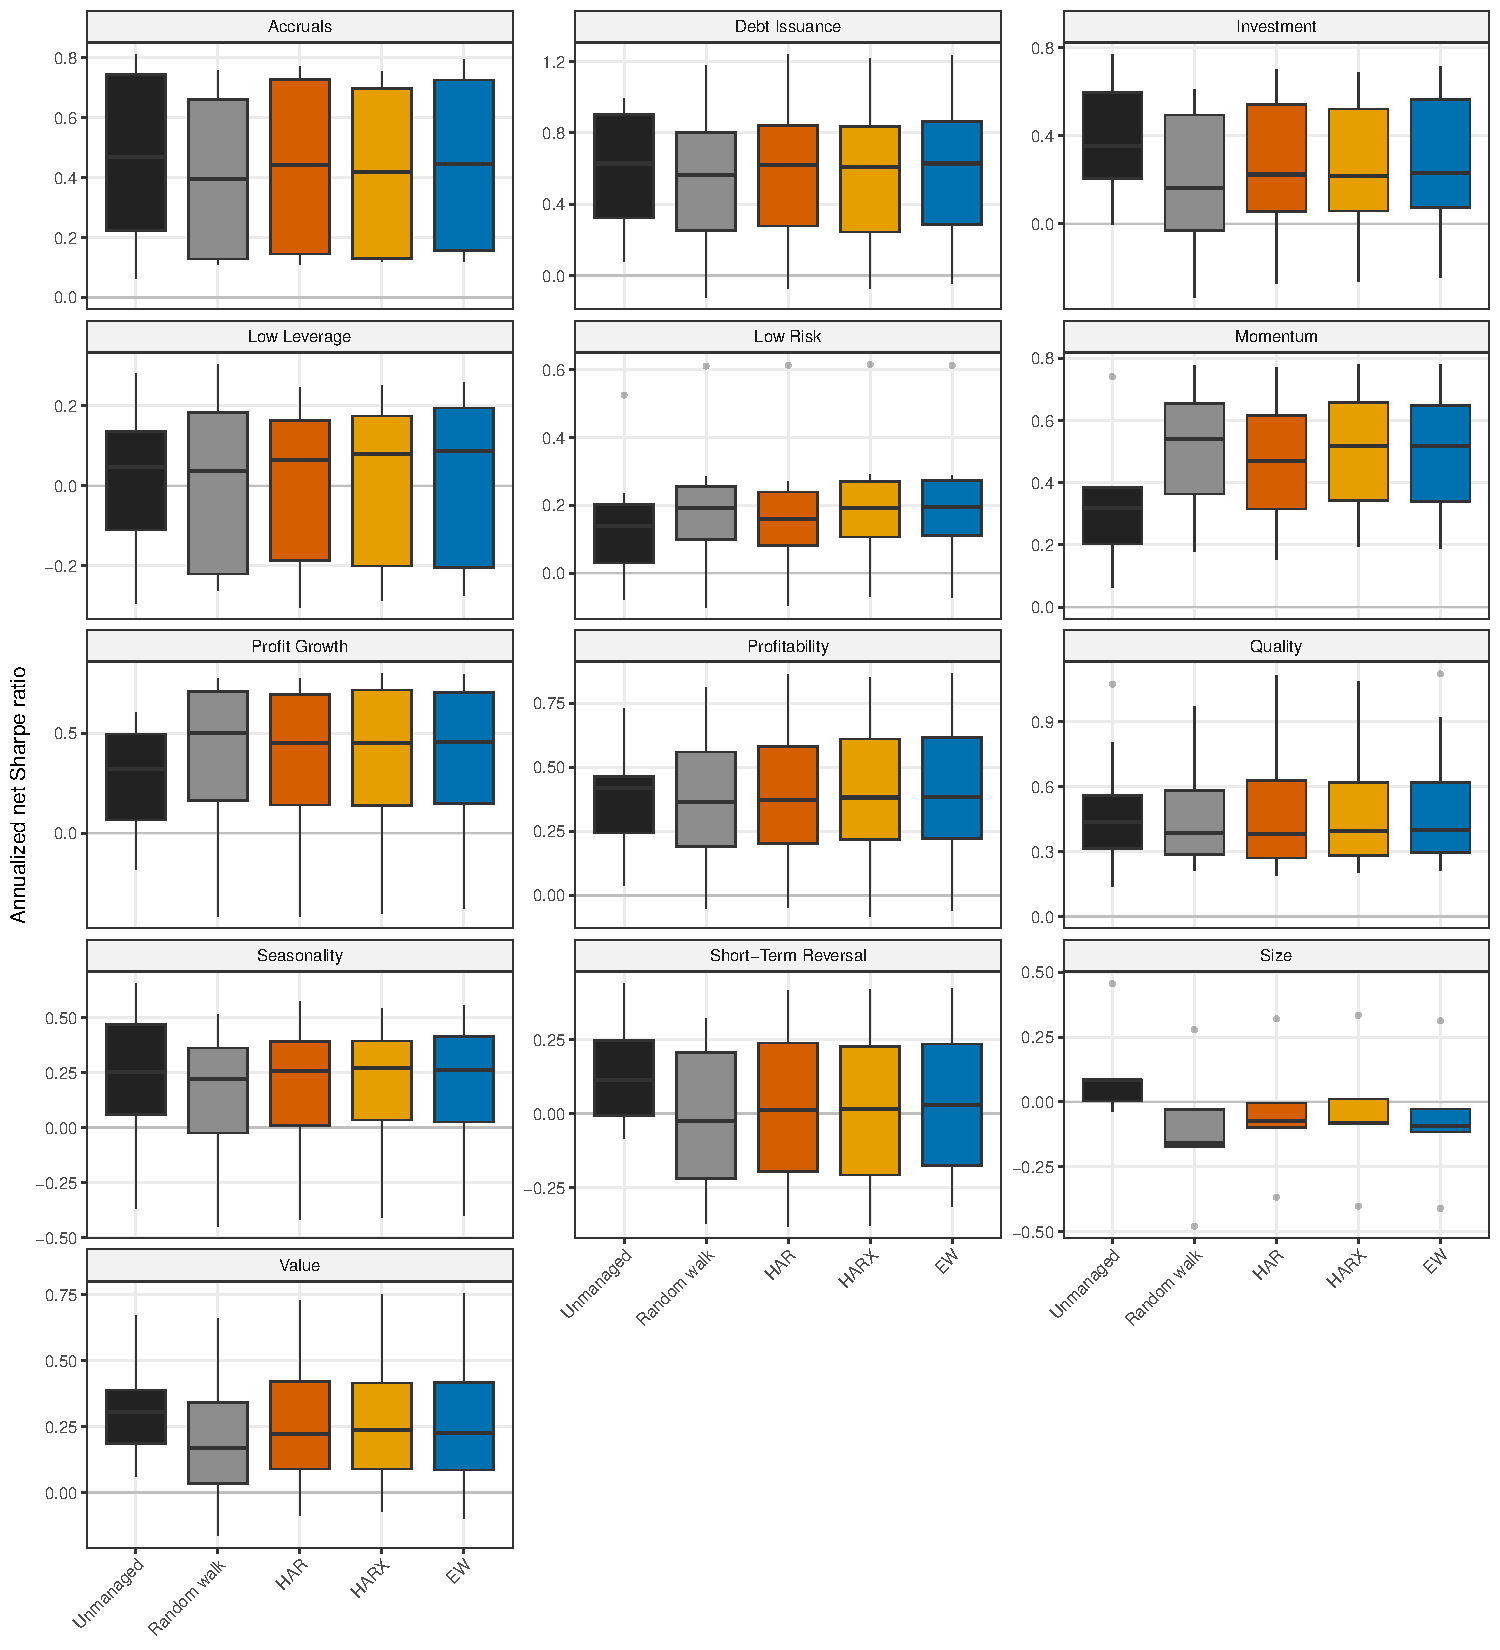
\includegraphics[width=\linewidth,height=0.70\textheight,keepaspectratio]{results_v3/1927/main_appendix/portfolio_cluster_sharpe.pdf}
\end{figure}
\begin{figure}[p]
\ContinuedFloat
\centering
\captionsetup{justification=raggedright,labelsep=none,singlelinecheck=false,labelformat=boldlabel}
\caption[]{\footnotesize \textbf{: Cross-sectional distribution of net Sharpe ratios for volatility-managed factor portfolios by Jensen, Kelly, and Pedersen factor cluster.} Each box summarizes the factor-level Sharpe ratios within the indicated cluster. The center line is the median, the box spans the interquartile range, and the whiskers extend to the most extreme observations within 1.5 interquartile ranges. Managed strategies cap exposure at 1.5 and deduct 10 basis points per unit change in factor exposure. Continued.}
\par\smallskip\textbf{Panel B. Short sample}\par\smallskip
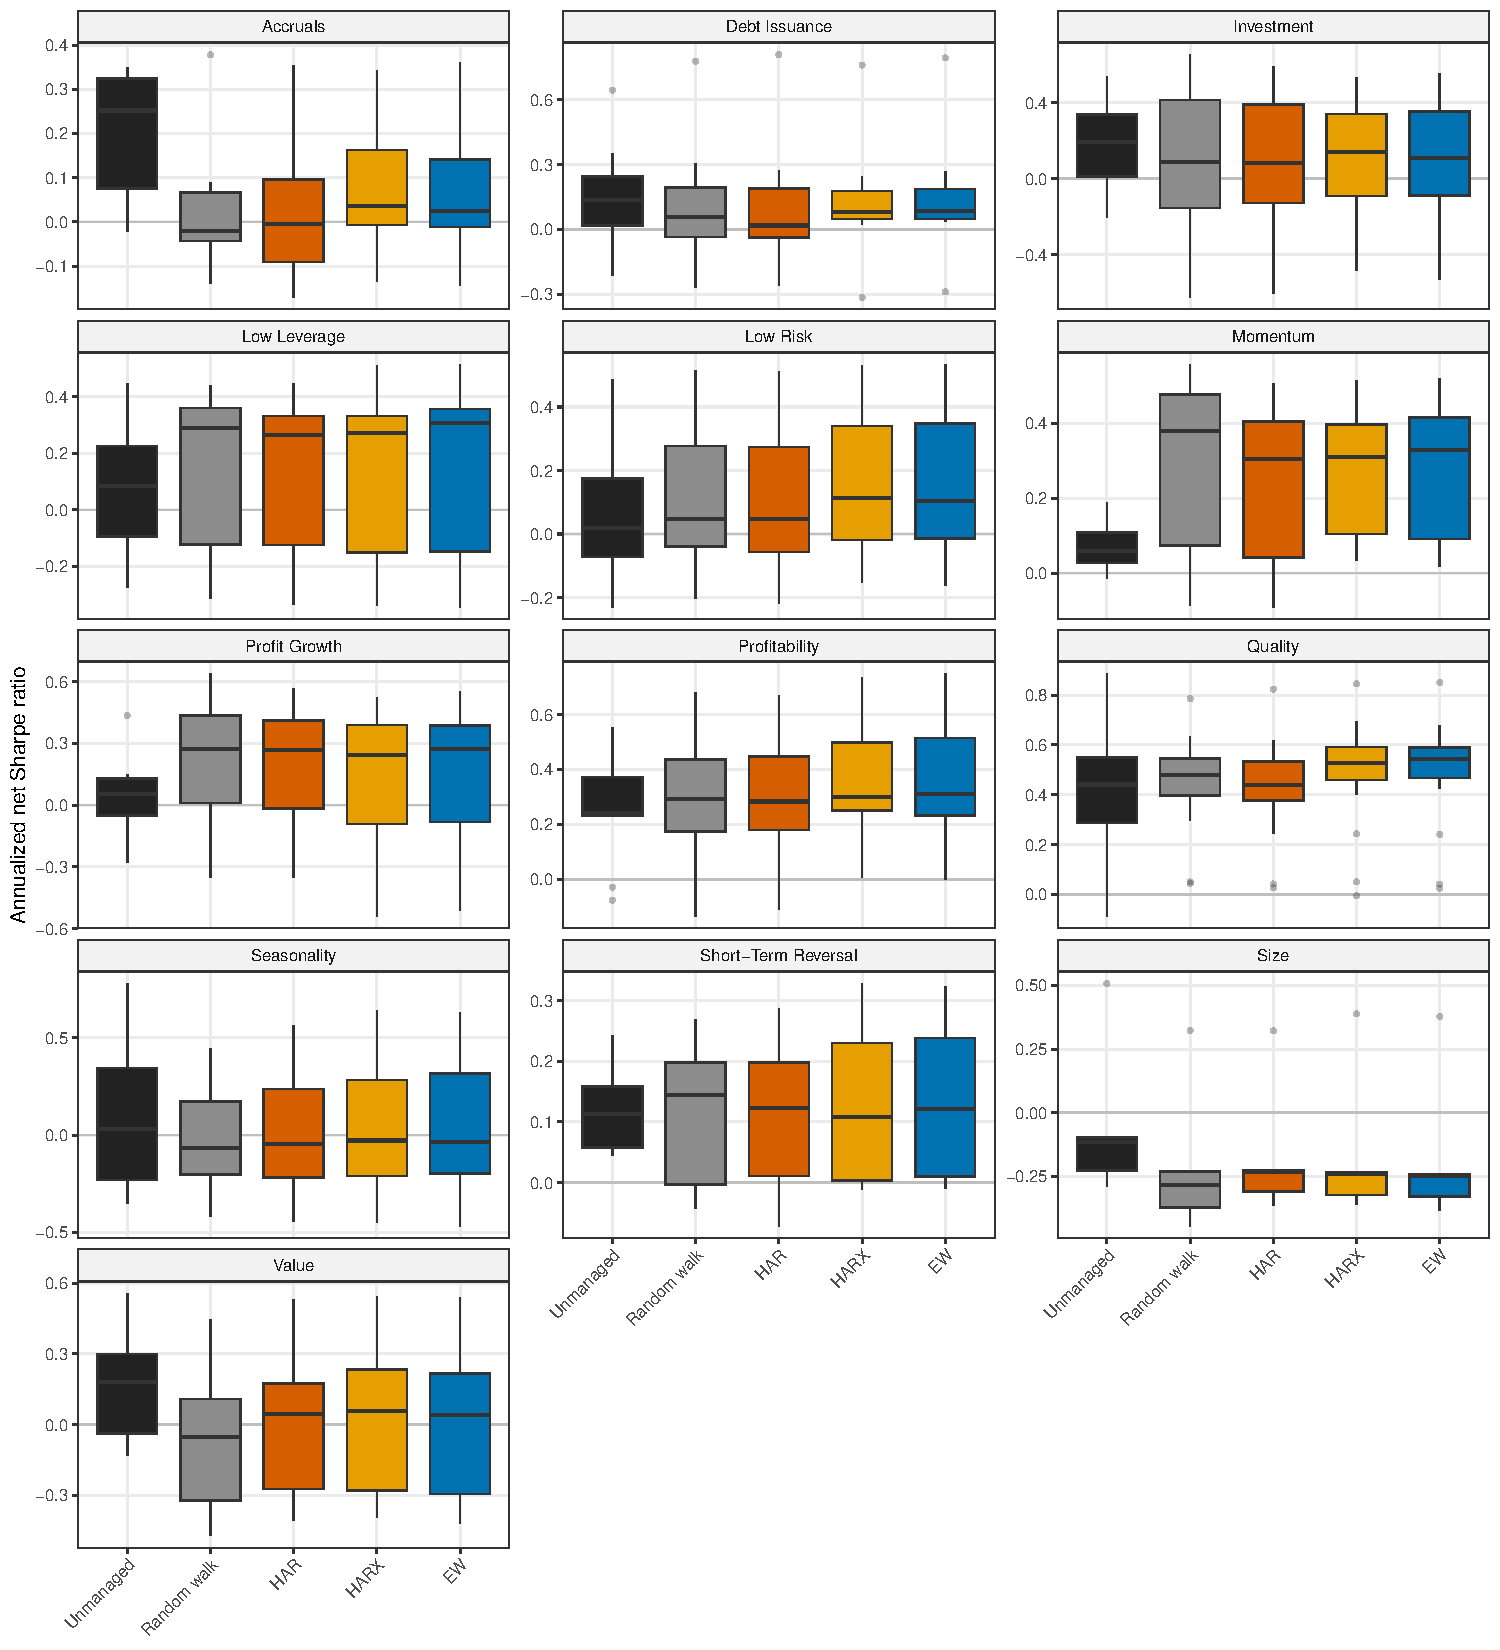
\includegraphics[width=\linewidth,height=0.70\textheight,keepaspectratio]{results_v3/1986/main_appendix/portfolio_cluster_sharpe.pdf}
\end{figure}

\begin{table}[p]
\centering\scriptsize
\captionsetup{justification=raggedright,labelsep=none,singlelinecheck=false,labelformat=boldlabel}
\renewcommand{\arraystretch}{0.91}\setlength{\tabcolsep}{4pt}
\caption[]{\footnotesize \textbf{: Paired Sharpe comparisons for single-factor strategies.} Each row compares the EW forecast ensemble with the stated benchmark, using net returns. Intervals are pointwise 95 percent percentile intervals from 10,000 paired stationary-bootstrap draws with expected block length five months. One-sided p-values use centered bootstrap errors. Holm and Benjamini-Hochberg (BH) adjustments use the same prespecified family across Sharpe, mean and CER, separately within each sample. BH controls the false discovery rate under its dependence assumptions. Inference is conditional on fitted forecasts. Long-sample market strategies span June 1952 to December 2024 and factor aggregates January 1980 to December 2024. Short-sample strategies span July 2011 to December 2024.}
\label{tab:rv-portfolio_inference_single_factor_primary}
\resizebox{\ifdim\width>\linewidth\linewidth\else\width\fi}{!}{%
\begin{tabular}{lrrrrrr}
\multicolumn{7}{@{}l}{\textit{Panel A. Long sample: 50/50 single-factor combination, 153-factor aggregate}} \\
\hline
Benchmark & Exposure & Sharpe difference & 95\% interval & p-value & Holm p-value & BH p-value \\
\hline
Unmanaged & Capped & 0.098 & [0.029, 0.155] & 0.001 & 0.048 & 0.003 \\
RW & Capped & -0.002 & [-0.038, 0.044] & 0.582 & 1.000 & 0.798 \\
HAR & Capped & 0.033 & [0.020, 0.050] & 0.000 & 0.016 & 0.001 \\
HARX & Capped & 0.028 & [0.019, 0.037] & 0.000 & 0.010 & 0.001 \\
Unmanaged & Raw & 0.098 & [0.029, 0.155] & 0.001 & 0.048 & 0.003 \\
RW & Raw & -0.001 & [-0.037, 0.045] & 0.567 & 1.000 & 0.789 \\
HAR & Raw & 0.033 & [0.020, 0.050] & 0.000 & 0.016 & 0.001 \\
HARX & Raw & 0.028 & [0.019, 0.037] & 0.000 & 0.010 & 0.001 \\
\hline
\multicolumn{7}{@{}l}{\textit{Panel B. Long sample: MM management, 153-factor aggregate}} \\
\hline
Benchmark & Exposure & Sharpe difference & 95\% interval & p-value & Holm p-value & BH p-value \\
\hline
Unmanaged & Capped & 0.202 & [0.023, 0.354] & 0.005 & 0.355 & 0.017 \\
RW & Capped & 0.089 & [0.018, 0.159] & 0.009 & 0.587 & 0.028 \\
HAR & Capped & 0.088 & [0.054, 0.122] & 0.000 & 0.010 & 0.001 \\
HARX & Capped & 0.060 & [0.039, 0.082] & 0.000 & 0.010 & 0.001 \\
Unmanaged & Raw & 0.169 & [-0.023, 0.330] & 0.019 & 1.000 & 0.056 \\
RW & Raw & 0.157 & [0.057, 0.257] & 0.001 & 0.086 & 0.005 \\
HAR & Raw & 0.089 & [0.050, 0.129] & 0.000 & 0.010 & 0.001 \\
HARX & Raw & 0.062 & [0.040, 0.085] & 0.000 & 0.010 & 0.001 \\
\hline
\multicolumn{7}{@{}l}{\textit{Panel C. Long sample: 50/50 single-factor combination, Pooled market}} \\
\hline
Benchmark & Exposure & Sharpe difference & 95\% interval & p-value & Holm p-value & BH p-value \\
\hline
Unmanaged & Capped & 0.029 & [-0.031, 0.088] & 0.165 & 1.000 & 0.343 \\
RW & Capped & 0.009 & [-0.065, 0.088] & 0.409 & 1.000 & 0.650 \\
HAR & Capped & 0.002 & [-0.013, 0.017] & 0.401 & 1.000 & 0.650 \\
HARX & Capped & 0.001 & [-0.010, 0.011] & 0.438 & 1.000 & 0.667 \\
Unmanaged & Raw & 0.029 & [-0.031, 0.088] & 0.165 & 1.000 & 0.343 \\
RW & Raw & 0.006 & [-0.070, 0.085] & 0.449 & 1.000 & 0.673 \\
HAR & Raw & 0.002 & [-0.013, 0.017] & 0.401 & 1.000 & 0.650 \\
HARX & Raw & 0.001 & [-0.010, 0.011] & 0.438 & 1.000 & 0.667 \\
\hline
\multicolumn{7}{@{}l}{\textit{Panel D. Long sample: MM management, Pooled market}} \\
\hline
Benchmark & Exposure & Sharpe difference & 95\% interval & p-value & Holm p-value & BH p-value \\
\hline
Unmanaged & Capped & 0.021 & [-0.104, 0.147] & 0.362 & 1.000 & 0.632 \\
RW & Capped & 0.006 & [-0.044, 0.056] & 0.413 & 1.000 & 0.650 \\
HAR & Capped & -0.003 & [-0.032, 0.027] & 0.566 & 1.000 & 0.789 \\
HARX & Capped & -0.008 & [-0.028, 0.013] & 0.777 & 1.000 & 0.990 \\
Unmanaged & Raw & 0.024 & [-0.107, 0.155] & 0.347 & 1.000 & 0.616 \\
RW & Raw & 0.060 & [-0.046, 0.168] & 0.135 & 1.000 & 0.302 \\
HAR & Raw & 0.000 & [-0.033, 0.034] & 0.489 & 1.000 & 0.712 \\
HARX & Raw & -0.001 & [-0.023, 0.021] & 0.518 & 1.000 & 0.742 \\
\hline
\end{tabular}}
\end{table}
\begin{table}[p]
\ContinuedFloat
\centering\scriptsize
\captionsetup{justification=raggedright,labelsep=none,singlelinecheck=false,labelformat=boldlabel}
\renewcommand{\arraystretch}{0.91}\setlength{\tabcolsep}{4pt}
\caption[]{\footnotesize \textbf{: Paired Sharpe comparisons for single-factor strategies. Continued.} Short-sample results. Definitions and conventions follow the preceding panels.}
\resizebox{\ifdim\width>\linewidth\linewidth\else\width\fi}{!}{%
\begin{tabular}{lrrrrrr}
\multicolumn{7}{@{}l}{\textit{Panel E. Short sample: 50/50 single-factor combination, 153-factor aggregate}} \\
\hline
Benchmark & Exposure & Sharpe difference & 95\% interval & p-value & Holm p-value & BH p-value \\
\hline
Unmanaged & Capped & 0.018 & [-0.104, 0.152] & 0.379 & 1.000 & 0.568 \\
RW & Capped & 0.035 & [-0.034, 0.098] & 0.134 & 1.000 & 0.380 \\
HAR & Capped & 0.021 & [-0.023, 0.061] & 0.148 & 1.000 & 0.384 \\
HARX & Capped & 0.031 & [0.006, 0.058] & 0.012 & 1.000 & 0.177 \\
Unmanaged & Raw & 0.018 & [-0.104, 0.152] & 0.379 & 1.000 & 0.568 \\
RW & Raw & 0.035 & [-0.034, 0.098] & 0.134 & 1.000 & 0.380 \\
HAR & Raw & 0.021 & [-0.023, 0.061] & 0.148 & 1.000 & 0.384 \\
HARX & Raw & 0.031 & [0.006, 0.058] & 0.012 & 1.000 & 0.177 \\
\hline
\multicolumn{7}{@{}l}{\textit{Panel F. Short sample: 50/50 single-factor combination, Pooled market}} \\
\hline
Benchmark & Exposure & Sharpe difference & 95\% interval & p-value & Holm p-value & BH p-value \\
\hline
Unmanaged & Capped & 0.016 & [-0.168, 0.201] & 0.411 & 1.000 & 0.589 \\
RW & Capped & 0.083 & [-0.100, 0.269] & 0.181 & 1.000 & 0.425 \\
HAR & Capped & 0.018 & [-0.086, 0.132] & 0.358 & 1.000 & 0.554 \\
HARX & Capped & 0.000 & [-0.040, 0.040] & 0.486 & 1.000 & 0.639 \\
Unmanaged & Raw & 0.016 & [-0.168, 0.201] & 0.411 & 1.000 & 0.589 \\
RW & Raw & 0.083 & [-0.100, 0.269] & 0.181 & 1.000 & 0.425 \\
HAR & Raw & 0.018 & [-0.086, 0.132] & 0.358 & 1.000 & 0.554 \\
HARX & Raw & 0.000 & [-0.040, 0.040] & 0.486 & 1.000 & 0.639 \\
\hline
\multicolumn{7}{@{}l}{\textit{Panel G. Short sample: MM management, 153-factor aggregate}} \\
\hline
Benchmark & Exposure & Sharpe difference & 95\% interval & p-value & Holm p-value & BH p-value \\
\hline
Unmanaged & Capped & 0.043 & [-0.188, 0.312] & 0.356 & 1.000 & 0.554 \\
RW & Capped & 0.152 & [-0.029, 0.341] & 0.054 & 1.000 & 0.236 \\
HAR & Capped & 0.058 & [-0.026, 0.136] & 0.072 & 1.000 & 0.276 \\
HARX & Capped & 0.021 & [-0.014, 0.057] & 0.116 & 1.000 & 0.380 \\
Unmanaged & Raw & -0.012 & [-0.285, 0.299] & 0.521 & 1.000 & 0.652 \\
RW & Raw & 0.138 & [-0.062, 0.349] & 0.090 & 1.000 & 0.331 \\
HAR & Raw & 0.039 & [-0.050, 0.125] & 0.182 & 1.000 & 0.425 \\
HARX & Raw & 0.065 & [0.014, 0.115] & 0.004 & 0.432 & 0.177 \\
\hline
\multicolumn{7}{@{}l}{\textit{Panel H. Short sample: MM management, Pooled market}} \\
\hline
Benchmark & Exposure & Sharpe difference & 95\% interval & p-value & Holm p-value & BH p-value \\
\hline
Unmanaged & Capped & -0.010 & [-0.265, 0.243] & 0.503 & 1.000 & 0.652 \\
RW & Capped & 0.068 & [-0.162, 0.292] & 0.287 & 1.000 & 0.530 \\
HAR & Capped & -0.068 & [-0.162, 0.025] & 0.924 & 1.000 & 0.924 \\
HARX & Capped & 0.028 & [-0.033, 0.077] & 0.134 & 1.000 & 0.380 \\
Unmanaged & Raw & -0.039 & [-0.364, 0.287] & 0.570 & 1.000 & 0.684 \\
RW & Raw & 0.233 & [-0.120, 0.522] & 0.054 & 1.000 & 0.236 \\
HAR & Raw & 0.040 & [-0.140, 0.208] & 0.300 & 1.000 & 0.544 \\
HARX & Raw & 0.010 & [-0.057, 0.077] & 0.393 & 1.000 & 0.581 \\
\hline
\end{tabular}}
\end{table}

\begin{table}[p]
\centering\scriptsize
\captionsetup{justification=raggedright,labelsep=none,singlelinecheck=false,labelformat=boldlabel}
\renewcommand{\arraystretch}{0.91}\setlength{\tabcolsep}{4pt}
\caption[]{\footnotesize \textbf{: Paired Sharpe comparisons for multifactor strategies.} Each row compares the EW forecast ensemble with the stated benchmark, using net returns. Intervals are pointwise 95 percent percentile intervals from 10,000 paired stationary-bootstrap draws with expected block length five months. One-sided p-values use centered bootstrap errors. Holm and Benjamini-Hochberg (BH) adjustments use the same prespecified family across Sharpe, mean and CER, separately within each sample. BH controls the false discovery rate under its dependence assumptions. Inference is conditional on fitted forecasts. Long-sample evaluation spans January 1980 to December 2024. Short-sample evaluation spans July 2011 to December 2024.}
\label{tab:rv-portfolio_inference_multifactor_primary}
\resizebox{\ifdim\width>\linewidth\linewidth\else\width\fi}{!}{%
\begin{tabular}{lrrrrrr}
\multicolumn{7}{@{}l}{\textit{Panel A. Long sample: EW allocation, CMV, pooled market}} \\
\hline
Benchmark & Exposure & Sharpe difference & 95\% interval & p-value & Holm p-value & BH p-value \\
\hline
UMV & Raw & 0.046 & [0.010, 0.071] & 0.000 & 0.015 & 0.001 \\
Lagged market & Raw & -0.017 & [-0.039, 0.018] & 0.937 & 1.000 & 0.999 \\
HAR & Raw & 0.008 & [0.001, 0.014] & 0.007 & 0.461 & 0.025 \\
HARX & Raw & 0.008 & [0.000, 0.013] & 0.005 & 0.356 & 0.023 \\
UMV & Capped & 0.046 & [0.010, 0.071] & 0.000 & 0.015 & 0.001 \\
Lagged market & Capped & -0.017 & [-0.038, 0.018] & 0.939 & 1.000 & 0.999 \\
HAR & Capped & 0.008 & [0.001, 0.014] & 0.007 & 0.461 & 0.025 \\
HARX & Capped & 0.008 & [0.000, 0.013] & 0.005 & 0.356 & 0.023 \\
\hline
\multicolumn{7}{@{}l}{\textit{Panel B. Long sample: EW allocation, FCMV}} \\
\hline
Benchmark & Exposure & Sharpe difference & 95\% interval & p-value & Holm p-value & BH p-value \\
\hline
UMV & Raw & 0.060 & [0.014, 0.093] & 0.000 & 0.029 & 0.002 \\
HAR & Raw & 0.019 & [0.012, 0.028] & 0.000 & 0.008 & 0.001 \\
HARX & Raw & 0.014 & [0.009, 0.019] & 0.000 & 0.008 & 0.001 \\
UMV & Capped & 0.060 & [0.014, 0.093] & 0.000 & 0.029 & 0.002 \\
HAR & Capped & 0.019 & [0.012, 0.028] & 0.000 & 0.008 & 0.001 \\
HARX & Capped & 0.014 & [0.009, 0.019] & 0.000 & 0.008 & 0.001 \\
\hline
\multicolumn{7}{@{}l}{\textit{Panel C. Long sample: HEW allocation, CMV, pooled market}} \\
\hline
Benchmark & Exposure & Sharpe difference & 95\% interval & p-value & Holm p-value & BH p-value \\
\hline
UMV & Raw & 0.056 & [-0.031, 0.100] & 0.007 & 0.461 & 0.025 \\
Lagged market & Raw & -0.019 & [-0.068, 0.066] & 0.775 & 1.000 & 0.999 \\
HAR & Raw & 0.016 & [0.006, 0.026] & 0.001 & 0.077 & 0.006 \\
HARX & Raw & 0.020 & [-0.002, 0.033] & 0.002 & 0.122 & 0.008 \\
UMV & Capped & 0.056 & [-0.031, 0.100] & 0.007 & 0.461 & 0.025 \\
Lagged market & Capped & -0.021 & [-0.068, 0.061] & 0.805 & 1.000 & 0.999 \\
HAR & Capped & 0.016 & [0.006, 0.026] & 0.001 & 0.077 & 0.006 \\
HARX & Capped & 0.020 & [-0.002, 0.033] & 0.002 & 0.122 & 0.008 \\
\hline
\multicolumn{7}{@{}l}{\textit{Panel D. Long sample: HEW allocation, FCMV}} \\
\hline
Benchmark & Exposure & Sharpe difference & 95\% interval & p-value & Holm p-value & BH p-value \\
\hline
UMV & Raw & 0.131 & [0.024, 0.183] & 0.000 & 0.008 & 0.001 \\
HAR & Raw & 0.029 & [0.018, 0.042] & 0.000 & 0.008 & 0.001 \\
HARX & Raw & 0.027 & [0.012, 0.036] & 0.000 & 0.008 & 0.001 \\
UMV & Capped & 0.131 & [0.024, 0.183] & 0.000 & 0.008 & 0.001 \\
HAR & Capped & 0.029 & [0.018, 0.042] & 0.000 & 0.008 & 0.001 \\
HARX & Capped & 0.027 & [0.012, 0.036] & 0.000 & 0.008 & 0.001 \\
\hline
\end{tabular}}
\end{table}
\begin{table}[p]
\ContinuedFloat
\centering\scriptsize
\captionsetup{justification=raggedright,labelsep=none,singlelinecheck=false,labelformat=boldlabel}
\renewcommand{\arraystretch}{0.91}\setlength{\tabcolsep}{4pt}
\caption[]{\footnotesize \textbf{: Paired Sharpe comparisons for multifactor strategies. Continued.} Short-sample results. Definitions and conventions follow the preceding panels.}
\resizebox{\ifdim\width>\linewidth\linewidth\else\width\fi}{!}{%
\begin{tabular}{lrrrrrr}
\multicolumn{7}{@{}l}{\textit{Panel E. Short sample: EW allocation, CMV, pooled market}} \\
\hline
Benchmark & Exposure & Sharpe difference & 95\% interval & p-value & Holm p-value & BH p-value \\
\hline
UMV & Raw & 0.000 & [-0.070, 0.071] & 0.479 & 1.000 & 0.529 \\
Lagged market & Raw & 0.021 & [-0.038, 0.075] & 0.215 & 1.000 & 0.365 \\
HAR & Raw & 0.020 & [-0.010, 0.048] & 0.078 & 1.000 & 0.365 \\
HARX & Raw & 0.012 & [-0.005, 0.030] & 0.101 & 1.000 & 0.365 \\
UMV & Capped & 0.000 & [-0.070, 0.071] & 0.479 & 1.000 & 0.529 \\
Lagged market & Capped & 0.021 & [-0.030, 0.067] & 0.183 & 1.000 & 0.365 \\
HAR & Capped & 0.020 & [-0.010, 0.048] & 0.078 & 1.000 & 0.365 \\
HARX & Capped & 0.011 & [-0.006, 0.030] & 0.104 & 1.000 & 0.365 \\
\hline
\multicolumn{7}{@{}l}{\textit{Panel F. Short sample: EW allocation, FCMV}} \\
\hline
Benchmark & Exposure & Sharpe difference & 95\% interval & p-value & Holm p-value & BH p-value \\
\hline
UMV & Raw & 0.026 & [-0.039, 0.099] & 0.221 & 1.000 & 0.365 \\
HAR & Raw & 0.016 & [-0.009, 0.038] & 0.072 & 1.000 & 0.365 \\
HARX & Raw & 0.013 & [0.001, 0.027] & 0.027 & 1.000 & 0.365 \\
UMV & Capped & 0.026 & [-0.039, 0.099] & 0.221 & 1.000 & 0.365 \\
HAR & Capped & 0.016 & [-0.009, 0.038] & 0.072 & 1.000 & 0.365 \\
HARX & Capped & 0.013 & [0.001, 0.027] & 0.027 & 1.000 & 0.365 \\
\hline
\multicolumn{7}{@{}l}{\textit{Panel G. Short sample: HEW allocation, CMV, pooled market}} \\
\hline
Benchmark & Exposure & Sharpe difference & 95\% interval & p-value & Holm p-value & BH p-value \\
\hline
UMV & Raw & -0.022 & [-0.105, 0.053] & 0.670 & 1.000 & 0.670 \\
Lagged market & Raw & 0.067 & [0.002, 0.134] & 0.027 & 1.000 & 0.365 \\
HAR & Raw & 0.038 & [-0.001, 0.077] & 0.030 & 1.000 & 0.365 \\
HARX & Raw & 0.014 & [-0.004, 0.035] & 0.091 & 1.000 & 0.365 \\
UMV & Capped & -0.022 & [-0.105, 0.053] & 0.670 & 1.000 & 0.670 \\
Lagged market & Capped & 0.050 & [-0.004, 0.105] & 0.040 & 1.000 & 0.365 \\
HAR & Capped & 0.038 & [-0.001, 0.077] & 0.030 & 1.000 & 0.365 \\
HARX & Capped & 0.013 & [-0.004, 0.033] & 0.091 & 1.000 & 0.365 \\
\hline
\multicolumn{7}{@{}l}{\textit{Panel H. Short sample: HEW allocation, FCMV}} \\
\hline
Benchmark & Exposure & Sharpe difference & 95\% interval & p-value & Holm p-value & BH p-value \\
\hline
UMV & Raw & 0.041 & [-0.057, 0.127] & 0.161 & 1.000 & 0.365 \\
HAR & Raw & 0.030 & [-0.007, 0.070] & 0.070 & 1.000 & 0.365 \\
HARX & Raw & 0.018 & [-0.002, 0.040] & 0.049 & 1.000 & 0.365 \\
UMV & Capped & 0.041 & [-0.057, 0.127] & 0.161 & 1.000 & 0.365 \\
HAR & Capped & 0.030 & [-0.007, 0.070] & 0.070 & 1.000 & 0.365 \\
HARX & Capped & 0.018 & [-0.002, 0.040] & 0.049 & 1.000 & 0.365 \\
\hline
\end{tabular}}
\end{table}



\clearpage

\section{Internet Appendix}

\setcounter{table}{0}
\renewcommand{\thetable}{IA.\arabic{table}}
\renewcommand{\theHtable}{IA.\arabic{table}}
\setcounter{figure}{0}
\renewcommand{\thefigure}{IA.\arabic{figure}}
\renewcommand{\theHfigure}{IA.\arabic{figure}}
\setcounter{equation}{0}
\renewcommand{\theequation}{IA.\arabic{equation}}
\renewcommand{\theHequation}{IA.\arabic{equation}}


\subsection{Forecasting Design Details}\label{app:algorithmic}

Following equation~\eqref{eq:model}, $\mathbf{x}_{i,t}$ denotes the
series-specific predictor block, $\mathbf{c}_t$ denotes the common
calendar-time block, and $\ell_{i,t}$ denotes the expanding series-level RV
term. We use $\mathbf{z}^{P}_{i,t}=(\mathbf{x}_{i,t}^{\top},
\mathbf{c}_{t}^{\top},\ell_{i,t})^{\top}$ for the pooled panel and
$\mathbf{z}^{M}_{t}=(\mathbf{x}_{M,t}^{\top},\mathbf{c}_{t}^{\top})^{\top}$
for the standalone market model. Pooled-model parameters are common across the
154 return series. 

The main results use the predictor sample beginning in 1927, grid search, and rescaling of predictors using the min-max transformation. The short sample beginning in 1986 applies the same estimation and reporting procedures with additional covariates, including option-implied volatility. It provides a comparison with a richer information set over a shorter evaluation period.

Both samples retain the same model classes, forecast-ensemble membership, loss functions, and portfolio definitions.

\subsubsection{Preprocessing}

The raw common predictors $\mathbf{c}_t$ have the same value for every return
series observed in month $t$. They are joined to each series by month and, like
the series-specific predictors, are then winsorized and rescaled using that
series' available expanding history with min-max transformation. For a general variable $x_{i,t}$, we thus apply:

\[
x^{*}_{i,j,t}
=
2\left(
\frac{x_{i,j,t}-\min_{s<t}x_{i,j,s}}
{\max_{s<t}x_{i,j,s}-\min_{s<t}x_{i,j,s}}
\right)-1,
\]

For $\mathbf{c}_t$, we apply the same procedure involving each series point-in-time past history, with special attention to the release shedule of macroeconomic indicators.

We require a minimum of 36 observations before transformed rows are retained. Except for jump and negative-return variations, variance-family predictors
are logged before these operations.

The code constructs $\ell_{i,t}$ after that
log transformation as the expanding mean of the lagged monthly-RV predictor
within series, but excludes it from subsequent winsorization and rescaling. This
preserves the cross-sectional level information that preprocessing the other
columns within series removes. Calendar variables are also not transformed.

For readability, the model equations below retain the economic labels of the
predictors, although each regressor entering estimation is its point-in-time
transformed counterpart described above.


\subsubsection{Hyperparameter search}

Hyperparameters are selected on a validation block of the 90 months immediately preceding the forecast date, chosen once a year in June, and the selected configuration is then refitted on all data up to month $t$ before month $t+1$ is forecast. The heterogeneous autoregressive specifications have no hyperparameters and are refitted on the same expanding window without a validation block. Their training requirement is thus set to 210 months, which equals the 120 initial training months and 90 validation months the tuned models consume, so every specification produces its first forecast in the same month and the comparison is never contaminated by a difference in the evaluation window.

Hyperparameters are selected via grid search. It evaluates every combination in Table~\ref{tab:hyper} and selects the one that minimizes root mean squared error on the validation block. The complete grid, fixed settings and number of combinations per refit are reported in Table~\ref{tab:hyper}.

The models used are described as follows.

\subsubsection{Linear models}

The HAR benchmark of \citet{corsi2009} uses the daily,
weekly, and monthly logged realized-variance terms. The pooled version also
includes the expanding series-level term:
\begin{equation}
\begin{aligned}
g_{\mathrm{HAR},u}(\mathbf{z}^{u}_{i,t})
={}& \beta_0 + \beta_d \log RV^{(d)}_{i,t}
 + \beta_w \log RV^{(w)}_{i,t}\\
&+ \beta_m \log RV^{(m)}_{i,t}
 + \mathbf{1}\{u=P\}\gamma\ell_{i,t},
\qquad u\in\{P,M\}.
\end{aligned}
\end{equation}
The augmented HARX specification applies ordinary least squares to the full predictor vector:
\begin{equation}
g_{\mathrm{HARX},u}(\mathbf{z}^{u}_{i,t})
=
\beta_{0,u}
+
(\mathbf{z}^{u}_{i,t})^{\top}\boldsymbol{\theta}_{u},
\qquad u\in\{P,M\},
\end{equation}
where $\boldsymbol{\theta}_{u}$ is the vector of regression coefficients associated with the predictors in $\mathbf{z}^{u}_{i,t}$.

 The elastic net minimizes squared error plus a mixture of the two penalties:
\begin{equation}
	\begin{aligned}
		g_{\mathrm{ENET},u}(\mathbf{z}^{u}_{i,t})
		&=
		\widehat{\beta}_{0,u}
		+
		(\mathbf{z}^{u}_{i,t})^{\top}
		\widehat{\boldsymbol{\theta}}_{u},\\
		(\widehat{\beta}_{0,u},\widehat{\boldsymbol{\theta}}_{u})
		&=
		\arg\min_{\beta_0,\boldsymbol{\theta}}
		\Bigg\{
		\frac{1}{2N_u}
		\sum_{(i,t)\in\mathcal{T}_u}
		\left[
		y_{i,t+1}-\beta_0
		-(\mathbf{z}^{u}_{i,t})^{\top}\boldsymbol{\theta}
		\right]^2\\
		&\hspace{2.5cm}
		+
		\lambda
		\left[
		\alpha\lVert\boldsymbol{\theta}\rVert_1
		+
		\frac{1-\alpha}{2}
		\lVert\boldsymbol{\theta}\rVert_2^2
		\right]
		\Bigg\},
		\qquad u\in\{P,M\}.
	\end{aligned}
\end{equation}
with $\alpha$ and $\lambda$ tuned. In particular, $\lambda$ chosen on the fitted regularization path with a minimum ratio of $10^{-4}$.

\subsubsection{Tree ensembles}

A regression tree partitions the predictor space into terminal regions $C_l$ and assigns each observation the mean outcome in its region, \begin{equation}
g_{\mathrm{RF},u}(\mathbf{z}^{u}_{i,t}) = \sum_{l=1}^{L} \theta_l
 \mathbf{1}\{\mathbf{z}^{u}_{i,t} \in C_l\}.
\end{equation}
The random forest averages trees grown on bootstrap resamples, with a random
fraction of predictors considered at each split, which decorrelates the trees
and reduces variance. In pooled random forests, $\ell_{i,t}$ is always included
among the candidate split variables in addition to the randomly sampled subset,
because it is the only design-matrix column carrying persistent series-level
information. Gradient boosting instead constructs an additive sequence,
\begin{equation}
g_{\mathrm{XGB},u}(\mathbf{z}^{u}_{i,t}) = \sum_{f=1}^{F} T_f(\mathbf{z}^{u}_{i,t}),
\end{equation}
in which each new tree is fitted to the remaining loss from the preceding ensemble. Depth governs the order of interaction, the learning rate scales the contribution of each tree, and the regularized objective penalizes leaf
complexity and leaf weights \citep{chenguestrin2016}. The number of rounds is set by early stopping after 30 rounds without validation improvement rather than tuned, so the round count in Table~\ref{tab:hyper} is a ceiling.

\subsubsection{Neural networks}

The networks are feedforward with ReLU activations,
\begin{equation}
g_{\mathrm{NN},u}(\mathbf{z}^{u}_{i,t}) = \mathbf{W}_{K}\operatorname{ReLU}
 \bigl(\cdots \operatorname{ReLU}(\mathbf{W}_{1}\mathbf{z}^{u}_{i,t} +
 \mathbf{b}_{1}) \cdots \bigr) + \mathbf{b}_{K},
\end{equation}
with batch normalization at each hidden layer. NN1 has one hidden layer of 32 units, NN2 has layers of 32 and 16 units, and NN3 has layers of 32, 16 and 8 units. Training uses Adam and minimizes squared error plus an $L_1$ penalty on
the weights,
\begin{equation}
\mathcal{L}_{\mathrm{NN}} = \sum_{i,t}
 \bigl[y_{i,t+1} - g_{\mathrm{NN},u}(\mathbf{z}^{u}_{i,t})\bigr]^{2}
 + \lambda^{\omega} \sum_k \lVert \mathbf{W}_k \rVert_1,
\end{equation}
stopping after 10 epochs without validation improvement. After hyperparameters are selected, each architecture is refitted from ten independent random initializations and the predictions are averaged, following \citet{gukellyxiu2020}. Tuning itself uses a single fitted network, so the averaging reduces sensitivity to one initialization without enlarging the search budget.

\subsubsection{Ensemble}

The equal-weighted ensemble averages the seven constituent model forecasts in log realized-variance space:
\begin{equation}
g_{\mathrm{EW},u}(\mathbf{z}^{u}_{i,t})
=
\frac{1}{|\mathcal{M}|}
\sum_{m\in\mathcal{M}}
g_{m,u}(\mathbf{z}^{u}_{i,t})
\end{equation}

where $|\mathcal{M}|=\{\mathrm{HARX},\mathrm{ENET},\mathrm{RF},\mathrm{XGB},
\mathrm{NN1},\mathrm{NN2},\mathrm{NN3}\}$. 
The corresponding forecast in realized-variance units is
\[
\widehat{RV}^{\mathrm{EW}}_{i,t+1}
=
\exp\!\left[
g_{\mathrm{EW},u}(\mathbf{z}^{u}_{i,t})
\right].
\]

\subsection{Portfolio Application Details}
\label{app:portfolio-design}

The portfolio exercises are adaptations rather than exact replications of the original studies. In this section, we outline the main differences in applications and also detail the computation of performance statistics and spanning regressions.

\subsubsection{Single-factor normalization and diagnostics}

Equation~\eqref{eq:managed} uses at least 60 prior paired observations and an expanding history. The time-varying normalizer gives the managed and unmanaged series the same volatility over the information set available before month $t$, but it does not impose equal realized volatility over the subsequent evaluation sample. \citet{moreiramuir2017} instead choose a constant $c_i^{*}$ that equates the two volatilities over their full sample. They note that this scale does not affect the managed portfolio's Sharpe ratio. The full-sample value is nevertheless unavailable when the position is formed and can affect exposures, binding caps, turnover, and costs. We therefore use the real-time design of \citet{cederburg2020}.

The unconstrained Moreira-Muir exposure is $w^{\mathrm{MM}}_{i,t}=c_{i,t}/\widehat{\sigma}^{\,2}_{i,t\mid t-1}$. Their main return analysis is unconstrained, while their leverage robustness exercises cap this exposure at 1.5. They interpret 1.5 as a standard margin constraint allowing 50\% leverage. We report the raw exposure and the corresponding capped specification,
\begin{equation}
w^{\mathrm{MM,cap}}_{i,t}
=\min\left\{1.5,w^{\mathrm{MM}}_{i,t}\right\}.
\end{equation}

Spanning regressions take the form
\begin{equation}
\widetilde{f}_{i,t} = \alpha_i + \beta_i f_{i,t} + u_{i,t}.
\label{eq:spanning}
\end{equation}
We use Newey--West inference for the intercept and report the annualized appraisal ratio $\widehat{AR}_i=\sqrt{12}\widehat{\alpha}_i/\widehat{\sigma}_{u_i}$. These quantities are ex-post opportunity-set diagnostics. A nonzero alpha indicates that adding the managed return changes the ex-post mean-variance frontier. As emphasized by \citet{cederburg2020}, the corresponding tangency portfolio is an ex-post optimal combination of the unmanaged and managed returns. The regression does not establish that the managed return alone dominates, and the optimal combination is not known to a real-time investor.

\subsubsection{\citet{cederburg2020} allocation and exposure constraint}

The signed two-sleeve MVO reported in the Internet Appendix estimates $a_{i,t}$ and $b_{i,t}$ from the expanding training matrix and forms
\begin{equation}
f^{\mathrm{MVO}}_{i,t}
=\left(a_{i,t}+b_{i,t}
\frac{c_{i,t}}{\widehat{\sigma}^{\,2}_{i,t\mid t-1}}\right)f_{i,t}.
\label{eq:cederburg-mvo}
\end{equation}
The current normalizer $c_{i,t}$ is applied to every managed-sleeve observation in that training matrix. We consider a paired benchmark that estimates only the coefficient on the unmanaged factor over the same history and sets $b_{i,t}=0$. Neither single-factor Neither single-factor MVO imposes that the two sleeve coefficients sum to one. The optimization therefore selects the scale of a self-financing factor overlay rather than a fully invested allocation across the two sleeves. Total returns add the risk-free return on one unit of collateral to the resulting factor payoff

This leverage constraint matches the object defined by \citet{cederburg2020}. In their notation, $x_{\sigma,i,t}$ and $x_{i,t}$ are the MVO coefficients on the managed and unmanaged sleeves. The actual position in the underlying factor is
\begin{equation}
y_{i,t}
=x_{i,t}
+x_{\sigma,i,t}
\frac{c_{i,t}}{\widehat{\sigma}^{\,2}_{i,t\mid t-1}}.
\end{equation}
\citet{cederburg2020} impose $|y_{i,t}|\leq5$. Our notation sets $a_{i,t}=x_{i,t}$ and $b_{i,t}=x_{\sigma,i,t}$, so $w^{\mathrm{Ced}}_{i,t}=y_{i,t}$. The saved implementation therefore applies the same base-case constraint,
\begin{equation}
w^{\mathrm{Ced,cap}}_{i,t}
=\max\left\{-5,\min\left(5,w^{\mathrm{Ced}}_{i,t}\right)\right\}.
\end{equation}

Our fixed 50/50 extension sets $a_{i,t}=b_{i,t}=1/2$ and applies the same bound to its resulting factor exposure $\left(a_{i,t}+b_{i,t}
\frac{c_{i,t}}{\widehat{\sigma}^{\,2}_{i,t\mid t-1}}\right)$. 

The value five is intentionally permissive. \citet{cederburg2020} use it to prevent a small number of extreme real-time MVO positions from driving the results, and they report robustness to a unit cap and to no cap. 

\subsubsection{Multifactor allocation and exposure constraint}

The normalizer $d_{i,t}$ in equation~\eqref{eq:multifactor} equalizes the historical volatility of each unmanaged factor and its inverse-volatility sleeve. Under EW, coefficients are $1/K$ across the $K$ unmanaged sleeves in UMV and $1/(2K)$ across the unmanaged and managed sleeves in CMV and FCMV. HEW instead assigns equal weight to the 13 JKP themes and a separate Market cluster, then equal-weights factors within each cluster and sleeves within each factor. The coefficients therefore sum to one by construction.

Coefficient weights and effective factor exposure are different objects. The current exposure to factor $i$ is $w_{i,t}=a_i+b_i d_{i,t}/\widehat{\sigma}_{q(i),t\mid t-1}$. Consequently, $\sum_i(a_i+b_i)=1$ does not imply $\sum_iw_{i,t}=1$. For the capped specification, all factor exposures in a portfolio-month are multiplied by
\begin{equation}
\lambda_t=\min\left\{1,\frac{1.5}{\sum_i w_{i,t}}\right\}.
\end{equation}
This proportional adjustment preserves relative factor weights and limits aggregate positive factor exposure to 1.5. It usually does not affect fixed-allocation UMV, whose exposure sums to one, but it can bind for CMV and FCMV because their managed sleeves vary with volatility.

\citet{demiguelmartinutrerauppal2024} estimate the $a_i$ and $b_i$ coefficients by MVO over a substantially smaller factor set. Because their factors are zero-cost portfolios, their main specification does not require the coefficients to sum to one and does not impose an absolute 1.5 exposure cap. It instead requires $a_i\geq0$ and $b_i\geq0$. Their Internet Appendix considers a relative leverage restriction under which CMV exposure is at most 20\% above the corresponding UMV exposure.

Our main EW and HEW specifications retain their economic comparison while avoiding estimation of a covariance matrix for 154 factors and 308 conditional sleeves. In the 1986 sample, this matrix is ill-conditioned and its small estimated eigenvalues produce concentrated and unstable portfolios, consistent with the broader evidence on estimation error in \citet{demiguelgarlappiuppal2009}. For these fixed allocations, the absolute bound $\sum_iw_{i,t}^{\mathrm{cap}}\leq1.5$ is our implementation choice and is applied through the proportional adjustment above. It is not a constraint from the main DeMiguel specification.


\subsubsection{Returns, costs, and wealth}

 Sharpe ratios and certainty-equivalent returns use monthly net excess returns and sample net-return variance. Transaction costs equal 10 basis points times the absolute change in target factor exposure, including entry from zero and no terminal liquidation. Raw and capped strategies pay costs on their own exposure paths. Within a single-factor combination, sleeve exposures are netted before costs are charged.

Each factor is a self-financing excess-return position. We therefore represent total portfolio wealth as one unit of collateral earning the risk-free return plus the net factor payoff, and compound $1+r_{f,t}+r^{\mathrm{net}}_{P,t}$.

The factor-level cost proxy excludes stock turnover, trade netting within the underlying factors, factor implementation costs, shorting, and financing costs. It therefore does not capture the stock-level trading-diversification benefits in \citet{demiguelmartinutrerauppal2024}.

\subsection{Additional Tables}

\begin{table}[p]
\captionsetup{justification=raggedright,labelsep=none,singlelinecheck=false,labelformat=boldlabel}
\renewcommand{\arraystretch}{0.85}
\caption[Hyperparameter search space]{\footnotesize \textbf{: Hyperparameter search space.} Reports the grid-search values and fixed settings for each tuned model. Entries marked fixed are set once and excluded from the search. The heterogeneous autoregressive specifications are untuned and omitted.}
\scriptsize
\setlength{\tabcolsep}{3pt}
\begin{tabularx}{\linewidth}{>{\raggedright\arraybackslash}m{3.2cm}*{4}{>{\raggedleft\arraybackslash}X}}
\hline
Hyperparameter & ENET & RF & XGB & NN1--NN3 \\
\hline
L1 share of the penalty & 0, 0.25, 0.5, 0.75, 1 & -- & -- & -- \\
Penalty path floor & Fixed: $10^{-4}$ & -- & -- & -- \\
Trees / boosting rounds & -- & Fixed: 1{,}000 & Fixed: 1{,}000 & -- \\
Maximum depth & -- & 5, 8, 12 & 1, 2, 3 & -- \\
Minimum terminal node size & -- & Fixed: 5 & -- & -- \\
Minimum child weight & -- & -- & 5, 20 & -- \\
Feature subsampling fraction & -- & 0.35, 0.50, 0.75 & Fixed: 0.8 & -- \\
Row subsampling fraction & -- & -- & Fixed: 0.8 & -- \\
Learning rate & -- & -- & 0.01, 0.05, 0.10 & $10^{-4}$, $10^{-3}$, $10^{-2}$ \\
L1 penalty & -- & -- & Fixed: 0 & $10^{-5}$, $10^{-4}$, $10^{-3}$ \\
L2 penalty & -- & -- & -- & Fixed: 0 \\
Minimum split loss & -- & -- & Fixed: 0 & -- \\
Dropout rate & -- & -- & -- & 0, 0.1, 0.25 \\
Batch size & -- & -- & -- & Fixed: 64 \\
Epochs & -- & -- & -- & Fixed: 100 \\
\hline
Grid combinations per refit & 5 & 9 & 18 & 27 \\
\hline
\multicolumn{5}{@{}p{0.98\linewidth}@{}}{\textit{Hyperparameters are selected by minimizing validation root mean squared error at each annual refit. Boosting rounds are a ceiling set by early stopping, not a tuned quantity.}} \\
\hline
\end{tabularx}
\label{tab:hyper}
\end{table}


{\footnotesize
\captionsetup{justification=raggedright,labelsep=none,singlelinecheck=false,labelformat=boldlabel}
\setlength{\tabcolsep}{3pt}
\renewcommand{\arraystretch}{1.1}
\setlength{\emergencystretch}{3em}
\begin{longtable}{>{\raggedright\arraybackslash}m{3.3cm}>{\raggedright\arraybackslash}m{6.2cm}>{\raggedright\arraybackslash}m{2.9cm}}
\caption[Variable definitions and sources]{\footnotesize \textbf{: Variable definitions and sources.} Every predictor constructed for the models, with its definition and the series it is built from. Predictors marked as available from 1927 enter the long sample; the remainder are available only from 1986. Series identifiers refer to the Federal Reserve Economic Data repository.} \label{tab:vardefs} \\
\hline
Predictor & Definition & Source \\
\hline
\endfirsthead
\hline
Predictor & Definition & Source \\
\hline
\endhead
\hline
\endfoot
\multicolumn{3}{@{}l}{\textit{Panel A. Past realized-variance terms}} \\
Realized variance, daily term & Realized variance of the last trading day of the previous month, scaled to monthly units & CRSP, JKP \\
Realized variance, weekly term & Realized variance summed over the last five trading days of the previous month, scaled to monthly units & CRSP, JKP \\
Realized variance, monthly term & Realized variance summed over the previous month & CRSP, JKP \\
Realized quarticity, daily term & Realized quarticity of the last trading day of the previous month, scaled to monthly units & CRSP, JKP \\
Realized quarticity, weekly term & Realized quarticity summed over the last five trading days, scaled to monthly units & CRSP, JKP \\
Realized quarticity, monthly term & Realized quarticity summed over the previous month & CRSP, JKP \\
Jump variation, daily term & Jump component of the last trading day, scaled to monthly units & CRSP, JKP \\
Jump variation, weekly term & Jump component summed over the last five trading days, scaled to monthly units & CRSP, JKP \\
Jump variation, monthly term & Jump component summed over the previous month & CRSP, JKP \\
Continuous variation, daily term & Continuous component of the last trading day, scaled to monthly units & CRSP, JKP \\
Continuous variation, weekly term & Continuous component summed over the last five trading days, scaled to monthly units & CRSP, JKP \\
Continuous variation, monthly term & Continuous component summed over the previous month & CRSP, JKP \\
Negative return, daily term & Minimum of the last trading day return and zero, scaled to monthly units & CRSP, JKP \\
Negative return, weekly term & Minimum of the five-day return and zero, scaled to monthly units & CRSP, JKP \\
Negative return, monthly term & Minimum of the previous month return and zero & CRSP, JKP \\
\multicolumn{3}{@{}l}{\textit{Panel B. Long-run realized-variance level}} \\
Long-run realized variance & Expanding mean of lagged monthly realized variance for each forecast series & CRSP, JKP \\
\multicolumn{3}{@{}l}{\textit{Panel C. Sentiment variables}} \\
Policy uncertainty growth & Log change in the news-based economic policy uncertainty index & Baker, Bloom and Davis (2016) \\
Consumer sentiment growth & Log change in the index of consumer sentiment & University of Michigan \\
Geopolitical risk & News-based geopolitical risk index & Caldara and Iacoviello (2022) \\
\multicolumn{3}{@{}l}{\textit{Panel D. Macroeconomic variables}} \\
Producer price volatility & Schwert (1989) out-of-sample volatility of producer price growth & FRED PPIACO \\
Industrial production volatility & Schwert (1989) out-of-sample volatility of industrial production growth & FRED IPB50001N \\
Monetary base volatility & Schwert (1989) out-of-sample volatility of monetary base growth & FRED BOGMBASE \\
\multicolumn{3}{@{}l}{\textit{Panel E. Macrofinancial variables}} \\
Dividend yield & Trailing dividend yield of the S\&P 500 & Multpl \\
Earnings yield & Trailing earnings yield of the S\&P 500 & Multpl \\
Default return spread & Aaa corporate yield less the ten-year Treasury yield & FRED AAA10YM \\
Default yield spread & Baa corporate yield less the ten-year Treasury yield & FRED BAA10YM \\
Term spread & Ten-year Treasury yield less the federal funds rate & FRED T10YFFM \\
Treasury bill rate & Three-month Treasury bill secondary market rate & FRED TB3MS \\
\multicolumn{3}{@{}l}{\textit{Panel F. Implied variance}} \\
Implied volatility & Closing level of the volatility index, extended before 1990 with its predecessor & CBOE \\
\multicolumn{3}{@{}l}{\textit{Panel G. Oil realized variance}} \\
Crude oil variance, daily & Squared daily return of West Texas Intermediate, last trading day & FRED DCOILWTICO \\
Crude oil variance, weekly & Five-day mean of daily crude oil realized variance & FRED DCOILWTICO \\
Crude oil variance, monthly & Monthly mean of daily crude oil realized variance & FRED DCOILWTICO \\
\multicolumn{3}{@{}l}{\textit{Panel H. Calendar variables}} \\
Calendar month & Month of the year, entering as twelve indicators & Calendar \\
Trading days & Square root of the number of trading days in the month. The level falls once Saturday trading ends in 1952 & CRSP \\
\end{longtable}
}


{\footnotesize
\captionsetup{justification=raggedright,labelsep=none,singlelinecheck=false,labelformat=boldlabel}
\setlength{\tabcolsep}{3pt}
\renewcommand{\arraystretch}{1.1}
\begin{longtable}{>{\raggedright\arraybackslash}m{0.7cm}>{\raggedright\arraybackslash}m{5.5cm}>{\raggedright\arraybackslash}m{5.1cm}>{\raggedleft\arraybackslash}m{1.5cm}}
\caption[Predictors of realized variance identified by the review]{\footnotesize \textbf{: Predictors of realized variance identified by the review.} Every distinct predictor proposed in the 271 reviewed articles and in the foundational work they build on, with the study it is taken from and whether it enters the models estimated here. Predictors are grouped into families in Table~\ref{tab:litfamilies}. Several entries map onto a single constructed series, and the predictors marked absent are either unavailable over the sample period or require intraday data.} \label{tab:litpredictors} \\
\hline
ID & Predictor & Source & In this study \\
\hline
\endfirsthead
\hline
ID & Predictor & Source & In this study \\
\hline
\endhead
\hline
\endfoot
F01 & Lagged HAR-RV components & Corsi (2009) & Yes \\
F02 & Realized quarticity (RQ) & Bollerslev et al. (2016) & Yes \\
F03 & Jump variation (total) & Andersen et al. (2007) & Yes \\
F04 & Continuous component of RV & Andersen et al. (2007) & Yes \\
F05 & Signed jump variation & Pu et al. (2016) & No \\
F06 & Implied volatility index (VIX) & Blair et al. (2001); Bekaert and Hoerova (2014); Christensen and Prabhala (1998) & Yes \\
F07 & Crude oil volatility index (OVX) & Karim and Masih (2021) & No \\
F08 & Other countries' implied volatility (PCA) & Liang et al. (2020) & No \\
F09 & Economic policy uncertainty (EPU) & Liu and Zhang (2015) & Yes \\
F10 & Consumption-wealth ratio (CAY) & Paye (2012); Lettau and Ludvigson (2001) & No \\
F11 & Changes in bank leverage & Paye (2012) & No \\
F12 & Commercial paper-treasury spread & Paye (2012) & No \\
F13 & Default spread & Schwert (1989); Paye (2012) & Yes \\
F14 & Term spread & Schwert (1989); Paye (2012) & Yes \\
F15 & Current and expected GDP growth & Paye (2012) & No \\
F16 & Investment-capital ratio & Paye (2012) & No \\
F17 & Net payout yield & Paye (2012) & No \\
F18 & Volatility of inflation growth & Paye (2012) & Yes \\
F19 & Interest rate volatility & Schwert (1989) & No \\
F20 & Monetary base growth & Schwert (1989) & Yes \\
F21 & PPI growth rate & Schwert (1989) & Yes \\
F22 & Industrial production growth & Schwert (1989) & Yes \\
F23 & Bond market volatility & Schwert (1989) & No \\
F24 & Aggregate leverage & Schwert (1989) & No \\
F25 & Number of trading days & Schwert (1989) & Yes \\
F26 & Trading volume & Schwert (1989) & No \\
F27 & Month dummies & Schwert (1989) & Yes \\
F28 & Sentiment measures from news and social media & Audrino et al. (2020) & No \\
F29 & Search engine query volume & Audrino et al. (2020); Dimpfl and Jank (2016) & No \\
F30 & Equity valuation ratios & Audrino et al. (2020) & Yes \\
F31 & Fama-French factors & Audrino et al. (2020) & No \\
F32 & Interest rates (levels) & Audrino et al. (2020) & Yes \\
F33 & Bond risk premia & Audrino et al. (2020) & No \\
F34 & TED spread & Audrino et al. (2020) & No \\
F35 & Turnover ratios & Audrino et al. (2020) & No \\
F36 & Inflation & Audrino et al. (2020) & No \\
F37 & Labor market variables & Audrino et al. (2020) & No \\
F38 & Commodity prices & Audrino et al. (2020) & No \\
F39 & Money supply & Audrino et al. (2020) & No \\
F40 & Survey-based sentiment (consumer and producer) & Audrino et al. (2020) & Yes \\
F41 & Uncertainty indices (IDEMV; EMV; GPR) & Fameliti and Skintzi (2024) & Yes \\
F42 & Crude oil futures RV & Fameliti and Skintzi (2024) & Yes \\
F43 & Investor attention (Baidu search index) & Lei et al. (2021) & No \\
F44 & Macro principal component & Song et al. (2023); Ludvigson and Ng (2009) & No \\
F45 & GARCH-MIDAS short-term volatility forecast & Song et al. (2023) & No \\
F46 & Number of trades (deal volume) & Song et al. (2023) & No \\
F47 & Bias = (close - 5-day average) / 5-day average & Song et al. (2023) & No \\
F48 & DMA = 5-day MA - 10-day MA & Song et al. (2023) & No \\
F49 & CDP pivot & Song et al. (2023) & No \\
F50 & AR = (close - open) / (open - low) & Song et al. (2023) & No \\
F51 & BR = (high - close) / (close - low) & Song et al. (2023) & No \\
F52 & Percent change (price range measure) & Song et al. (2023) & No \\
F53 & Overnight spread & Song et al. (2023) & No \\
F54 & Lagged equity returns (levels) & Audrino et al. (2020); Song et al. (2023) & No \\
F55 & FX returns (USD/EUR; USD/CHF; USD/GBP; USD/JPY) & Audrino et al. (2020) & No \\
F56 & Carry trade factor & Audrino et al. (2020) & No \\
F57 & Average bid-ask spread (FX liquidity) & Audrino et al. (2020) & No \\
F58 & US RV spillover components & Buncic and Gisler (2016); Buncic and Gisler (2017) & No \\
F59 & International jump factor (PCA across G7 jumps) & Ma et al. (2019) & No \\
F60 & International jump factor (PLS across G7 jumps) & Ma et al. (2019) & No \\
F61 & Cojump indicator & Ma et al. (2019) & No \\
F62 & Global volatility factor (PCA across market RVs) & Zhang et al. (2020) & No \\
F63 & Persistent homology features & Souto (2023) & No \\
F64 & Variational mode decomposition intrinsic mode functions & Yu et al. (2023) & No \\
F65 & Option prices across moneyness and maturities & Carr et al. (2020) & No \\
F66 & News-based economic uncertainty index & Plakandaras et al. (2017) & No \\
F67 & Realized semivariances (positive and negative) & Wang et al. (2016) & No \\
F68 & HARQ interaction terms (lagged RV x RQ) & Bollerslev et al. (2016) & No \\
F69 & Macro announcement dummies (FOMC; CPI; PPI; ESR) & McAleer and Medeiros (2008) & No \\
F70 & Day-of-week dummies & McAleer and Medeiros (2008) & No \\
F71 & Leverage effect measure (minimum non-positive return) & Campbell and Hentschel (1992); Bekaert and Hoerova (2014) & Yes \\
F72 & Cross-asset RV (equity indices) & Degiannakis and Filis (2017) & No \\
F73 & FX realized variances & Degiannakis and Filis (2017) & No \\
F74 & Commodity realized variances & Degiannakis and Filis (2017) & No \\
F75 & Breakeven inflation rate & Audrino et al. (2020) & No \\
F76 & Housing starts (log-change) & Audrino et al. (2020) & No \\
F77 & Capacity utilization (log-change) & Audrino et al. (2020) & No \\
F78 & PMI and business activity diffusion indices & Audrino et al. (2020) & No \\
F79 & Macroeconomic and financial uncertainty & Gupta et al. (2021); Jurado et al. (2015) & No \\
F80 & US 10-year Treasury futures returns & Audrino et al. (2020) & No \\
F81 & Short-term reversal factor (STR) & Bucci (2020); Nonejad (2017) & No \\
F82 & HAR leverage interaction term & Wang et al. (2016) & No \\
F83 & Cross-national capital flows principal component & Zhang et al. (2020) & No \\
\end{longtable}
}


\subsection{Additional Figures}

\begin{figure}[htbp]
\centering
\captionsetup{justification=raggedright,labelsep=none,singlelinecheck=false,labelformat=boldlabel}
\caption[Availability of the factor panel]{\footnotesize \textbf{: Availability of the factor panel.} Number of series, the market included, carrying a complete set of predictors in each month. A series enters as soon as it can support the full lag structure and remains thereafter, so the panel is unbalanced and widens over time.}
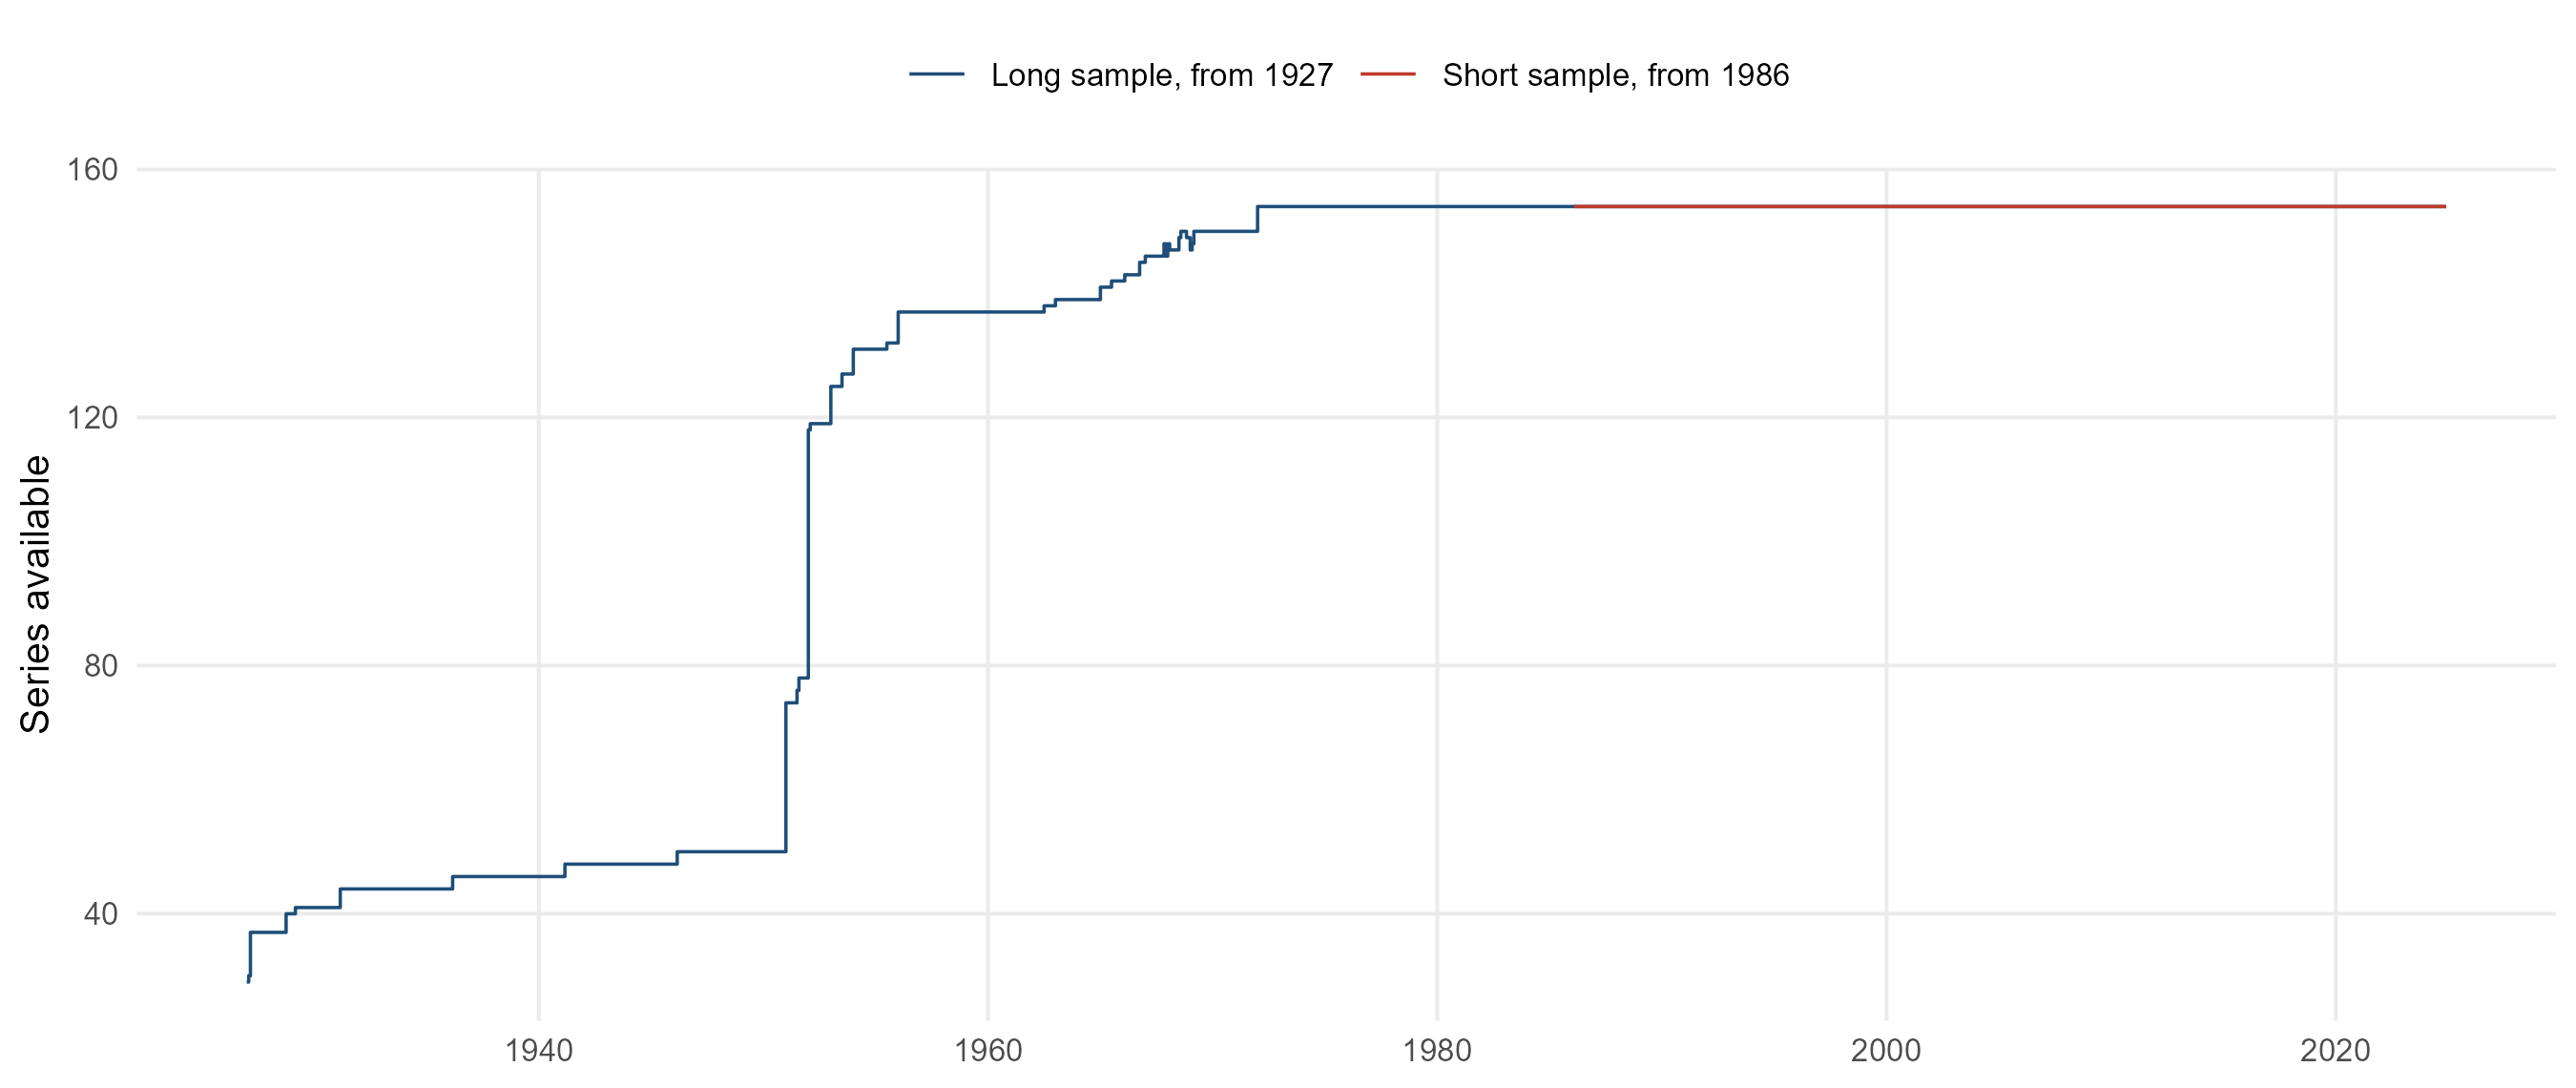
\includegraphics[width=\linewidth]{figures/data_coverage.png}
\label{fig:coverage}
\end{figure}


\begin{figure}[htbp]
\centering
\captionsetup{justification=raggedright,labelsep=none,singlelinecheck=false,labelformat=boldlabel}
\caption[Correlations among the predictors]{\footnotesize \textbf{: Correlations among the predictors.} Pairwise correlations for the market series over the common window from 1986, before preprocessing. Rows and columns are ordered by hierarchical clustering on correlation distance, so blocks of related predictors appear together.}
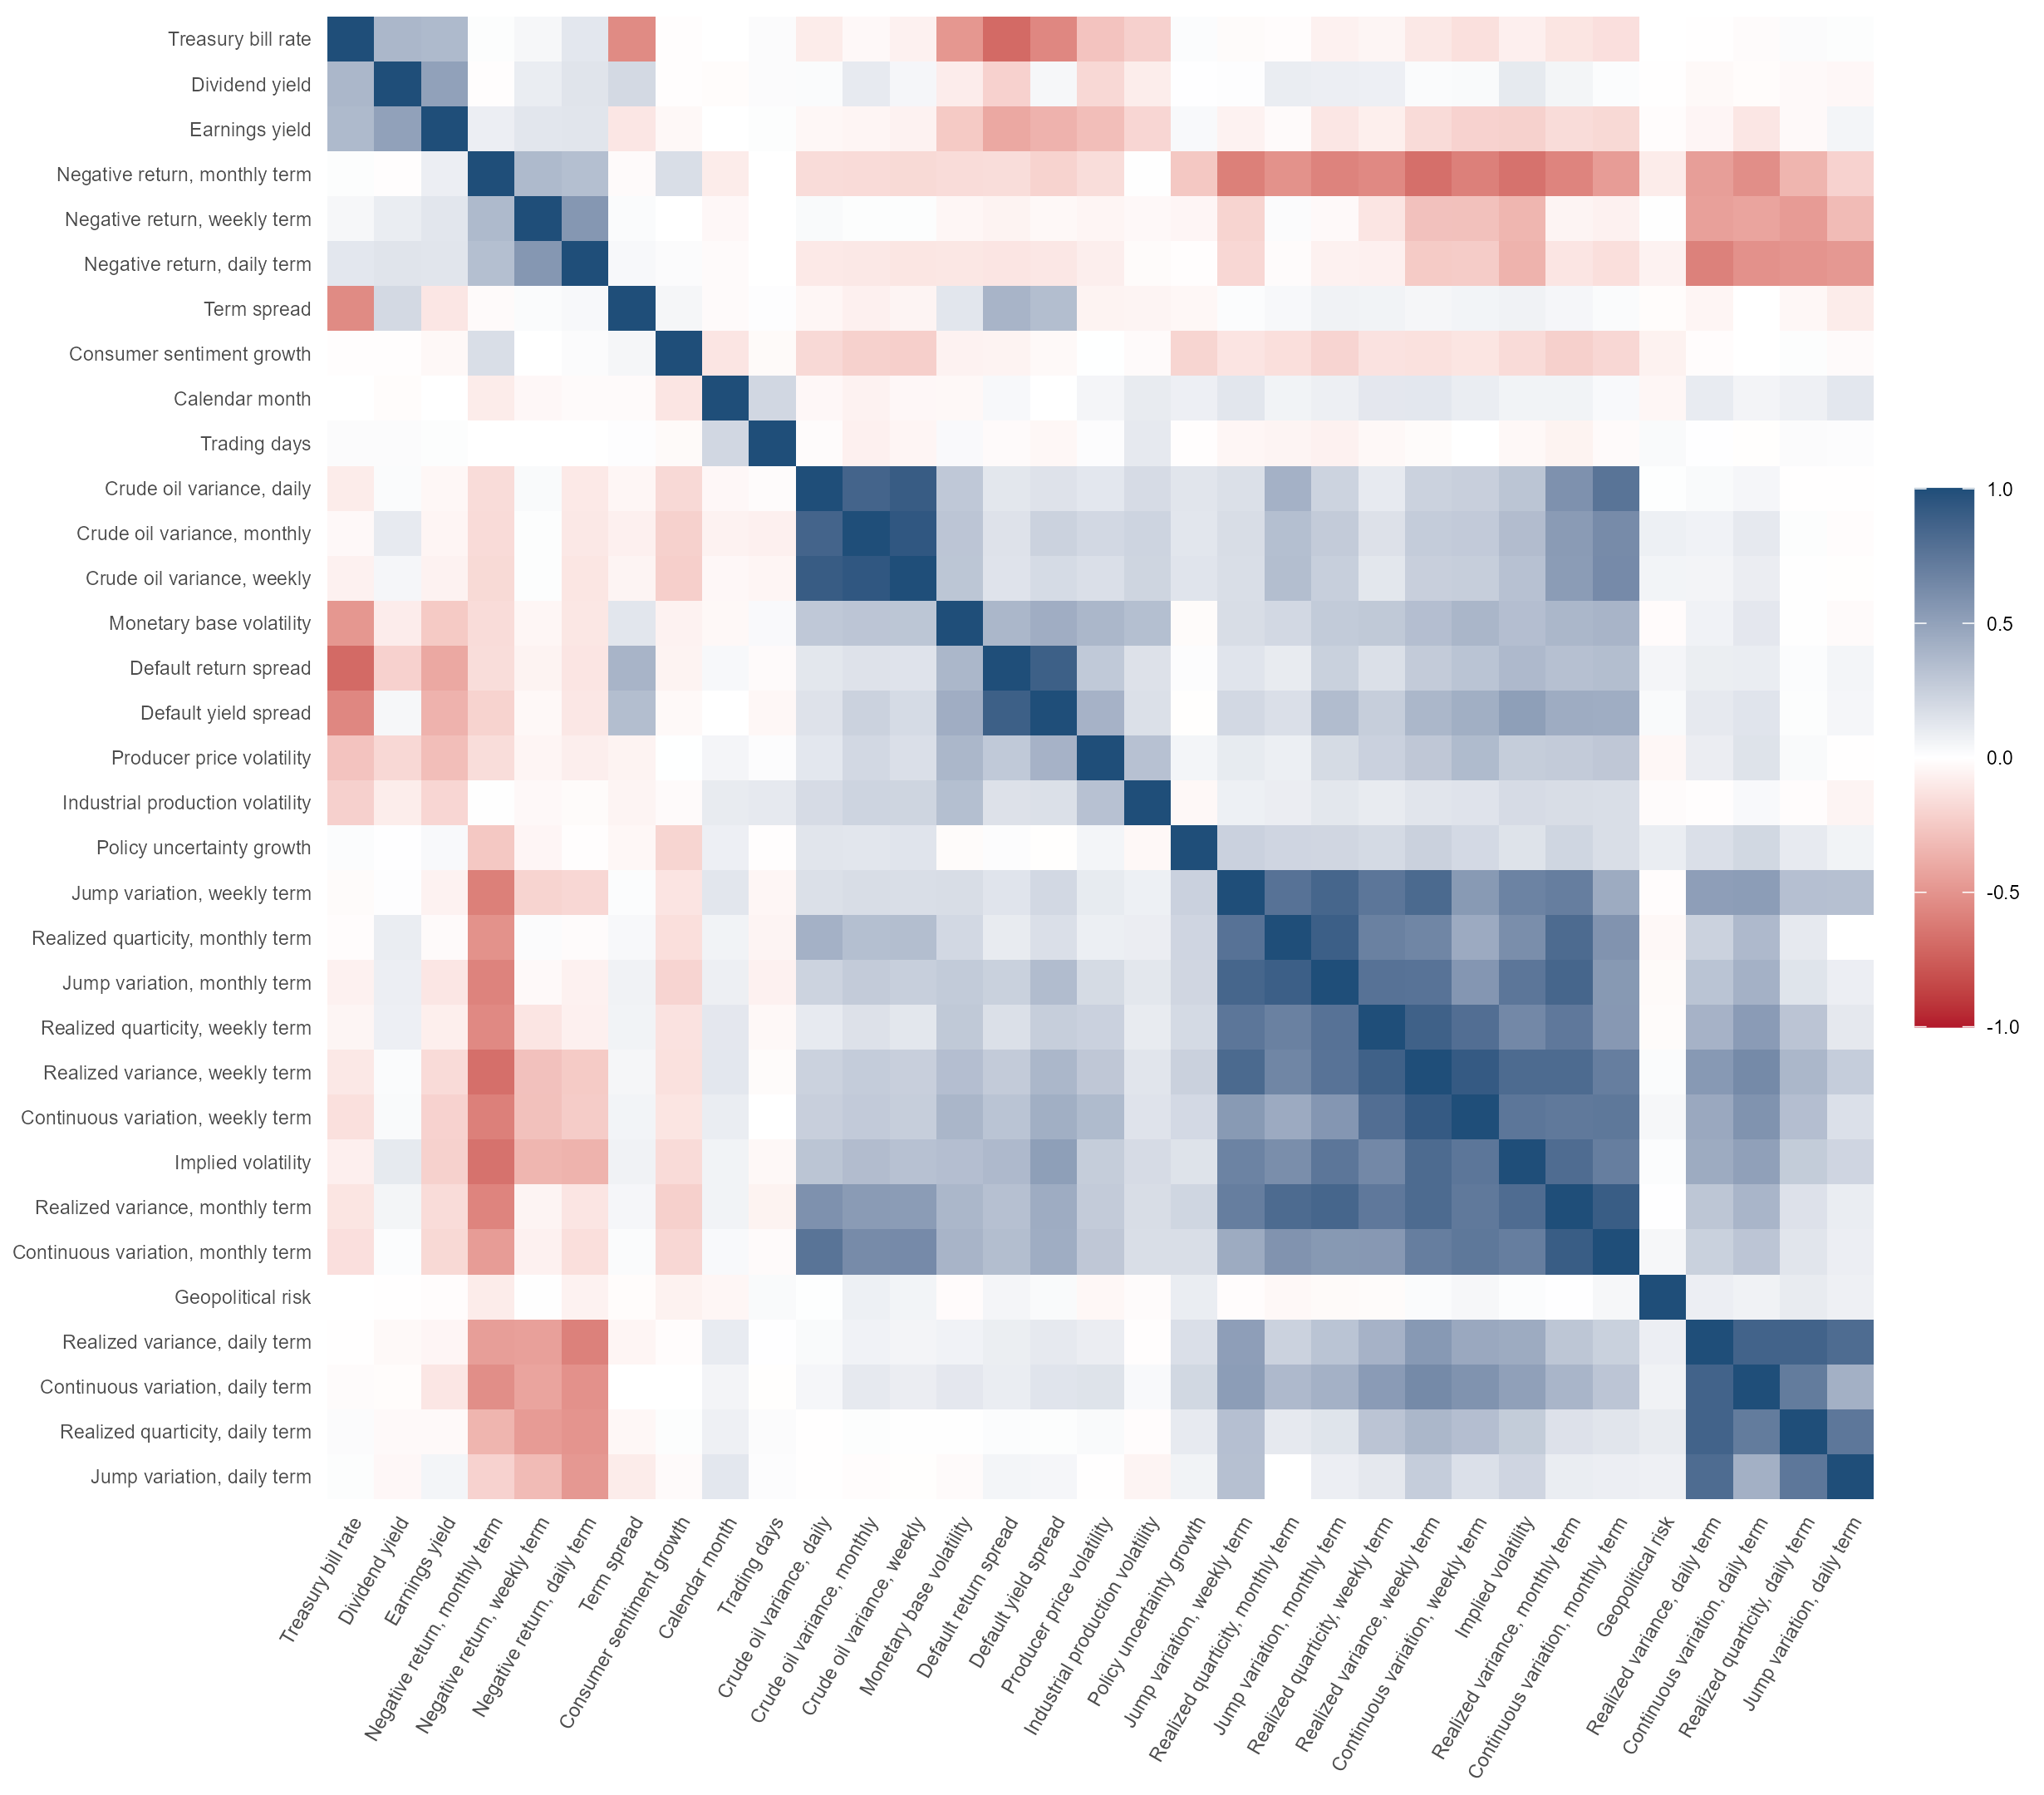
\includegraphics[width=0.92\linewidth]{figures/data_correlogram.png}
\label{fig:correlogram}
\end{figure}


\begin{figure}[htbp]
\centering
\captionsetup{justification=raggedright,labelsep=none,singlelinecheck=false,labelformat=boldlabel}
\caption[Productivity of the reviewed literature]{\footnotesize \textbf{: Productivity of the reviewed literature.} Panel (a) reports the fifteen sources publishing the most articles in the review set. Panel (b) reports the fifteen most frequent corresponding-author countries. Long source names are truncated.}
\begin{subfigure}{\linewidth}\centering
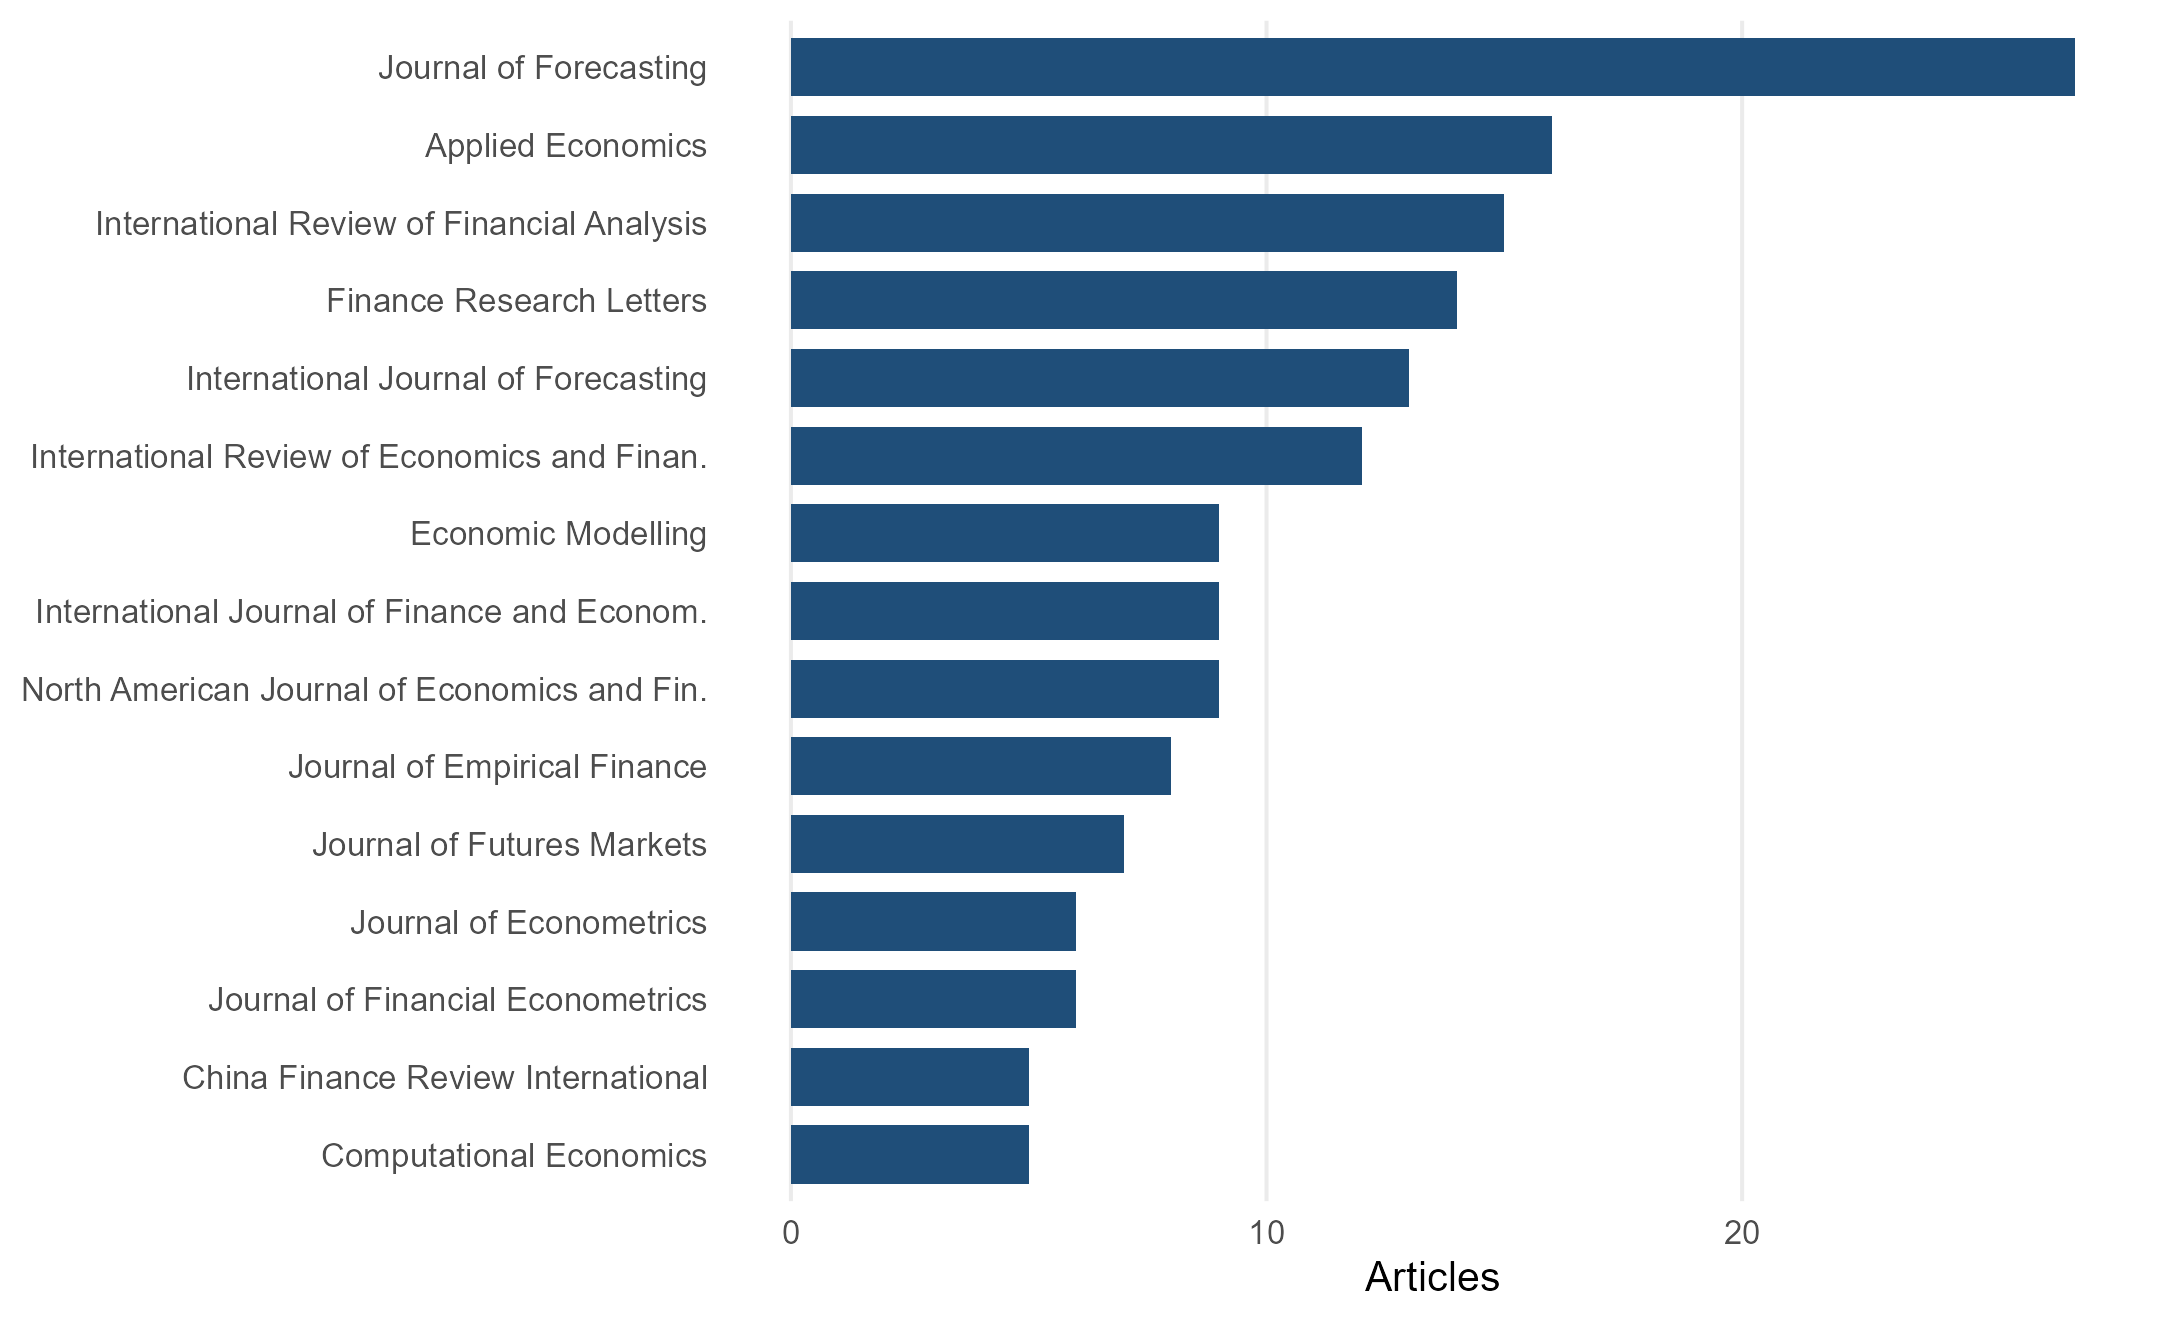
\includegraphics[width=0.86\linewidth]{figures/lit_sources.png}
\caption{Most productive sources}
\end{subfigure}
\begin{subfigure}{\linewidth}\centering
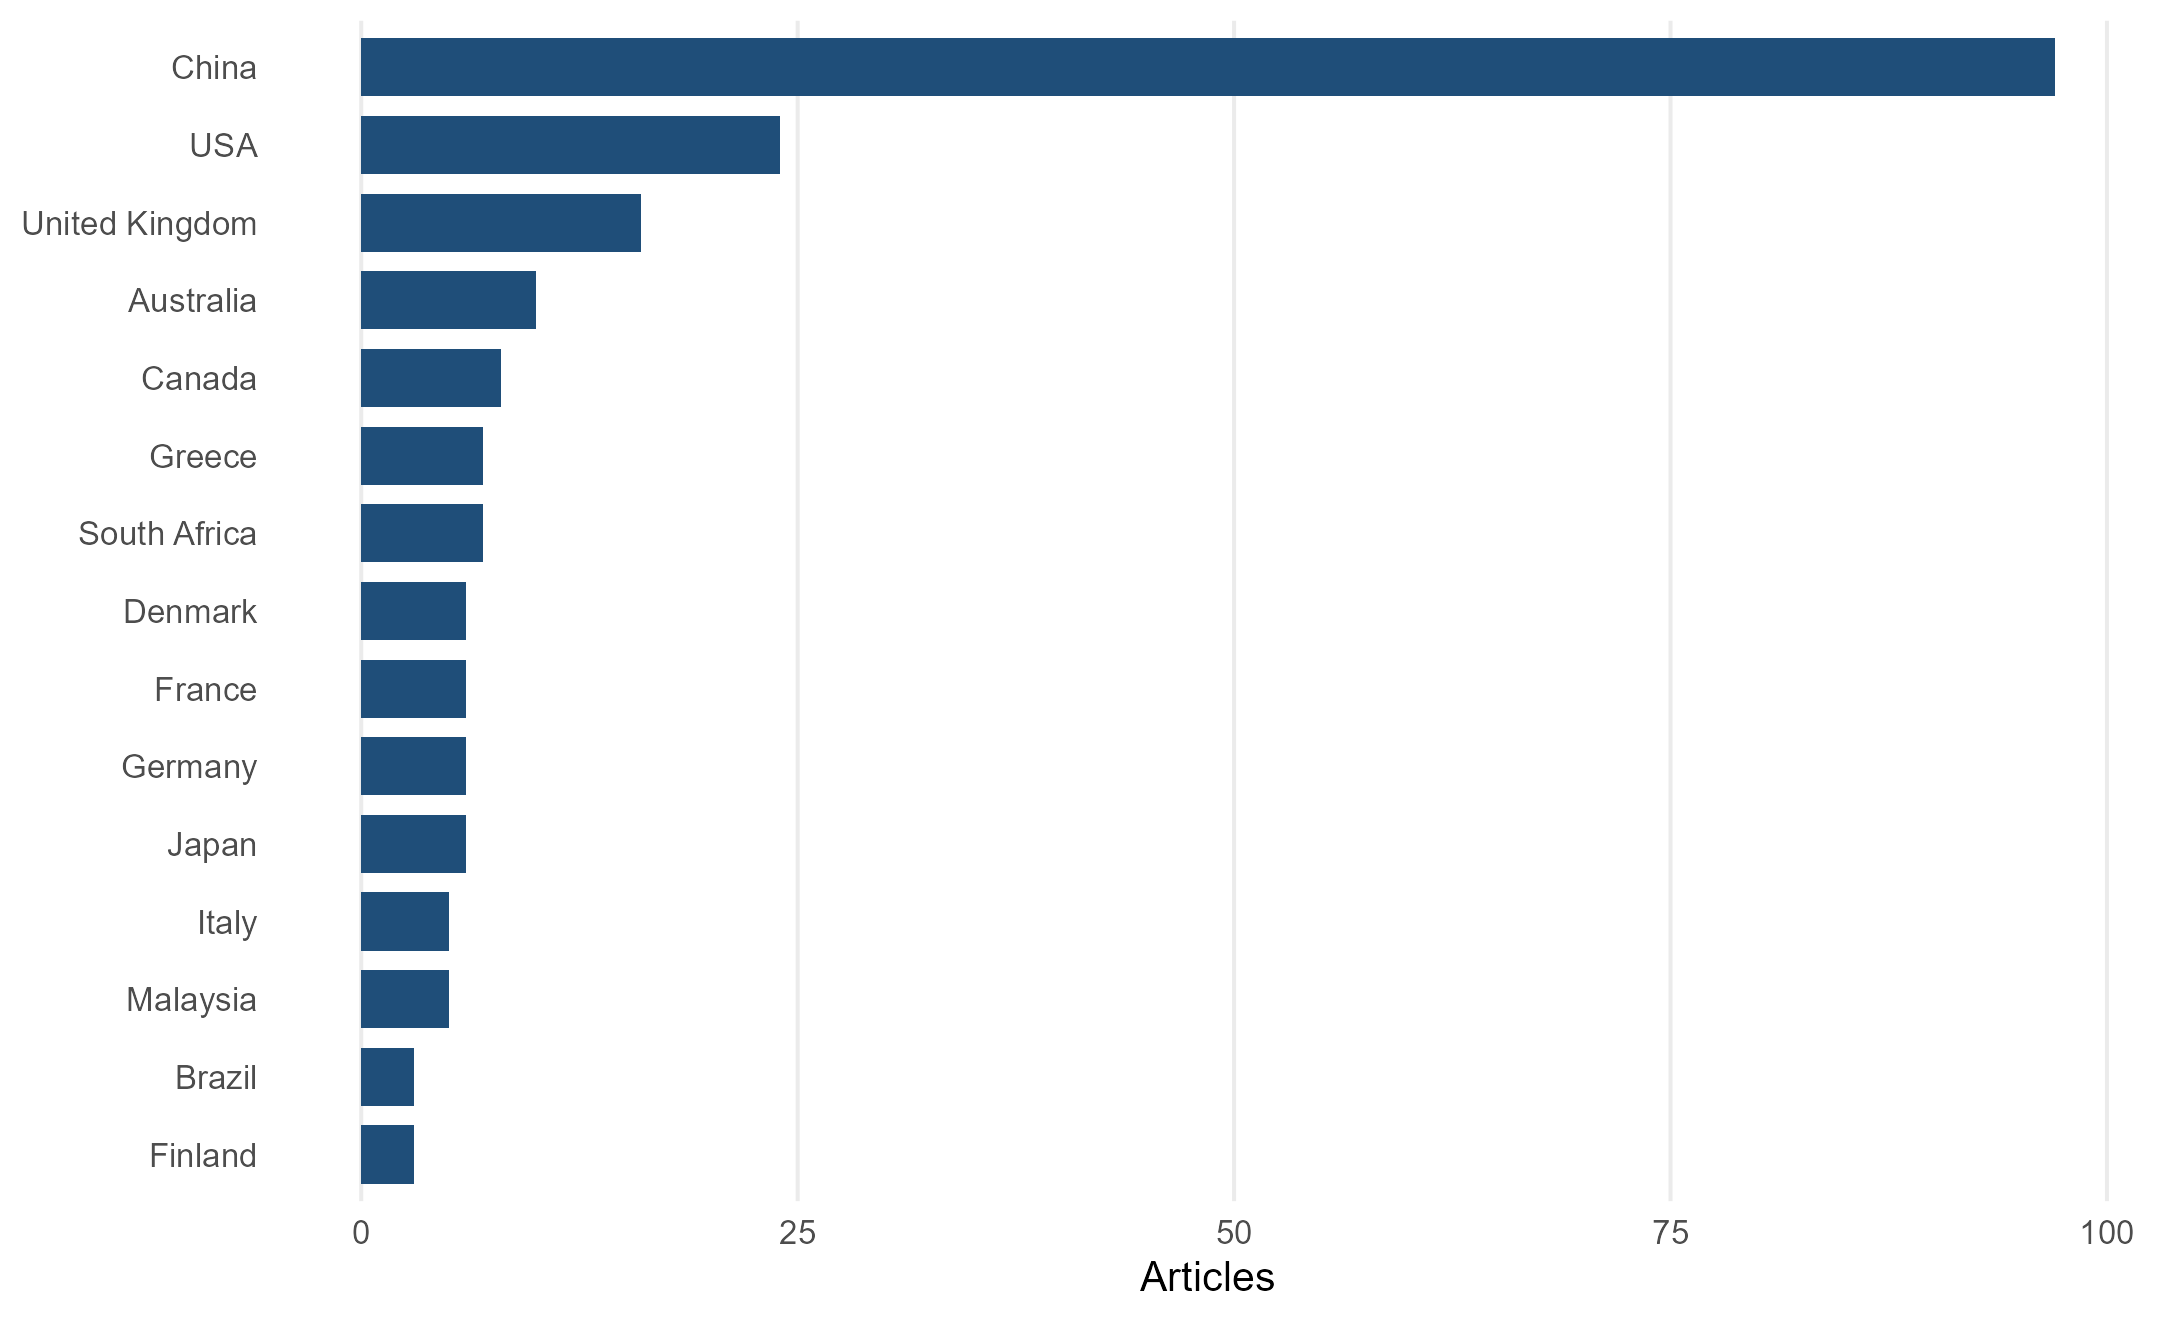
\includegraphics[width=0.86\linewidth]{figures/lit_countries.png}
\caption{Corresponding-author country}
\end{subfigure}
\label{fig:litproduction}
\end{figure}


\begin{figure}[htbp]
\centering
\captionsetup{justification=raggedright,labelsep=none,singlelinecheck=false,labelformat=boldlabel}
\caption[Intellectual and conceptual structure of the reviewed literature]{\footnotesize \textbf{: Intellectual and conceptual structure of the reviewed literature.} Panel (a) reports the fifteen references most often cited by the articles in the review set, which is the measure used in Table~\ref{tab:litfamilies}. Each bar is labelled by first author and year. The bibliographic database records the same reference with small variations in spelling, so entries are merged on a normalized key before counting; residual duplication across very similar titles by the same authors cannot be ruled out. Panel (b) is the conceptual structure map obtained by multiple correspondence analysis of the abstracts, with terms stemmed and grouped into two-word phrases and clusters assigned by $k$-means.}
\begin{subfigure}{\linewidth}\centering
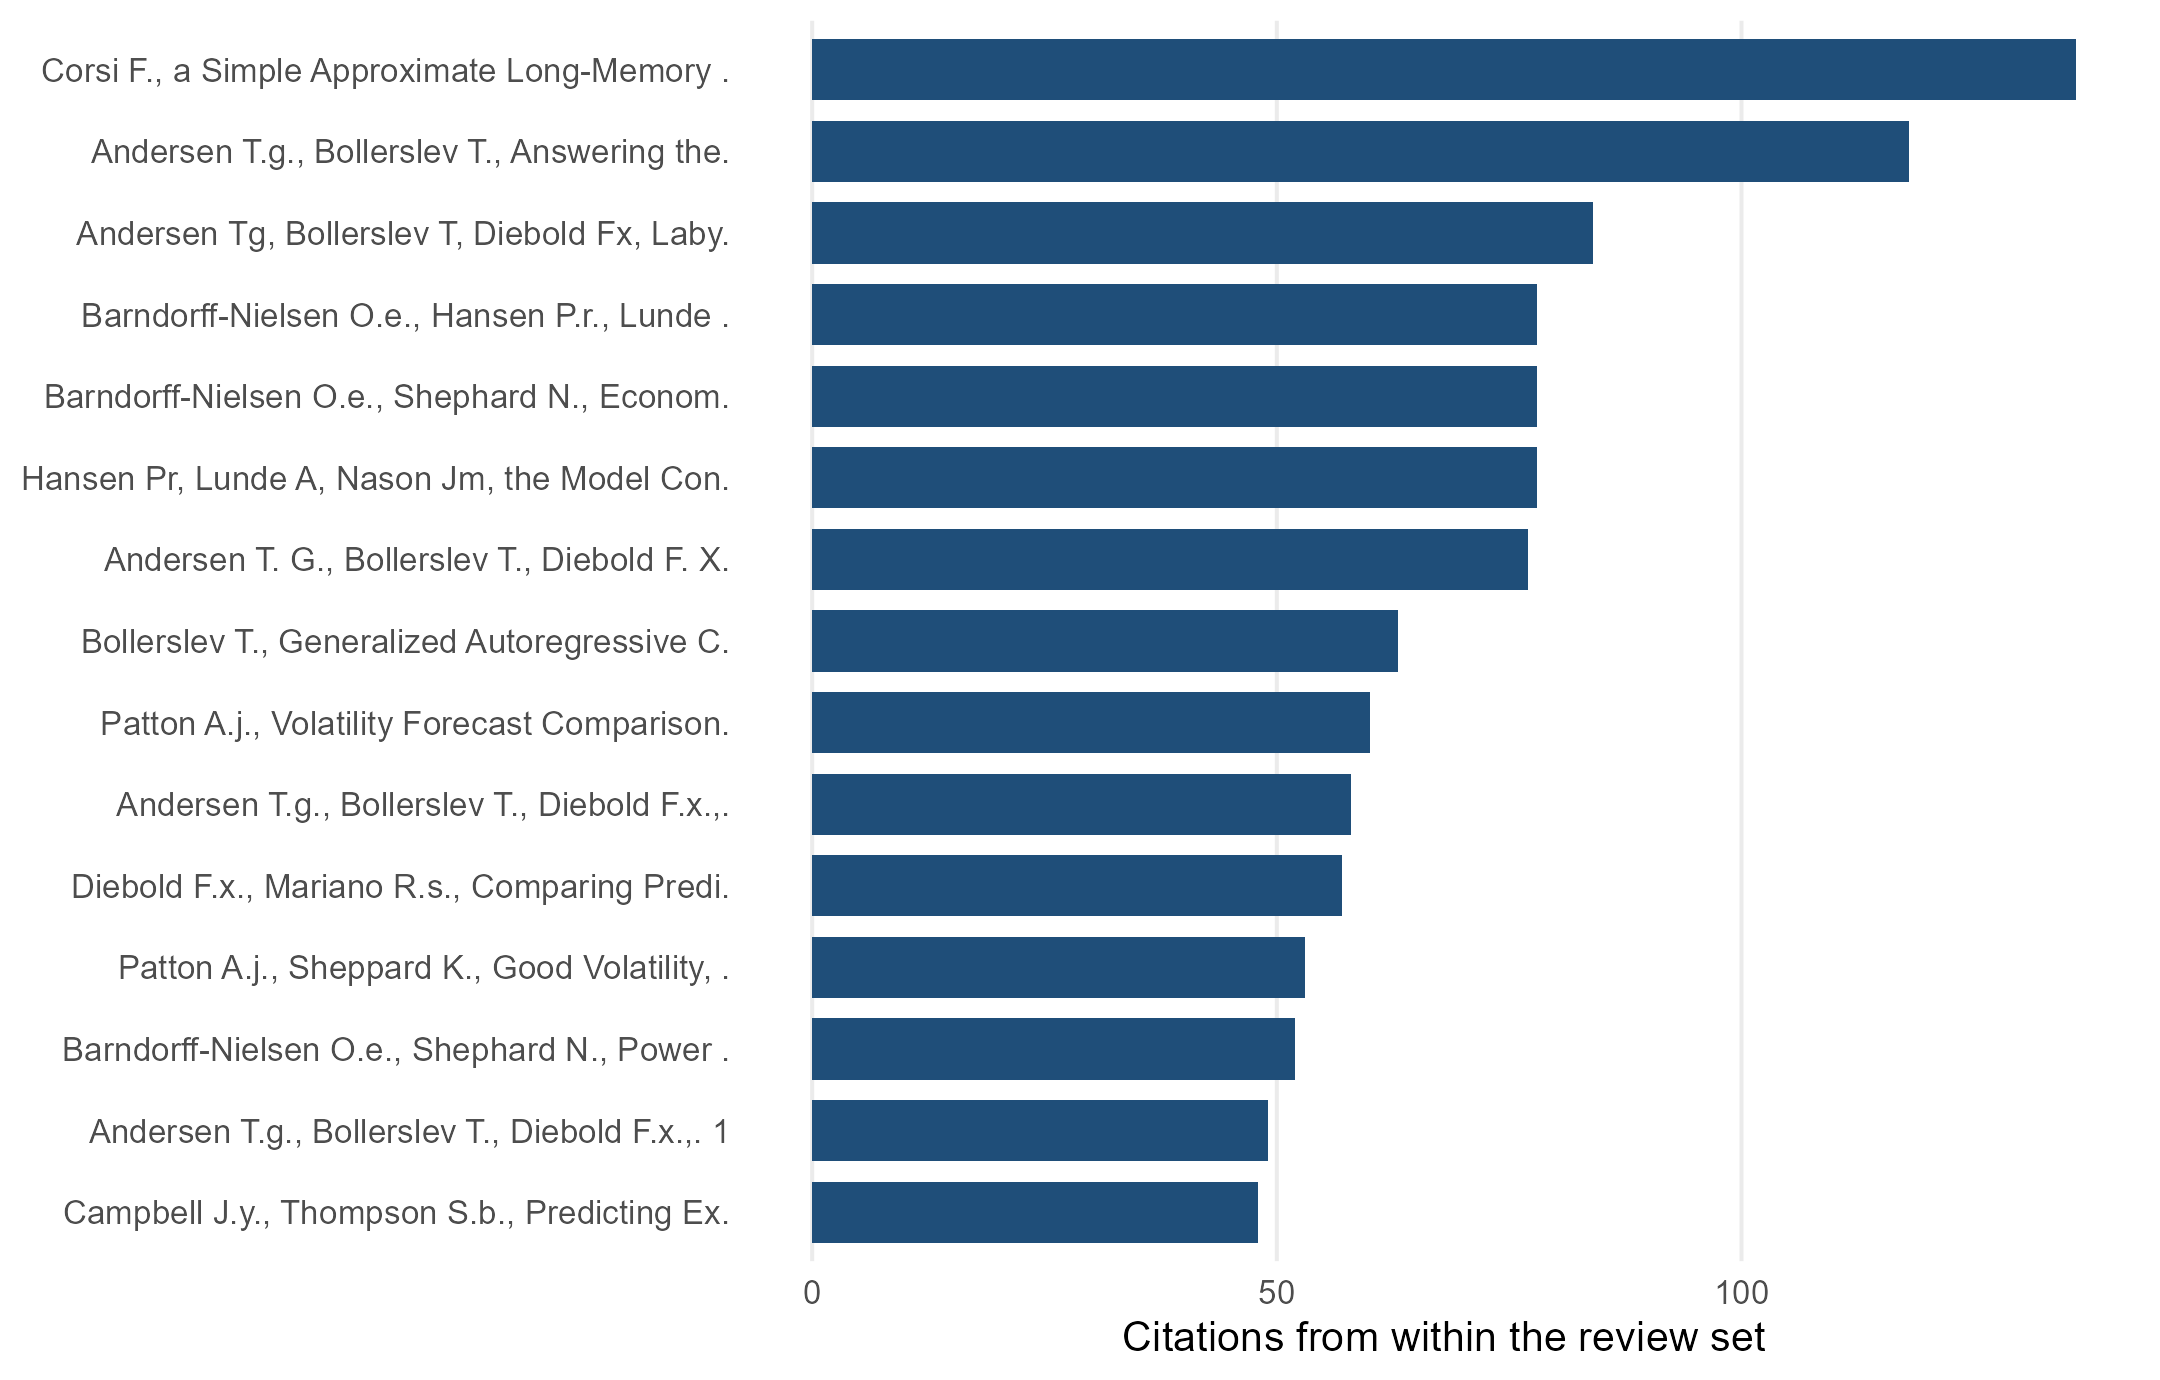
\includegraphics[width=0.86\linewidth]{figures/lit_localcited.png}
\caption{Most locally cited references}
\end{subfigure}
\begin{subfigure}{\linewidth}\centering
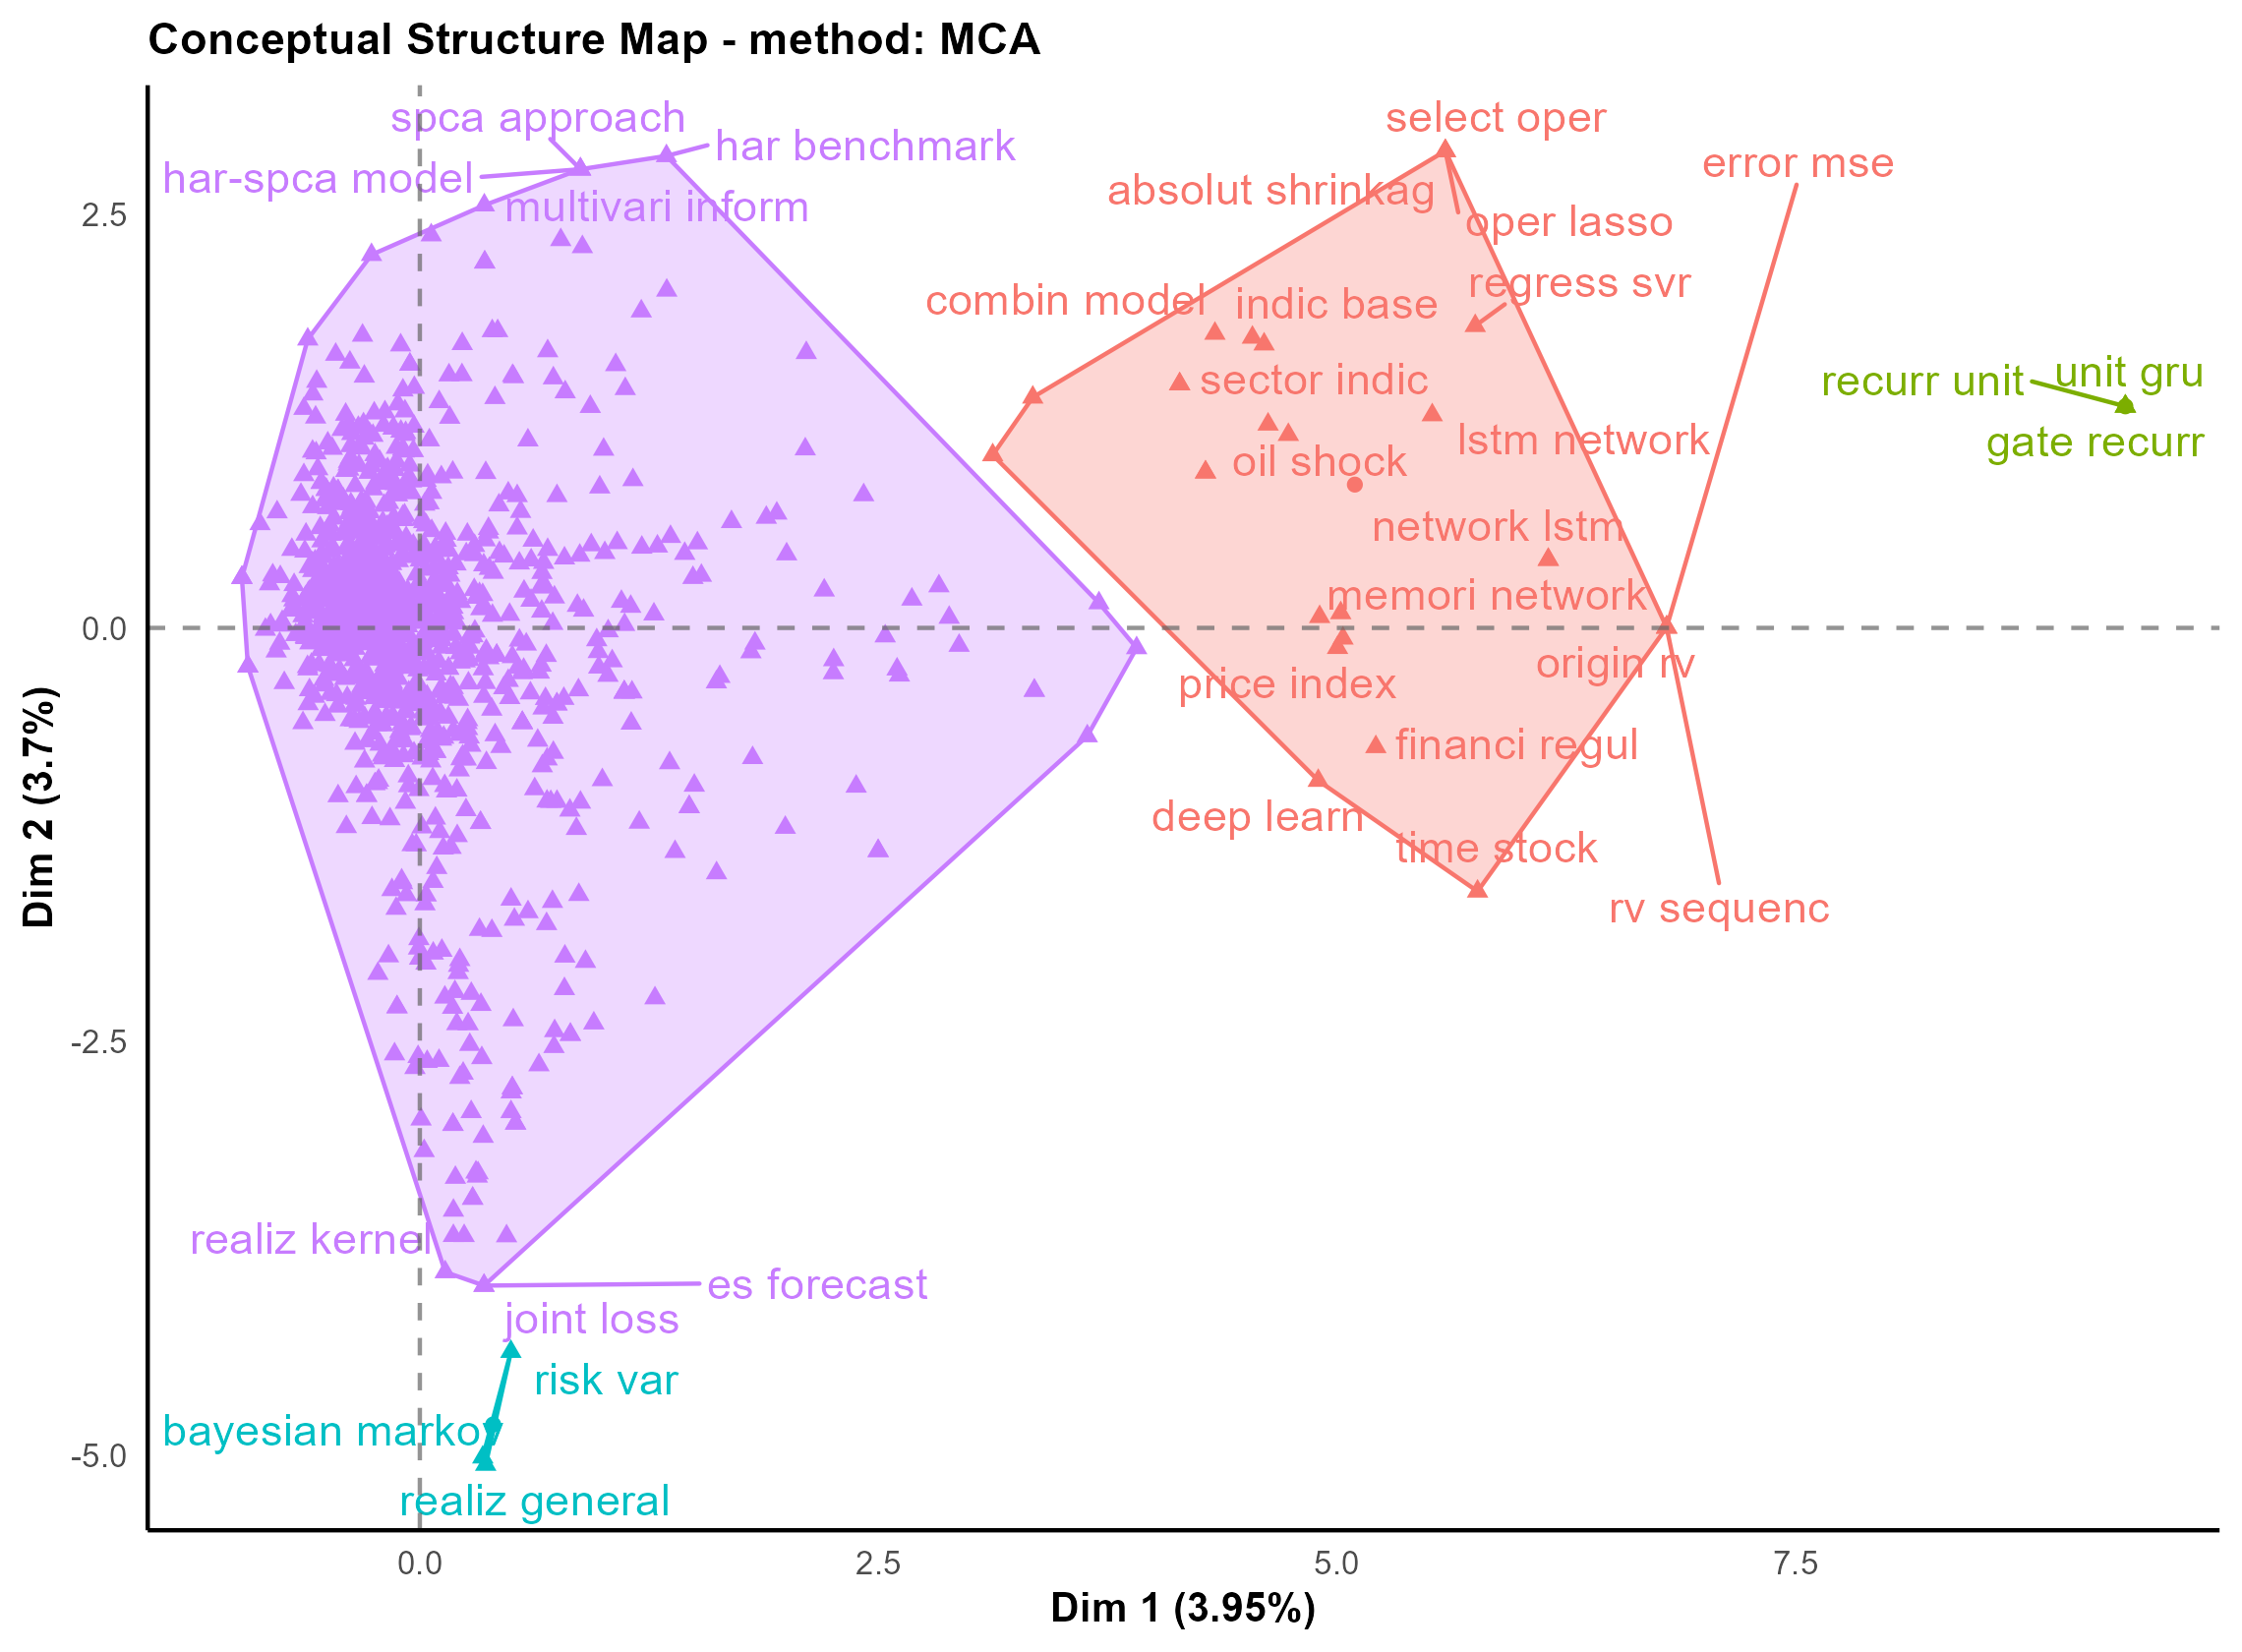
\includegraphics[width=0.72\linewidth]{figures/lit_conceptual.png}
\caption{Conceptual structure map}
\end{subfigure}
\label{fig:litstructure}
\end{figure}


\begin{figure}[htbp]
\centering
\captionsetup{justification=raggedright,labelsep=none,singlelinecheck=false,labelformat=boldlabel}
\caption[Bibliographic networks of the review corpus]{\footnotesize \textbf{: Bibliographic networks of the review corpus.} Panel (a) is the co-citation network of the 25 most co-cited references, which identifies the knowledge base the corpus draws on. Panel (b) is the keyword co-occurrence network of the 25 most frequent terms. Both use the Fruchterman-Reingold layout with Salton normalization; node size is weighted degree and edge width is tie strength.}
\begin{subfigure}{\linewidth}\centering
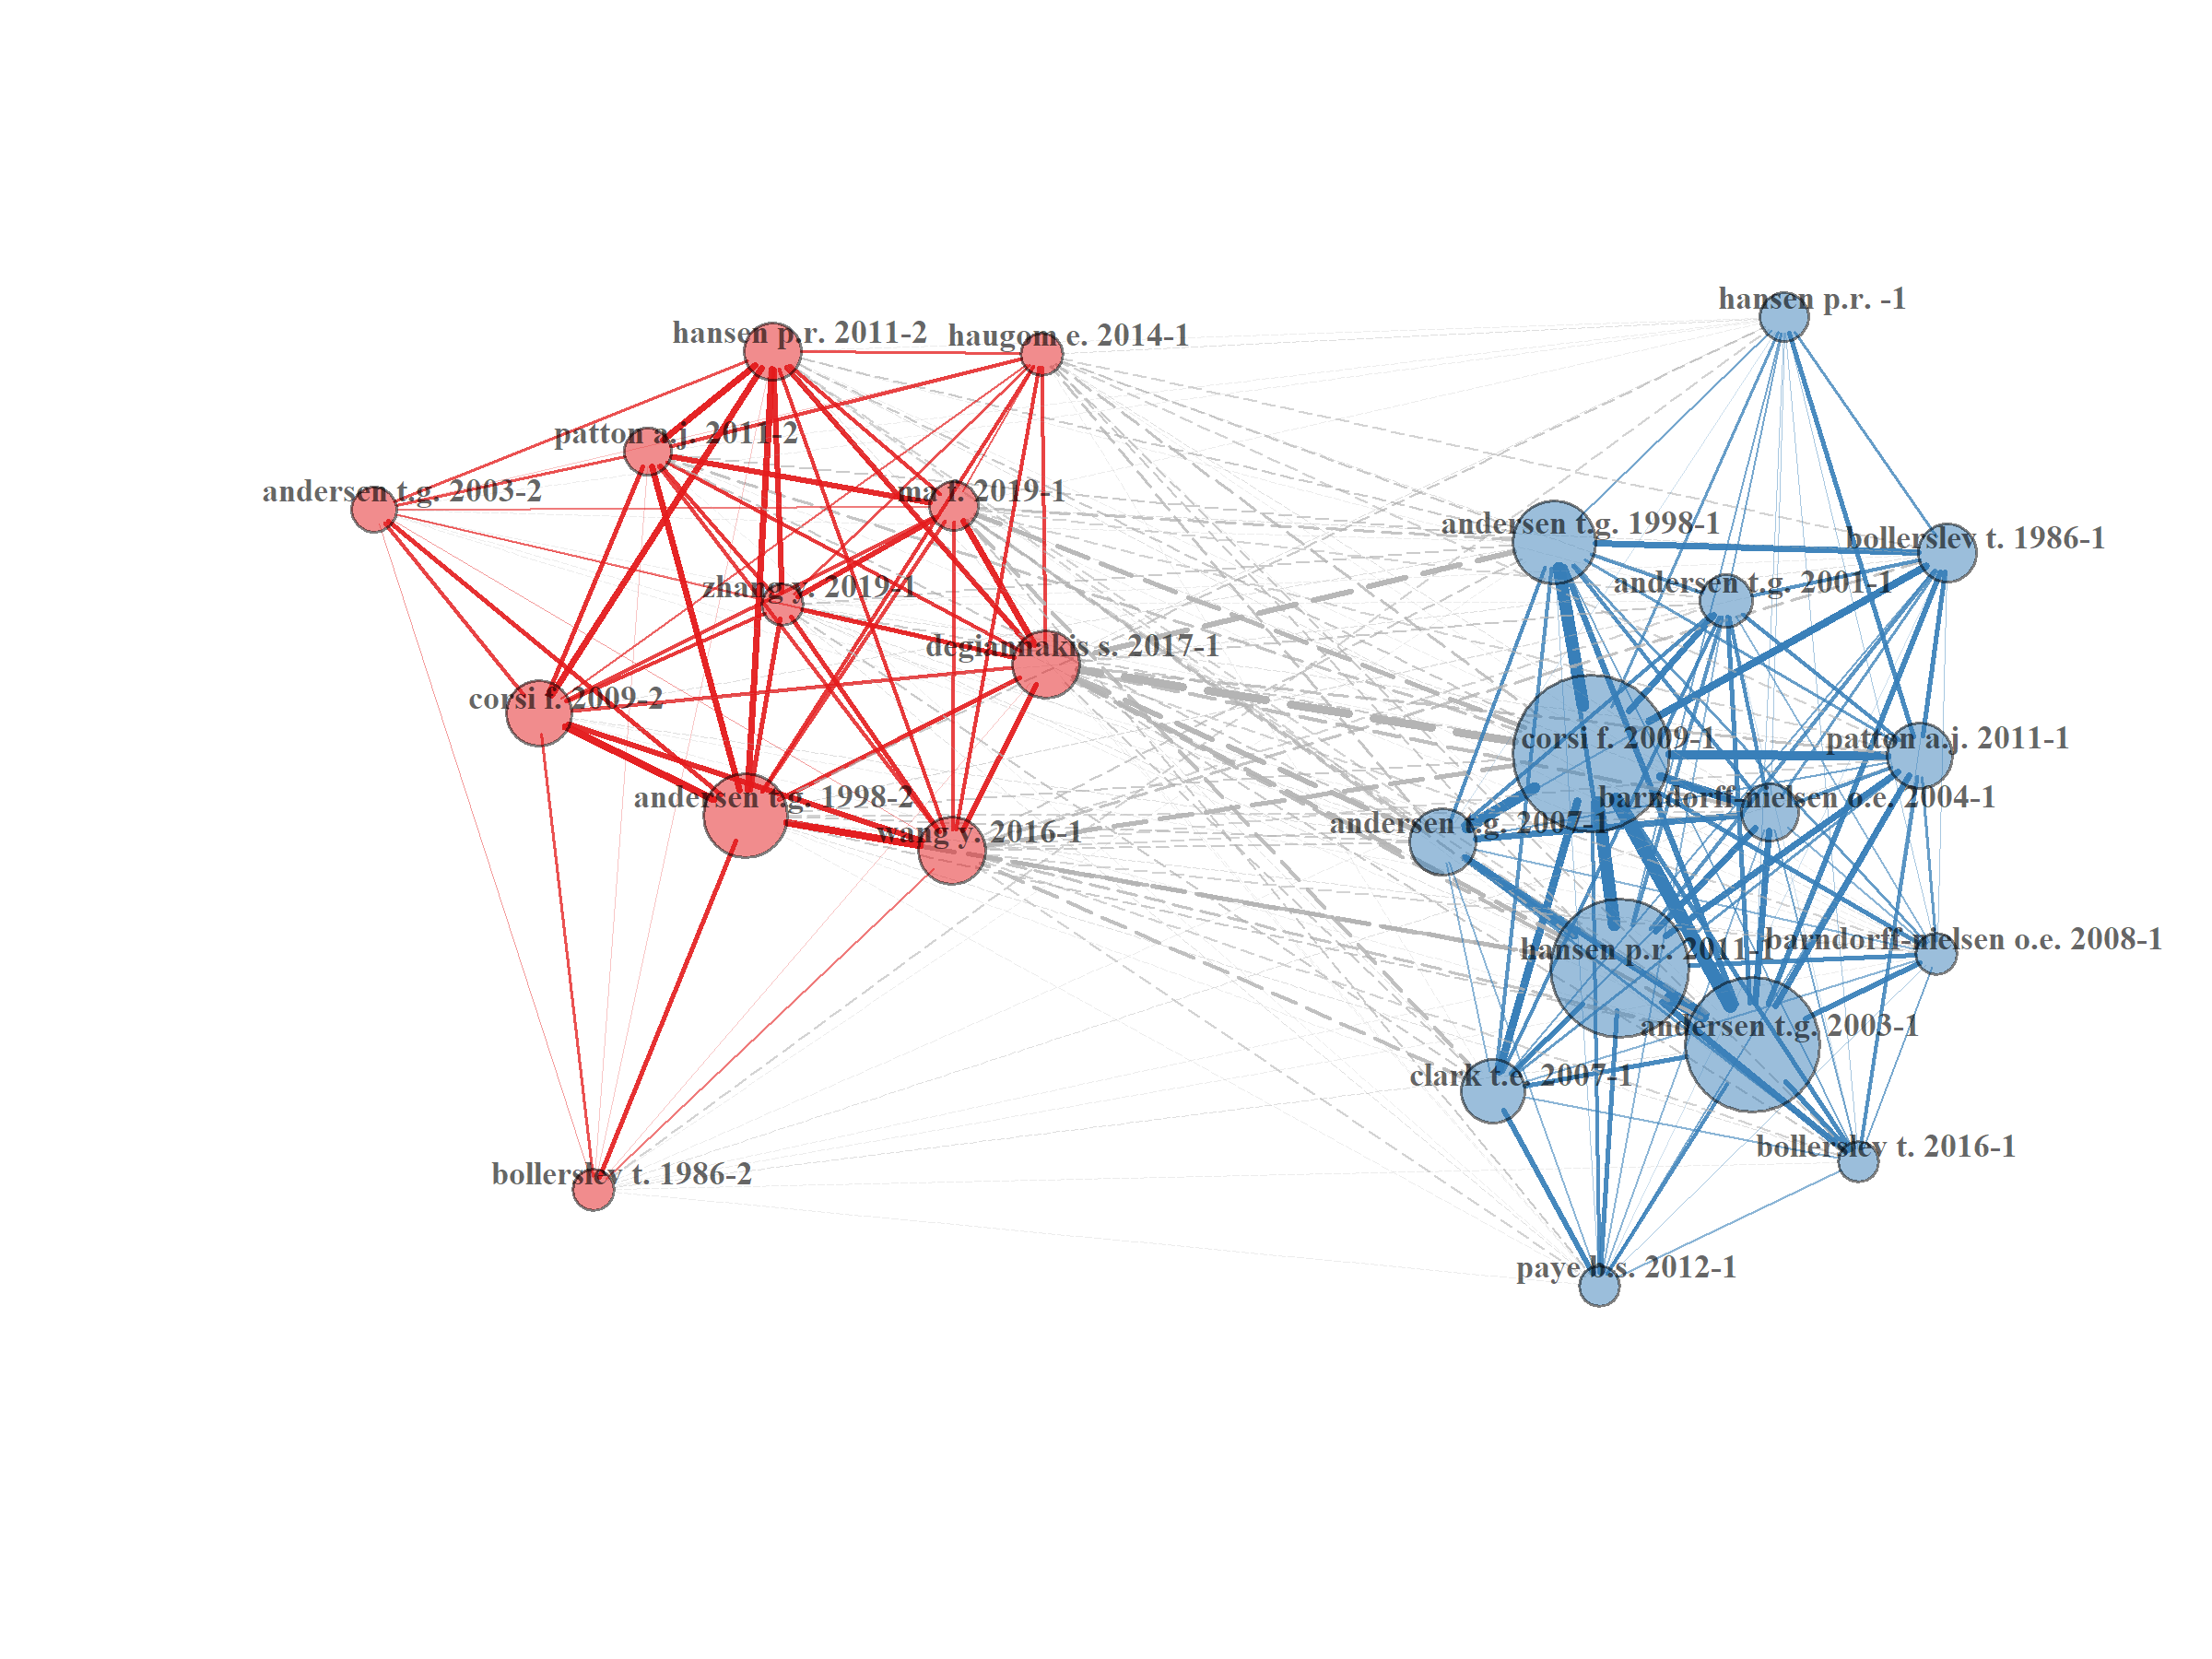
\includegraphics[width=0.86\linewidth]{figures/lit_cocitation.png}
\caption{Co-citation network}
\end{subfigure}
\begin{subfigure}{\linewidth}\centering
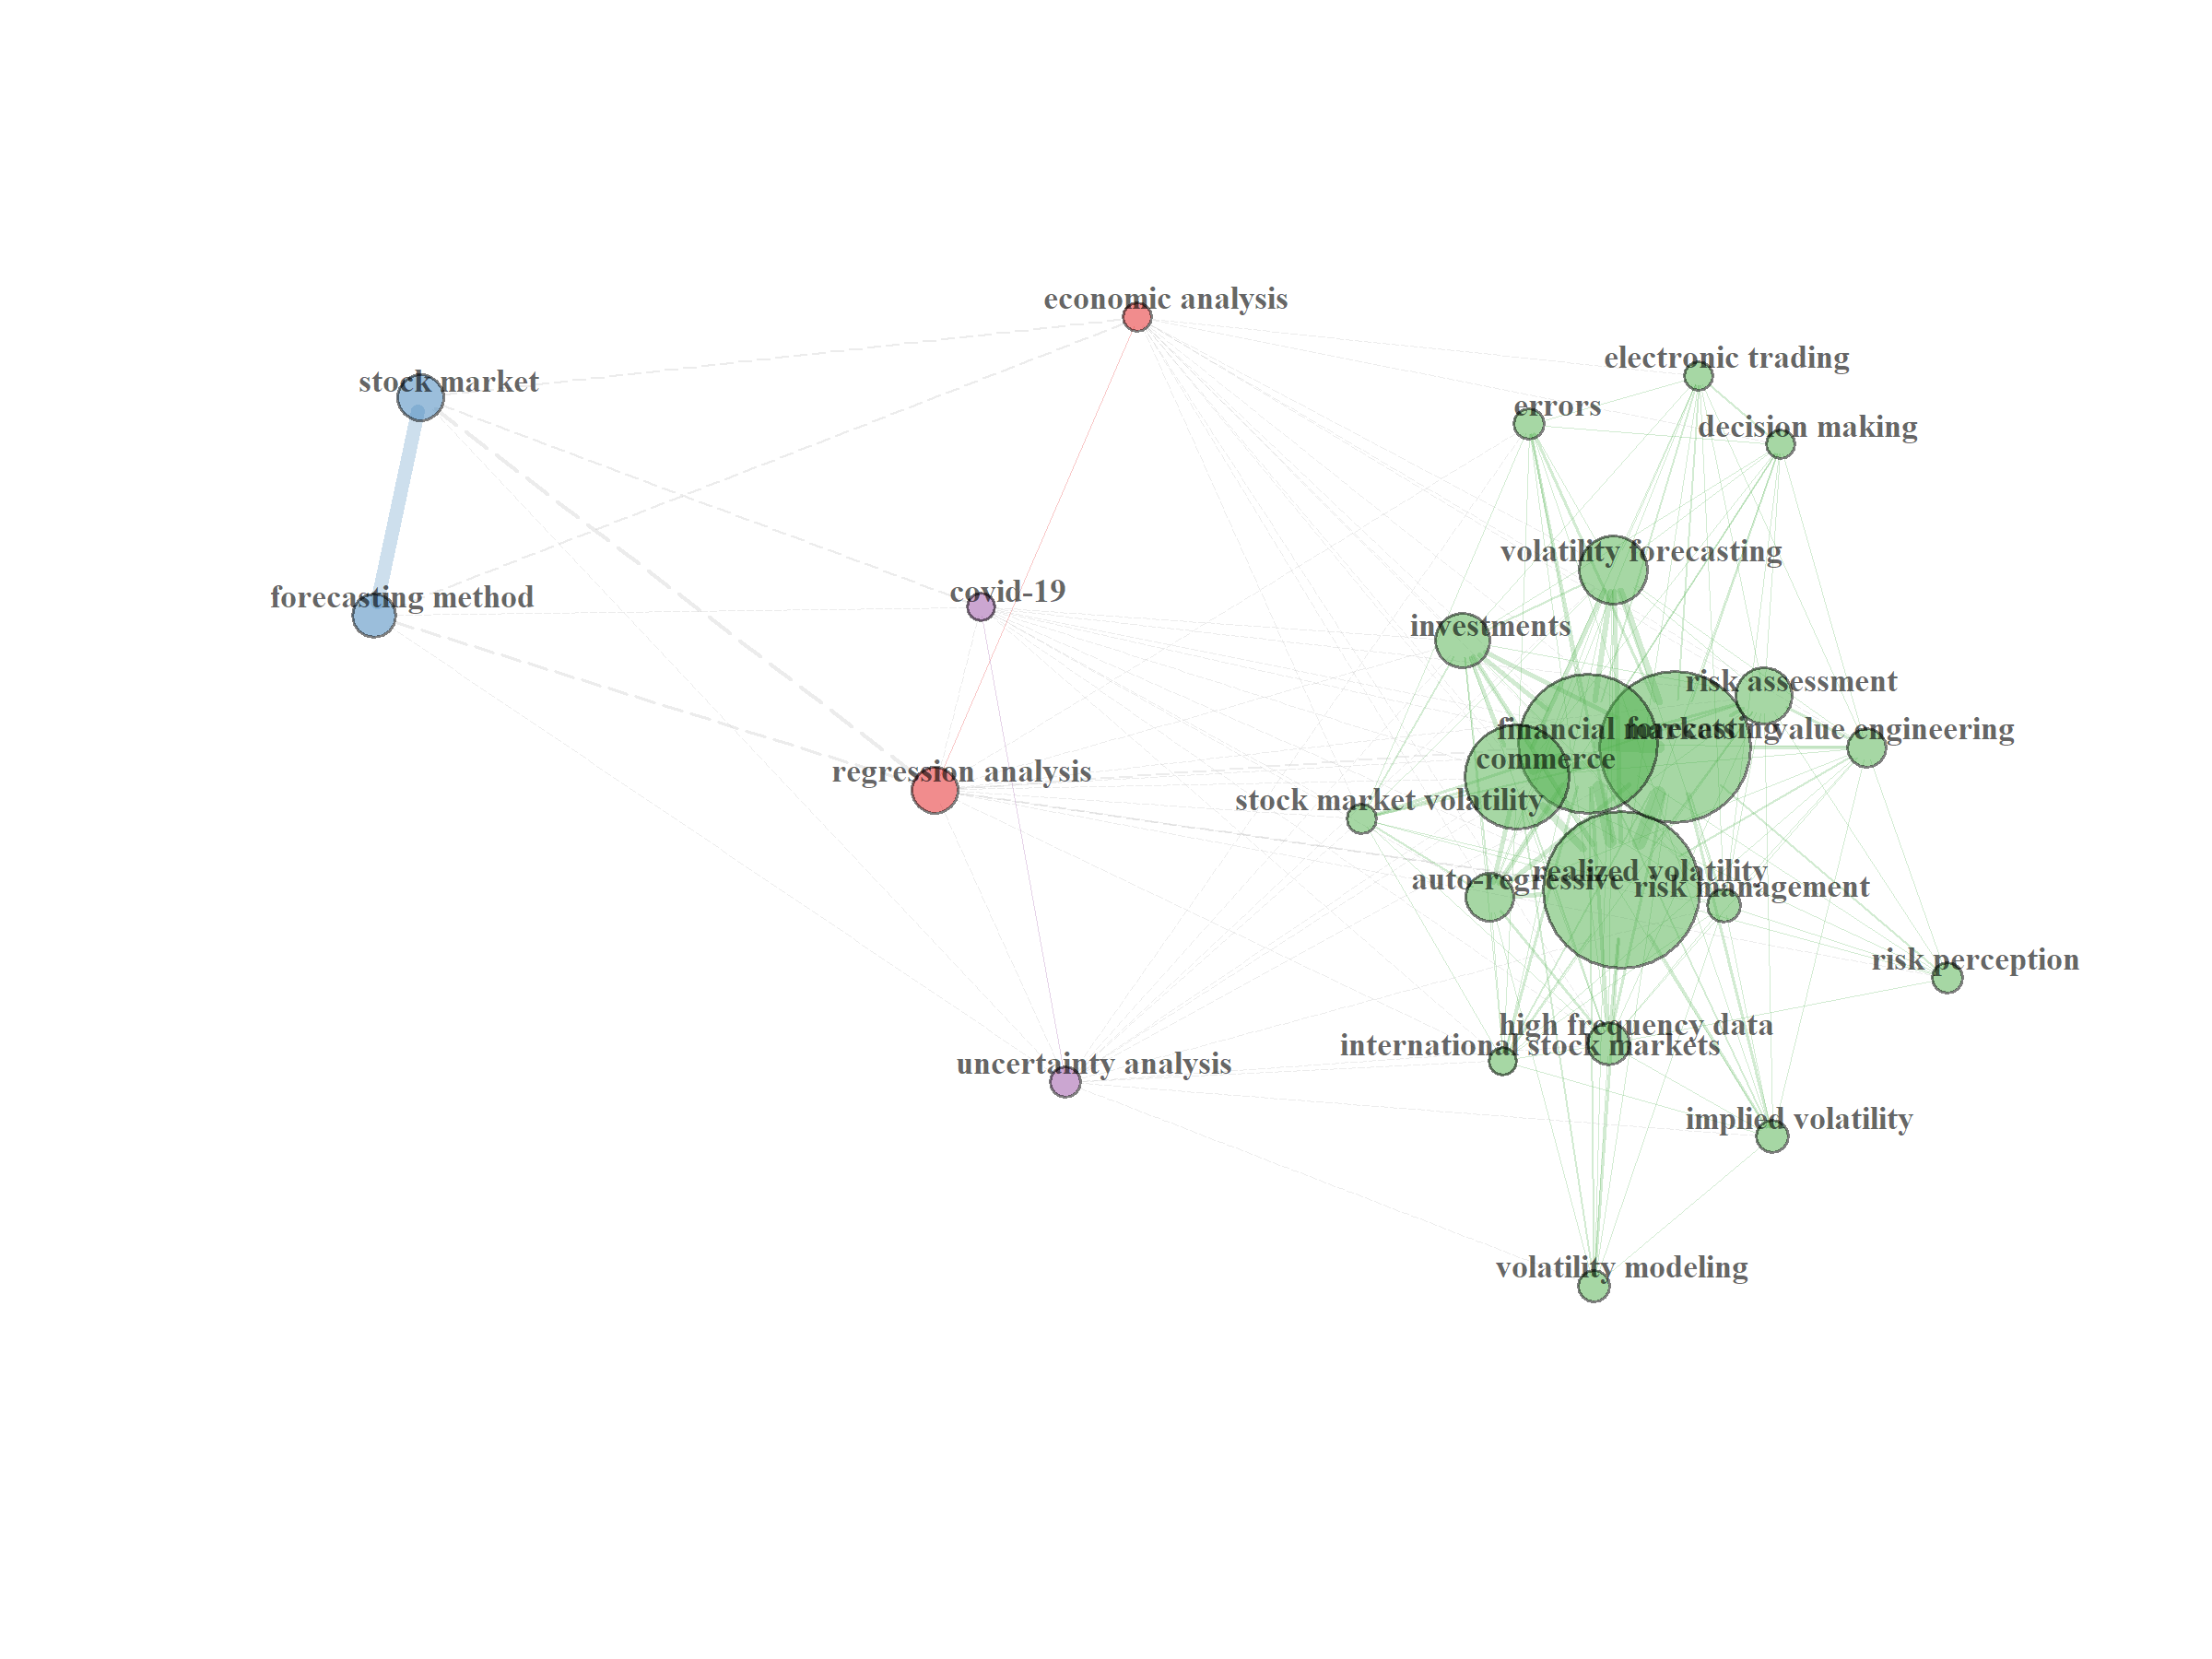
\includegraphics[width=0.86\linewidth]{figures/lit_keywords.png}
\caption{Keyword co-occurrence network}
\end{subfigure}
\label{fig:litnetworks}
\end{figure}


\begin{figure}[htbp]
\centering
\captionsetup{justification=raggedright,labelsep=none,singlelinecheck=false,labelformat=boldlabel}
\caption[Historical direct citation network]{\footnotesize \textbf{: Historical direct citation network.} Chronological map of the direct citations among the fifteen most locally cited articles in the review set. Arrows run from the citing article to the cited one, so the figure traces how the field developed in time.}
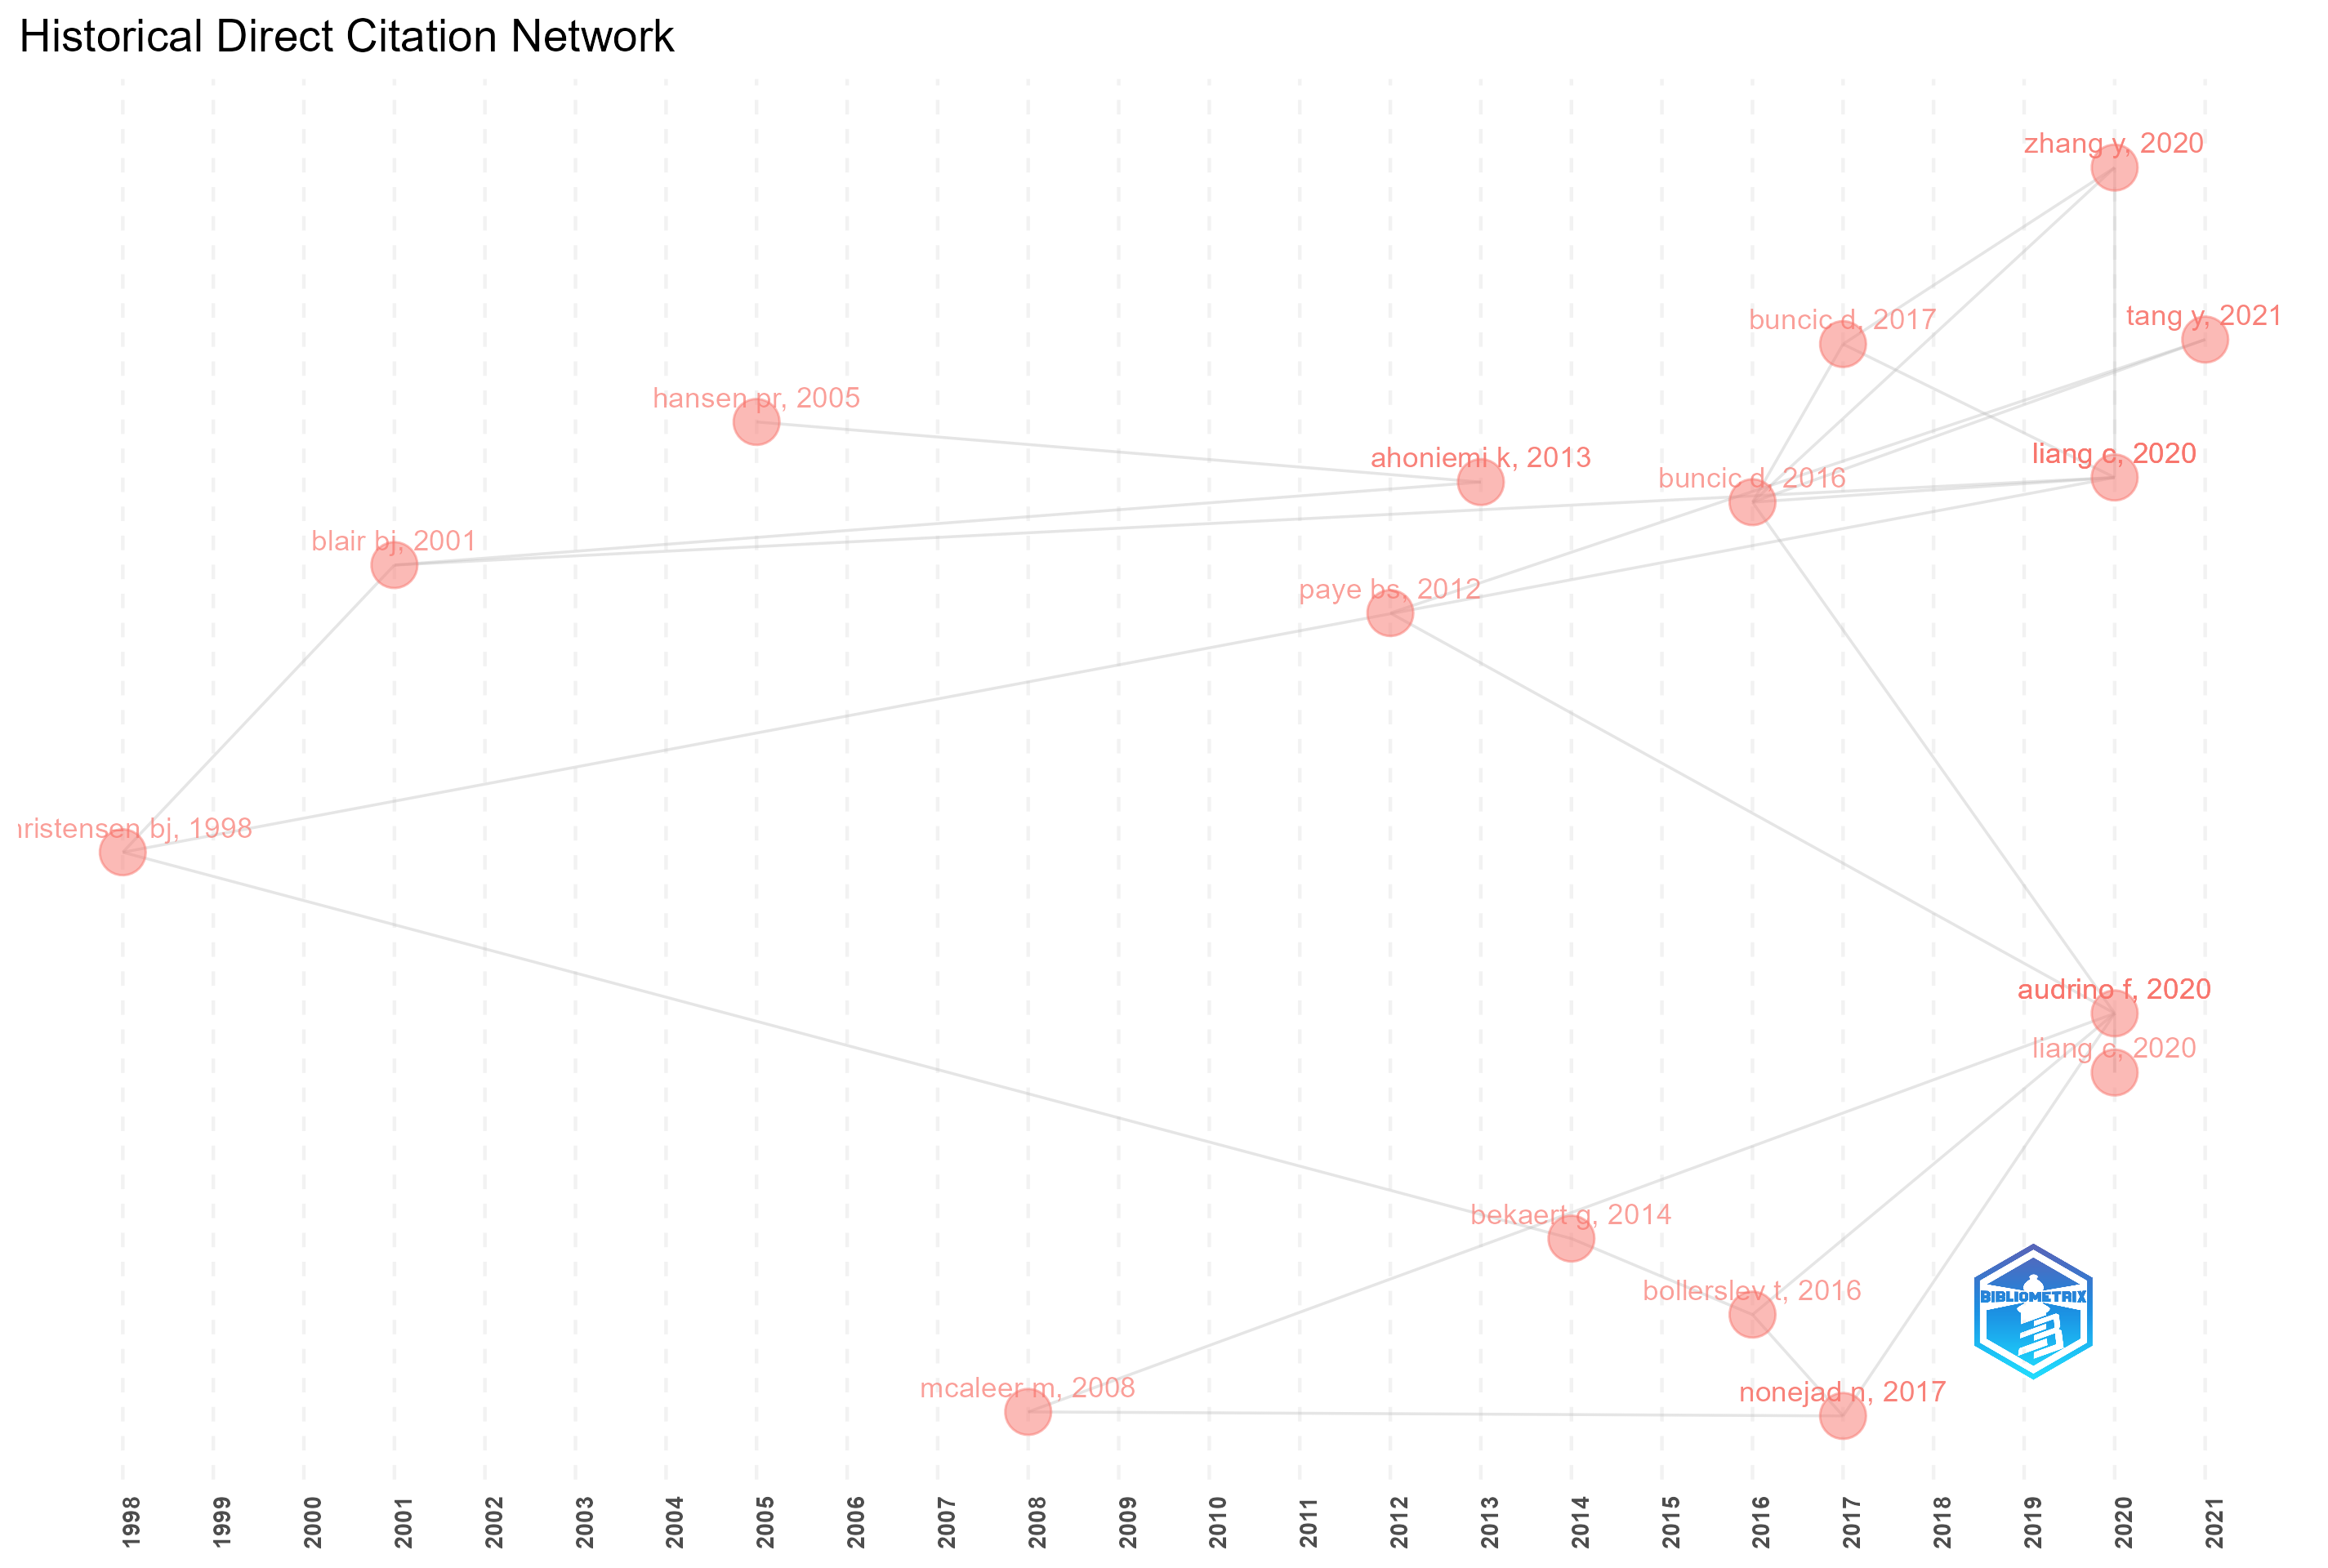
\includegraphics[width=0.98\linewidth]{figures/lit_histnetwork.png}
\label{fig:lithistnet}
\end{figure}


\begingroup\scriptsize
\captionsetup{justification=raggedright,labelsep=none,singlelinecheck=false,labelformat=boldlabel}
\setlength{\tabcolsep}{2.5pt}
\begin{longtable}{>{\raggedright\arraybackslash}p{2.6cm}rrrrrrrrr}
\caption[Out-of-sample root mean squared error by Jensen, Kelly, and Pedersen factor cluster.]{\footnotesize \textbf{: Long sample. Out-of-sample root mean squared error by Jensen, Kelly, and Pedersen factor cluster.} The first row of each panel pools all factor-month forecast errors in the cluster before computing the statistic. The remaining rows report individual factors. Light blue cells outperform HAR and bold cells identify the best model in each row. For this statistic, lower values indicate better predictive performance.}\label{tab:rv-factor_rmse}\\
\hline
Factor & HAR & HARX & ENET & RF & XGB & NN1 & NN2 & NN3 & EW \\
\hline\endfirsthead
\hline
Factor & HAR & HARX & ENET & RF & XGB & NN1 & NN2 & NN3 & EW \\
\hline\endhead
\hline\endfoot
\multicolumn{10}{@{}l}{\textit{Panel A. Accruals}} \\
\hline
Factor & HAR & HARX & ENET & RF & XGB & NN1 & NN2 & NN3 & EW \\
\hline
\textbf{Cluster aggregate} & 0.6242 & \cellcolor{blue!10}0.6129 & \cellcolor{blue!10}0.6097 & \cellcolor{blue!10}0.6098 & 0.6650 & \cellcolor{blue!10}0.6134 & \cellcolor{blue!10}0.6085 & \cellcolor{blue!10}0.6071 & \textbf{\cellcolor{blue!10}0.5977} \\
cowc\_gr1a & 0.6028 & \cellcolor{blue!10}0.5909 & \cellcolor{blue!10}0.5690 & \cellcolor{blue!10}0.5702 & 0.6230 & \cellcolor{blue!10}0.5746 & \cellcolor{blue!10}0.5722 & \cellcolor{blue!10}0.5651 & \textbf{\cellcolor{blue!10}0.5543} \\
oaccruals\_at & 0.6063 & \cellcolor{blue!10}0.5967 & \cellcolor{blue!10}0.5970 & 0.6134 & 0.6471 & \cellcolor{blue!10}0.6051 & \cellcolor{blue!10}0.6034 & \cellcolor{blue!10}0.6033 & \textbf{\cellcolor{blue!10}0.5887} \\
oaccruals\_ni & 0.6330 & \textbf{\cellcolor{blue!10}0.6140} & \cellcolor{blue!10}0.6329 & \cellcolor{blue!10}0.6151 & 0.7060 & \cellcolor{blue!10}0.6223 & \cellcolor{blue!10}0.6229 & \cellcolor{blue!10}0.6212 & \cellcolor{blue!10}0.6175 \\
seas\_16\_20na & 0.6597 & \cellcolor{blue!10}0.6464 & \cellcolor{blue!10}0.6443 & \cellcolor{blue!10}0.6257 & \cellcolor{blue!10}0.6471 & \cellcolor{blue!10}0.6440 & \cellcolor{blue!10}0.6230 & \cellcolor{blue!10}0.6233 & \textbf{\cellcolor{blue!10}0.6195} \\
taccruals\_at & 0.6232 & \cellcolor{blue!10}0.6155 & \cellcolor{blue!10}0.6006 & \cellcolor{blue!10}0.6106 & 0.6571 & \cellcolor{blue!10}0.6093 & \cellcolor{blue!10}0.6026 & \cellcolor{blue!10}0.6014 & \textbf{\cellcolor{blue!10}0.5917} \\
taccruals\_ni & 0.6157 & \cellcolor{blue!10}0.6097 & \textbf{\cellcolor{blue!10}0.6082} & 0.6210 & 0.7068 & 0.6205 & 0.6239 & 0.6250 & \cellcolor{blue!10}0.6103 \\
\hline
\multicolumn{10}{@{}l}{\textit{Panel B. Debt Issuance}} \\
\hline
Factor & HAR & HARX & ENET & RF & XGB & NN1 & NN2 & NN3 & EW \\
\hline
\textbf{Cluster aggregate} & 0.5873 & \cellcolor{blue!10}0.5746 & \cellcolor{blue!10}0.5709 & \cellcolor{blue!10}0.5859 & 0.6280 & \cellcolor{blue!10}0.5735 & 0.5878 & \cellcolor{blue!10}0.5819 & \textbf{\cellcolor{blue!10}0.5589} \\
capex\_abn & 0.6236 & \cellcolor{blue!10}0.6037 & \cellcolor{blue!10}0.5939 & \cellcolor{blue!10}0.6061 & \cellcolor{blue!10}0.5915 & \cellcolor{blue!10}0.5909 & \cellcolor{blue!10}0.5962 & \cellcolor{blue!10}0.5897 & \textbf{\cellcolor{blue!10}0.5736} \\
debt\_gr3 & 0.5491 & \cellcolor{blue!10}0.5427 & \textbf{\cellcolor{blue!10}0.5419} & 0.5757 & 0.6193 & 0.5615 & 0.5722 & 0.5704 & \cellcolor{blue!10}0.5464 \\
fnl\_gr1a & 0.5558 & \cellcolor{blue!10}0.5454 & \cellcolor{blue!10}0.5455 & 0.5596 & 0.6593 & \cellcolor{blue!10}0.5525 & 0.5790 & 0.5737 & \textbf{\cellcolor{blue!10}0.5421} \\
ncol\_gr1a & 0.6211 & \cellcolor{blue!10}0.6059 & \cellcolor{blue!10}0.6068 & \cellcolor{blue!10}0.6036 & 0.6425 & \cellcolor{blue!10}0.5926 & \cellcolor{blue!10}0.6060 & \cellcolor{blue!10}0.5947 & \textbf{\cellcolor{blue!10}0.5807} \\
nfna\_gr1a & 0.5698 & \cellcolor{blue!10}0.5521 & \cellcolor{blue!10}0.5612 & \cellcolor{blue!10}0.5537 & 0.6629 & \cellcolor{blue!10}0.5507 & 0.5758 & \cellcolor{blue!10}0.5641 & \textbf{\cellcolor{blue!10}0.5464} \\
ni\_ar1 & 0.5774 & \cellcolor{blue!10}0.5667 & \cellcolor{blue!10}0.5525 & 0.6016 & 0.6222 & \cellcolor{blue!10}0.5652 & \cellcolor{blue!10}0.5768 & \cellcolor{blue!10}0.5737 & \textbf{\cellcolor{blue!10}0.5450} \\
noa\_at & 0.6091 & \cellcolor{blue!10}0.6007 & \cellcolor{blue!10}0.5898 & \cellcolor{blue!10}0.5993 & \cellcolor{blue!10}0.5929 & \cellcolor{blue!10}0.5984 & \cellcolor{blue!10}0.6069 & \cellcolor{blue!10}0.6055 & \textbf{\cellcolor{blue!10}0.5759} \\
\hline
\multicolumn{10}{@{}l}{\textit{Panel C. Investment}} \\
\hline
Factor & HAR & HARX & ENET & RF & XGB & NN1 & NN2 & NN3 & EW \\
\hline
\textbf{Cluster aggregate} & 0.6950 & \cellcolor{blue!10}0.6869 & \cellcolor{blue!10}0.6862 & 0.7013 & 0.7255 & 0.6979 & \cellcolor{blue!10}0.6869 & \cellcolor{blue!10}0.6798 & \textbf{\cellcolor{blue!10}0.6779} \\
aliq\_at & 0.7319 & 0.7473 & 0.7412 & 0.7386 & 0.7837 & 0.7595 & \cellcolor{blue!10}0.7306 & \textbf{\cellcolor{blue!10}0.7289} & \cellcolor{blue!10}0.7317 \\
at\_gr1 & 0.7237 & \textbf{\cellcolor{blue!10}0.7209} & 0.7264 & 0.7521 & 0.7922 & 0.7382 & 0.7296 & \cellcolor{blue!10}0.7212 & \cellcolor{blue!10}0.7223 \\
be\_gr1a & 0.7167 & \cellcolor{blue!10}0.7159 & \cellcolor{blue!10}0.7128 & 0.7320 & 0.7677 & 0.7294 & \cellcolor{blue!10}0.7130 & \cellcolor{blue!10}0.7122 & \textbf{\cellcolor{blue!10}0.7100} \\
capx\_gr1 & 0.6782 & \cellcolor{blue!10}0.6692 & \cellcolor{blue!10}0.6729 & 0.7024 & 0.7163 & \cellcolor{blue!10}0.6781 & 0.6876 & \textbf{\cellcolor{blue!10}0.6645} & \cellcolor{blue!10}0.6694 \\
capx\_gr2 & 0.6307 & \cellcolor{blue!10}0.6185 & \cellcolor{blue!10}0.6176 & 0.6599 & 0.6559 & \cellcolor{blue!10}0.6281 & \cellcolor{blue!10}0.6192 & \textbf{\cellcolor{blue!10}0.6074} & \cellcolor{blue!10}0.6122 \\
capx\_gr3 & 0.7289 & \cellcolor{blue!10}0.7092 & \cellcolor{blue!10}0.6990 & 0.7365 & \cellcolor{blue!10}0.7083 & \cellcolor{blue!10}0.7170 & \cellcolor{blue!10}0.7010 & \cellcolor{blue!10}0.6963 & \textbf{\cellcolor{blue!10}0.6919} \\
coa\_gr1a & 0.6748 & 0.6766 & \cellcolor{blue!10}0.6681 & 0.6767 & 0.7115 & 0.6790 & \cellcolor{blue!10}0.6688 & \textbf{\cellcolor{blue!10}0.6584} & \cellcolor{blue!10}0.6595 \\
col\_gr1a & 0.6948 & \cellcolor{blue!10}0.6842 & \cellcolor{blue!10}0.6856 & \cellcolor{blue!10}0.6841 & 0.7359 & \cellcolor{blue!10}0.6938 & \cellcolor{blue!10}0.6780 & \textbf{\cellcolor{blue!10}0.6721} & \cellcolor{blue!10}0.6724 \\
emp\_gr1 & 0.7039 & 0.7084 & \cellcolor{blue!10}0.7022 & 0.7110 & 0.7578 & 0.7272 & 0.7084 & \cellcolor{blue!10}0.7024 & \textbf{\cellcolor{blue!10}0.6997} \\
inv\_gr1 & 0.6555 & \cellcolor{blue!10}0.6446 & \cellcolor{blue!10}0.6404 & \cellcolor{blue!10}0.6488 & 0.6745 & \cellcolor{blue!10}0.6476 & \cellcolor{blue!10}0.6365 & \textbf{\cellcolor{blue!10}0.6261} & \cellcolor{blue!10}0.6267 \\
inv\_gr1a & 0.6529 & \cellcolor{blue!10}0.6387 & \cellcolor{blue!10}0.6391 & \cellcolor{blue!10}0.6410 & 0.6820 & \cellcolor{blue!10}0.6386 & \cellcolor{blue!10}0.6330 & \textbf{\cellcolor{blue!10}0.6224} & \cellcolor{blue!10}0.6237 \\
lnoa\_gr1a & 0.6085 & \cellcolor{blue!10}0.5960 & \cellcolor{blue!10}0.5959 & \cellcolor{blue!10}0.5982 & 0.6408 & \cellcolor{blue!10}0.6011 & \cellcolor{blue!10}0.5948 & \cellcolor{blue!10}0.5846 & \textbf{\cellcolor{blue!10}0.5832} \\
mispricing\_mgmt & 0.7127 & 0.7130 & \textbf{\cellcolor{blue!10}0.7098} & 0.7605 & 0.7607 & 0.7304 & 0.7246 & 0.7171 & \cellcolor{blue!10}0.7112 \\
ncoa\_gr1a & 0.6388 & \cellcolor{blue!10}0.6244 & \cellcolor{blue!10}0.6204 & \cellcolor{blue!10}0.6294 & 0.6648 & \cellcolor{blue!10}0.6262 & \cellcolor{blue!10}0.6221 & \cellcolor{blue!10}0.6095 & \textbf{\cellcolor{blue!10}0.6064} \\
nncoa\_gr1a & 0.6360 & \cellcolor{blue!10}0.6220 & \cellcolor{blue!10}0.6205 & \cellcolor{blue!10}0.6304 & 0.6743 & \cellcolor{blue!10}0.6289 & \cellcolor{blue!10}0.6222 & \cellcolor{blue!10}0.6099 & \textbf{\cellcolor{blue!10}0.6095} \\
noa\_gr1a & 0.6584 & \cellcolor{blue!10}0.6556 & \cellcolor{blue!10}0.6578 & 0.6827 & 0.7103 & 0.6636 & \cellcolor{blue!10}0.6565 & \textbf{\cellcolor{blue!10}0.6435} & \cellcolor{blue!10}0.6515 \\
ppeinv\_gr1a & 0.6470 & \cellcolor{blue!10}0.6365 & \cellcolor{blue!10}0.6363 & 0.6753 & 0.6603 & 0.6511 & \cellcolor{blue!10}0.6437 & \cellcolor{blue!10}0.6332 & \textbf{\cellcolor{blue!10}0.6321} \\
ret\_60\_12 & 0.7819 & \cellcolor{blue!10}0.7507 & \cellcolor{blue!10}0.7596 & \textbf{\cellcolor{blue!10}0.7386} & \cellcolor{blue!10}0.7446 & \cellcolor{blue!10}0.7633 & \cellcolor{blue!10}0.7551 & \cellcolor{blue!10}0.7574 & \cellcolor{blue!10}0.7399 \\
sale\_gr1 & 0.7261 & \cellcolor{blue!10}0.7169 & \cellcolor{blue!10}0.7198 & 0.7363 & 0.7621 & 0.7293 & \cellcolor{blue!10}0.7181 & \cellcolor{blue!10}0.7147 & \textbf{\cellcolor{blue!10}0.7105} \\
sale\_gr3 & 0.6635 & 0.6657 & \textbf{\cellcolor{blue!10}0.6589} & 0.6894 & 0.7253 & 0.6884 & 0.6750 & 0.6746 & 0.6637 \\
saleq\_gr1 & 0.7654 & 0.7654 & \textbf{\cellcolor{blue!10}0.7619} & 0.7912 & 0.8299 & 0.7912 & 0.7661 & 0.7670 & 0.7675 \\
seas\_2\_5na & 0.8073 & \cellcolor{blue!10}0.7841 & \cellcolor{blue!10}0.7953 & \cellcolor{blue!10}0.7752 & \cellcolor{blue!10}0.7738 & \cellcolor{blue!10}0.7938 & \cellcolor{blue!10}0.7795 & \cellcolor{blue!10}0.7767 & \textbf{\cellcolor{blue!10}0.7701} \\
\hline
\multicolumn{10}{@{}l}{\textit{Panel D. Low Leverage}} \\
\hline
Factor & HAR & HARX & ENET & RF & XGB & NN1 & NN2 & NN3 & EW \\
\hline
\textbf{Cluster aggregate} & 0.7519 & \cellcolor{blue!10}0.7458 & \cellcolor{blue!10}0.7444 & 0.7560 & 0.7617 & 0.7555 & \cellcolor{blue!10}0.7465 & \cellcolor{blue!10}0.7417 & \textbf{\cellcolor{blue!10}0.7341} \\
age & 0.8061 & 0.8198 & \cellcolor{blue!10}0.7971 & \textbf{\cellcolor{blue!10}0.7808} & \cellcolor{blue!10}0.8031 & 0.8185 & \cellcolor{blue!10}0.8020 & \cellcolor{blue!10}0.7988 & \cellcolor{blue!10}0.7845 \\
aliq\_mat & 0.6771 & \cellcolor{blue!10}0.6515 & \cellcolor{blue!10}0.6572 & \cellcolor{blue!10}0.6732 & 0.6988 & \cellcolor{blue!10}0.6659 & \cellcolor{blue!10}0.6462 & \textbf{\cellcolor{blue!10}0.6437} & \cellcolor{blue!10}0.6455 \\
at\_be & 0.7489 & \cellcolor{blue!10}0.7348 & \cellcolor{blue!10}0.7350 & 0.7832 & 0.7505 & 0.7537 & \cellcolor{blue!10}0.7444 & \textbf{\cellcolor{blue!10}0.7313} & \cellcolor{blue!10}0.7336 \\
bidaskhl\_21d & 0.8422 & \cellcolor{blue!10}0.8360 & 0.8428 & \cellcolor{blue!10}0.8322 & \cellcolor{blue!10}0.8312 & 0.8483 & \cellcolor{blue!10}0.8301 & \cellcolor{blue!10}0.8277 & \textbf{\cellcolor{blue!10}0.8217} \\
cash\_at & 0.8462 & 0.8552 & 0.8542 & 0.9103 & 0.8677 & 0.8647 & 0.8572 & \textbf{\cellcolor{blue!10}0.8421} & 0.8505 \\
netdebt\_me & 0.7900 & 0.7993 & 0.7974 & 0.8278 & 0.8022 & 0.8037 & 0.7904 & \textbf{\cellcolor{blue!10}0.7800} & \cellcolor{blue!10}0.7857 \\
ni\_ivol & 0.6695 & \cellcolor{blue!10}0.6687 & \cellcolor{blue!10}0.6663 & 0.6795 & 0.6985 & 0.6767 & 0.6810 & 0.6814 & \textbf{\cellcolor{blue!10}0.6625} \\
rd5\_at & 0.7044 & \cellcolor{blue!10}0.6806 & \cellcolor{blue!10}0.6952 & \textbf{\cellcolor{blue!10}0.6738} & 0.7226 & 0.7082 & 0.7226 & 0.7279 & \cellcolor{blue!10}0.6863 \\
rd\_sale & 0.7440 & \cellcolor{blue!10}0.7257 & \cellcolor{blue!10}0.7286 & \textbf{\cellcolor{blue!10}0.6945} & 0.7443 & \cellcolor{blue!10}0.7234 & \cellcolor{blue!10}0.7166 & \cellcolor{blue!10}0.7164 & \cellcolor{blue!10}0.7042 \\
tangibility & 0.6699 & \cellcolor{blue!10}0.6440 & \cellcolor{blue!10}0.6419 & \cellcolor{blue!10}0.6561 & \cellcolor{blue!10}0.6430 & \cellcolor{blue!10}0.6499 & \cellcolor{blue!10}0.6495 & \cellcolor{blue!10}0.6426 & \textbf{\cellcolor{blue!10}0.6276} \\
z\_score & 0.7135 & 0.7178 & \textbf{\cellcolor{blue!10}0.7044} & 0.7337 & 0.7712 & 0.7317 & \cellcolor{blue!10}0.7112 & \cellcolor{blue!10}0.7091 & \cellcolor{blue!10}0.7087 \\
\hline
\multicolumn{10}{@{}l}{\textit{Panel E. Low Risk}} \\
\hline
Factor & HAR & HARX & ENET & RF & XGB & NN1 & NN2 & NN3 & EW \\
\hline
\textbf{Cluster aggregate} & 0.7735 & \cellcolor{blue!10}0.7694 & 0.7793 & \textbf{\cellcolor{blue!10}0.7435} & \cellcolor{blue!10}0.7555 & 0.7801 & \cellcolor{blue!10}0.7559 & \cellcolor{blue!10}0.7549 & \cellcolor{blue!10}0.7480 \\
beta\_60m & 0.7659 & \cellcolor{blue!10}0.7515 & 0.7687 & \textbf{\cellcolor{blue!10}0.7042} & \cellcolor{blue!10}0.7127 & \cellcolor{blue!10}0.7651 & \cellcolor{blue!10}0.7413 & \cellcolor{blue!10}0.7366 & \cellcolor{blue!10}0.7250 \\
beta\_dimson\_21d & 0.8860 & \cellcolor{blue!10}0.8761 & \cellcolor{blue!10}0.8778 & \cellcolor{blue!10}0.8699 & \cellcolor{blue!10}0.8548 & \cellcolor{blue!10}0.8731 & \cellcolor{blue!10}0.8440 & \textbf{\cellcolor{blue!10}0.8382} & \cellcolor{blue!10}0.8495 \\
betabab\_1260d & 0.7693 & \cellcolor{blue!10}0.7669 & 0.7893 & \textbf{\cellcolor{blue!10}0.7258} & \cellcolor{blue!10}0.7361 & 0.7877 & \cellcolor{blue!10}0.7476 & \cellcolor{blue!10}0.7504 & \cellcolor{blue!10}0.7447 \\
betadown\_252d & 0.7833 & \cellcolor{blue!10}0.7818 & 0.7980 & \textbf{\cellcolor{blue!10}0.7257} & \cellcolor{blue!10}0.7399 & 0.7858 & \cellcolor{blue!10}0.7545 & \cellcolor{blue!10}0.7544 & \cellcolor{blue!10}0.7493 \\
earnings\_variability & 0.6381 & 0.6396 & \cellcolor{blue!10}0.6283 & \cellcolor{blue!10}0.6164 & \cellcolor{blue!10}0.6326 & \cellcolor{blue!10}0.6256 & \cellcolor{blue!10}0.6200 & \cellcolor{blue!10}0.6134 & \textbf{\cellcolor{blue!10}0.6077} \\
ivol\_capm\_21d & 0.7890 & \cellcolor{blue!10}0.7874 & 0.7935 & \textbf{\cellcolor{blue!10}0.7688} & 0.7919 & 0.8034 & \cellcolor{blue!10}0.7820 & \cellcolor{blue!10}0.7796 & \cellcolor{blue!10}0.7724 \\
ivol\_capm\_252d & 0.7848 & 0.7893 & 0.7962 & \textbf{\cellcolor{blue!10}0.7526} & \cellcolor{blue!10}0.7825 & 0.7963 & \cellcolor{blue!10}0.7767 & \cellcolor{blue!10}0.7738 & \cellcolor{blue!10}0.7654 \\
ivol\_ff3\_21d & 0.8027 & \cellcolor{blue!10}0.7792 & \cellcolor{blue!10}0.7799 & \cellcolor{blue!10}0.8008 & 0.8070 & \cellcolor{blue!10}0.7773 & \textbf{\cellcolor{blue!10}0.7544} & \cellcolor{blue!10}0.7617 & \cellcolor{blue!10}0.7591 \\
ivol\_hxz4\_21d & 0.7814 & \cellcolor{blue!10}0.7610 & \cellcolor{blue!10}0.7777 & 0.7977 & 0.8097 & 0.7814 & \textbf{\cellcolor{blue!10}0.7580} & \cellcolor{blue!10}0.7630 & \cellcolor{blue!10}0.7642 \\
ocfq\_saleq\_std & 0.7017 & \cellcolor{blue!10}0.6881 & \textbf{\cellcolor{blue!10}0.6766} & 0.7055 & 0.7192 & \cellcolor{blue!10}0.6924 & \cellcolor{blue!10}0.6827 & \cellcolor{blue!10}0.6914 & \cellcolor{blue!10}0.6778 \\
rmax1\_21d & 0.8004 & \cellcolor{blue!10}0.7914 & \cellcolor{blue!10}0.8001 & \cellcolor{blue!10}0.7858 & \textbf{\cellcolor{blue!10}0.7721} & 0.8064 & \cellcolor{blue!10}0.7832 & \cellcolor{blue!10}0.7790 & \cellcolor{blue!10}0.7744 \\
rmax5\_21d & 0.8141 & \cellcolor{blue!10}0.8101 & 0.8208 & \textbf{\cellcolor{blue!10}0.7759} & \cellcolor{blue!10}0.7916 & 0.8212 & \cellcolor{blue!10}0.7929 & \cellcolor{blue!10}0.7886 & \cellcolor{blue!10}0.7868 \\
rvol\_21d & 0.7935 & 0.7938 & 0.8079 & \textbf{\cellcolor{blue!10}0.7491} & \cellcolor{blue!10}0.7650 & 0.8015 & \cellcolor{blue!10}0.7691 & \cellcolor{blue!10}0.7684 & \cellcolor{blue!10}0.7644 \\
seas\_6\_10na & 0.7030 & \cellcolor{blue!10}0.7012 & \cellcolor{blue!10}0.6970 & \cellcolor{blue!10}0.7001 & 0.7063 & 0.7169 & 0.7055 & 0.7033 & \textbf{\cellcolor{blue!10}0.6895} \\
turnover\_126d & 0.7324 & 0.7372 & 0.7512 & \textbf{\cellcolor{blue!10}0.6849} & \cellcolor{blue!10}0.6999 & 0.7426 & \cellcolor{blue!10}0.7192 & \cellcolor{blue!10}0.7194 & \cellcolor{blue!10}0.7076 \\
zero\_trades\_126d & 0.7913 & 0.7933 & 0.8135 & \textbf{\cellcolor{blue!10}0.7325} & \cellcolor{blue!10}0.7555 & 0.8185 & 0.7941 & 0.7939 & \cellcolor{blue!10}0.7727 \\
zero\_trades\_21d & 0.7499 & \cellcolor{blue!10}0.7489 & 0.7700 & \textbf{\cellcolor{blue!10}0.7023} & \cellcolor{blue!10}0.7301 & 0.7661 & \cellcolor{blue!10}0.7388 & \cellcolor{blue!10}0.7375 & \cellcolor{blue!10}0.7289 \\
zero\_trades\_252d & 0.7736 & 0.7810 & 0.7967 & \textbf{\cellcolor{blue!10}0.7442} & \cellcolor{blue!10}0.7591 & 0.8036 & 0.7773 & 0.7764 & \cellcolor{blue!10}0.7626 \\
\hline
\multicolumn{10}{@{}l}{\textit{Panel F. Momentum}} \\
\hline
Factor & HAR & HARX & ENET & RF & XGB & NN1 & NN2 & NN3 & EW \\
\hline
\textbf{Cluster aggregate} & 0.8833 & \cellcolor{blue!10}0.8639 & \cellcolor{blue!10}0.8681 & \cellcolor{blue!10}0.8532 & \cellcolor{blue!10}0.8604 & \cellcolor{blue!10}0.8652 & \cellcolor{blue!10}0.8467 & \cellcolor{blue!10}0.8458 & \textbf{\cellcolor{blue!10}0.8446} \\
prc\_highprc\_252d & 0.9099 & \cellcolor{blue!10}0.9016 & \cellcolor{blue!10}0.9066 & \cellcolor{blue!10}0.8845 & \cellcolor{blue!10}0.8960 & \cellcolor{blue!10}0.8991 & \cellcolor{blue!10}0.8691 & \textbf{\cellcolor{blue!10}0.8682} & \cellcolor{blue!10}0.8774 \\
resff3\_12\_1 & 0.7682 & \cellcolor{blue!10}0.7405 & \cellcolor{blue!10}0.7410 & \cellcolor{blue!10}0.7293 & \cellcolor{blue!10}0.7370 & \cellcolor{blue!10}0.7301 & \cellcolor{blue!10}0.7138 & \cellcolor{blue!10}0.7131 & \textbf{\cellcolor{blue!10}0.7107} \\
resff3\_6\_1 & 0.7842 & \cellcolor{blue!10}0.7390 & \cellcolor{blue!10}0.7491 & \cellcolor{blue!10}0.7394 & \cellcolor{blue!10}0.7570 & \cellcolor{blue!10}0.7437 & \cellcolor{blue!10}0.7240 & \cellcolor{blue!10}0.7300 & \textbf{\cellcolor{blue!10}0.7221} \\
ret\_12\_1 & 0.8524 & \cellcolor{blue!10}0.8331 & \cellcolor{blue!10}0.8409 & \cellcolor{blue!10}0.8325 & \cellcolor{blue!10}0.8344 & \cellcolor{blue!10}0.8419 & \cellcolor{blue!10}0.8202 & \textbf{\cellcolor{blue!10}0.8174} & \cellcolor{blue!10}0.8186 \\
ret\_3\_1 & 1.0234 & \cellcolor{blue!10}1.0024 & \cellcolor{blue!10}1.0050 & \cellcolor{blue!10}0.9964 & \cellcolor{blue!10}0.9911 & \cellcolor{blue!10}1.0033 & \cellcolor{blue!10}0.9934 & \cellcolor{blue!10}0.9960 & \textbf{\cellcolor{blue!10}0.9880} \\
ret\_6\_1 & 0.9204 & \cellcolor{blue!10}0.9108 & \cellcolor{blue!10}0.9121 & \cellcolor{blue!10}0.8926 & \cellcolor{blue!10}0.8933 & \cellcolor{blue!10}0.9129 & \cellcolor{blue!10}0.8956 & \cellcolor{blue!10}0.8936 & \textbf{\cellcolor{blue!10}0.8903} \\
ret\_9\_1 & 0.8677 & \cellcolor{blue!10}0.8488 & \cellcolor{blue!10}0.8537 & \cellcolor{blue!10}0.8343 & \cellcolor{blue!10}0.8464 & \cellcolor{blue!10}0.8527 & \cellcolor{blue!10}0.8348 & \textbf{\cellcolor{blue!10}0.8291} & \cellcolor{blue!10}0.8301 \\
seas\_1\_1na & 0.8908 & \cellcolor{blue!10}0.8758 & \cellcolor{blue!10}0.8785 & \cellcolor{blue!10}0.8604 & \cellcolor{blue!10}0.8760 & \cellcolor{blue!10}0.8775 & \cellcolor{blue!10}0.8608 & \cellcolor{blue!10}0.8583 & \textbf{\cellcolor{blue!10}0.8578} \\
\hline
\multicolumn{10}{@{}l}{\textit{Panel G. Profit Growth}} \\
\hline
Factor & HAR & HARX & ENET & RF & XGB & NN1 & NN2 & NN3 & EW \\
\hline
\textbf{Cluster aggregate} & 0.6963 & \cellcolor{blue!10}0.6833 & \cellcolor{blue!10}0.6806 & \cellcolor{blue!10}0.6823 & 0.7125 & \cellcolor{blue!10}0.6860 & \cellcolor{blue!10}0.6855 & \cellcolor{blue!10}0.6826 & \textbf{\cellcolor{blue!10}0.6688} \\
dsale\_dinv & 0.5877 & \cellcolor{blue!10}0.5682 & \cellcolor{blue!10}0.5635 & \textbf{\cellcolor{blue!10}0.5418} & 0.6432 & \cellcolor{blue!10}0.5563 & \cellcolor{blue!10}0.5583 & \cellcolor{blue!10}0.5519 & \cellcolor{blue!10}0.5431 \\
dsale\_drec & 0.6007 & \cellcolor{blue!10}0.5842 & \cellcolor{blue!10}0.5798 & \cellcolor{blue!10}0.5532 & 0.6577 & \cellcolor{blue!10}0.5635 & \cellcolor{blue!10}0.5644 & \cellcolor{blue!10}0.5668 & \textbf{\cellcolor{blue!10}0.5496} \\
dsale\_dsga & 0.6482 & \cellcolor{blue!10}0.6460 & \cellcolor{blue!10}0.6285 & \cellcolor{blue!10}0.6059 & \cellcolor{blue!10}0.6223 & \cellcolor{blue!10}0.6334 & \cellcolor{blue!10}0.6212 & \cellcolor{blue!10}0.6118 & \textbf{\cellcolor{blue!10}0.6035} \\
niq\_at\_chg1 & 0.6386 & \cellcolor{blue!10}0.6345 & \textbf{\cellcolor{blue!10}0.6345} & 0.6737 & 0.6861 & 0.6451 & 0.6477 & 0.6455 & \cellcolor{blue!10}0.6359 \\
niq\_be\_chg1 & 0.6517 & \cellcolor{blue!10}0.6502 & \textbf{\cellcolor{blue!10}0.6410} & 0.6797 & 0.6947 & 0.6615 & 0.6521 & 0.6555 & \cellcolor{blue!10}0.6470 \\
niq\_su & 0.6507 & \cellcolor{blue!10}0.6342 & \textbf{\cellcolor{blue!10}0.6308} & 0.6574 & 0.7008 & \cellcolor{blue!10}0.6494 & \cellcolor{blue!10}0.6479 & 0.6571 & \cellcolor{blue!10}0.6361 \\
ocf\_at\_chg1 & 0.5733 & \cellcolor{blue!10}0.5626 & \cellcolor{blue!10}0.5647 & 0.5884 & 0.6365 & \cellcolor{blue!10}0.5697 & 0.5993 & 0.5892 & \textbf{\cellcolor{blue!10}0.5609} \\
ret\_12\_7 & 0.8747 & \cellcolor{blue!10}0.8583 & \cellcolor{blue!10}0.8607 & \textbf{\cellcolor{blue!10}0.8208} & \cellcolor{blue!10}0.8319 & \cellcolor{blue!10}0.8631 & \cellcolor{blue!10}0.8580 & \cellcolor{blue!10}0.8577 & \cellcolor{blue!10}0.8379 \\
sale\_emp\_gr1 & 0.6027 & \cellcolor{blue!10}0.5832 & \cellcolor{blue!10}0.5793 & \cellcolor{blue!10}0.5980 & 0.6264 & \cellcolor{blue!10}0.5927 & \cellcolor{blue!10}0.6020 & \cellcolor{blue!10}0.5908 & \textbf{\cellcolor{blue!10}0.5729} \\
saleq\_su & 0.6748 & \cellcolor{blue!10}0.6669 & \textbf{\cellcolor{blue!10}0.6629} & 0.6954 & 0.7308 & 0.6900 & 0.6925 & 0.6882 & \cellcolor{blue!10}0.6731 \\
seas\_1\_1an & 0.9691 & \cellcolor{blue!10}0.9459 & \cellcolor{blue!10}0.9490 & \cellcolor{blue!10}0.9432 & \textbf{\cellcolor{blue!10}0.9117} & \cellcolor{blue!10}0.9462 & \cellcolor{blue!10}0.9431 & \cellcolor{blue!10}0.9385 & \cellcolor{blue!10}0.9284 \\
tax\_gr1a & 0.6713 & \cellcolor{blue!10}0.6624 & \cellcolor{blue!10}0.6618 & \cellcolor{blue!10}0.6630 & 0.6982 & \cellcolor{blue!10}0.6642 & \cellcolor{blue!10}0.6496 & \cellcolor{blue!10}0.6501 & \textbf{\cellcolor{blue!10}0.6462} \\
\hline
\multicolumn{10}{@{}l}{\textit{Panel H. Profitability}} \\
\hline
Factor & HAR & HARX & ENET & RF & XGB & NN1 & NN2 & NN3 & EW \\
\hline
\textbf{Cluster aggregate} & 0.6928 & \cellcolor{blue!10}0.6879 & \cellcolor{blue!10}0.6820 & \cellcolor{blue!10}0.6808 & 0.7004 & 0.6952 & \cellcolor{blue!10}0.6870 & \cellcolor{blue!10}0.6851 & \textbf{\cellcolor{blue!10}0.6709} \\
dolvol\_var\_126d & 0.7519 & \cellcolor{blue!10}0.7497 & \cellcolor{blue!10}0.7369 & \textbf{\cellcolor{blue!10}0.7015} & \cellcolor{blue!10}0.7338 & 0.7624 & 0.7653 & 0.7671 & \cellcolor{blue!10}0.7304 \\
ebit\_bev & 0.6502 & \cellcolor{blue!10}0.6429 & \cellcolor{blue!10}0.6425 & 0.6572 & 0.6849 & 0.6574 & 0.6554 & \cellcolor{blue!10}0.6497 & \textbf{\cellcolor{blue!10}0.6384} \\
ebit\_sale & 0.6984 & \cellcolor{blue!10}0.6932 & \cellcolor{blue!10}0.6947 & \cellcolor{blue!10}0.6909 & \cellcolor{blue!10}0.6951 & 0.6992 & \cellcolor{blue!10}0.6845 & \cellcolor{blue!10}0.6829 & \textbf{\cellcolor{blue!10}0.6758} \\
f\_score & 0.6861 & \cellcolor{blue!10}0.6850 & \cellcolor{blue!10}0.6716 & 0.6976 & \cellcolor{blue!10}0.6731 & 0.6938 & \cellcolor{blue!10}0.6837 & \cellcolor{blue!10}0.6826 & \textbf{\cellcolor{blue!10}0.6637} \\
ni\_be & 0.6971 & \cellcolor{blue!10}0.6941 & \cellcolor{blue!10}0.6914 & 0.7085 & 0.6975 & 0.7024 & \cellcolor{blue!10}0.6927 & \cellcolor{blue!10}0.6865 & \textbf{\cellcolor{blue!10}0.6805} \\
niq\_be & 0.6697 & \cellcolor{blue!10}0.6685 & \cellcolor{blue!10}0.6628 & 0.6720 & 0.7128 & 0.6721 & \cellcolor{blue!10}0.6576 & \textbf{\cellcolor{blue!10}0.6515} & \cellcolor{blue!10}0.6545 \\
o\_score & 0.6834 & \cellcolor{blue!10}0.6630 & \cellcolor{blue!10}0.6597 & \textbf{\cellcolor{blue!10}0.6272} & 0.6969 & \cellcolor{blue!10}0.6527 & \cellcolor{blue!10}0.6486 & \cellcolor{blue!10}0.6442 & \cellcolor{blue!10}0.6374 \\
ocf\_at & 0.6925 & 0.6981 & 0.6934 & 0.7331 & 0.7348 & 0.7127 & 0.7080 & 0.7053 & \textbf{\cellcolor{blue!10}0.6914} \\
ope\_be & 0.6947 & \cellcolor{blue!10}0.6843 & \cellcolor{blue!10}0.6787 & 0.6950 & \cellcolor{blue!10}0.6864 & \cellcolor{blue!10}0.6889 & \cellcolor{blue!10}0.6692 & \cellcolor{blue!10}0.6661 & \textbf{\cellcolor{blue!10}0.6640} \\
ope\_bel1 & 0.6336 & \cellcolor{blue!10}0.6219 & \cellcolor{blue!10}0.6196 & \cellcolor{blue!10}0.6005 & 0.6484 & \cellcolor{blue!10}0.6196 & \cellcolor{blue!10}0.6011 & \cellcolor{blue!10}0.6051 & \textbf{\cellcolor{blue!10}0.5959} \\
turnover\_var\_126d & 0.7385 & 0.7397 & \cellcolor{blue!10}0.7265 & \textbf{\cellcolor{blue!10}0.6889} & \cellcolor{blue!10}0.7308 & 0.7540 & 0.7529 & 0.7547 & \cellcolor{blue!10}0.7213 \\
\hline
\multicolumn{10}{@{}l}{\textit{Panel I. Quality}} \\
\hline
Factor & HAR & HARX & ENET & RF & XGB & NN1 & NN2 & NN3 & EW \\
\hline
\textbf{Cluster aggregate} & 0.6733 & \cellcolor{blue!10}0.6609 & \cellcolor{blue!10}0.6562 & \cellcolor{blue!10}0.6628 & 0.6912 & \cellcolor{blue!10}0.6694 & \cellcolor{blue!10}0.6571 & \cellcolor{blue!10}0.6584 & \textbf{\cellcolor{blue!10}0.6478} \\
at\_turnover & 0.6871 & \cellcolor{blue!10}0.6759 & \cellcolor{blue!10}0.6709 & \textbf{\cellcolor{blue!10}0.6454} & 0.7107 & \cellcolor{blue!10}0.6751 & \cellcolor{blue!10}0.6589 & \cellcolor{blue!10}0.6622 & \cellcolor{blue!10}0.6540 \\
cop\_at & 0.6269 & \cellcolor{blue!10}0.6134 & \cellcolor{blue!10}0.6081 & \cellcolor{blue!10}0.6211 & 0.6312 & \cellcolor{blue!10}0.6262 & \cellcolor{blue!10}0.6155 & \cellcolor{blue!10}0.6178 & \textbf{\cellcolor{blue!10}0.5997} \\
cop\_atl1 & 0.6444 & \cellcolor{blue!10}0.6328 & \cellcolor{blue!10}0.6256 & 0.6574 & 0.6587 & 0.6529 & \cellcolor{blue!10}0.6405 & \cellcolor{blue!10}0.6368 & \textbf{\cellcolor{blue!10}0.6247} \\
dgp\_dsale & 0.6144 & \textbf{\cellcolor{blue!10}0.5950} & \cellcolor{blue!10}0.5969 & 0.6344 & 0.6742 & 0.6148 & 0.6186 & 0.6194 & \cellcolor{blue!10}0.6021 \\
gp\_at & 0.6606 & \cellcolor{blue!10}0.6413 & \textbf{\cellcolor{blue!10}0.6378} & 0.6633 & 0.6871 & 0.6609 & \cellcolor{blue!10}0.6462 & \cellcolor{blue!10}0.6511 & \cellcolor{blue!10}0.6391 \\
gp\_atl1 & 0.6800 & \cellcolor{blue!10}0.6652 & \cellcolor{blue!10}0.6601 & \cellcolor{blue!10}0.6749 & 0.7087 & 0.6818 & \cellcolor{blue!10}0.6610 & \cellcolor{blue!10}0.6623 & \textbf{\cellcolor{blue!10}0.6562} \\
mispricing\_perf & 0.7532 & \cellcolor{blue!10}0.7250 & \cellcolor{blue!10}0.7317 & \textbf{\cellcolor{blue!10}0.7071} & \cellcolor{blue!10}0.7270 & \cellcolor{blue!10}0.7336 & \cellcolor{blue!10}0.7167 & \cellcolor{blue!10}0.7171 & \cellcolor{blue!10}0.7089 \\
ni\_inc8q & 0.6382 & \cellcolor{blue!10}0.6254 & \cellcolor{blue!10}0.6202 & \textbf{\cellcolor{blue!10}0.6139} & 0.6882 & \cellcolor{blue!10}0.6323 & \cellcolor{blue!10}0.6192 & \cellcolor{blue!10}0.6232 & \cellcolor{blue!10}0.6144 \\
niq\_at & 0.6829 & \cellcolor{blue!10}0.6826 & \textbf{\cellcolor{blue!10}0.6708} & 0.7163 & 0.7416 & 0.6852 & \cellcolor{blue!10}0.6709 & \cellcolor{blue!10}0.6763 & \cellcolor{blue!10}0.6753 \\
op\_at & 0.6586 & \cellcolor{blue!10}0.6514 & \cellcolor{blue!10}0.6426 & 0.6625 & 0.6820 & 0.6704 & \cellcolor{blue!10}0.6522 & \cellcolor{blue!10}0.6532 & \textbf{\cellcolor{blue!10}0.6407} \\
op\_atl1 & 0.6487 & \cellcolor{blue!10}0.6457 & \cellcolor{blue!10}0.6355 & \cellcolor{blue!10}0.6367 & 0.6845 & 0.6549 & \cellcolor{blue!10}0.6377 & \cellcolor{blue!10}0.6384 & \textbf{\cellcolor{blue!10}0.6286} \\
opex\_at & 0.7024 & \cellcolor{blue!10}0.6903 & \cellcolor{blue!10}0.6764 & \textbf{\cellcolor{blue!10}0.6563} & \cellcolor{blue!10}0.6667 & \cellcolor{blue!10}0.6898 & \cellcolor{blue!10}0.6637 & \cellcolor{blue!10}0.6720 & \cellcolor{blue!10}0.6590 \\
qmj & 0.6244 & \cellcolor{blue!10}0.6161 & \textbf{\cellcolor{blue!10}0.6076} & 0.6546 & 0.6562 & 0.6332 & 0.6346 & 0.6482 & \cellcolor{blue!10}0.6177 \\
qmj\_growth & 0.6289 & \cellcolor{blue!10}0.6251 & \cellcolor{blue!10}0.6156 & \cellcolor{blue!10}0.6283 & 0.6610 & \cellcolor{blue!10}0.6181 & \cellcolor{blue!10}0.6152 & \cellcolor{blue!10}0.6207 & \textbf{\cellcolor{blue!10}0.6084} \\
qmj\_prof & 0.6443 & \cellcolor{blue!10}0.6440 & \cellcolor{blue!10}0.6337 & 0.6550 & 0.6702 & 0.6575 & 0.6547 & 0.6528 & \textbf{\cellcolor{blue!10}0.6307} \\
qmj\_safety & 0.8598 & \cellcolor{blue!10}0.8318 & \cellcolor{blue!10}0.8408 & \cellcolor{blue!10}0.7871 & \cellcolor{blue!10}0.8285 & \cellcolor{blue!10}0.8116 & \cellcolor{blue!10}0.7972 & \textbf{\cellcolor{blue!10}0.7845} & \cellcolor{blue!10}0.7977 \\
sale\_bev & 0.6041 & \cellcolor{blue!10}0.6007 & \cellcolor{blue!10}0.5980 & 0.6107 & 0.6356 & 0.6201 & 0.6124 & 0.6080 & \textbf{\cellcolor{blue!10}0.5972} \\
\hline
\multicolumn{10}{@{}l}{\textit{Panel J. Seasonality}} \\
\hline
Factor & HAR & HARX & ENET & RF & XGB & NN1 & NN2 & NN3 & EW \\
\hline
\textbf{Cluster aggregate} & 0.7299 & \cellcolor{blue!10}0.7083 & \cellcolor{blue!10}0.7055 & \cellcolor{blue!10}0.7064 & \cellcolor{blue!10}0.7203 & \cellcolor{blue!10}0.7053 & \cellcolor{blue!10}0.7030 & \cellcolor{blue!10}0.7016 & \textbf{\cellcolor{blue!10}0.6882} \\
corr\_1260d & 0.6870 & 0.6921 & 0.6966 & \cellcolor{blue!10}0.6525 & \textbf{\cellcolor{blue!10}0.6405} & 0.7071 & 0.6907 & \cellcolor{blue!10}0.6815 & \cellcolor{blue!10}0.6658 \\
coskew\_21d & 0.9101 & \cellcolor{blue!10}0.8922 & \cellcolor{blue!10}0.8906 & 0.9244 & \cellcolor{blue!10}0.9047 & \cellcolor{blue!10}0.8914 & \cellcolor{blue!10}0.9089 & 0.9166 & \textbf{\cellcolor{blue!10}0.8873} \\
dbnetis\_at & 0.6002 & \cellcolor{blue!10}0.5904 & \cellcolor{blue!10}0.5759 & \cellcolor{blue!10}0.5876 & 0.6350 & \cellcolor{blue!10}0.5693 & \cellcolor{blue!10}0.5802 & \cellcolor{blue!10}0.5777 & \textbf{\cellcolor{blue!10}0.5527} \\
kz\_index & 0.6384 & \cellcolor{blue!10}0.6092 & \cellcolor{blue!10}0.6145 & \cellcolor{blue!10}0.6178 & \cellcolor{blue!10}0.6349 & \cellcolor{blue!10}0.6126 & \cellcolor{blue!10}0.6032 & \cellcolor{blue!10}0.6014 & \textbf{\cellcolor{blue!10}0.5952} \\
lti\_gr1a & 0.6032 & \cellcolor{blue!10}0.5849 & \cellcolor{blue!10}0.5642 & \cellcolor{blue!10}0.5813 & 0.6326 & \cellcolor{blue!10}0.5606 & \cellcolor{blue!10}0.5728 & \cellcolor{blue!10}0.5647 & \textbf{\cellcolor{blue!10}0.5460} \\
pi\_nix & 0.6086 & \cellcolor{blue!10}0.5915 & \cellcolor{blue!10}0.5792 & 0.6108 & 0.6227 & \cellcolor{blue!10}0.5912 & \cellcolor{blue!10}0.5979 & \cellcolor{blue!10}0.5953 & \textbf{\cellcolor{blue!10}0.5708} \\
seas\_11\_15an & 0.7995 & \cellcolor{blue!10}0.7681 & \cellcolor{blue!10}0.7628 & \textbf{\cellcolor{blue!10}0.7274} & \cellcolor{blue!10}0.7535 & \cellcolor{blue!10}0.7507 & \cellcolor{blue!10}0.7332 & \cellcolor{blue!10}0.7335 & \cellcolor{blue!10}0.7307 \\
seas\_11\_15na & 0.6662 & \cellcolor{blue!10}0.6561 & \cellcolor{blue!10}0.6424 & \cellcolor{blue!10}0.6413 & \cellcolor{blue!10}0.6435 & \cellcolor{blue!10}0.6544 & \cellcolor{blue!10}0.6415 & \cellcolor{blue!10}0.6481 & \textbf{\cellcolor{blue!10}0.6304} \\
seas\_16\_20an & 0.8047 & \cellcolor{blue!10}0.7595 & \cellcolor{blue!10}0.7648 & \textbf{\cellcolor{blue!10}0.7156} & \cellcolor{blue!10}0.7699 & \cellcolor{blue!10}0.7449 & \cellcolor{blue!10}0.7308 & \cellcolor{blue!10}0.7304 & \cellcolor{blue!10}0.7298 \\
seas\_2\_5an & 0.8529 & \cellcolor{blue!10}0.8076 & \cellcolor{blue!10}0.8144 & \cellcolor{blue!10}0.8377 & \cellcolor{blue!10}0.8120 & \cellcolor{blue!10}0.8182 & \cellcolor{blue!10}0.8117 & \cellcolor{blue!10}0.8054 & \textbf{\cellcolor{blue!10}0.8030} \\
seas\_6\_10an & 0.7947 & \cellcolor{blue!10}0.7714 & \cellcolor{blue!10}0.7727 & \cellcolor{blue!10}0.7771 & \cellcolor{blue!10}0.7755 & \cellcolor{blue!10}0.7796 & \cellcolor{blue!10}0.7690 & \cellcolor{blue!10}0.7708 & \textbf{\cellcolor{blue!10}0.7620} \\
sti\_gr1a & 0.6385 & \cellcolor{blue!10}0.6377 & 0.6395 & 0.6658 & 0.7251 & \textbf{\cellcolor{blue!10}0.6331} & 0.6601 & 0.6513 & \cellcolor{blue!10}0.6351 \\
\hline
\multicolumn{10}{@{}l}{\textit{Panel K. Short-Term Reversal}} \\
\hline
Factor & HAR & HARX & ENET & RF & XGB & NN1 & NN2 & NN3 & EW \\
\hline
\textbf{Cluster aggregate} & 0.8617 & \cellcolor{blue!10}0.8349 & \cellcolor{blue!10}0.8417 & \cellcolor{blue!10}0.8130 & 0.8652 & \cellcolor{blue!10}0.8255 & \cellcolor{blue!10}0.8304 & \cellcolor{blue!10}0.8293 & \textbf{\cellcolor{blue!10}0.8117} \\
iskew\_capm\_21d & 0.7306 & \cellcolor{blue!10}0.7111 & \cellcolor{blue!10}0.7093 & 0.7319 & 0.7745 & \cellcolor{blue!10}0.7127 & 0.7333 & 0.7429 & \textbf{\cellcolor{blue!10}0.7049} \\
iskew\_ff3\_21d & 0.8905 & \cellcolor{blue!10}0.8228 & \cellcolor{blue!10}0.8651 & \textbf{\cellcolor{blue!10}0.7104} & \cellcolor{blue!10}0.8618 & \cellcolor{blue!10}0.7880 & \cellcolor{blue!10}0.8029 & \cellcolor{blue!10}0.7880 & \cellcolor{blue!10}0.7666 \\
iskew\_hxz4\_21d & 0.8352 & \cellcolor{blue!10}0.8143 & \cellcolor{blue!10}0.8252 & \textbf{\cellcolor{blue!10}0.7170} & 0.8796 & \cellcolor{blue!10}0.7783 & \cellcolor{blue!10}0.7744 & \cellcolor{blue!10}0.7628 & \cellcolor{blue!10}0.7550 \\
ret\_1\_0 & 1.0229 & \cellcolor{blue!10}1.0038 & \cellcolor{blue!10}1.0057 & \cellcolor{blue!10}1.0079 & \cellcolor{blue!10}0.9977 & \cellcolor{blue!10}0.9998 & \cellcolor{blue!10}0.9878 & \textbf{\cellcolor{blue!10}0.9833} & \cellcolor{blue!10}0.9890 \\
rmax5\_rvol\_21d & 0.8575 & \cellcolor{blue!10}0.8482 & \cellcolor{blue!10}0.8405 & \cellcolor{blue!10}0.8519 & \cellcolor{blue!10}0.8489 & \cellcolor{blue!10}0.8516 & \cellcolor{blue!10}0.8531 & \cellcolor{blue!10}0.8569 & \textbf{\cellcolor{blue!10}0.8371} \\
rskew\_21d & 0.7999 & \cellcolor{blue!10}0.7725 & \cellcolor{blue!10}0.7720 & \cellcolor{blue!10}0.7808 & 0.8165 & \cellcolor{blue!10}0.7746 & \cellcolor{blue!10}0.7874 & \cellcolor{blue!10}0.7947 & \textbf{\cellcolor{blue!10}0.7653} \\
\hline
\multicolumn{10}{@{}l}{\textit{Panel L. Size}} \\
\hline
Factor & HAR & HARX & ENET & RF & XGB & NN1 & NN2 & NN3 & EW \\
\hline
\textbf{Cluster aggregate} & 0.7292 & \cellcolor{blue!10}0.7137 & \cellcolor{blue!10}0.7184 & \cellcolor{blue!10}0.7032 & \cellcolor{blue!10}0.7149 & \cellcolor{blue!10}0.7256 & \cellcolor{blue!10}0.7226 & \cellcolor{blue!10}0.7215 & \textbf{\cellcolor{blue!10}0.7025} \\
ami\_126d & 0.7471 & \cellcolor{blue!10}0.7362 & \cellcolor{blue!10}0.7347 & \textbf{\cellcolor{blue!10}0.7073} & \cellcolor{blue!10}0.7161 & 0.7529 & 0.7507 & 0.7505 & \cellcolor{blue!10}0.7232 \\
dolvol\_126d & 0.7114 & \textbf{\cellcolor{blue!10}0.7112} & 0.7182 & 0.7637 & 0.7526 & 0.7405 & 0.7319 & 0.7249 & 0.7209 \\
market\_equity & 0.7370 & \cellcolor{blue!10}0.7235 & \cellcolor{blue!10}0.7236 & \textbf{\cellcolor{blue!10}0.7050} & \cellcolor{blue!10}0.7101 & \cellcolor{blue!10}0.7338 & \cellcolor{blue!10}0.7315 & 0.7378 & \cellcolor{blue!10}0.7089 \\
prc & 0.7907 & \cellcolor{blue!10}0.7624 & \cellcolor{blue!10}0.7736 & \textbf{\cellcolor{blue!10}0.7330} & \cellcolor{blue!10}0.7494 & \cellcolor{blue!10}0.7620 & \cellcolor{blue!10}0.7403 & \cellcolor{blue!10}0.7332 & \cellcolor{blue!10}0.7384 \\
rd\_me & 0.6443 & \cellcolor{blue!10}0.6184 & \cellcolor{blue!10}0.6259 & \textbf{\cellcolor{blue!10}0.5836} & \cellcolor{blue!10}0.6325 & \cellcolor{blue!10}0.6204 & 0.6474 & 0.6507 & \cellcolor{blue!10}0.6046 \\
\hline
\multicolumn{10}{@{}l}{\textit{Panel M. Value}} \\
\hline
Factor & HAR & HARX & ENET & RF & XGB & NN1 & NN2 & NN3 & EW \\
\hline
\textbf{Cluster aggregate} & 0.7782 & \cellcolor{blue!10}0.7751 & \cellcolor{blue!10}0.7734 & 0.7816 & 0.8015 & 0.7837 & \cellcolor{blue!10}0.7672 & \cellcolor{blue!10}0.7649 & \textbf{\cellcolor{blue!10}0.7628} \\
at\_me & \textbf{0.7480} & 0.7628 & 0.7555 & 0.7829 & 0.8162 & 0.7709 & 0.7487 & 0.7527 & 0.7527 \\
be\_me & 0.7418 & \cellcolor{blue!10}0.7317 & \cellcolor{blue!10}0.7317 & 0.7550 & 0.7972 & 0.7441 & \textbf{\cellcolor{blue!10}0.7176} & \cellcolor{blue!10}0.7238 & \cellcolor{blue!10}0.7270 \\
bev\_mev & 0.7523 & \cellcolor{blue!10}0.7429 & \cellcolor{blue!10}0.7416 & \cellcolor{blue!10}0.7523 & 0.7826 & \cellcolor{blue!10}0.7467 & \textbf{\cellcolor{blue!10}0.7193} & \cellcolor{blue!10}0.7245 & \cellcolor{blue!10}0.7269 \\
chcsho\_12m & 0.7347 & \textbf{\cellcolor{blue!10}0.7097} & \cellcolor{blue!10}0.7257 & 0.7419 & 0.7500 & \cellcolor{blue!10}0.7330 & 0.7415 & \cellcolor{blue!10}0.7342 & \cellcolor{blue!10}0.7172 \\
debt\_me & 0.7884 & \cellcolor{blue!10}0.7867 & \cellcolor{blue!10}0.7841 & 0.7901 & 0.8144 & 0.7897 & \cellcolor{blue!10}0.7648 & \textbf{\cellcolor{blue!10}0.7635} & \cellcolor{blue!10}0.7690 \\
div12m\_me & 0.8326 & \cellcolor{blue!10}0.8312 & \cellcolor{blue!10}0.8321 & \textbf{\cellcolor{blue!10}0.7890} & \cellcolor{blue!10}0.8072 & 0.8402 & \cellcolor{blue!10}0.8311 & 0.8334 & \cellcolor{blue!10}0.8119 \\
ebitda\_mev & 0.8403 & \cellcolor{blue!10}0.8388 & \cellcolor{blue!10}0.8400 & \cellcolor{blue!10}0.8313 & 0.8616 & 0.8525 & \cellcolor{blue!10}0.8310 & \cellcolor{blue!10}0.8290 & \textbf{\cellcolor{blue!10}0.8267} \\
eq\_dur & 0.7565 & \cellcolor{blue!10}0.7293 & \cellcolor{blue!10}0.7306 & \cellcolor{blue!10}0.7351 & 0.7591 & \cellcolor{blue!10}0.7295 & \textbf{\cellcolor{blue!10}0.7049} & \cellcolor{blue!10}0.7050 & \cellcolor{blue!10}0.7080 \\
eqnetis\_at & 0.8010 & 0.8277 & 0.8162 & 0.8447 & 0.8534 & 0.8290 & 0.8141 & \textbf{\cellcolor{blue!10}0.7885} & 0.8117 \\
eqnpo\_12m & 0.8392 & \cellcolor{blue!10}0.8334 & \cellcolor{blue!10}0.8356 & \textbf{\cellcolor{blue!10}0.7914} & \cellcolor{blue!10}0.8257 & \cellcolor{blue!10}0.8383 & 0.8406 & 0.8467 & \cellcolor{blue!10}0.8169 \\
eqnpo\_me & 0.7625 & 0.7749 & \cellcolor{blue!10}0.7608 & 0.7868 & 0.8021 & 0.7734 & \cellcolor{blue!10}0.7499 & \textbf{\cellcolor{blue!10}0.7412} & \cellcolor{blue!10}0.7552 \\
eqpo\_me & 0.7363 & 0.7372 & \textbf{\cellcolor{blue!10}0.7298} & 0.7453 & 0.7773 & 0.7479 & 0.7425 & 0.7389 & \cellcolor{blue!10}0.7299 \\
fcf\_me & 0.7117 & \cellcolor{blue!10}0.7019 & \cellcolor{blue!10}0.6965 & 0.7353 & 0.7122 & 0.7149 & \cellcolor{blue!10}0.7033 & \cellcolor{blue!10}0.7003 & \textbf{\cellcolor{blue!10}0.6917} \\
ival\_me & 0.7307 & \cellcolor{blue!10}0.6916 & \cellcolor{blue!10}0.7009 & \cellcolor{blue!10}0.7013 & 0.7448 & \cellcolor{blue!10}0.6984 & \textbf{\cellcolor{blue!10}0.6795} & \cellcolor{blue!10}0.6808 & \cellcolor{blue!10}0.6806 \\
netis\_at & 0.7900 & 0.8083 & 0.7966 & 0.8693 & 0.8696 & 0.8107 & 0.8104 & \textbf{\cellcolor{blue!10}0.7826} & 0.8070 \\
ni\_me & 0.7917 & 0.7972 & 0.7932 & 0.7999 & 0.8074 & 0.8078 & \textbf{\cellcolor{blue!10}0.7767} & \cellcolor{blue!10}0.7788 & \cellcolor{blue!10}0.7800 \\
ocf\_me & \textbf{0.8306} & 0.8373 & 0.8325 & 0.8592 & 0.8582 & 0.8562 & 0.8373 & 0.8327 & 0.8309 \\
sale\_me & 0.7869 & 0.7901 & 0.7870 & \cellcolor{blue!10}0.7734 & 0.7989 & 0.7980 & \cellcolor{blue!10}0.7693 & \textbf{\cellcolor{blue!10}0.7686} & \cellcolor{blue!10}0.7700 \\
\hline
\end{longtable}
\endgroup
\addtocounter{table}{-1}
\begingroup\scriptsize
\captionsetup{justification=raggedright,labelsep=none,singlelinecheck=false,labelformat=boldlabel}
\setlength{\tabcolsep}{2.5pt}
\begin{longtable}{>{\raggedright\arraybackslash}p{2.6cm}rrrrrrrrr}
\caption[Out-of-sample root mean squared error by Jensen, Kelly, and Pedersen factor cluster.]{\footnotesize \textbf{: Short sample. Out-of-sample root mean squared error by Jensen, Kelly, and Pedersen factor cluster.} The first row of each panel pools all factor-month forecast errors in the cluster before computing the statistic. The remaining rows report individual factors. Light blue cells outperform HAR and bold cells identify the best model in each row. For this statistic, lower values indicate better predictive performance.}\label{tab:rv-factor_rmse-short}\\
\hline
Factor & HAR & HARX & ENET & RF & XGB & NN1 & NN2 & NN3 & EW \\
\hline\endfirsthead
\hline
Factor & HAR & HARX & ENET & RF & XGB & NN1 & NN2 & NN3 & EW \\
\hline\endhead
\hline\endfoot
\multicolumn{10}{@{}l}{\textit{Panel A. Accruals}} \\
\hline
Factor & HAR & HARX & ENET & RF & XGB & NN1 & NN2 & NN3 & EW \\
\hline
\textbf{Cluster aggregate} & 0.6735 & 0.6744 & \textbf{\cellcolor{blue!10}0.6275} & \cellcolor{blue!10}0.6453 & \cellcolor{blue!10}0.6597 & \cellcolor{blue!10}0.6614 & \cellcolor{blue!10}0.6575 & \cellcolor{blue!10}0.6580 & \cellcolor{blue!10}0.6285 \\
cowc\_gr1a & \textbf{0.5537} & 0.6187 & 0.5706 & 0.6067 & 0.6469 & 0.6035 & 0.6198 & 0.6074 & 0.5793 \\
oaccruals\_at & 0.6308 & 0.7000 & \textbf{\cellcolor{blue!10}0.6261} & 0.6508 & 0.6457 & 0.7066 & 0.7074 & 0.7097 & 0.6531 \\
oaccruals\_ni & 0.7388 & \cellcolor{blue!10}0.6817 & \cellcolor{blue!10}0.6444 & \cellcolor{blue!10}0.6551 & \cellcolor{blue!10}0.6728 & \cellcolor{blue!10}0.6658 & \cellcolor{blue!10}0.6505 & \cellcolor{blue!10}0.6656 & \textbf{\cellcolor{blue!10}0.6354} \\
seas\_16\_20na & 0.7203 & \cellcolor{blue!10}0.6877 & \cellcolor{blue!10}0.6581 & \cellcolor{blue!10}0.6546 & \cellcolor{blue!10}0.6917 & \cellcolor{blue!10}0.6767 & \cellcolor{blue!10}0.6782 & \cellcolor{blue!10}0.6692 & \textbf{\cellcolor{blue!10}0.6502} \\
taccruals\_at & 0.6948 & \cellcolor{blue!10}0.6650 & \cellcolor{blue!10}0.6196 & \cellcolor{blue!10}0.6490 & \cellcolor{blue!10}0.6508 & \cellcolor{blue!10}0.6494 & \cellcolor{blue!10}0.6339 & \cellcolor{blue!10}0.6455 & \textbf{\cellcolor{blue!10}0.6195} \\
taccruals\_ni & 0.6857 & 0.6901 & \cellcolor{blue!10}0.6424 & \cellcolor{blue!10}0.6544 & \cellcolor{blue!10}0.6487 & \cellcolor{blue!10}0.6623 & \cellcolor{blue!10}0.6512 & \cellcolor{blue!10}0.6463 & \textbf{\cellcolor{blue!10}0.6306} \\
\hline
\multicolumn{10}{@{}l}{\textit{Panel B. Debt Issuance}} \\
\hline
Factor & HAR & HARX & ENET & RF & XGB & NN1 & NN2 & NN3 & EW \\
\hline
\textbf{Cluster aggregate} & 0.6816 & \cellcolor{blue!10}0.6317 & \cellcolor{blue!10}0.6074 & \cellcolor{blue!10}0.6253 & \cellcolor{blue!10}0.6418 & \cellcolor{blue!10}0.6273 & \cellcolor{blue!10}0.6297 & \cellcolor{blue!10}0.6254 & \textbf{\cellcolor{blue!10}0.5980} \\
capex\_abn & 0.6596 & \cellcolor{blue!10}0.5951 & \textbf{\cellcolor{blue!10}0.5846} & \cellcolor{blue!10}0.6121 & 0.6780 & \cellcolor{blue!10}0.6048 & \cellcolor{blue!10}0.6115 & \cellcolor{blue!10}0.6023 & \cellcolor{blue!10}0.5857 \\
debt\_gr3 & 0.6937 & \cellcolor{blue!10}0.6262 & \cellcolor{blue!10}0.6094 & \cellcolor{blue!10}0.6295 & \cellcolor{blue!10}0.6236 & \cellcolor{blue!10}0.6219 & \cellcolor{blue!10}0.6214 & \cellcolor{blue!10}0.6156 & \textbf{\cellcolor{blue!10}0.5954} \\
fnl\_gr1a & 0.7009 & \cellcolor{blue!10}0.6734 & \cellcolor{blue!10}0.6334 & \cellcolor{blue!10}0.6740 & \cellcolor{blue!10}0.6452 & \cellcolor{blue!10}0.6505 & \cellcolor{blue!10}0.6544 & \cellcolor{blue!10}0.6566 & \textbf{\cellcolor{blue!10}0.6198} \\
ncol\_gr1a & 0.6237 & 0.6511 & \cellcolor{blue!10}0.6105 & \cellcolor{blue!10}0.6154 & 0.6684 & 0.6421 & 0.6398 & \cellcolor{blue!10}0.6136 & \textbf{\cellcolor{blue!10}0.6063} \\
nfna\_gr1a & 0.7062 & \cellcolor{blue!10}0.6541 & \cellcolor{blue!10}0.6286 & \cellcolor{blue!10}0.5932 & \cellcolor{blue!10}0.6025 & \cellcolor{blue!10}0.6248 & \cellcolor{blue!10}0.6064 & \cellcolor{blue!10}0.6087 & \textbf{\cellcolor{blue!10}0.5872} \\
ni\_ar1 & 0.6852 & \textbf{\cellcolor{blue!10}0.5769} & \cellcolor{blue!10}0.5772 & \cellcolor{blue!10}0.6337 & \cellcolor{blue!10}0.6191 & \cellcolor{blue!10}0.5916 & \cellcolor{blue!10}0.6217 & \cellcolor{blue!10}0.6218 & \cellcolor{blue!10}0.5770 \\
noa\_at & 0.6985 & \cellcolor{blue!10}0.6396 & \textbf{\cellcolor{blue!10}0.6056} & \cellcolor{blue!10}0.6164 & \cellcolor{blue!10}0.6520 & \cellcolor{blue!10}0.6530 & \cellcolor{blue!10}0.6509 & \cellcolor{blue!10}0.6567 & \cellcolor{blue!10}0.6135 \\
\hline
\multicolumn{10}{@{}l}{\textit{Panel C. Investment}} \\
\hline
Factor & HAR & HARX & ENET & RF & XGB & NN1 & NN2 & NN3 & EW \\
\hline
\textbf{Cluster aggregate} & 0.7308 & \cellcolor{blue!10}0.7220 & \cellcolor{blue!10}0.7030 & \textbf{\cellcolor{blue!10}0.7010} & 0.7337 & 0.7316 & 0.7385 & \cellcolor{blue!10}0.7221 & \cellcolor{blue!10}0.7014 \\
aliq\_at & 0.7355 & 0.7707 & 0.7633 & \textbf{\cellcolor{blue!10}0.7244} & 0.7636 & 0.7654 & 0.7640 & \cellcolor{blue!10}0.7267 & 0.7374 \\
at\_gr1 & 0.8041 & \cellcolor{blue!10}0.7961 & \cellcolor{blue!10}0.7761 & \textbf{\cellcolor{blue!10}0.7358} & \cellcolor{blue!10}0.7837 & 0.8049 & 0.8075 & \cellcolor{blue!10}0.7793 & \cellcolor{blue!10}0.7673 \\
be\_gr1a & 0.7696 & \cellcolor{blue!10}0.7596 & \cellcolor{blue!10}0.7455 & \textbf{\cellcolor{blue!10}0.7001} & \cellcolor{blue!10}0.7451 & 0.7819 & 0.7991 & \cellcolor{blue!10}0.7610 & \cellcolor{blue!10}0.7388 \\
capx\_gr1 & 0.7058 & 0.7136 & \cellcolor{blue!10}0.7045 & 0.7068 & 0.7391 & 0.7198 & 0.7200 & 0.7253 & \textbf{\cellcolor{blue!10}0.6967} \\
capx\_gr2 & 0.7371 & \cellcolor{blue!10}0.6668 & \textbf{\cellcolor{blue!10}0.6603} & \cellcolor{blue!10}0.6850 & \cellcolor{blue!10}0.7284 & \cellcolor{blue!10}0.6898 & \cellcolor{blue!10}0.6941 & \cellcolor{blue!10}0.6883 & \cellcolor{blue!10}0.6692 \\
capx\_gr3 & 0.8809 & \textbf{\cellcolor{blue!10}0.6956} & \cellcolor{blue!10}0.7120 & \cellcolor{blue!10}0.7357 & \cellcolor{blue!10}0.7863 & \cellcolor{blue!10}0.7407 & \cellcolor{blue!10}0.7572 & \cellcolor{blue!10}0.7400 & \cellcolor{blue!10}0.7207 \\
coa\_gr1a & 0.7102 & \cellcolor{blue!10}0.6795 & \cellcolor{blue!10}0.6708 & \cellcolor{blue!10}0.6923 & 0.7237 & \cellcolor{blue!10}0.6761 & \cellcolor{blue!10}0.6920 & \cellcolor{blue!10}0.6749 & \textbf{\cellcolor{blue!10}0.6694} \\
col\_gr1a & 0.7276 & \cellcolor{blue!10}0.6983 & \cellcolor{blue!10}0.6856 & \cellcolor{blue!10}0.6923 & \cellcolor{blue!10}0.7126 & \cellcolor{blue!10}0.6904 & \cellcolor{blue!10}0.6985 & \cellcolor{blue!10}0.6910 & \textbf{\cellcolor{blue!10}0.6780} \\
emp\_gr1 & \textbf{0.6687} & 0.7617 & 0.7255 & 0.6818 & 0.7124 & 0.7388 & 0.7276 & 0.7193 & 0.7057 \\
inv\_gr1 & 0.6716 & \cellcolor{blue!10}0.6658 & \cellcolor{blue!10}0.6376 & \cellcolor{blue!10}0.6401 & 0.6762 & \cellcolor{blue!10}0.6605 & \cellcolor{blue!10}0.6706 & \cellcolor{blue!10}0.6620 & \textbf{\cellcolor{blue!10}0.6357} \\
inv\_gr1a & 0.6611 & 0.6767 & \cellcolor{blue!10}0.6405 & \cellcolor{blue!10}0.6563 & 0.6854 & \cellcolor{blue!10}0.6575 & \cellcolor{blue!10}0.6549 & \cellcolor{blue!10}0.6582 & \textbf{\cellcolor{blue!10}0.6328} \\
lnoa\_gr1a & 0.7219 & 0.7415 & \textbf{\cellcolor{blue!10}0.7218} & 0.7442 & 0.8095 & 0.7639 & 0.7805 & 0.7554 & 0.7368 \\
mispricing\_mgmt & \textbf{0.7088} & 0.7792 & 0.7466 & 0.7249 & 0.7474 & 0.7894 & 0.7952 & 0.7611 & 0.7466 \\
ncoa\_gr1a & \textbf{0.6773} & 0.7562 & 0.7124 & 0.7149 & 0.7504 & 0.7613 & 0.7587 & 0.7400 & 0.7177 \\
nncoa\_gr1a & \textbf{0.6746} & 0.7501 & 0.7134 & 0.7329 & 0.7700 & 0.7637 & 0.7696 & 0.7503 & 0.7268 \\
noa\_gr1a & \textbf{0.6881} & 0.7061 & 0.6917 & 0.7118 & 0.7735 & 0.7279 & 0.7461 & 0.7216 & 0.7053 \\
ppeinv\_gr1a & 0.6859 & \cellcolor{blue!10}0.6617 & \cellcolor{blue!10}0.6591 & \textbf{\cellcolor{blue!10}0.6512} & 0.7054 & 0.7024 & 0.7145 & \cellcolor{blue!10}0.6839 & \cellcolor{blue!10}0.6642 \\
ret\_60\_12 & 0.6943 & \cellcolor{blue!10}0.6940 & \textbf{\cellcolor{blue!10}0.6534} & \cellcolor{blue!10}0.6727 & 0.6943 & 0.7060 & 0.7181 & 0.7184 & \cellcolor{blue!10}0.6719 \\
sale\_gr1 & 0.7251 & 0.7408 & \cellcolor{blue!10}0.7154 & \cellcolor{blue!10}0.6931 & \textbf{\cellcolor{blue!10}0.6848} & 0.7432 & 0.7369 & 0.7433 & \cellcolor{blue!10}0.7035 \\
sale\_gr3 & 0.8077 & \cellcolor{blue!10}0.6649 & \cellcolor{blue!10}0.6641 & \cellcolor{blue!10}0.6875 & \cellcolor{blue!10}0.7078 & \cellcolor{blue!10}0.6842 & \cellcolor{blue!10}0.6973 & \cellcolor{blue!10}0.6776 & \textbf{\cellcolor{blue!10}0.6592} \\
saleq\_gr1 & 0.7432 & 0.7552 & \cellcolor{blue!10}0.7314 & \cellcolor{blue!10}0.7183 & \textbf{\cellcolor{blue!10}0.7016} & 0.7590 & 0.7638 & 0.7620 & \cellcolor{blue!10}0.7236 \\
seas\_2\_5na & 0.8298 & \cellcolor{blue!10}0.7243 & \cellcolor{blue!10}0.7125 & \cellcolor{blue!10}0.7079 & \cellcolor{blue!10}0.7201 & \cellcolor{blue!10}0.7438 & \cellcolor{blue!10}0.7564 & \cellcolor{blue!10}0.7274 & \textbf{\cellcolor{blue!10}0.7032} \\
\hline
\multicolumn{10}{@{}l}{\textit{Panel D. Low Leverage}} \\
\hline
Factor & HAR & HARX & ENET & RF & XGB & NN1 & NN2 & NN3 & EW \\
\hline
\textbf{Cluster aggregate} & 0.6935 & 0.6951 & \cellcolor{blue!10}0.6749 & \textbf{\cellcolor{blue!10}0.6534} & \cellcolor{blue!10}0.6627 & \cellcolor{blue!10}0.6873 & \cellcolor{blue!10}0.6903 & \cellcolor{blue!10}0.6838 & \cellcolor{blue!10}0.6584 \\
age & 0.7871 & 0.8276 & 0.8282 & \textbf{\cellcolor{blue!10}0.7617} & \cellcolor{blue!10}0.7769 & 0.8095 & 0.8087 & \cellcolor{blue!10}0.7723 & \cellcolor{blue!10}0.7816 \\
aliq\_mat & \textbf{0.6306} & 0.7236 & 0.6774 & 0.6733 & 0.6658 & 0.7153 & 0.7016 & 0.7194 & 0.6764 \\
at\_be & 0.6965 & \cellcolor{blue!10}0.6647 & \cellcolor{blue!10}0.6398 & \textbf{\cellcolor{blue!10}0.6264} & \cellcolor{blue!10}0.6368 & \cellcolor{blue!10}0.6726 & \cellcolor{blue!10}0.6838 & \cellcolor{blue!10}0.6693 & \cellcolor{blue!10}0.6368 \\
bidaskhl\_21d & 0.6756 & 0.7269 & 0.7229 & \cellcolor{blue!10}0.6532 & \textbf{\cellcolor{blue!10}0.6511} & 0.7372 & 0.7460 & 0.7588 & 0.6945 \\
cash\_at & 0.7823 & \cellcolor{blue!10}0.7394 & \cellcolor{blue!10}0.7373 & \textbf{\cellcolor{blue!10}0.6838} & \cellcolor{blue!10}0.7063 & \cellcolor{blue!10}0.7177 & \cellcolor{blue!10}0.7209 & \cellcolor{blue!10}0.6991 & \cellcolor{blue!10}0.6968 \\
netdebt\_me & 0.6869 & 0.6875 & \cellcolor{blue!10}0.6644 & \textbf{\cellcolor{blue!10}0.6329} & \cellcolor{blue!10}0.6506 & \cellcolor{blue!10}0.6755 & \cellcolor{blue!10}0.6828 & \cellcolor{blue!10}0.6773 & \cellcolor{blue!10}0.6477 \\
ni\_ivol & 0.6324 & \cellcolor{blue!10}0.6217 & \textbf{\cellcolor{blue!10}0.5819} & \cellcolor{blue!10}0.5993 & \cellcolor{blue!10}0.6177 & \cellcolor{blue!10}0.6294 & 0.6434 & 0.6371 & \cellcolor{blue!10}0.5965 \\
rd5\_at & 0.7310 & \cellcolor{blue!10}0.6071 & \cellcolor{blue!10}0.5969 & \cellcolor{blue!10}0.6287 & \cellcolor{blue!10}0.6351 & \cellcolor{blue!10}0.5980 & \cellcolor{blue!10}0.6062 & \cellcolor{blue!10}0.5990 & \textbf{\cellcolor{blue!10}0.5874} \\
rd\_sale & 0.6844 & \cellcolor{blue!10}0.6645 & \cellcolor{blue!10}0.6641 & \cellcolor{blue!10}0.6470 & \cellcolor{blue!10}0.6499 & \cellcolor{blue!10}0.6384 & \cellcolor{blue!10}0.6460 & \cellcolor{blue!10}0.6357 & \textbf{\cellcolor{blue!10}0.6302} \\
tangibility & 0.5928 & 0.6394 & \textbf{\cellcolor{blue!10}0.5837} & 0.6039 & 0.6171 & 0.6434 & 0.6303 & 0.6327 & 0.5973 \\
z\_score & 0.7030 & 0.7147 & \cellcolor{blue!10}0.6876 & \textbf{\cellcolor{blue!10}0.6615} & \cellcolor{blue!10}0.6665 & \cellcolor{blue!10}0.6981 & \cellcolor{blue!10}0.6998 & \cellcolor{blue!10}0.6998 & \cellcolor{blue!10}0.6726 \\
\hline
\multicolumn{10}{@{}l}{\textit{Panel E. Low Risk}} \\
\hline
Factor & HAR & HARX & ENET & RF & XGB & NN1 & NN2 & NN3 & EW \\
\hline
\textbf{Cluster aggregate} & 0.6989 & \cellcolor{blue!10}0.6745 & \cellcolor{blue!10}0.6612 & \cellcolor{blue!10}0.6580 & \textbf{\cellcolor{blue!10}0.6503} & \cellcolor{blue!10}0.6798 & \cellcolor{blue!10}0.6901 & \cellcolor{blue!10}0.6984 & \cellcolor{blue!10}0.6517 \\
beta\_60m & 0.6992 & \cellcolor{blue!10}0.6621 & \cellcolor{blue!10}0.6347 & \textbf{\cellcolor{blue!10}0.6337} & \cellcolor{blue!10}0.6433 & \cellcolor{blue!10}0.6815 & \cellcolor{blue!10}0.6773 & 0.7055 & \cellcolor{blue!10}0.6421 \\
beta\_dimson\_21d & 0.8462 & 0.8823 & 0.8577 & \textbf{\cellcolor{blue!10}0.7989} & \cellcolor{blue!10}0.8045 & 0.8908 & 0.9001 & 0.9144 & \cellcolor{blue!10}0.8457 \\
betabab\_1260d & 0.6708 & \cellcolor{blue!10}0.6535 & \textbf{\cellcolor{blue!10}0.6360} & 0.6845 & \cellcolor{blue!10}0.6494 & 0.6724 & 0.6796 & 0.7144 & \cellcolor{blue!10}0.6424 \\
betadown\_252d & \textbf{0.6848} & 0.6967 & 0.6934 & 0.7147 & 0.6879 & 0.7180 & 0.7371 & 0.7657 & 0.6925 \\
earnings\_variability & 0.6416 & 0.6739 & \cellcolor{blue!10}0.6288 & \textbf{\cellcolor{blue!10}0.6097} & 0.6571 & 0.6726 & 0.6591 & 0.6484 & \cellcolor{blue!10}0.6252 \\
ivol\_capm\_21d & 0.7026 & \cellcolor{blue!10}0.6649 & \cellcolor{blue!10}0.6611 & \textbf{\cellcolor{blue!10}0.6252} & \cellcolor{blue!10}0.6316 & \cellcolor{blue!10}0.6686 & \cellcolor{blue!10}0.6822 & \cellcolor{blue!10}0.6890 & \cellcolor{blue!10}0.6409 \\
ivol\_capm\_252d & 0.6727 & \cellcolor{blue!10}0.6456 & \cellcolor{blue!10}0.6456 & \cellcolor{blue!10}0.6529 & \cellcolor{blue!10}0.6456 & \cellcolor{blue!10}0.6453 & \cellcolor{blue!10}0.6654 & 0.6808 & \textbf{\cellcolor{blue!10}0.6336} \\
ivol\_ff3\_21d & 0.6954 & \cellcolor{blue!10}0.6468 & \cellcolor{blue!10}0.6413 & \cellcolor{blue!10}0.6180 & \textbf{\cellcolor{blue!10}0.6085} & \cellcolor{blue!10}0.6509 & \cellcolor{blue!10}0.6652 & \cellcolor{blue!10}0.6737 & \cellcolor{blue!10}0.6245 \\
ivol\_hxz4\_21d & 0.7054 & \cellcolor{blue!10}0.6500 & \cellcolor{blue!10}0.6458 & \cellcolor{blue!10}0.6152 & \textbf{\cellcolor{blue!10}0.6086} & \cellcolor{blue!10}0.6491 & \cellcolor{blue!10}0.6642 & \cellcolor{blue!10}0.6686 & \cellcolor{blue!10}0.6233 \\
ocfq\_saleq\_std & 0.6681 & \cellcolor{blue!10}0.6317 & \textbf{\cellcolor{blue!10}0.5986} & \cellcolor{blue!10}0.6381 & \cellcolor{blue!10}0.6139 & \cellcolor{blue!10}0.6345 & \cellcolor{blue!10}0.6270 & \cellcolor{blue!10}0.6280 & \cellcolor{blue!10}0.6041 \\
rmax1\_21d & 0.7367 & \cellcolor{blue!10}0.6849 & \cellcolor{blue!10}0.6823 & \cellcolor{blue!10}0.6317 & \textbf{\cellcolor{blue!10}0.6268} & \cellcolor{blue!10}0.6868 & \cellcolor{blue!10}0.6997 & \cellcolor{blue!10}0.7050 & \cellcolor{blue!10}0.6527 \\
rmax5\_21d & 0.7225 & \cellcolor{blue!10}0.6725 & \cellcolor{blue!10}0.6666 & \cellcolor{blue!10}0.6371 & \textbf{\cellcolor{blue!10}0.6292} & \cellcolor{blue!10}0.6799 & \cellcolor{blue!10}0.6963 & \cellcolor{blue!10}0.7041 & \cellcolor{blue!10}0.6490 \\
rvol\_21d & 0.7784 & \cellcolor{blue!10}0.6991 & \cellcolor{blue!10}0.6947 & \cellcolor{blue!10}0.6734 & \textbf{\cellcolor{blue!10}0.6678} & \cellcolor{blue!10}0.7043 & \cellcolor{blue!10}0.7151 & \cellcolor{blue!10}0.7274 & \cellcolor{blue!10}0.6762 \\
seas\_6\_10na & 0.6625 & \cellcolor{blue!10}0.6625 & \cellcolor{blue!10}0.6411 & \cellcolor{blue!10}0.6582 & \cellcolor{blue!10}0.6607 & 0.6669 & 0.6642 & \cellcolor{blue!10}0.6595 & \textbf{\cellcolor{blue!10}0.6362} \\
turnover\_126d & 0.6805 & \cellcolor{blue!10}0.6399 & \cellcolor{blue!10}0.6312 & \cellcolor{blue!10}0.6544 & \cellcolor{blue!10}0.6337 & \cellcolor{blue!10}0.6382 & \cellcolor{blue!10}0.6564 & \cellcolor{blue!10}0.6513 & \textbf{\cellcolor{blue!10}0.6223} \\
zero\_trades\_126d & 0.6546 & \cellcolor{blue!10}0.6395 & \cellcolor{blue!10}0.6286 & 0.6563 & \cellcolor{blue!10}0.6330 & \cellcolor{blue!10}0.6393 & 0.6591 & 0.6568 & \textbf{\cellcolor{blue!10}0.6229} \\
zero\_trades\_21d & 0.6766 & \cellcolor{blue!10}0.6460 & \cellcolor{blue!10}0.6395 & \cellcolor{blue!10}0.6576 & \cellcolor{blue!10}0.6383 & \cellcolor{blue!10}0.6451 & \cellcolor{blue!10}0.6618 & \cellcolor{blue!10}0.6571 & \textbf{\cellcolor{blue!10}0.6274} \\
zero\_trades\_252d & 0.6504 & \cellcolor{blue!10}0.6495 & \cellcolor{blue!10}0.6353 & 0.6588 & \cellcolor{blue!10}0.6398 & \cellcolor{blue!10}0.6499 & 0.6703 & 0.6714 & \textbf{\cellcolor{blue!10}0.6320} \\
\hline
\multicolumn{10}{@{}l}{\textit{Panel F. Momentum}} \\
\hline
Factor & HAR & HARX & ENET & RF & XGB & NN1 & NN2 & NN3 & EW \\
\hline
\textbf{Cluster aggregate} & 0.8088 & 0.8374 & \cellcolor{blue!10}0.8026 & \textbf{\cellcolor{blue!10}0.7693} & \cellcolor{blue!10}0.7708 & 0.8360 & 0.8501 & 0.8452 & \cellcolor{blue!10}0.7950 \\
prc\_highprc\_252d & 0.8311 & 0.9428 & 0.9122 & \textbf{\cellcolor{blue!10}0.7971} & \cellcolor{blue!10}0.8175 & 0.9474 & 0.9551 & 0.9486 & 0.8849 \\
resff3\_12\_1 & 0.7047 & 0.7210 & \textbf{\cellcolor{blue!10}0.6665} & \cellcolor{blue!10}0.6814 & \cellcolor{blue!10}0.7010 & \cellcolor{blue!10}0.7041 & \cellcolor{blue!10}0.7023 & \cellcolor{blue!10}0.7024 & \cellcolor{blue!10}0.6746 \\
resff3\_6\_1 & 0.7440 & 0.7763 & \cellcolor{blue!10}0.7192 & \cellcolor{blue!10}0.7265 & \textbf{\cellcolor{blue!10}0.7176} & 0.7706 & 0.7669 & 0.7686 & \cellcolor{blue!10}0.7280 \\
ret\_12\_1 & 0.7626 & 0.8079 & 0.7740 & \cellcolor{blue!10}0.7293 & \textbf{\cellcolor{blue!10}0.7211} & 0.8004 & 0.8249 & 0.8221 & \cellcolor{blue!10}0.7609 \\
ret\_3\_1 & 0.9438 & \cellcolor{blue!10}0.9005 & \cellcolor{blue!10}0.8806 & \textbf{\cellcolor{blue!10}0.8702} & \cellcolor{blue!10}0.8824 & \cellcolor{blue!10}0.9107 & \cellcolor{blue!10}0.9240 & \cellcolor{blue!10}0.9176 & \cellcolor{blue!10}0.8797 \\
ret\_6\_1 & 0.8778 & 0.8835 & \cellcolor{blue!10}0.8532 & \cellcolor{blue!10}0.8135 & \textbf{\cellcolor{blue!10}0.8107} & 0.8830 & 0.9068 & 0.8935 & \cellcolor{blue!10}0.8430 \\
ret\_9\_1 & 0.8138 & 0.8483 & 0.8156 & \cellcolor{blue!10}0.7881 & \textbf{\cellcolor{blue!10}0.7716} & 0.8475 & 0.8720 & 0.8659 & \cellcolor{blue!10}0.8080 \\
seas\_1\_1na & 0.7660 & 0.7968 & 0.7692 & \cellcolor{blue!10}0.7316 & \textbf{\cellcolor{blue!10}0.7265} & 0.7975 & 0.8188 & 0.8153 & \cellcolor{blue!10}0.7566 \\
\hline
\multicolumn{10}{@{}l}{\textit{Panel G. Profit Growth}} \\
\hline
Factor & HAR & HARX & ENET & RF & XGB & NN1 & NN2 & NN3 & EW \\
\hline
\textbf{Cluster aggregate} & 0.7428 & \cellcolor{blue!10}0.7129 & \cellcolor{blue!10}0.6897 & \cellcolor{blue!10}0.7104 & \cellcolor{blue!10}0.7216 & \cellcolor{blue!10}0.7116 & \cellcolor{blue!10}0.7189 & \cellcolor{blue!10}0.7176 & \textbf{\cellcolor{blue!10}0.6880} \\
dsale\_dinv & 0.7180 & \cellcolor{blue!10}0.6334 & \cellcolor{blue!10}0.6224 & \cellcolor{blue!10}0.6177 & \cellcolor{blue!10}0.6422 & \cellcolor{blue!10}0.6083 & \cellcolor{blue!10}0.6072 & \cellcolor{blue!10}0.5954 & \textbf{\cellcolor{blue!10}0.5914} \\
dsale\_drec & 0.6745 & \cellcolor{blue!10}0.6647 & \cellcolor{blue!10}0.6280 & \cellcolor{blue!10}0.6427 & \cellcolor{blue!10}0.6277 & \cellcolor{blue!10}0.6541 & \cellcolor{blue!10}0.6525 & \cellcolor{blue!10}0.6556 & \textbf{\cellcolor{blue!10}0.6188} \\
dsale\_dsga & 0.7783 & \textbf{\cellcolor{blue!10}0.6731} & \cellcolor{blue!10}0.6905 & \cellcolor{blue!10}0.7258 & \cellcolor{blue!10}0.7548 & \cellcolor{blue!10}0.6853 & \cellcolor{blue!10}0.6889 & \cellcolor{blue!10}0.6976 & \cellcolor{blue!10}0.6818 \\
niq\_at\_chg1 & 0.6502 & 0.6793 & \cellcolor{blue!10}0.6323 & \cellcolor{blue!10}0.6498 & 0.6527 & 0.6674 & 0.6696 & 0.6684 & \textbf{\cellcolor{blue!10}0.6293} \\
niq\_be\_chg1 & 0.6806 & 0.7429 & \textbf{\cellcolor{blue!10}0.6794} & 0.6944 & 0.6875 & 0.7295 & 0.7323 & 0.7266 & 0.6844 \\
niq\_su & 0.7029 & 0.7253 & \textbf{\cellcolor{blue!10}0.6838} & 0.7073 & 0.7315 & 0.7219 & 0.7420 & 0.7348 & \cellcolor{blue!10}0.6936 \\
ocf\_at\_chg1 & 0.7117 & \cellcolor{blue!10}0.6496 & \cellcolor{blue!10}0.6347 & \cellcolor{blue!10}0.6547 & \cellcolor{blue!10}0.6674 & \cellcolor{blue!10}0.6340 & \cellcolor{blue!10}0.6575 & \cellcolor{blue!10}0.6443 & \textbf{\cellcolor{blue!10}0.6258} \\
ret\_12\_7 & 0.8003 & 0.8431 & 0.8088 & \cellcolor{blue!10}0.7964 & \textbf{\cellcolor{blue!10}0.7789} & 0.8326 & 0.8377 & 0.8444 & 0.8022 \\
sale\_emp\_gr1 & 0.7475 & \textbf{\cellcolor{blue!10}0.6326} & \cellcolor{blue!10}0.6350 & \cellcolor{blue!10}0.6909 & \cellcolor{blue!10}0.6993 & \cellcolor{blue!10}0.6521 & \cellcolor{blue!10}0.6518 & \cellcolor{blue!10}0.6559 & \cellcolor{blue!10}0.6329 \\
saleq\_su & 0.7115 & 0.7493 & \textbf{\cellcolor{blue!10}0.7057} & 0.7317 & 0.7289 & 0.7573 & 0.7553 & 0.7504 & 0.7165 \\
seas\_1\_1an & 0.9425 & \cellcolor{blue!10}0.8781 & \textbf{\cellcolor{blue!10}0.8523} & \cellcolor{blue!10}0.8637 & \cellcolor{blue!10}0.8710 & \cellcolor{blue!10}0.8767 & \cellcolor{blue!10}0.8792 & \cellcolor{blue!10}0.8942 & \cellcolor{blue!10}0.8586 \\
tax\_gr1a & 0.7518 & \textbf{\cellcolor{blue!10}0.6302} & \cellcolor{blue!10}0.6602 & \cellcolor{blue!10}0.7130 & 0.7789 & \cellcolor{blue!10}0.6695 & \cellcolor{blue!10}0.7043 & \cellcolor{blue!10}0.6877 & \cellcolor{blue!10}0.6715 \\
\hline
\multicolumn{10}{@{}l}{\textit{Panel H. Profitability}} \\
\hline
Factor & HAR & HARX & ENET & RF & XGB & NN1 & NN2 & NN3 & EW \\
\hline
\textbf{Cluster aggregate} & \textbf{0.6621} & 0.7391 & 0.6887 & 0.7033 & 0.6834 & 0.7231 & 0.7134 & 0.7191 & 0.6899 \\
dolvol\_var\_126d & \textbf{0.6593} & 0.7375 & 0.6871 & 0.7101 & 0.6857 & 0.7056 & 0.7011 & 0.6844 & 0.6843 \\
ebit\_bev & \textbf{0.6280} & 0.7256 & 0.6639 & 0.6752 & 0.6548 & 0.7118 & 0.6975 & 0.7246 & 0.6718 \\
ebit\_sale & \textbf{0.6366} & 0.7488 & 0.6923 & 0.6785 & 0.6613 & 0.7366 & 0.7215 & 0.7256 & 0.6907 \\
f\_score & \textbf{0.7211} & 0.7885 & 0.7358 & 0.7699 & 0.7332 & 0.7851 & 0.7792 & 0.7933 & 0.7477 \\
ni\_be & \textbf{0.6543} & 0.8017 & 0.7452 & 0.7176 & 0.6974 & 0.7691 & 0.7455 & 0.7711 & 0.7318 \\
niq\_be & 0.6829 & 0.7220 & \textbf{\cellcolor{blue!10}0.6823} & 0.7061 & 0.6952 & 0.7149 & 0.7100 & 0.7196 & 0.6874 \\
o\_score & 0.6741 & 0.6971 & \textbf{\cellcolor{blue!10}0.6598} & 0.7141 & 0.6923 & 0.6870 & 0.6803 & 0.6850 & \cellcolor{blue!10}0.6664 \\
ocf\_at & \textbf{0.6615} & 0.7852 & 0.7215 & 0.7166 & 0.7003 & 0.7897 & 0.7831 & 0.7754 & 0.7334 \\
ope\_be & \textbf{0.6608} & 0.8080 & 0.7446 & 0.7451 & 0.7015 & 0.7657 & 0.7367 & 0.7469 & 0.7307 \\
ope\_bel1 & 0.6512 & \cellcolor{blue!10}0.5777 & \textbf{\cellcolor{blue!10}0.5595} & \cellcolor{blue!10}0.6108 & \cellcolor{blue!10}0.6090 & \cellcolor{blue!10}0.5769 & \cellcolor{blue!10}0.5901 & \cellcolor{blue!10}0.5998 & \cellcolor{blue!10}0.5625 \\
turnover\_var\_126d & \textbf{0.6487} & 0.7095 & 0.6629 & 0.6802 & 0.6787 & 0.6858 & 0.6828 & 0.6619 & 0.6629 \\
\hline
\multicolumn{10}{@{}l}{\textit{Panel I. Quality}} \\
\hline
Factor & HAR & HARX & ENET & RF & XGB & NN1 & NN2 & NN3 & EW \\
\hline
\textbf{Cluster aggregate} & 0.7233 & \cellcolor{blue!10}0.6761 & \textbf{\cellcolor{blue!10}0.6488} & \cellcolor{blue!10}0.6704 & \cellcolor{blue!10}0.6774 & \cellcolor{blue!10}0.6896 & \cellcolor{blue!10}0.6980 & \cellcolor{blue!10}0.7039 & \cellcolor{blue!10}0.6578 \\
at\_turnover & 0.6849 & \cellcolor{blue!10}0.5808 & \textbf{\cellcolor{blue!10}0.5596} & \cellcolor{blue!10}0.5787 & \cellcolor{blue!10}0.6155 & \cellcolor{blue!10}0.5910 & \cellcolor{blue!10}0.5939 & \cellcolor{blue!10}0.6043 & \cellcolor{blue!10}0.5681 \\
cop\_at & 0.7210 & \cellcolor{blue!10}0.6539 & \textbf{\cellcolor{blue!10}0.6369} & \cellcolor{blue!10}0.6656 & \cellcolor{blue!10}0.6680 & \cellcolor{blue!10}0.6730 & \cellcolor{blue!10}0.6807 & \cellcolor{blue!10}0.6725 & \cellcolor{blue!10}0.6432 \\
cop\_atl1 & 0.7341 & \cellcolor{blue!10}0.6294 & \textbf{\cellcolor{blue!10}0.6208} & \cellcolor{blue!10}0.6679 & \cellcolor{blue!10}0.6692 & \cellcolor{blue!10}0.6507 & \cellcolor{blue!10}0.6717 & \cellcolor{blue!10}0.6568 & \cellcolor{blue!10}0.6311 \\
dgp\_dsale & 0.7392 & \cellcolor{blue!10}0.6511 & \textbf{\cellcolor{blue!10}0.6292} & \cellcolor{blue!10}0.6624 & \cellcolor{blue!10}0.6568 & \cellcolor{blue!10}0.6749 & \cellcolor{blue!10}0.7008 & \cellcolor{blue!10}0.6823 & \cellcolor{blue!10}0.6396 \\
gp\_at & 0.7296 & \cellcolor{blue!10}0.6502 & \textbf{\cellcolor{blue!10}0.6276} & \cellcolor{blue!10}0.6774 & \cellcolor{blue!10}0.6923 & \cellcolor{blue!10}0.6777 & \cellcolor{blue!10}0.6924 & \cellcolor{blue!10}0.7092 & \cellcolor{blue!10}0.6501 \\
gp\_atl1 & 0.6968 & \cellcolor{blue!10}0.6455 & \textbf{\cellcolor{blue!10}0.6194} & \cellcolor{blue!10}0.6414 & \cellcolor{blue!10}0.6789 & \cellcolor{blue!10}0.6506 & \cellcolor{blue!10}0.6606 & \cellcolor{blue!10}0.6757 & \cellcolor{blue!10}0.6288 \\
mispricing\_perf & \textbf{0.6703} & 0.7420 & 0.6898 & 0.6937 & 0.6745 & 0.7652 & 0.7797 & 0.7825 & 0.7116 \\
ni\_inc8q & 0.7691 & \textbf{\cellcolor{blue!10}0.6184} & \cellcolor{blue!10}0.6300 & \cellcolor{blue!10}0.7333 & \cellcolor{blue!10}0.7305 & \cellcolor{blue!10}0.6445 & \cellcolor{blue!10}0.6635 & \cellcolor{blue!10}0.6562 & \cellcolor{blue!10}0.6394 \\
niq\_at & 0.6606 & 0.6713 & \cellcolor{blue!10}0.6353 & \cellcolor{blue!10}0.6398 & \textbf{\cellcolor{blue!10}0.6351} & 0.6774 & 0.6816 & 0.6837 & \cellcolor{blue!10}0.6381 \\
op\_at & 0.6587 & \cellcolor{blue!10}0.6359 & \textbf{\cellcolor{blue!10}0.6043} & \cellcolor{blue!10}0.6307 & \cellcolor{blue!10}0.6368 & \cellcolor{blue!10}0.6433 & \cellcolor{blue!10}0.6503 & 0.6608 & \cellcolor{blue!10}0.6159 \\
op\_atl1 & 0.6889 & \cellcolor{blue!10}0.6071 & \textbf{\cellcolor{blue!10}0.5897} & \cellcolor{blue!10}0.6373 & \cellcolor{blue!10}0.6532 & \cellcolor{blue!10}0.6207 & \cellcolor{blue!10}0.6391 & \cellcolor{blue!10}0.6441 & \cellcolor{blue!10}0.6017 \\
opex\_at & 0.6987 & \cellcolor{blue!10}0.6097 & \textbf{\cellcolor{blue!10}0.5915} & \cellcolor{blue!10}0.6027 & \cellcolor{blue!10}0.6365 & \cellcolor{blue!10}0.6217 & \cellcolor{blue!10}0.6164 & \cellcolor{blue!10}0.6277 & \cellcolor{blue!10}0.5919 \\
qmj & \textbf{0.6818} & 0.8250 & 0.7632 & 0.7340 & 0.7177 & 0.8242 & 0.8232 & 0.8396 & 0.7721 \\
qmj\_growth & 0.6678 & 0.6978 & \cellcolor{blue!10}0.6539 & \cellcolor{blue!10}0.6642 & \textbf{\cellcolor{blue!10}0.6521} & 0.7050 & 0.7101 & 0.6974 & \cellcolor{blue!10}0.6569 \\
qmj\_prof & 0.6443 & 0.6961 & \textbf{\cellcolor{blue!10}0.6432} & 0.6550 & 0.6498 & 0.7060 & 0.7079 & 0.7204 & 0.6600 \\
qmj\_safety & 0.7291 & 0.8327 & 0.7742 & 0.7453 & \textbf{\cellcolor{blue!10}0.7265} & 0.8357 & 0.8160 & 0.8542 & 0.7797 \\
sale\_bev & 1.0342 & \textbf{\cellcolor{blue!10}0.6877} & \cellcolor{blue!10}0.7186 & \cellcolor{blue!10}0.7398 & \cellcolor{blue!10}0.7974 & \cellcolor{blue!10}0.7082 & \cellcolor{blue!10}0.7322 & \cellcolor{blue!10}0.7437 & \cellcolor{blue!10}0.7133 \\
\hline
\multicolumn{10}{@{}l}{\textit{Panel J. Seasonality}} \\
\hline
Factor & HAR & HARX & ENET & RF & XGB & NN1 & NN2 & NN3 & EW \\
\hline
\textbf{Cluster aggregate} & 0.7631 & \cellcolor{blue!10}0.7427 & \cellcolor{blue!10}0.7089 & \cellcolor{blue!10}0.7209 & \cellcolor{blue!10}0.7372 & \cellcolor{blue!10}0.7356 & \cellcolor{blue!10}0.7310 & \cellcolor{blue!10}0.7383 & \textbf{\cellcolor{blue!10}0.7072} \\
corr\_1260d & 0.6421 & \cellcolor{blue!10}0.6359 & \textbf{\cellcolor{blue!10}0.6052} & \cellcolor{blue!10}0.6243 & \cellcolor{blue!10}0.6373 & 0.6455 & 0.6490 & 0.6730 & \cellcolor{blue!10}0.6147 \\
coskew\_21d & 1.0143 & 1.0833 & 1.0237 & \cellcolor{blue!10}1.0081 & \textbf{\cellcolor{blue!10}0.9949} & 1.0628 & 1.0377 & 1.0396 & 1.0195 \\
dbnetis\_at & \textbf{0.5995} & 0.6936 & 0.6266 & 0.6506 & 0.6416 & 0.6570 & 0.6437 & 0.6362 & 0.6243 \\
kz\_index & 0.6303 & 0.6420 & \textbf{\cellcolor{blue!10}0.6013} & \cellcolor{blue!10}0.6108 & 0.6500 & 0.6597 & 0.6644 & 0.6728 & \cellcolor{blue!10}0.6247 \\
lti\_gr1a & 0.5518 & 0.5537 & \textbf{\cellcolor{blue!10}0.5184} & 0.6230 & 0.6371 & \cellcolor{blue!10}0.5450 & 0.5976 & 0.6177 & \cellcolor{blue!10}0.5378 \\
pi\_nix & 0.7180 & \cellcolor{blue!10}0.5982 & \cellcolor{blue!10}0.5884 & \cellcolor{blue!10}0.5942 & \cellcolor{blue!10}0.6022 & \cellcolor{blue!10}0.5921 & \cellcolor{blue!10}0.5905 & \cellcolor{blue!10}0.6066 & \textbf{\cellcolor{blue!10}0.5708} \\
seas\_11\_15an & 0.9351 & \cellcolor{blue!10}0.7907 & \cellcolor{blue!10}0.7769 & \cellcolor{blue!10}0.7862 & \cellcolor{blue!10}0.8279 & \cellcolor{blue!10}0.7811 & \textbf{\cellcolor{blue!10}0.7598} & \cellcolor{blue!10}0.7685 & \cellcolor{blue!10}0.7642 \\
seas\_11\_15na & 0.6438 & \cellcolor{blue!10}0.6418 & \textbf{\cellcolor{blue!10}0.6117} & \cellcolor{blue!10}0.6121 & 0.6545 & \cellcolor{blue!10}0.6388 & 0.6440 & \cellcolor{blue!10}0.6322 & \cellcolor{blue!10}0.6121 \\
seas\_16\_20an & 0.8661 & \cellcolor{blue!10}0.8466 & \cellcolor{blue!10}0.7950 & \cellcolor{blue!10}0.7663 & \textbf{\cellcolor{blue!10}0.7629} & \cellcolor{blue!10}0.8259 & \cellcolor{blue!10}0.7843 & \cellcolor{blue!10}0.7908 & \cellcolor{blue!10}0.7755 \\
seas\_2\_5an & 0.9028 & \cellcolor{blue!10}0.8313 & \cellcolor{blue!10}0.8106 & \cellcolor{blue!10}0.8037 & \cellcolor{blue!10}0.8157 & \cellcolor{blue!10}0.8187 & \cellcolor{blue!10}0.8084 & \cellcolor{blue!10}0.8182 & \textbf{\cellcolor{blue!10}0.7971} \\
seas\_6\_10an & 0.8433 & \cellcolor{blue!10}0.8293 & \cellcolor{blue!10}0.7888 & \textbf{\cellcolor{blue!10}0.7841} & \cellcolor{blue!10}0.8091 & \cellcolor{blue!10}0.8260 & \cellcolor{blue!10}0.8030 & \cellcolor{blue!10}0.8033 & \cellcolor{blue!10}0.7859 \\
sti\_gr1a & 0.6360 & \textbf{\cellcolor{blue!10}0.5916} & \cellcolor{blue!10}0.5986 & 0.6730 & 0.7122 & \cellcolor{blue!10}0.6161 & 0.6692 & 0.6850 & \cellcolor{blue!10}0.6129 \\
\hline
\multicolumn{10}{@{}l}{\textit{Panel K. Short-Term Reversal}} \\
\hline
Factor & HAR & HARX & ENET & RF & XGB & NN1 & NN2 & NN3 & EW \\
\hline
\textbf{Cluster aggregate} & 0.9066 & \cellcolor{blue!10}0.8957 & \cellcolor{blue!10}0.8559 & \cellcolor{blue!10}0.8423 & \cellcolor{blue!10}0.8379 & \cellcolor{blue!10}0.8693 & \cellcolor{blue!10}0.8513 & \cellcolor{blue!10}0.8453 & \textbf{\cellcolor{blue!10}0.8339} \\
iskew\_capm\_21d & 0.9111 & \cellcolor{blue!10}0.8987 & \cellcolor{blue!10}0.8552 & \cellcolor{blue!10}0.8350 & \cellcolor{blue!10}0.8404 & \cellcolor{blue!10}0.8608 & \cellcolor{blue!10}0.8347 & \cellcolor{blue!10}0.8295 & \textbf{\cellcolor{blue!10}0.8236} \\
iskew\_ff3\_21d & 0.8718 & \cellcolor{blue!10}0.7813 & \cellcolor{blue!10}0.7722 & \cellcolor{blue!10}0.7362 & \cellcolor{blue!10}0.7480 & \cellcolor{blue!10}0.7581 & \cellcolor{blue!10}0.7430 & \cellcolor{blue!10}0.7353 & \textbf{\cellcolor{blue!10}0.7271} \\
iskew\_hxz4\_21d & 0.8034 & 0.8130 & \cellcolor{blue!10}0.7495 & \cellcolor{blue!10}0.6874 & \cellcolor{blue!10}0.6949 & \cellcolor{blue!10}0.7370 & \cellcolor{blue!10}0.6926 & \textbf{\cellcolor{blue!10}0.6787} & \cellcolor{blue!10}0.6862 \\
ret\_1\_0 & 1.0341 & \cellcolor{blue!10}1.0184 & \textbf{\cellcolor{blue!10}0.9978} & \cellcolor{blue!10}1.0304 & \cellcolor{blue!10}1.0062 & \cellcolor{blue!10}1.0232 & \cellcolor{blue!10}1.0291 & \cellcolor{blue!10}1.0243 & \cellcolor{blue!10}1.0036 \\
rmax5\_rvol\_21d & 0.8738 & 0.8912 & \cellcolor{blue!10}0.8517 & \cellcolor{blue!10}0.8559 & \textbf{\cellcolor{blue!10}0.8459} & 0.8885 & 0.8880 & 0.8800 & \cellcolor{blue!10}0.8543 \\
rskew\_21d & 0.9293 & 0.9502 & \cellcolor{blue!10}0.8860 & \cellcolor{blue!10}0.8665 & \textbf{\cellcolor{blue!10}0.8579} & \cellcolor{blue!10}0.9157 & \cellcolor{blue!10}0.8786 & \cellcolor{blue!10}0.8801 & \cellcolor{blue!10}0.8703 \\
\hline
\multicolumn{10}{@{}l}{\textit{Panel L. Size}} \\
\hline
Factor & HAR & HARX & ENET & RF & XGB & NN1 & NN2 & NN3 & EW \\
\hline
\textbf{Cluster aggregate} & 0.6610 & 0.6773 & \cellcolor{blue!10}0.6449 & \textbf{\cellcolor{blue!10}0.6387} & \cellcolor{blue!10}0.6438 & 0.6683 & 0.6724 & 0.6833 & \cellcolor{blue!10}0.6420 \\
ami\_126d & 0.6980 & 0.7223 & \cellcolor{blue!10}0.6868 & \cellcolor{blue!10}0.6521 & \textbf{\cellcolor{blue!10}0.6410} & 0.7026 & 0.7030 & 0.7195 & \cellcolor{blue!10}0.6737 \\
dolvol\_126d & 0.6772 & 0.6811 & \cellcolor{blue!10}0.6572 & \cellcolor{blue!10}0.6334 & \textbf{\cellcolor{blue!10}0.6260} & \cellcolor{blue!10}0.6613 & \cellcolor{blue!10}0.6647 & \cellcolor{blue!10}0.6685 & \cellcolor{blue!10}0.6386 \\
market\_equity & 0.6782 & 0.7431 & 0.7094 & \textbf{\cellcolor{blue!10}0.6754} & 0.6893 & 0.7396 & 0.7380 & 0.7546 & 0.7051 \\
prc & 0.6542 & 0.6984 & \textbf{\cellcolor{blue!10}0.6513} & 0.6599 & 0.6614 & 0.6999 & 0.7115 & 0.7300 & 0.6679 \\
rd\_me & 0.5921 & \cellcolor{blue!10}0.5177 & \textbf{\cellcolor{blue!10}0.4983} & \cellcolor{blue!10}0.5672 & 0.5974 & \cellcolor{blue!10}0.5148 & \cellcolor{blue!10}0.5232 & \cellcolor{blue!10}0.5172 & \cellcolor{blue!10}0.5056 \\
\hline
\multicolumn{10}{@{}l}{\textit{Panel M. Value}} \\
\hline
Factor & HAR & HARX & ENET & RF & XGB & NN1 & NN2 & NN3 & EW \\
\hline
\textbf{Cluster aggregate} & 0.7313 & 0.7792 & 0.7501 & \cellcolor{blue!10}0.7175 & \textbf{\cellcolor{blue!10}0.7154} & 0.7707 & 0.7768 & 0.7682 & 0.7350 \\
at\_me & 0.7268 & 0.7442 & \cellcolor{blue!10}0.7140 & \textbf{\cellcolor{blue!10}0.6714} & \cellcolor{blue!10}0.6871 & 0.7490 & 0.7708 & 0.7657 & \cellcolor{blue!10}0.7083 \\
be\_me & \textbf{0.6927} & 0.7664 & 0.7243 & 0.6984 & 0.7063 & 0.7658 & 0.7824 & 0.7801 & 0.7279 \\
bev\_mev & 0.7053 & 0.7451 & 0.7117 & \textbf{\cellcolor{blue!10}0.6673} & \cellcolor{blue!10}0.6874 & 0.7446 & 0.7641 & 0.7631 & 0.7071 \\
chcsho\_12m & \textbf{0.7025} & 0.7933 & 0.7580 & 0.7436 & 0.7036 & 0.7785 & 0.7677 & 0.7622 & 0.7414 \\
debt\_me & 0.7278 & 0.7683 & 0.7435 & \textbf{\cellcolor{blue!10}0.6806} & \cellcolor{blue!10}0.6977 & 0.7615 & 0.7754 & 0.7697 & \cellcolor{blue!10}0.7242 \\
div12m\_me & 0.7487 & \cellcolor{blue!10}0.7009 & \cellcolor{blue!10}0.6969 & \cellcolor{blue!10}0.6656 & \cellcolor{blue!10}0.6755 & \cellcolor{blue!10}0.6801 & \cellcolor{blue!10}0.6944 & \cellcolor{blue!10}0.6703 & \textbf{\cellcolor{blue!10}0.6643} \\
ebitda\_mev & 0.8078 & 0.8998 & 0.8715 & 0.8161 & \textbf{\cellcolor{blue!10}0.8007} & 0.8823 & 0.8781 & 0.8780 & 0.8449 \\
eq\_dur & 0.7209 & 0.7699 & 0.7397 & \textbf{\cellcolor{blue!10}0.7129} & 0.7246 & 0.7680 & 0.7783 & 0.7736 & 0.7333 \\
eqnetis\_at & 0.7011 & 0.7334 & 0.7046 & \textbf{\cellcolor{blue!10}0.6668} & \cellcolor{blue!10}0.6834 & 0.7095 & 0.7025 & \cellcolor{blue!10}0.6992 & \cellcolor{blue!10}0.6840 \\
eqnpo\_12m & 0.7067 & 0.7500 & 0.7381 & \cellcolor{blue!10}0.6691 & \textbf{\cellcolor{blue!10}0.6571} & 0.7379 & 0.7401 & 0.7290 & \cellcolor{blue!10}0.6976 \\
eqnpo\_me & 0.7367 & 0.7544 & 0.7435 & \textbf{\cellcolor{blue!10}0.6798} & \cellcolor{blue!10}0.6840 & 0.7379 & 0.7454 & \cellcolor{blue!10}0.7291 & \cellcolor{blue!10}0.7047 \\
eqpo\_me & 0.7397 & 0.7512 & 0.7397 & \cellcolor{blue!10}0.7003 & \textbf{\cellcolor{blue!10}0.6870} & \cellcolor{blue!10}0.7397 & 0.7517 & \cellcolor{blue!10}0.7302 & \cellcolor{blue!10}0.7075 \\
fcf\_me & \textbf{0.6456} & 0.7606 & 0.7039 & 0.7283 & 0.6987 & 0.7756 & 0.7783 & 0.7662 & 0.7237 \\
ival\_me & 0.7597 & \cellcolor{blue!10}0.7483 & \textbf{\cellcolor{blue!10}0.7163} & \cellcolor{blue!10}0.7474 & \cellcolor{blue!10}0.7478 & 0.7656 & 0.7798 & 0.7714 & \cellcolor{blue!10}0.7353 \\
netis\_at & \textbf{0.7447} & 0.8416 & 0.7790 & 0.8099 & 0.7970 & 0.8067 & 0.8040 & 0.7832 & 0.7812 \\
ni\_me & 0.7311 & 0.7469 & 0.7333 & \textbf{\cellcolor{blue!10}0.6918} & \cellcolor{blue!10}0.7089 & 0.7375 & 0.7361 & 0.7400 & \cellcolor{blue!10}0.7069 \\
ocf\_me & 0.7994 & 0.8943 & 0.8682 & \cellcolor{blue!10}0.7965 & \textbf{\cellcolor{blue!10}0.7882} & 0.8847 & 0.8836 & 0.8744 & 0.8384 \\
sale\_me & 0.7487 & 0.8258 & 0.7863 & \cellcolor{blue!10}0.7387 & \textbf{\cellcolor{blue!10}0.7214} & 0.8175 & 0.8227 & 0.8132 & 0.7722 \\
\hline
\end{longtable}
\endgroup

\begin{table}[p]
\centering\scriptsize
\captionsetup{justification=raggedright,labelsep=none,singlelinecheck=false,labelformat=boldlabel}
\renewcommand{\arraystretch}{0.91}\setlength{\tabcolsep}{4pt}
\caption[]{\footnotesize \textbf{: Out-of-sample predictive performance for the market portfolio estimated separately.} Each model is estimated only on the market time series. Forecast scores use monthly log realized variance. Forecast evaluation spans June 1947 to December 2024 in the long sample and July 2006 to December 2024 in the short sample.}
\label{tab:rv-additional_scopes}
\resizebox{\ifdim\width>\linewidth\linewidth\else\width\fi}{!}{%
\begin{tabular}{lrrr}
\multicolumn{4}{@{}l}{\textit{Panel A. Long sample}} \\
\hline
Model & RMSE & MAE & R-squared \\
\hline
HAR & 0.7037 & 0.5433 & 0.4339 \\
HARX & 0.6704 & 0.5142 & 0.4862 \\
ENET & 0.6754 & 0.5119 & 0.4786 \\
RF & 0.6915 & 0.5274 & 0.4534 \\
XGB & 0.6964 & 0.5385 & 0.4456 \\
NN1 & 0.8356 & 0.6496 & 0.2017 \\
NN2 & 0.7639 & 0.6037 & 0.3329 \\
NN3 & 0.7741 & 0.6169 & 0.3149 \\
EW & 0.6891 & 0.5310 & 0.4571 \\
\hline
\multicolumn{4}{@{}l}{\textit{Panel B. Short sample}} \\
\hline
Model & RMSE & MAE & R-squared \\
\hline
HAR & 0.8074 & 0.6317 & 0.3844 \\
HARX & 0.7599 & 0.5896 & 0.4548 \\
ENET & 0.7007 & 0.5422 & 0.5364 \\
RF & 0.7496 & 0.5775 & 0.4694 \\
XGB & 0.7544 & 0.5861 & 0.4627 \\
NN1 & 0.9239 & 0.7161 & 0.1939 \\
NN2 & 0.8287 & 0.6325 & 0.3515 \\
NN3 & 0.7782 & 0.6033 & 0.4281 \\
EW & 0.7523 & 0.5803 & 0.4657 \\
\hline
\end{tabular}}
\end{table}

\begin{figure}[p]
\centering
\captionsetup{justification=raggedright,labelsep=none,singlelinecheck=false,labelformat=boldlabel}
\caption[]{\footnotesize \textbf{: Sequential changes in out-of-sample RMSE relative to HAR.} Each column considers one extension of HARX. The bars first add exogenous covariates, then the indicated model extension, and finally the equal-weighted forecast combination. Positive changes represent lower RMSE. These arithmetic comparisons do not identify causal contributions.}
\label{fig:rv-sequential_waterfall}
\par\smallskip\textbf{Panel A. Long sample}\par\smallskip
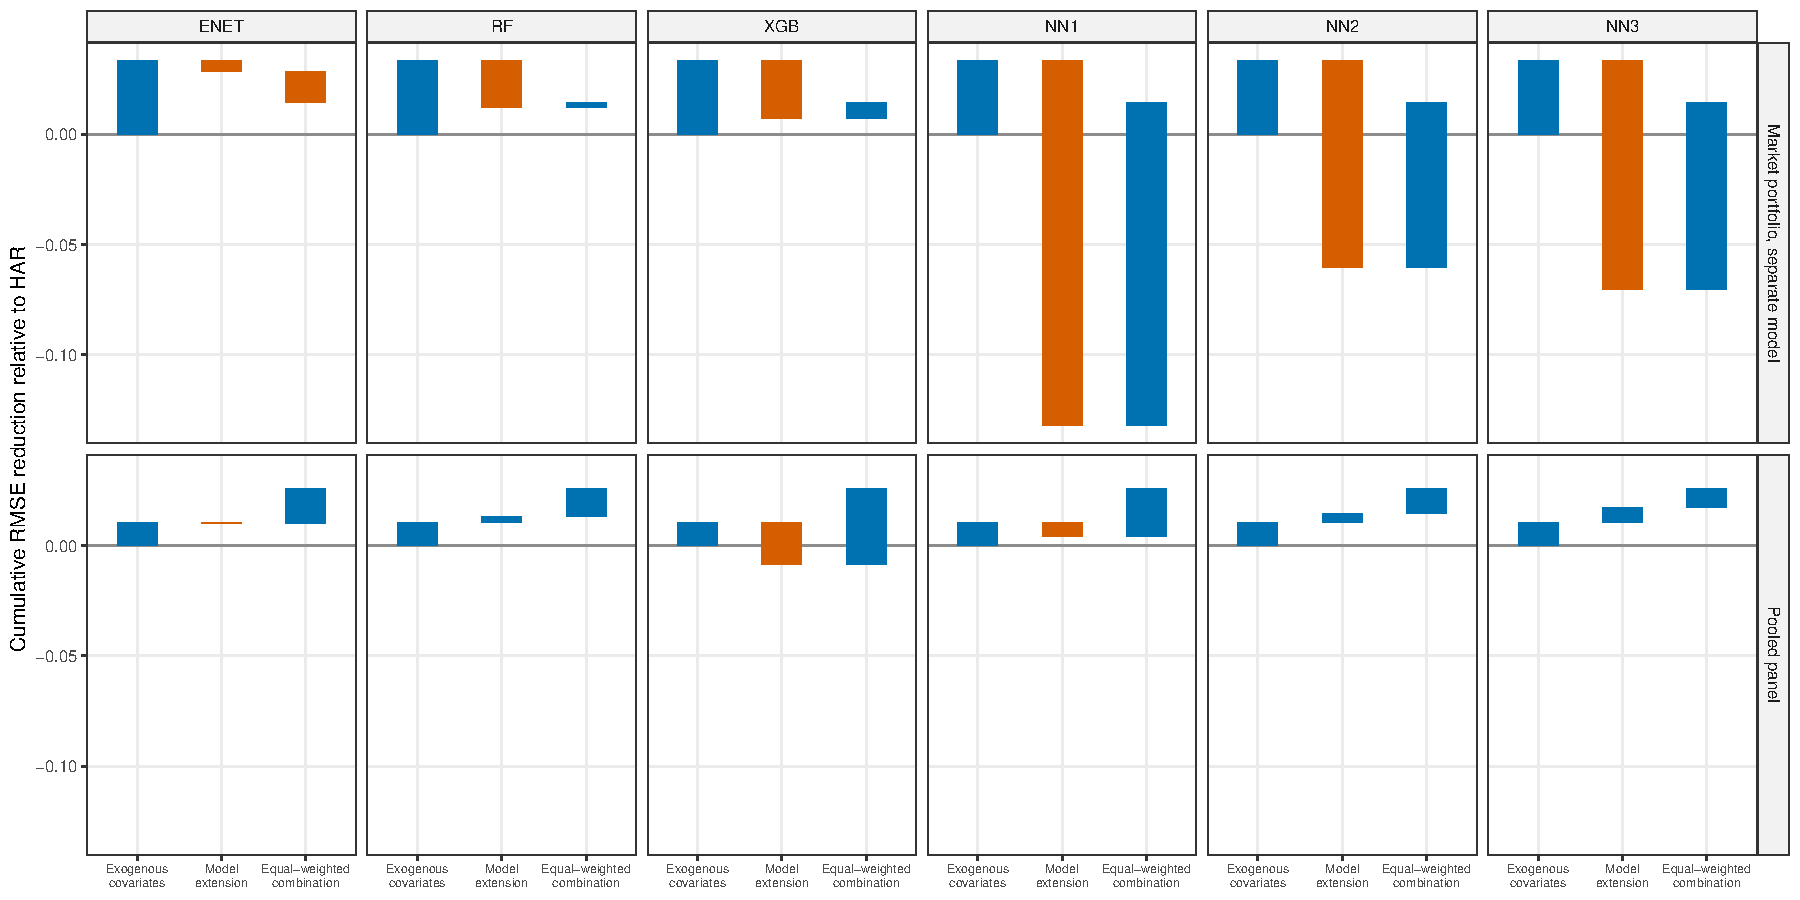
\includegraphics[width=\linewidth,height=0.70\textheight,keepaspectratio]{results_v3/1927/internet_appendix/sequential_waterfall.pdf}
\end{figure}
\begin{figure}[p]
\ContinuedFloat
\centering
\captionsetup{justification=raggedright,labelsep=none,singlelinecheck=false,labelformat=boldlabel}
\caption[]{\footnotesize \textbf{: Sequential changes in out-of-sample RMSE relative to HAR.} Each column considers one extension of HARX. The bars first add exogenous covariates, then the indicated model extension, and finally the equal-weighted forecast combination. Positive changes represent lower RMSE. These arithmetic comparisons do not identify causal contributions. Continued.}
\par\smallskip\textbf{Panel B. Short sample}\par\smallskip
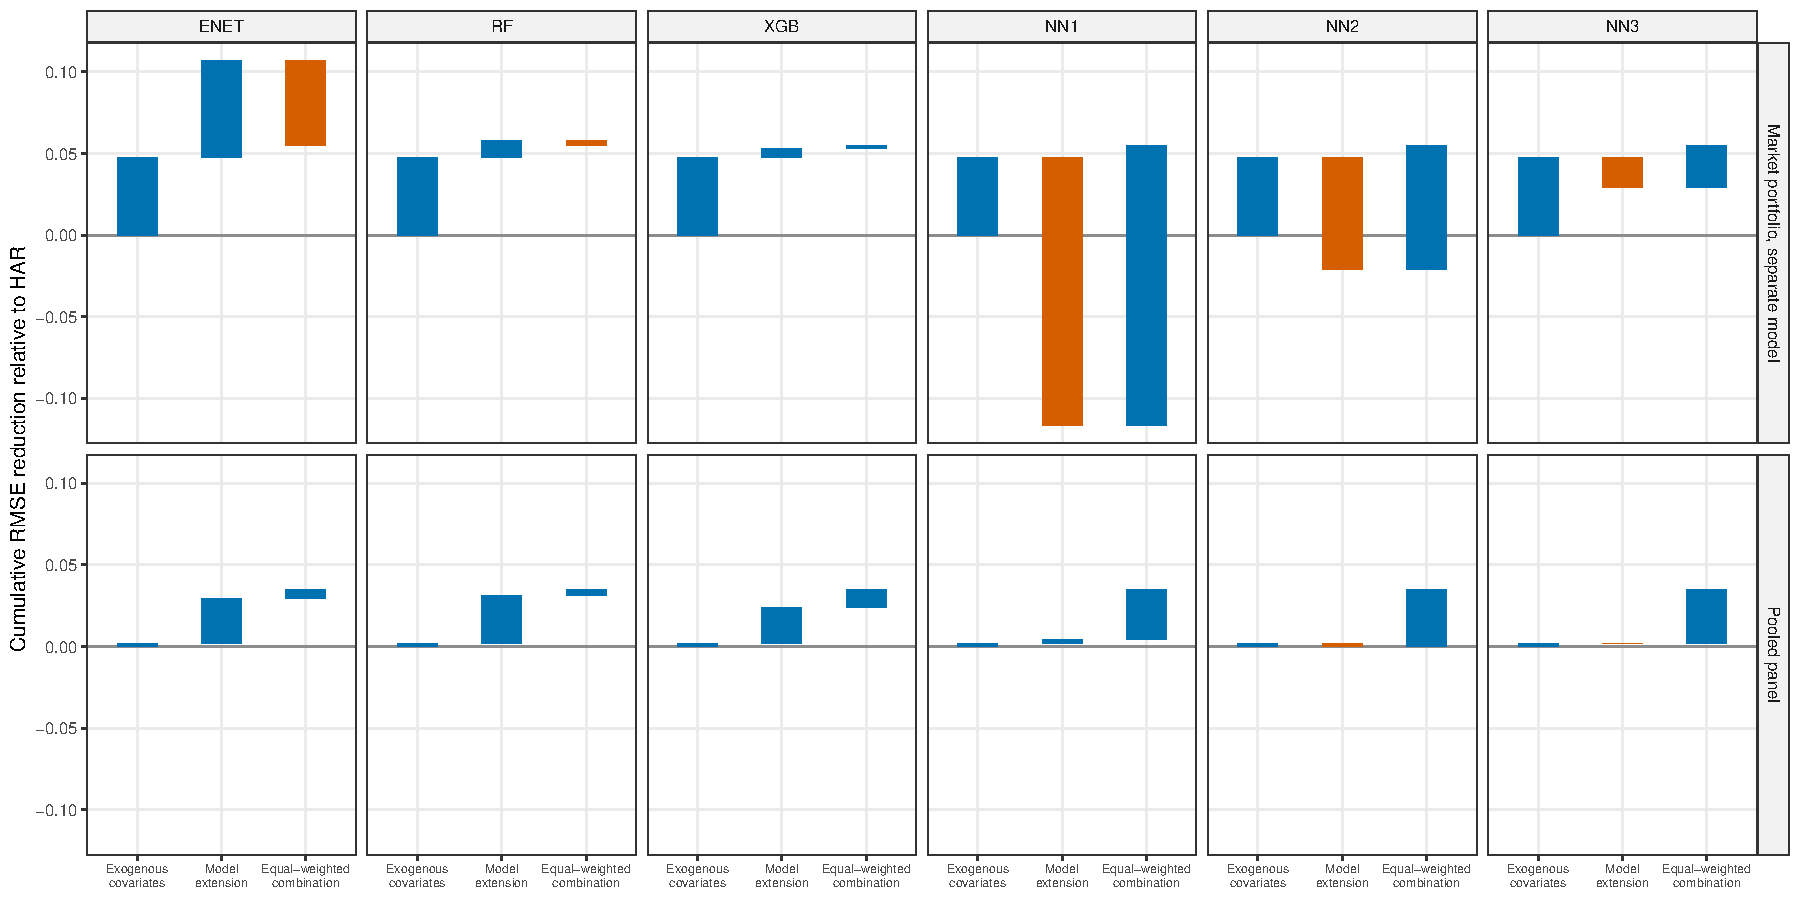
\includegraphics[width=\linewidth,height=0.70\textheight,keepaspectratio]{results_v3/1986/internet_appendix/sequential_waterfall.pdf}
\end{figure}

\begin{figure}[p]
\centering
\captionsetup{justification=raggedright,labelsep=none,singlelinecheck=false,labelformat=boldlabel}
\caption[]{\footnotesize \textbf{: Out-of-sample RMSE gains relative to HAR.} Dots identify the long sample and crosses the short sample. Each comparison uses that sample's HAR. Panel statistics pool squared errors across target-month observations before taking the square root.}
\label{fig:rv-har_relative_gains_market_separate}
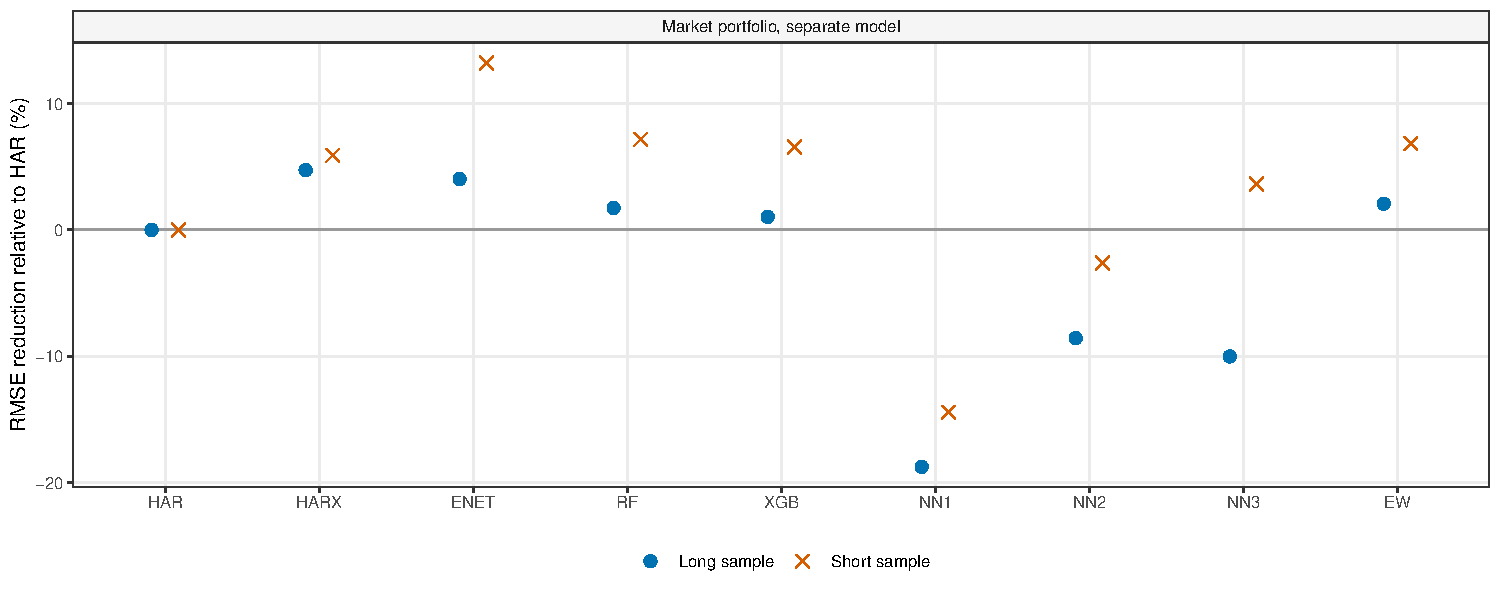
\includegraphics[width=\linewidth,height=0.70\textheight,keepaspectratio]{results_v3/combined/internet_appendix/har_relative_gains_market_separate.pdf}
\end{figure}

\begin{figure}[p]
\centering
\captionsetup{justification=raggedright,labelsep=none,singlelinecheck=false,labelformat=boldlabel}
\caption[]{\footnotesize \textbf{: Trailing 12-month out-of-sample RMSE.} For the pooled-panel result, squared forecast errors are pooled across all available target-month observations in each window before taking the square root. The market-portfolio results evaluate a single monthly series. The figure omits incomplete initial windows.}
\label{fig:rv-rolling_rmse}
\par\smallskip\textbf{Panel A. Long sample}\par\smallskip
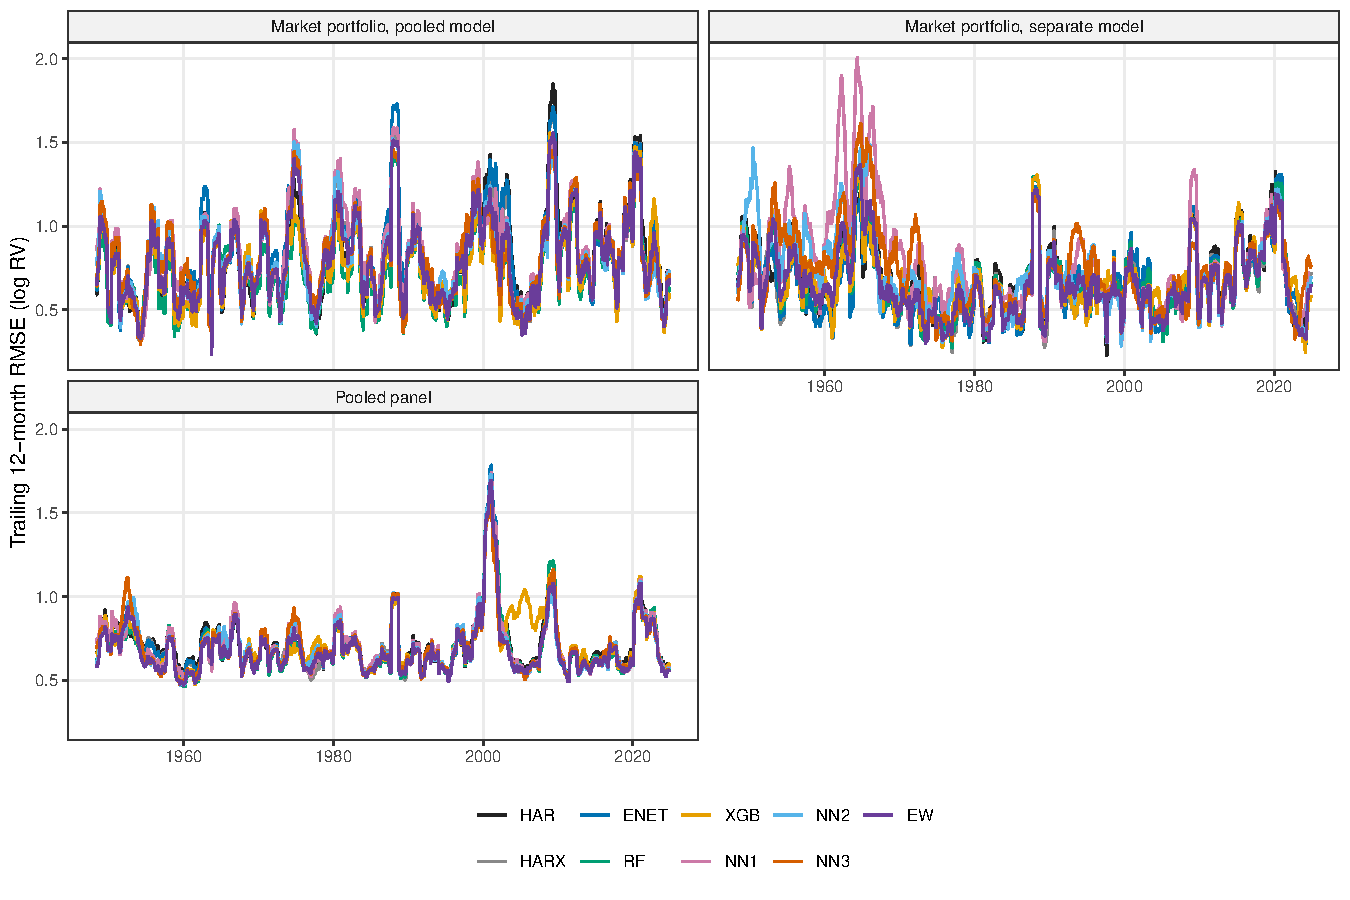
\includegraphics[width=\linewidth,height=0.32\textheight,keepaspectratio]{results_v3/1927/internet_appendix/rolling_rmse.pdf}
\par\smallskip\textbf{Panel B. Short sample}\par\smallskip
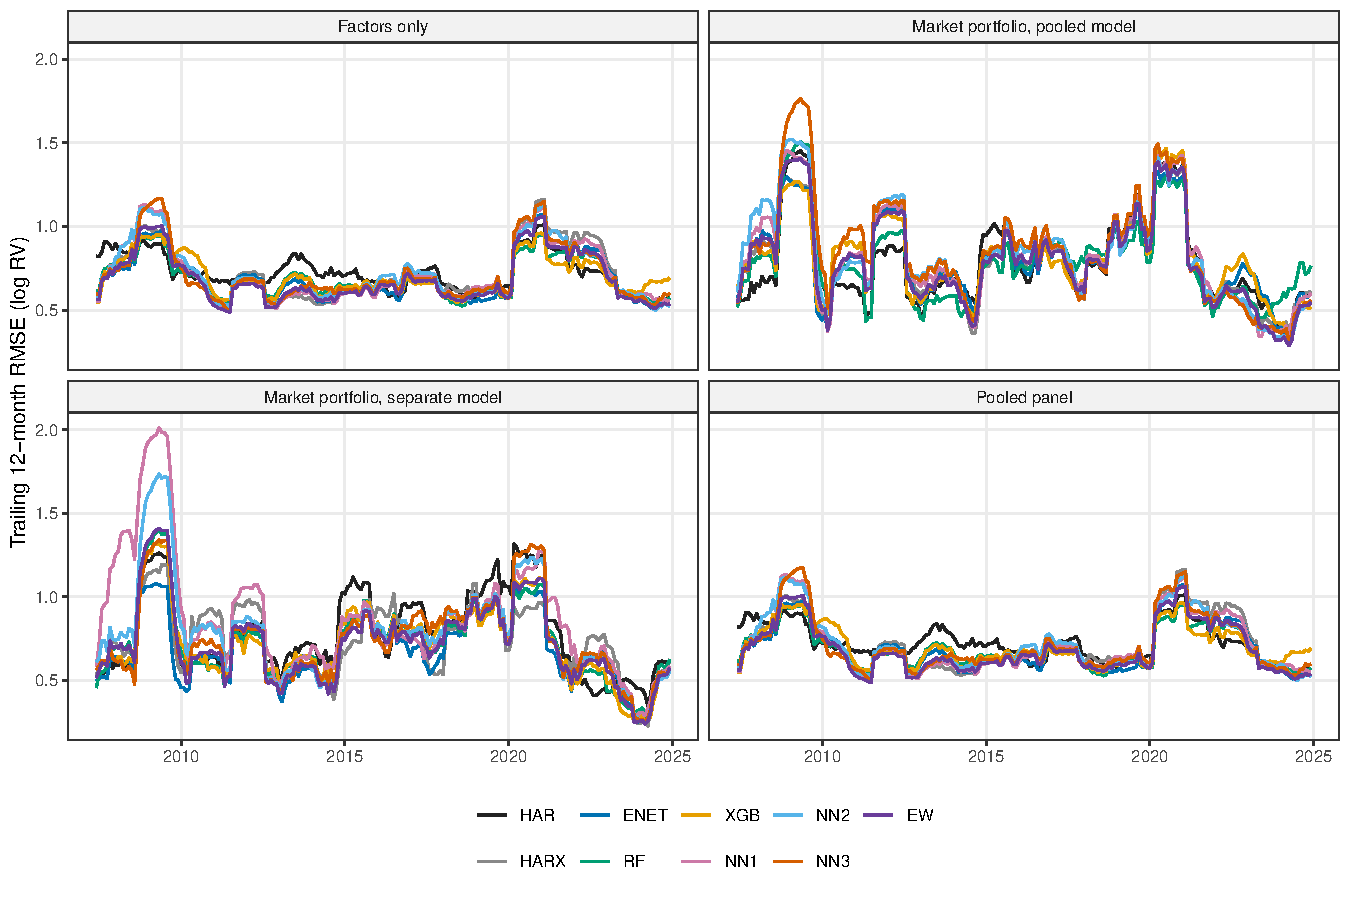
\includegraphics[width=\linewidth,height=0.32\textheight,keepaspectratio]{results_v3/1986/internet_appendix/rolling_rmse.pdf}
\end{figure}

\begin{figure}[p]
\centering
\captionsetup{justification=raggedright,labelsep=none,singlelinecheck=false,labelformat=boldlabel}
\caption[]{\footnotesize \textbf{: Trailing 12-month RMSE of the EW forecast ensemble.} The first panel pools all factor and market errors. The remaining panels pool errors within JKP clusters. Shading shows the interquartile range of factor-level RMSE. Both sample histories are shown on the same date axis.}
\label{fig:rv-cluster_rolling_rmse}
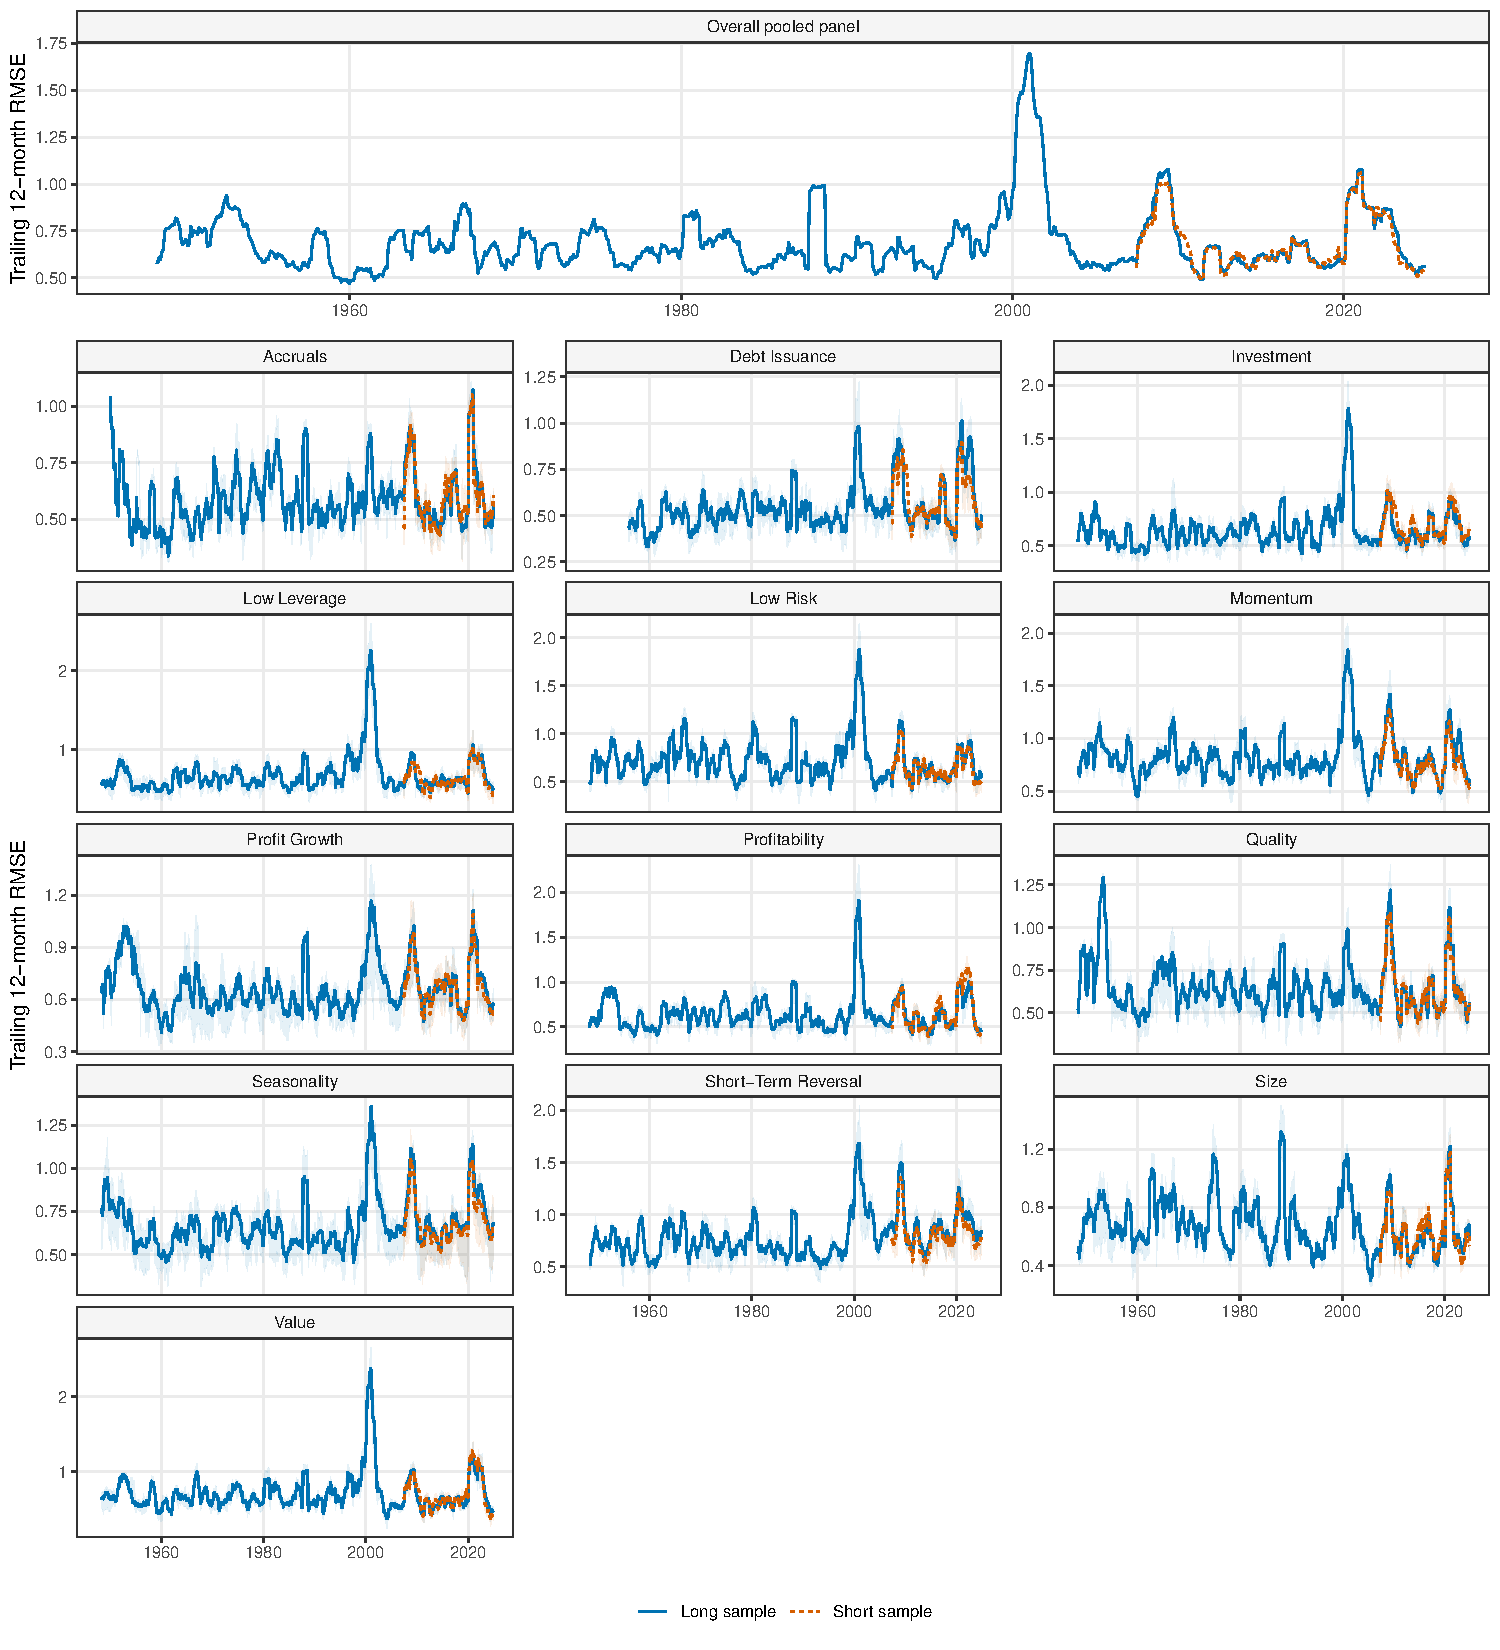
\includegraphics[width=\linewidth,height=0.70\textheight,keepaspectratio]{results_v3/combined/internet_appendix/cluster_rolling_rmse.pdf}
\end{figure}

\begin{figure}[p]
\centering
\captionsetup{justification=raggedright,labelsep=none,singlelinecheck=false,labelformat=boldlabel}
\caption[]{\footnotesize \textbf{: Validation RMSE and subsequent out-of-sample RMSE after each annual model selection.} Validation windows contain 90 months and subsequent forecast blocks normally contain 12 months. Neural-network validation uses one fitted network, while out-of-sample forecasts average ten independent refits. Differences may therefore reflect refitting, sample length, and changes in volatility conditions.}
\label{fig:rv-validation_test}
\par\smallskip\textbf{Panel A. Long sample}\par\smallskip
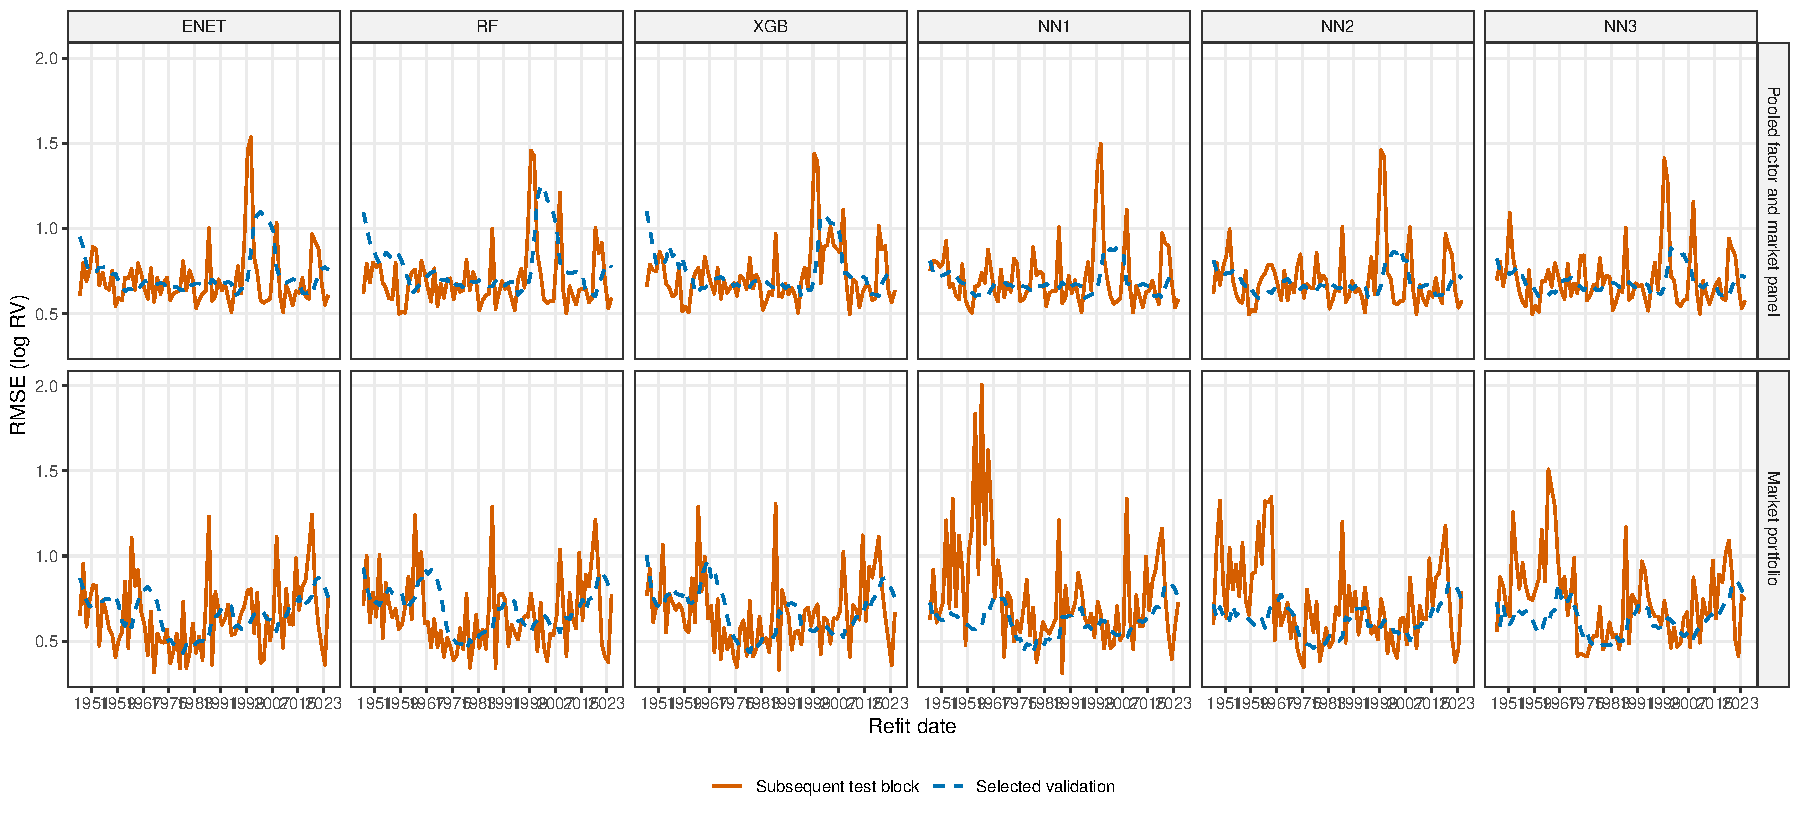
\includegraphics[width=\linewidth,height=0.70\textheight,keepaspectratio]{results_v3/1927/internet_appendix/validation_test.pdf}
\end{figure}
\begin{figure}[p]
\ContinuedFloat
\centering
\captionsetup{justification=raggedright,labelsep=none,singlelinecheck=false,labelformat=boldlabel}
\caption[]{\footnotesize \textbf{: Validation RMSE and subsequent out-of-sample RMSE after each annual model selection.} Validation windows contain 90 months and subsequent forecast blocks normally contain 12 months. Neural-network validation uses one fitted network, while out-of-sample forecasts average ten independent refits. Differences may therefore reflect refitting, sample length, and changes in volatility conditions. Continued.}
\par\smallskip\textbf{Panel B. Short sample}\par\smallskip
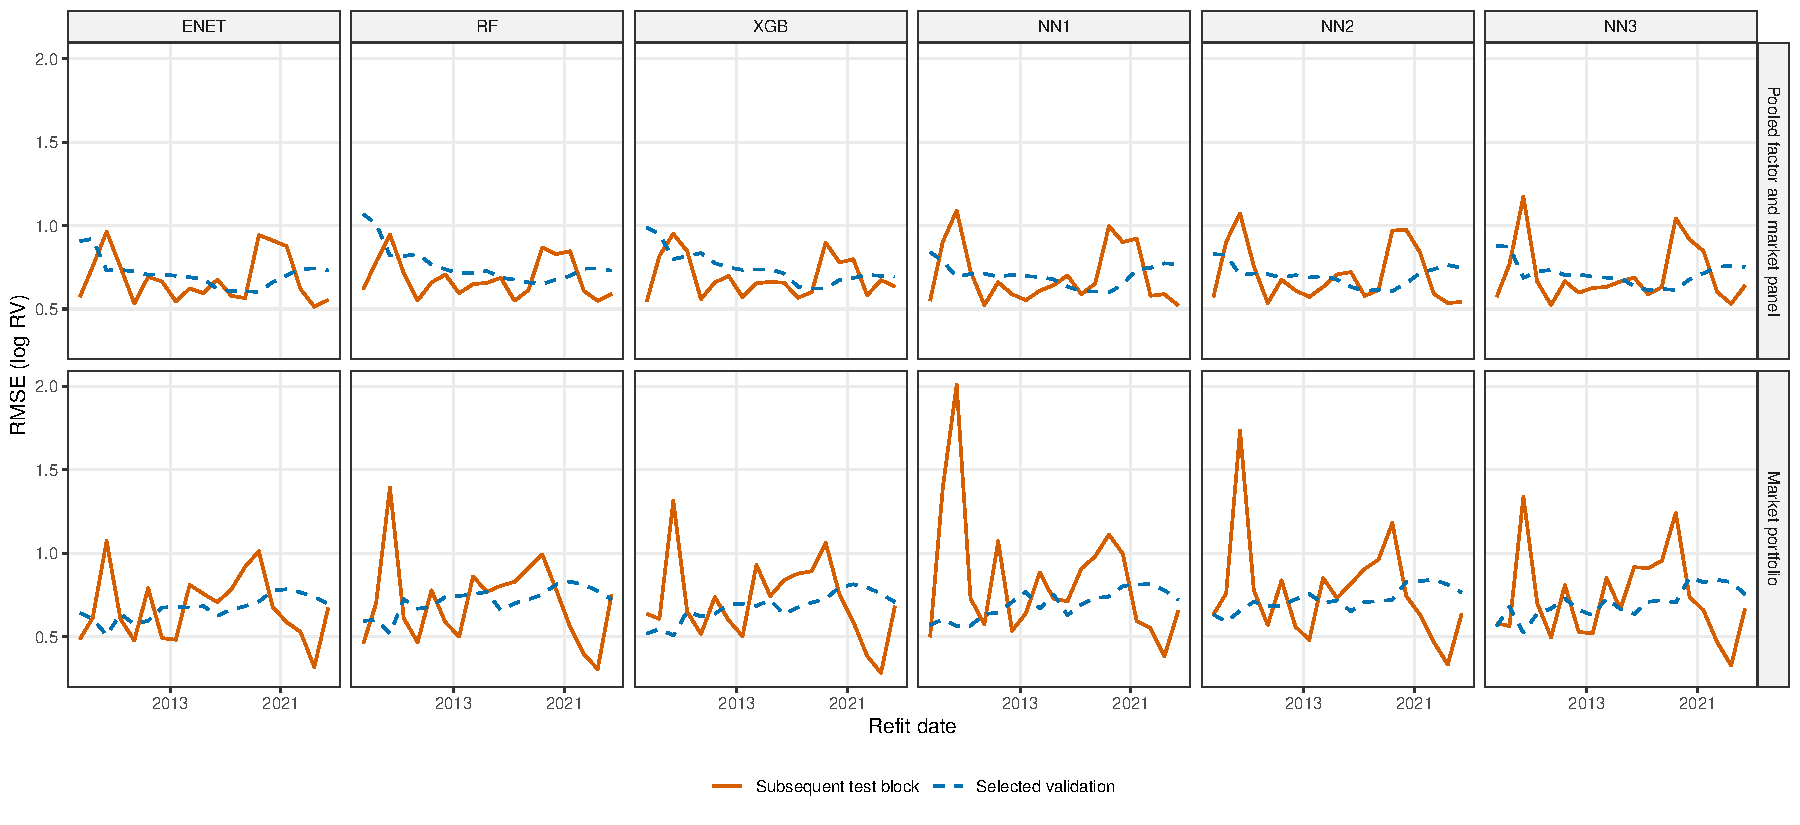
\includegraphics[width=\linewidth,height=0.70\textheight,keepaspectratio]{results_v3/1986/internet_appendix/validation_test.pdf}
\end{figure}

\begin{figure}[p]
\centering
\captionsetup{justification=raggedright,labelsep=none,singlelinecheck=false,labelformat=boldlabel}
\caption[]{\footnotesize \textbf{: Selected hyperparameters at each annual refit.} Each panel identifies the model and parameter. Lines compare pooled-panel estimation with separate market-portfolio estimation. The boosting iteration count is selected by early stopping.}
\label{fig:rv-hyperparameters_all}
\par\smallskip\textbf{Panel A. Long sample}\par\smallskip
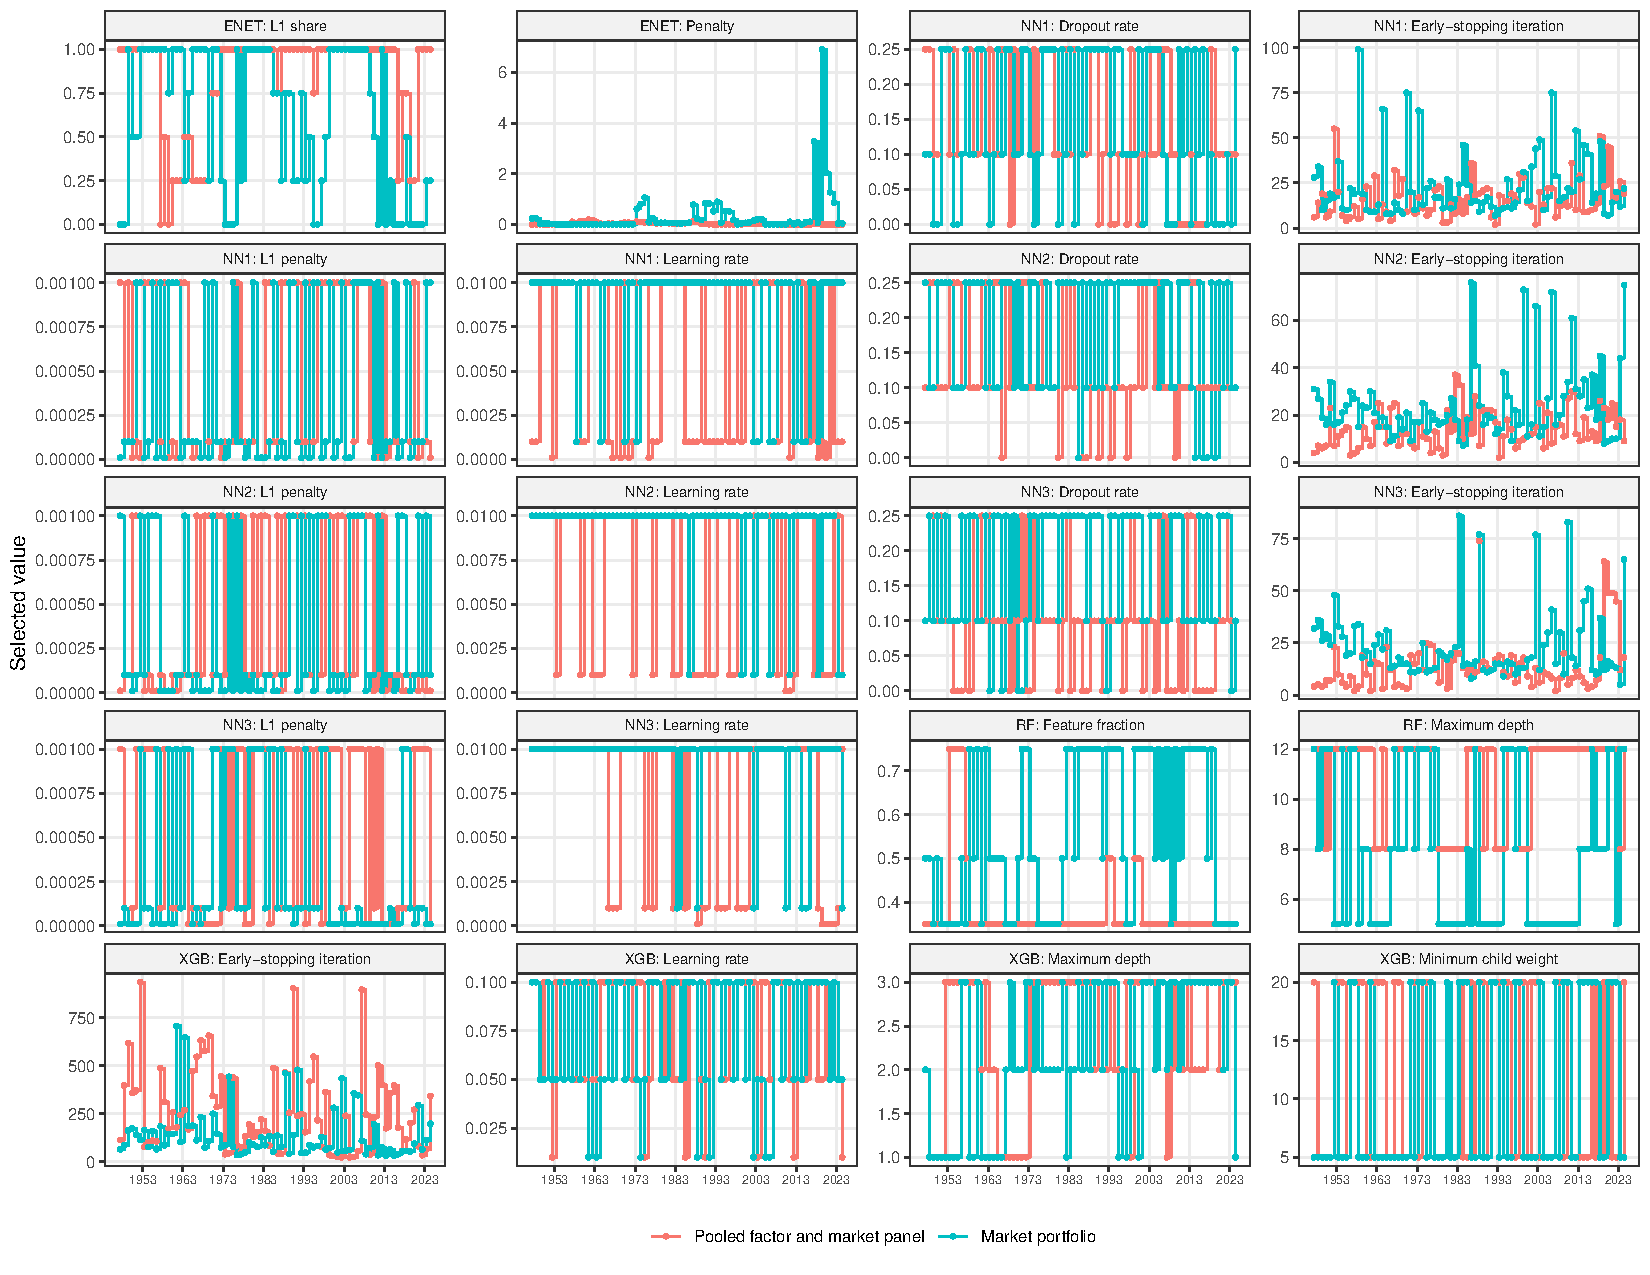
\includegraphics[width=\linewidth,height=0.70\textheight,keepaspectratio]{results_v3/1927/internet_appendix/hyperparameters_all.pdf}
\end{figure}
\begin{figure}[p]
\ContinuedFloat
\centering
\captionsetup{justification=raggedright,labelsep=none,singlelinecheck=false,labelformat=boldlabel}
\caption[]{\footnotesize \textbf{: Selected hyperparameters at each annual refit.} Each panel identifies the model and parameter. Lines compare pooled-panel estimation with separate market-portfolio estimation. The boosting iteration count is selected by early stopping. Continued.}
\par\smallskip\textbf{Panel B. Short sample}\par\smallskip
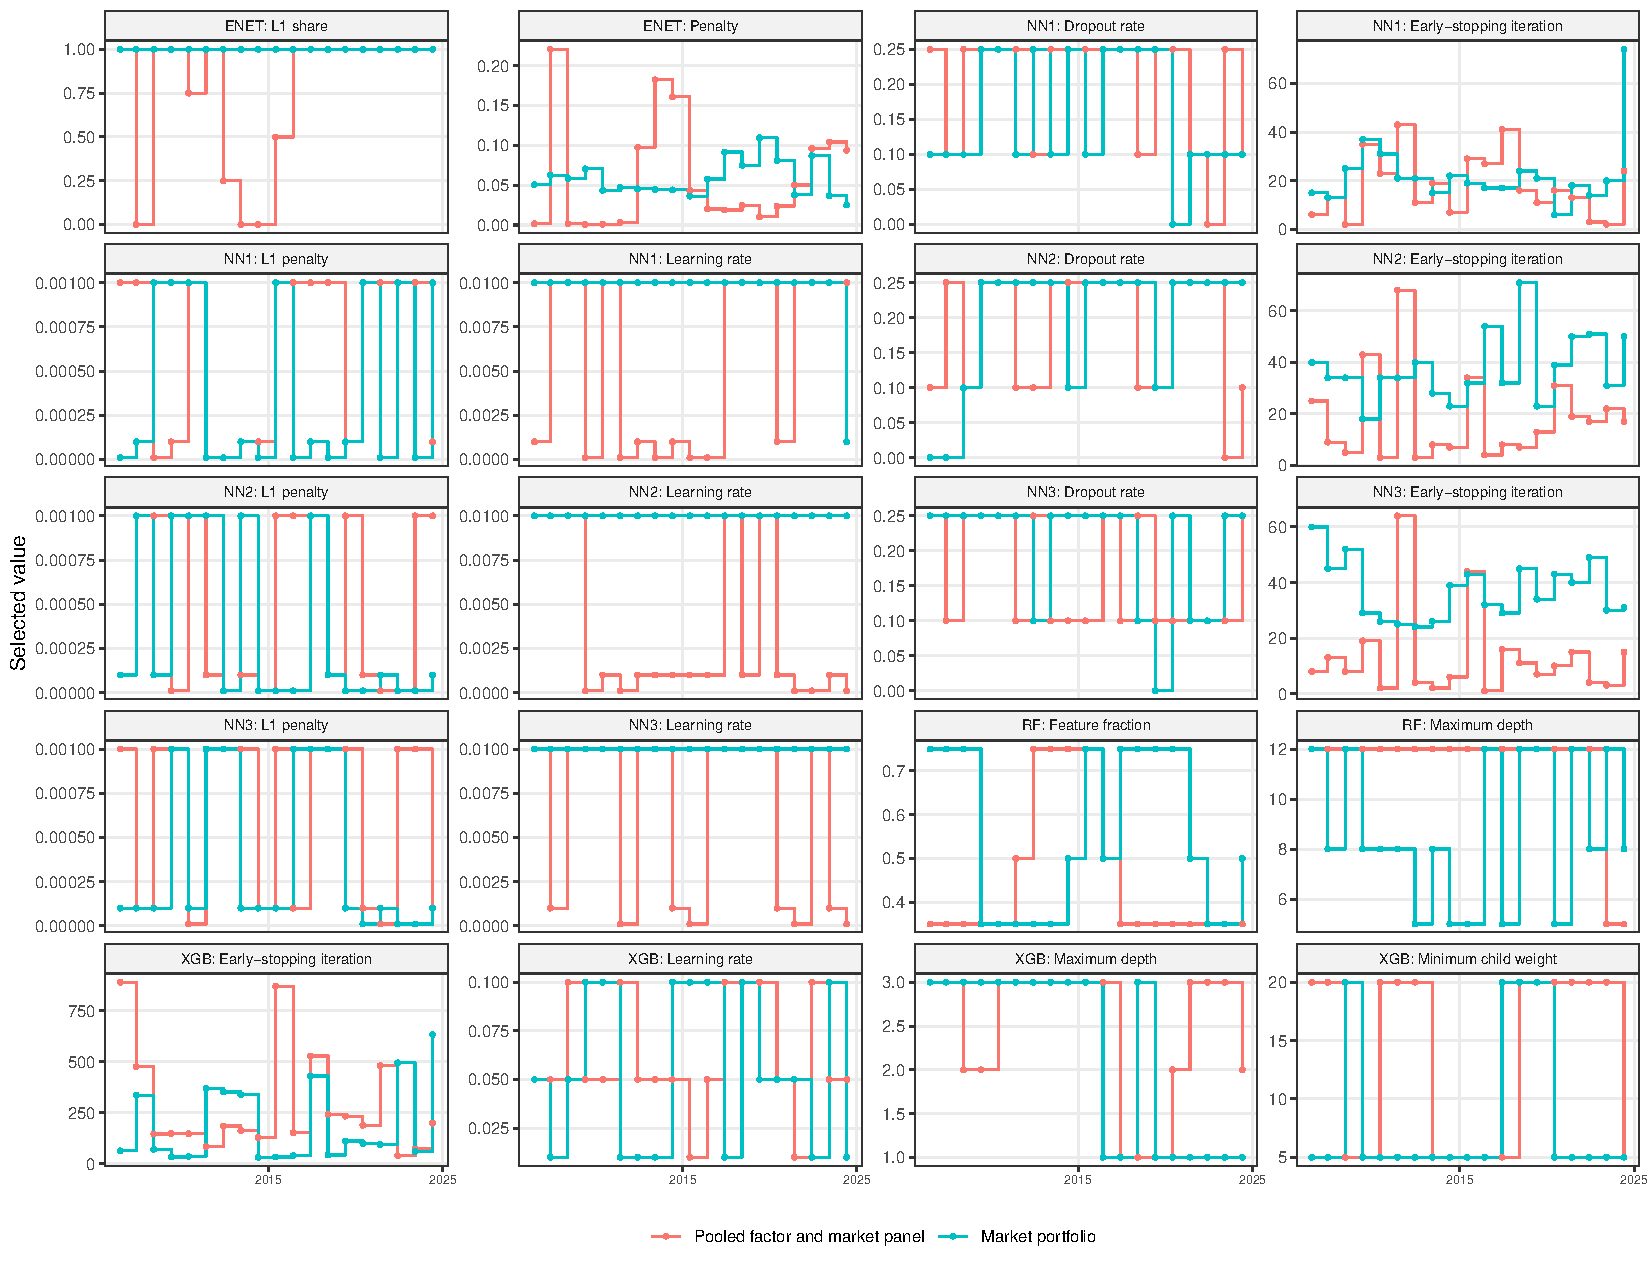
\includegraphics[width=\linewidth,height=0.70\textheight,keepaspectratio]{results_v3/1986/internet_appendix/hyperparameters_all.pdf}
\end{figure}

\begin{figure}[p]
\centering
\captionsetup{justification=raggedright,labelsep=none,singlelinecheck=false,labelformat=boldlabel}
\caption[]{\footnotesize \textbf{: Predictor-theme signed loading shares at the final model refit.} Panel A reports the long sample and Panel B the short sample. Columns distinguish pooled and separate market estimation. Linear surrogate coefficients are normalized by the sum of absolute non-intercept coefficients before aggregation by theme. Blank cells indicate absent loadings. These descriptive associations are not causal importance measures.}
\label{fig:rv-final_theme_net_share}
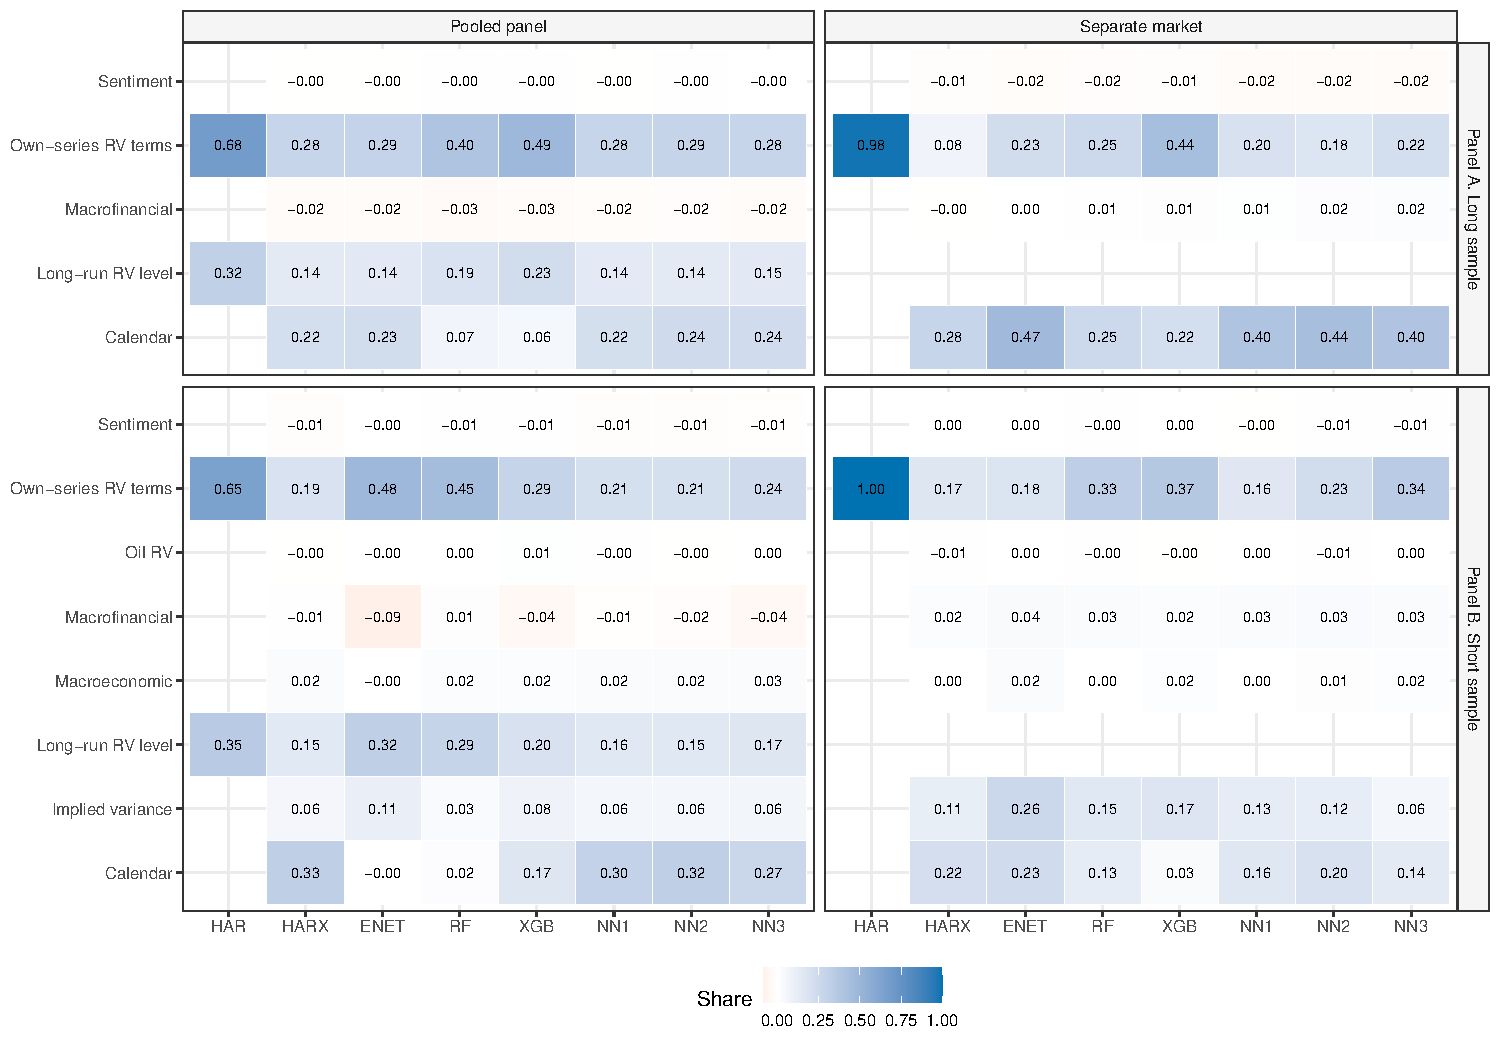
\includegraphics[width=\linewidth,height=0.70\textheight,keepaspectratio]{results_v3/combined/internet_appendix/final_theme_net_share.pdf}
\end{figure}

\begin{figure}[p]
\centering
\captionsetup{justification=raggedright,labelsep=none,singlelinecheck=false,labelformat=boldlabel}
\caption[]{\footnotesize \textbf{: Predictor-theme loading shares over time for the Pooled factor and market panel estimation.} The figure reports descriptive loadings from linear surrogate models. Columns report HAR, HARX, elastic net, random forest, XGBoost, and the three neural-network architectures. The intercept is excluded. Each coefficient is divided by the sum of absolute non-intercept coefficients. Gross shares sum absolute loadings within themes. Net shares retain coefficient signs. Own-series terms refer to each factor's realized measures. The equal-weighted forecast has no fitted surrogate model.}
\label{fig:rv-theme_history_panel}
\par\smallskip\textbf{Panel A. Long sample}\par\smallskip
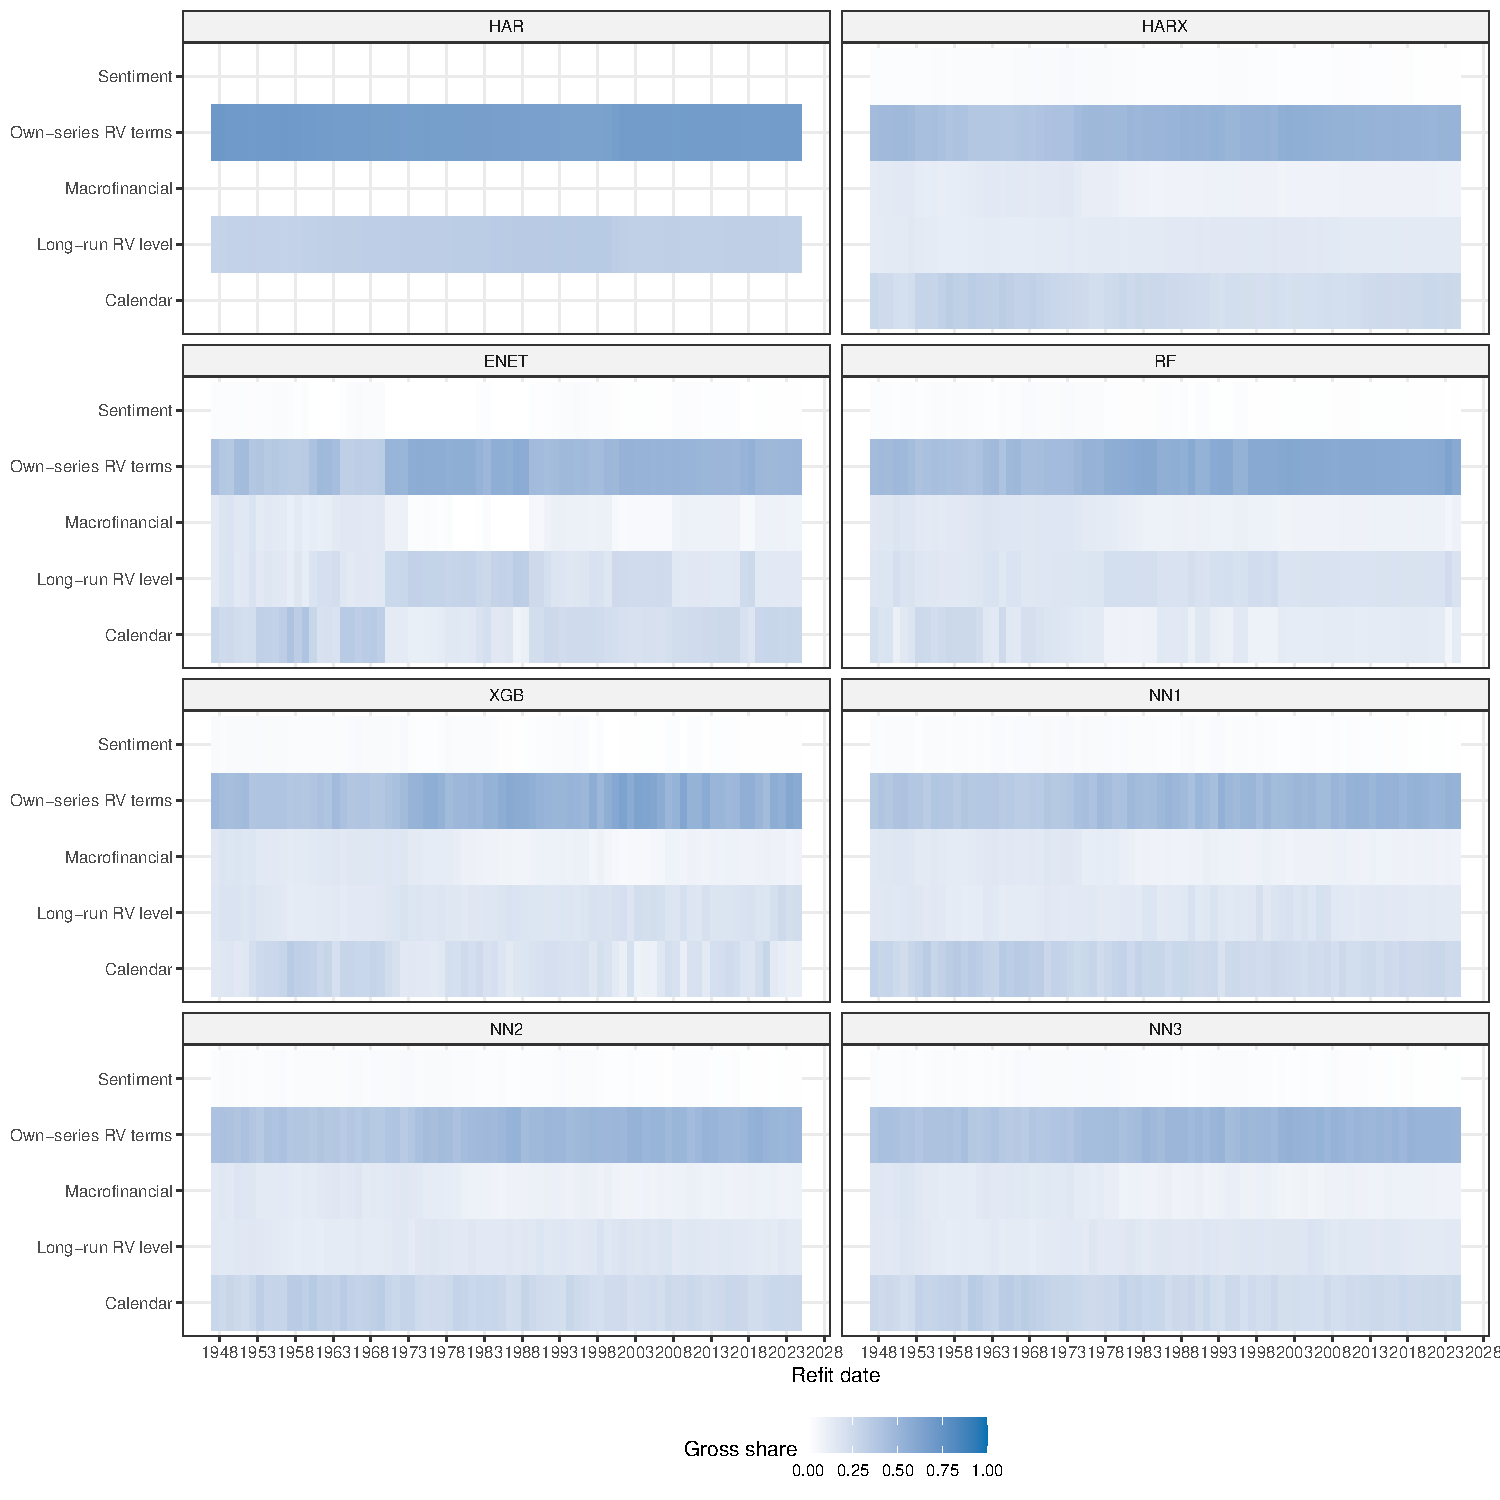
\includegraphics[width=\linewidth,height=0.70\textheight,keepaspectratio]{results_v3/1927/internet_appendix/theme_history_panel.pdf}
\end{figure}
\begin{figure}[p]
\ContinuedFloat
\centering
\captionsetup{justification=raggedright,labelsep=none,singlelinecheck=false,labelformat=boldlabel}
\caption[]{\footnotesize \textbf{: Predictor-theme loading shares over time for the Pooled factor and market panel estimation.} The figure reports descriptive loadings from linear surrogate models. Columns report HAR, HARX, elastic net, random forest, XGBoost, and the three neural-network architectures. The intercept is excluded. Each coefficient is divided by the sum of absolute non-intercept coefficients. Gross shares sum absolute loadings within themes. Net shares retain coefficient signs. Own-series terms refer to each factor's realized measures. The equal-weighted forecast has no fitted surrogate model. Continued.}
\par\smallskip\textbf{Panel B. Short sample}\par\smallskip
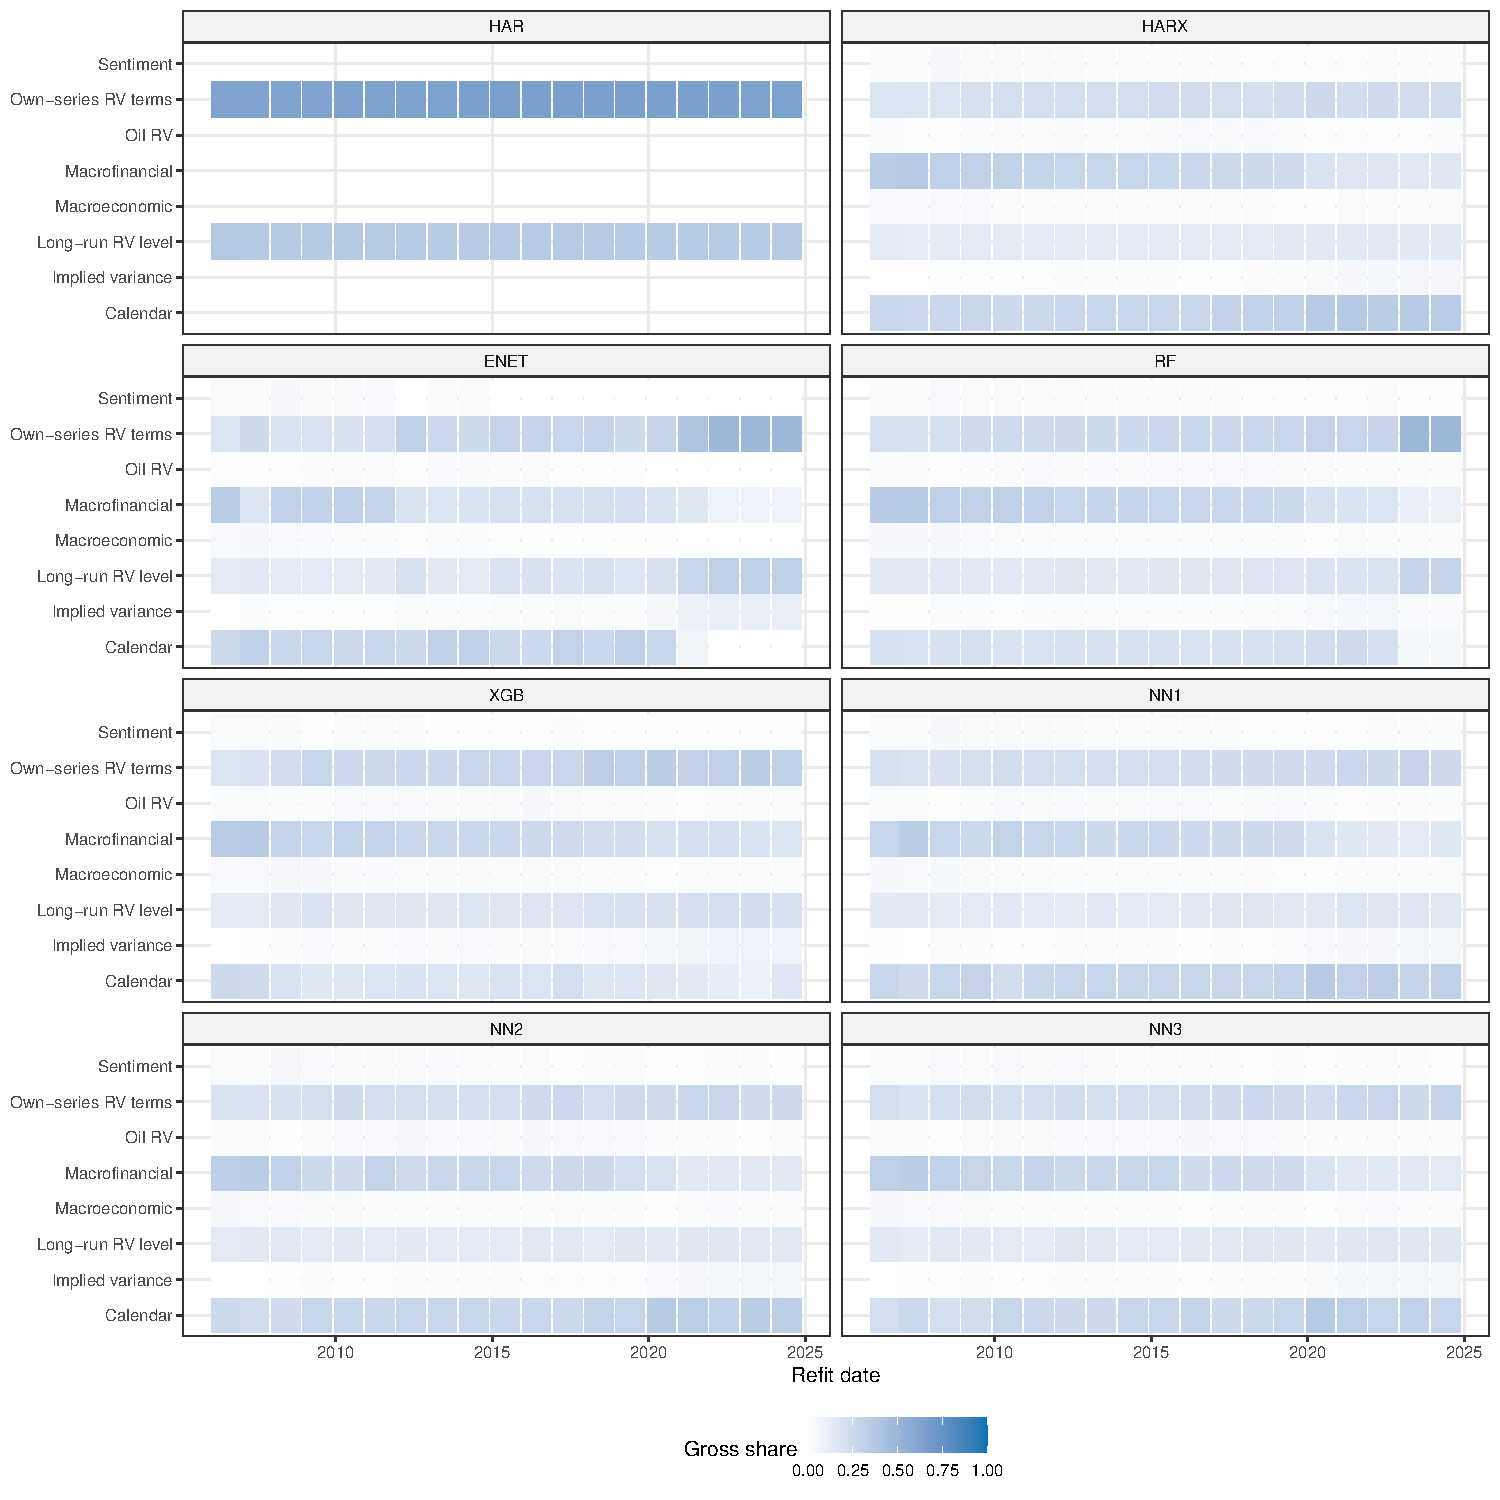
\includegraphics[width=\linewidth,height=0.70\textheight,keepaspectratio]{results_v3/1986/internet_appendix/theme_history_panel.pdf}
\end{figure}

\begin{figure}[p]
\centering
\captionsetup{justification=raggedright,labelsep=none,singlelinecheck=false,labelformat=boldlabel}
\caption[]{\footnotesize \textbf{: Predictor-theme loading shares over time for the Market portfolio estimation.} The figure reports descriptive loadings from linear surrogate models. Columns report HAR, HARX, elastic net, random forest, XGBoost, and the three neural-network architectures. The intercept is excluded. Each coefficient is divided by the sum of absolute non-intercept coefficients. Gross shares sum absolute loadings within themes. Net shares retain coefficient signs. Own-series terms refer to each factor's realized measures. The equal-weighted forecast has no fitted surrogate model.}
\label{fig:rv-theme_history_spx}
\par\smallskip\textbf{Panel A. Long sample}\par\smallskip
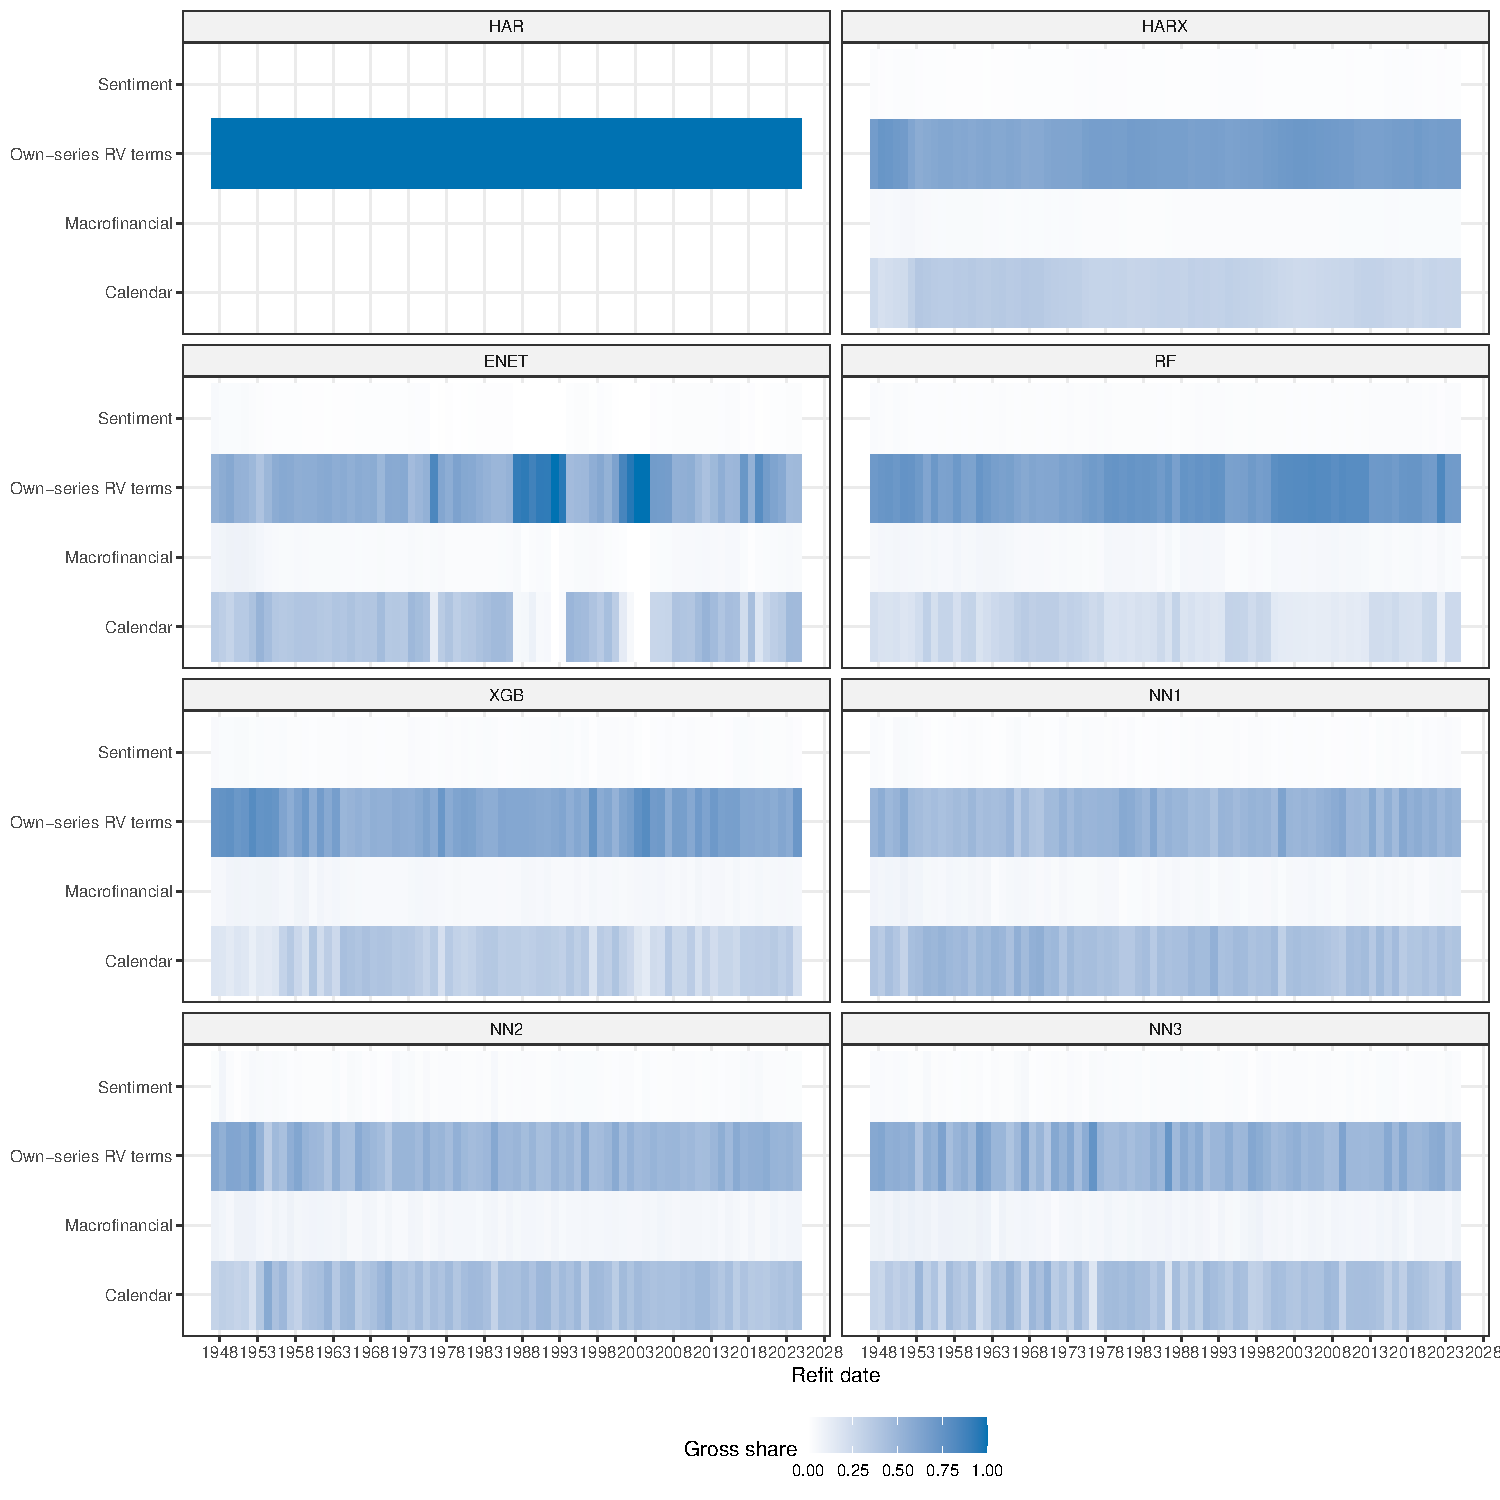
\includegraphics[width=\linewidth,height=0.70\textheight,keepaspectratio]{results_v3/1927/internet_appendix/theme_history_spx.pdf}
\end{figure}
\begin{figure}[p]
\ContinuedFloat
\centering
\captionsetup{justification=raggedright,labelsep=none,singlelinecheck=false,labelformat=boldlabel}
\caption[]{\footnotesize \textbf{: Predictor-theme loading shares over time for the Market portfolio estimation.} The figure reports descriptive loadings from linear surrogate models. Columns report HAR, HARX, elastic net, random forest, XGBoost, and the three neural-network architectures. The intercept is excluded. Each coefficient is divided by the sum of absolute non-intercept coefficients. Gross shares sum absolute loadings within themes. Net shares retain coefficient signs. Own-series terms refer to each factor's realized measures. The equal-weighted forecast has no fitted surrogate model. Continued.}
\par\smallskip\textbf{Panel B. Short sample}\par\smallskip
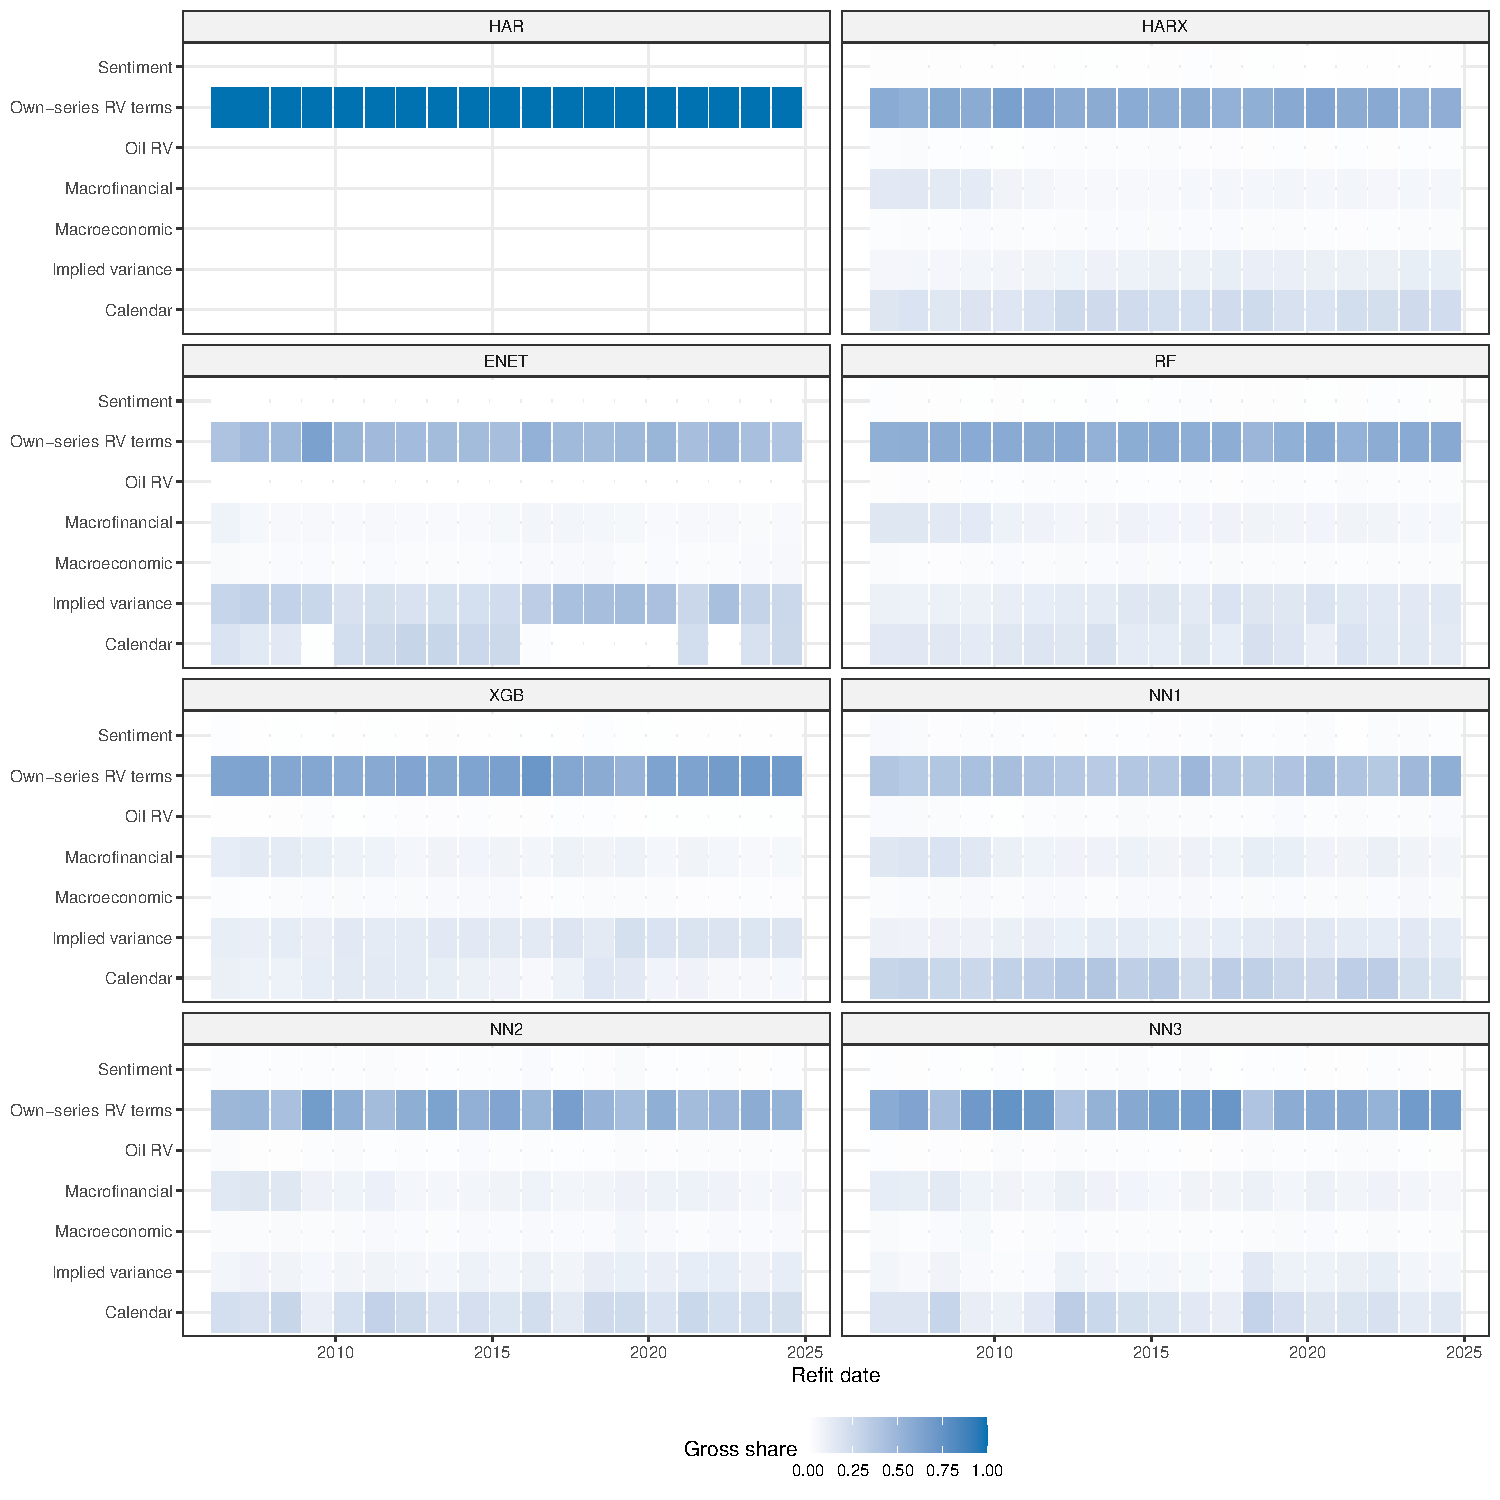
\includegraphics[width=\linewidth,height=0.70\textheight,keepaspectratio]{results_v3/1986/internet_appendix/theme_history_spx.pdf}
\end{figure}

\begin{figure}[p]
\centering
\captionsetup{justification=raggedright,labelsep=none,singlelinecheck=false,labelformat=boldlabel}
\caption[]{\footnotesize \textbf{: Gross and net Sharpe ratios for the market portfolio using separate forecasts.} Panel A reports the long sample and Panel B the short sample. Pale bars are gross and solid bars are net of modeled factor-exposure costs. EW denotes the forecast ensemble. Each construction retains its stated exposure cap. }
\label{fig:rv-portfolio_wealth_market_separate}
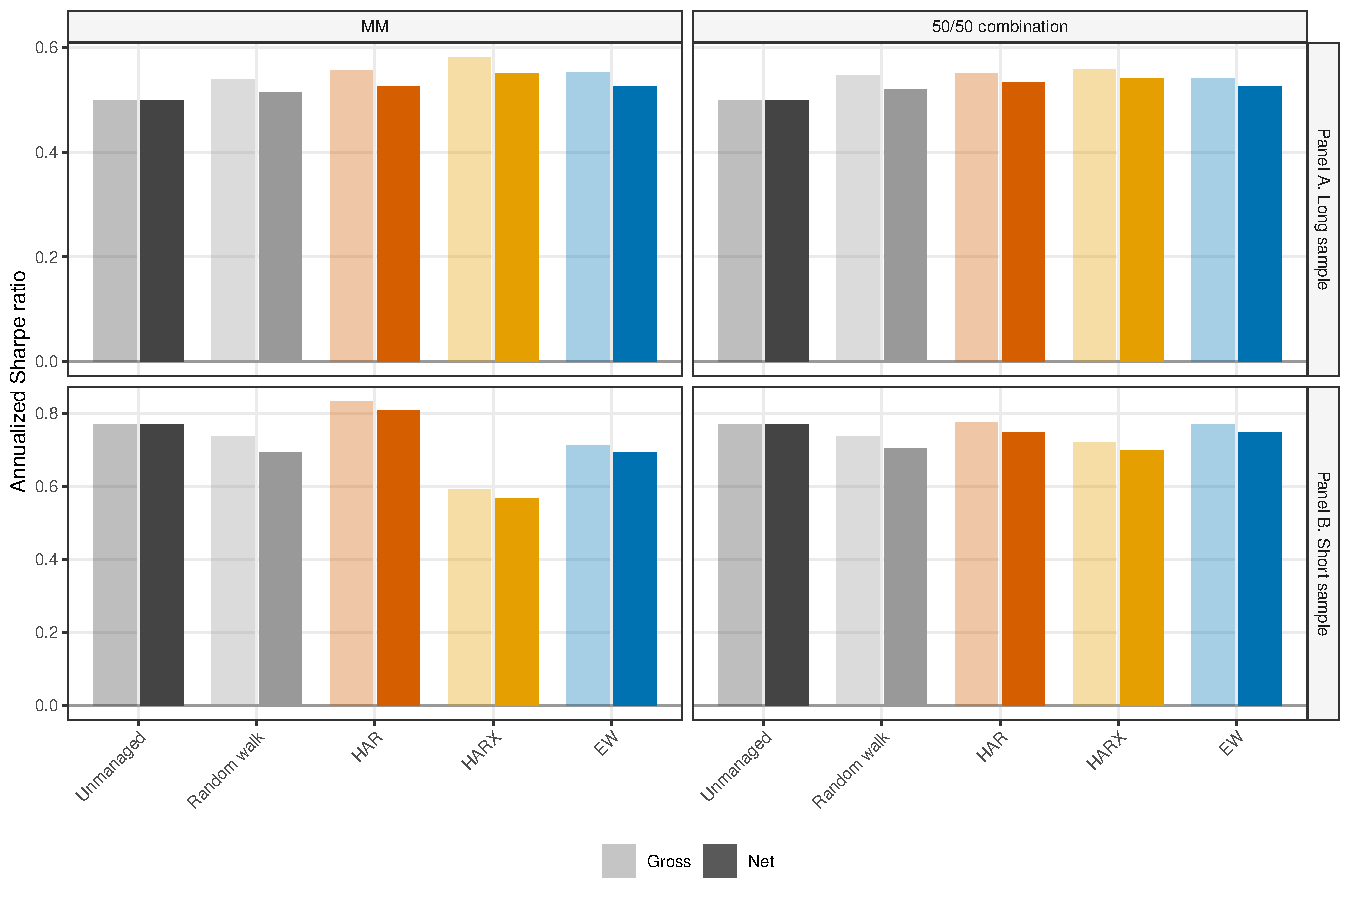
\includegraphics[width=\linewidth,height=0.70\textheight,keepaspectratio]{results_v3/combined/internet_appendix/portfolio_wealth_market_separate.pdf}
\end{figure}

\begin{landscape}
\begingroup\scriptsize
\captionsetup{justification=raggedright,labelsep=none,singlelinecheck=false,labelformat=boldlabel}
\setlength{\tabcolsep}{2.5pt}
\begin{longtable}{>{\raggedright\arraybackslash}p{2.6cm}rrrrrrrrrrr}
\caption[Net Sharpe ratios of volatility-managed factor portfolios by Jensen, Kelly, and Pedersen factor cluster.]{\footnotesize \textbf{: Long sample. Net Sharpe ratios of volatility-managed factor portfolios by Jensen, Kelly, and Pedersen factor cluster.} The first row of each panel reports the Sharpe ratio of an equal-weighted portfolio of the factors in that cluster. The remaining rows report individual factor strategies. All managed strategies cap exposure at 1.5 and deduct 10 basis points per unit change in factor exposure. Light blue cells identify strategies that outperform the strongest result between the unmanaged and random-walk benchmarks. Bold cells identify the highest Sharpe ratio in each row.}\label{tab:rv-portfolio_factor_sharpe}\\
\hline
Factor & Unmanaged & Random walk & HAR & HARX & ENET & RF & XGB & NN1 & NN2 & NN3 & EW \\
\hline\endfirsthead
\hline
Factor & Unmanaged & Random walk & HAR & HARX & ENET & RF & XGB & NN1 & NN2 & NN3 & EW \\
\hline\endhead
\hline\endfoot
\multicolumn{12}{@{}l}{\textit{Panel A. Accruals}} \\
\hline
Factor & Unmanaged & Random walk & HAR & HARX & ENET & RF & XGB & NN1 & NN2 & NN3 & EW \\
\hline
\textbf{Cluster aggregate} & \textbf{0.633} & 0.533 & 0.574 & 0.556 & 0.575 & 0.592 & 0.610 & 0.571 & 0.589 & 0.574 & 0.586 \\
cowc\_gr1a & 0.810 & 0.758 & 0.770 & 0.755 & 0.775 & 0.810 & \textbf{\cellcolor{blue!10}0.819} & 0.777 & 0.792 & 0.801 & 0.795 \\
oaccruals\_at & 0.684 & 0.673 & \cellcolor{blue!10}0.731 & \cellcolor{blue!10}0.699 & \cellcolor{blue!10}0.730 & \cellcolor{blue!10}0.730 & \textbf{\cellcolor{blue!10}0.757} & \cellcolor{blue!10}0.716 & \cellcolor{blue!10}0.736 & \cellcolor{blue!10}0.709 & \cellcolor{blue!10}0.731 \\
oaccruals\_ni & \textbf{0.764} & 0.622 & 0.718 & 0.692 & 0.709 & 0.721 & 0.702 & 0.704 & 0.721 & 0.685 & 0.710 \\
seas\_16\_20na & 0.062 & 0.111 & 0.109 & \cellcolor{blue!10}0.121 & \cellcolor{blue!10}0.113 & \cellcolor{blue!10}0.120 & \textbf{\cellcolor{blue!10}0.127} & 0.104 & \cellcolor{blue!10}0.111 & \cellcolor{blue!10}0.124 & \cellcolor{blue!10}0.119 \\
taccruals\_at & \textbf{0.251} & 0.169 & 0.165 & 0.148 & 0.171 & 0.194 & 0.231 & 0.160 & 0.176 & 0.177 & 0.183 \\
taccruals\_ni & \textbf{0.214} & 0.114 & 0.138 & 0.125 & 0.128 & 0.154 & 0.160 & 0.146 & 0.152 & 0.141 & 0.148 \\
\hline
\multicolumn{12}{@{}l}{\textit{Panel B. Debt Issuance}} \\
\hline
Factor & Unmanaged & Random walk & HAR & HARX & ENET & RF & XGB & NN1 & NN2 & NN3 & EW \\
\hline
\textbf{Cluster aggregate} & 1.022 & 0.900 & 0.979 & 0.948 & 0.975 & \textbf{\cellcolor{blue!10}1.023} & 0.977 & 0.971 & 1.006 & 0.988 & 0.995 \\
capex\_abn & 0.629 & 0.538 & 0.619 & 0.611 & 0.620 & \textbf{\cellcolor{blue!10}0.642} & 0.625 & 0.620 & 0.619 & 0.603 & \cellcolor{blue!10}0.629 \\
debt\_gr3 & 0.553 & 0.564 & \cellcolor{blue!10}0.574 & 0.550 & \cellcolor{blue!10}0.565 & \textbf{\cellcolor{blue!10}0.598} & 0.517 & 0.545 & 0.560 & 0.546 & 0.560 \\
fnl\_gr1a & \textbf{0.856} & 0.775 & 0.817 & 0.804 & 0.827 & 0.849 & 0.749 & 0.829 & 0.848 & 0.846 & 0.830 \\
ncol\_gr1a & \textbf{0.080} & -0.123 & -0.070 & -0.073 & -0.062 & -0.019 & -0.063 & -0.047 & 0.001 & -0.034 & -0.042 \\
nfna\_gr1a & \textbf{0.951} & 0.829 & 0.867 & 0.869 & 0.894 & 0.909 & 0.853 & 0.896 & 0.915 & 0.907 & 0.896 \\
ni\_ar1 & 0.091 & -0.033 & -0.016 & -0.060 & -0.026 & 0.082 & \textbf{\cellcolor{blue!10}0.094} & -0.072 & 0.003 & 0.022 & 0.010 \\
noa\_at & 0.993 & 1.180 & \textbf{\cellcolor{blue!10}1.238} & \cellcolor{blue!10}1.217 & \cellcolor{blue!10}1.234 & \cellcolor{blue!10}1.195 & \cellcolor{blue!10}1.216 & \cellcolor{blue!10}1.223 & \cellcolor{blue!10}1.236 & \cellcolor{blue!10}1.220 & \cellcolor{blue!10}1.234 \\
\hline
\multicolumn{12}{@{}l}{\textit{Panel C. Investment}} \\
\hline
Factor & Unmanaged & Random walk & HAR & HARX & ENET & RF & XGB & NN1 & NN2 & NN3 & EW \\
\hline
\textbf{Cluster aggregate} & \textbf{0.405} & 0.213 & 0.290 & 0.286 & 0.302 & 0.307 & 0.314 & 0.324 & 0.321 & 0.306 & 0.310 \\
aliq\_at & \textbf{0.136} & -0.073 & -0.002 & 0.003 & 0.010 & -0.020 & 0.007 & 0.037 & 0.005 & 0.007 & 0.006 \\
at\_gr1 & \textbf{0.343} & 0.087 & 0.193 & 0.171 & 0.194 & 0.195 & 0.195 & 0.210 & 0.207 & 0.194 & 0.196 \\
be\_gr1a & \textbf{0.265} & 0.052 & 0.120 & 0.116 & 0.123 & 0.111 & 0.130 & 0.132 & 0.128 & 0.118 & 0.123 \\
capx\_gr1 & \textbf{0.539} & 0.307 & 0.410 & 0.433 & 0.439 & 0.426 & 0.465 & 0.455 & 0.444 & 0.429 & 0.442 \\
capx\_gr2 & \textbf{0.474} & 0.158 & 0.248 & 0.248 & 0.265 & 0.290 & 0.300 & 0.281 & 0.274 & 0.264 & 0.274 \\
capx\_gr3 & \textbf{0.361} & 0.165 & 0.251 & 0.240 & 0.248 & 0.256 & 0.255 & 0.260 & 0.245 & 0.242 & 0.251 \\
coa\_gr1a & \textbf{0.287} & -0.000 & 0.074 & 0.076 & 0.083 & 0.104 & 0.109 & 0.114 & 0.112 & 0.098 & 0.103 \\
col\_gr1a & \textbf{-0.004} & -0.334 & -0.272 & -0.261 & -0.253 & -0.235 & -0.248 & -0.234 & -0.231 & -0.247 & -0.246 \\
emp\_gr1 & \textbf{0.272} & 0.167 & 0.199 & 0.195 & 0.207 & 0.206 & 0.197 & 0.226 & 0.210 & 0.193 & 0.206 \\
inv\_gr1 & \textbf{0.616} & 0.472 & 0.500 & 0.488 & 0.512 & 0.535 & 0.546 & 0.548 & 0.554 & 0.536 & 0.534 \\
inv\_gr1a & \textbf{0.517} & 0.379 & 0.423 & 0.409 & 0.431 & 0.426 & 0.442 & 0.434 & 0.440 & 0.430 & 0.437 \\
lnoa\_gr1a & 0.641 & 0.556 & 0.612 & 0.625 & 0.634 & 0.618 & 0.613 & \cellcolor{blue!10}0.650 & \textbf{\cellcolor{blue!10}0.664} & \cellcolor{blue!10}0.660 & 0.639 \\
mispricing\_mgmt & \textbf{0.623} & 0.502 & 0.554 & 0.532 & 0.563 & 0.560 & 0.596 & 0.574 & 0.578 & 0.578 & 0.575 \\
ncoa\_gr1a & \textbf{0.739} & 0.535 & 0.607 & 0.636 & 0.648 & 0.631 & 0.629 & 0.667 & 0.682 & 0.664 & 0.653 \\
nncoa\_gr1a & 0.729 & 0.582 & 0.661 & 0.672 & 0.690 & 0.704 & 0.686 & 0.710 & \textbf{\cellcolor{blue!10}0.730} & 0.713 & 0.707 \\
noa\_gr1a & \textbf{0.767} & 0.611 & 0.701 & 0.686 & 0.713 & 0.704 & 0.723 & 0.714 & 0.721 & 0.702 & 0.713 \\
ppeinv\_gr1a & 0.535 & 0.535 & \cellcolor{blue!10}0.581 & \cellcolor{blue!10}0.587 & \cellcolor{blue!10}0.590 & \cellcolor{blue!10}0.558 & \textbf{\cellcolor{blue!10}0.616} & \cellcolor{blue!10}0.595 & \cellcolor{blue!10}0.599 & \cellcolor{blue!10}0.591 & \cellcolor{blue!10}0.595 \\
ret\_60\_12 & \textbf{0.139} & -0.128 & -0.045 & -0.056 & -0.042 & -0.097 & -0.120 & -0.039 & -0.064 & -0.079 & -0.071 \\
sale\_gr1 & \textbf{0.235} & -0.041 & 0.051 & 0.055 & 0.061 & 0.085 & 0.115 & 0.083 & 0.065 & 0.046 & 0.070 \\
sale\_gr3 & \textbf{0.156} & 0.049 & 0.079 & 0.066 & 0.075 & 0.091 & 0.092 & 0.114 & 0.078 & 0.065 & 0.082 \\
saleq\_gr1 & \textbf{0.111} & -0.264 & -0.149 & -0.143 & -0.126 & -0.103 & -0.113 & -0.106 & -0.122 & -0.149 & -0.124 \\
seas\_2\_5na & \textbf{0.195} & -0.093 & -0.009 & -0.017 & -0.003 & -0.055 & -0.023 & 0.017 & -0.014 & -0.028 & -0.020 \\
\hline
\multicolumn{12}{@{}l}{\textit{Panel D. Low Leverage}} \\
\hline
Factor & Unmanaged & Random walk & HAR & HARX & ENET & RF & XGB & NN1 & NN2 & NN3 & EW \\
\hline
\textbf{Cluster aggregate} & 0.028 & -0.011 & 0.001 & 0.011 & 0.008 & \cellcolor{blue!10}0.037 & \textbf{\cellcolor{blue!10}0.052} & -0.011 & 0.019 & \cellcolor{blue!10}0.030 & 0.024 \\
age & -0.137 & -0.065 & -0.085 & -0.070 & -0.074 & -0.075 & -0.092 & -0.094 & -0.081 & \textbf{\cellcolor{blue!10}-0.055} & -0.074 \\
aliq\_mat & -0.294 & -0.262 & -0.303 & -0.286 & -0.294 & -0.300 & \textbf{\cellcolor{blue!10}-0.156} & -0.308 & -0.303 & -0.275 & -0.274 \\
at\_be & \textbf{-0.149} & -0.224 & -0.225 & -0.229 & -0.216 & -0.201 & -0.178 & -0.222 & -0.196 & -0.200 & -0.209 \\
bidaskhl\_21d & \textbf{-0.084} & -0.241 & -0.165 & -0.199 & -0.186 & -0.181 & -0.250 & -0.207 & -0.192 & -0.199 & -0.202 \\
cash\_at & 0.140 & \textbf{0.304} & 0.247 & 0.252 & 0.250 & 0.239 & 0.270 & 0.229 & 0.264 & 0.266 & 0.259 \\
netdebt\_me & 0.132 & 0.211 & 0.188 & 0.199 & 0.201 & 0.205 & \textbf{\cellcolor{blue!10}0.266} & 0.180 & 0.209 & \cellcolor{blue!10}0.235 & \cellcolor{blue!10}0.217 \\
ni\_ivol & \textbf{-0.072} & -0.218 & -0.207 & -0.202 & -0.203 & -0.199 & -0.234 & -0.201 & -0.207 & -0.214 & -0.207 \\
rd5\_at & 0.282 & 0.202 & 0.237 & 0.246 & 0.229 & 0.269 & \textbf{\cellcolor{blue!10}0.291} & 0.223 & 0.247 & 0.254 & 0.259 \\
rd\_sale & 0.100 & 0.037 & 0.065 & 0.080 & 0.068 & \cellcolor{blue!10}0.101 & \textbf{\cellcolor{blue!10}0.107} & 0.040 & 0.084 & 0.100 & 0.086 \\
tangibility & \textbf{0.245} & 0.059 & 0.122 & 0.108 & 0.115 & 0.156 & 0.100 & 0.108 & 0.147 & 0.112 & 0.123 \\
z\_score & 0.046 & 0.166 & 0.138 & 0.150 & 0.152 & \cellcolor{blue!10}0.181 & \textbf{\cellcolor{blue!10}0.230} & 0.134 & 0.148 & \cellcolor{blue!10}0.176 & \cellcolor{blue!10}0.171 \\
\hline
\multicolumn{12}{@{}l}{\textit{Panel E. Low Risk}} \\
\hline
Factor & Unmanaged & Random walk & HAR & HARX & ENET & RF & XGB & NN1 & NN2 & NN3 & EW \\
\hline
\textbf{Cluster aggregate} & 0.137 & 0.196 & 0.172 & \cellcolor{blue!10}0.203 & \cellcolor{blue!10}0.202 & 0.174 & \cellcolor{blue!10}0.204 & \textbf{\cellcolor{blue!10}0.225} & 0.194 & \cellcolor{blue!10}0.214 & \cellcolor{blue!10}0.204 \\
beta\_60m & 0.011 & \textbf{0.201} & 0.136 & 0.147 & 0.150 & 0.166 & 0.160 & 0.181 & 0.160 & 0.176 & 0.164 \\
beta\_dimson\_21d & \textbf{-0.002} & -0.100 & -0.071 & -0.047 & -0.051 & -0.068 & -0.058 & -0.043 & -0.084 & -0.067 & -0.062 \\
betabab\_1260d & 0.017 & 0.171 & 0.133 & 0.154 & 0.153 & 0.150 & 0.127 & \textbf{\cellcolor{blue!10}0.188} & 0.161 & \cellcolor{blue!10}0.175 & 0.162 \\
betadown\_252d & -0.026 & 0.001 & -0.040 & \cellcolor{blue!10}0.005 & -0.006 & -0.050 & -0.052 & \textbf{\cellcolor{blue!10}0.035} & -0.016 & -0.001 & -0.011 \\
earnings\_variability & 0.132 & 0.150 & 0.114 & 0.110 & 0.119 & 0.124 & \textbf{\cellcolor{blue!10}0.159} & 0.129 & 0.093 & 0.118 & 0.124 \\
ivol\_capm\_21d & 0.194 & 0.230 & 0.225 & \cellcolor{blue!10}0.263 & \cellcolor{blue!10}0.255 & 0.218 & \textbf{\cellcolor{blue!10}0.270} & \cellcolor{blue!10}0.270 & \cellcolor{blue!10}0.249 & \cellcolor{blue!10}0.266 & \cellcolor{blue!10}0.259 \\
ivol\_capm\_252d & 0.147 & 0.181 & \cellcolor{blue!10}0.186 & \cellcolor{blue!10}0.231 & \cellcolor{blue!10}0.218 & 0.175 & \textbf{\cellcolor{blue!10}0.250} & \cellcolor{blue!10}0.247 & \cellcolor{blue!10}0.226 & \cellcolor{blue!10}0.239 & \cellcolor{blue!10}0.228 \\
ivol\_ff3\_21d & 0.204 & 0.259 & 0.258 & \textbf{\cellcolor{blue!10}0.290} & \cellcolor{blue!10}0.281 & 0.203 & \cellcolor{blue!10}0.286 & \cellcolor{blue!10}0.284 & \cellcolor{blue!10}0.269 & \cellcolor{blue!10}0.287 & \cellcolor{blue!10}0.276 \\
ivol\_hxz4\_21d & 0.198 & 0.256 & 0.240 & \cellcolor{blue!10}0.270 & \cellcolor{blue!10}0.268 & \cellcolor{blue!10}0.256 & \textbf{\cellcolor{blue!10}0.281} & \cellcolor{blue!10}0.275 & 0.247 & \cellcolor{blue!10}0.259 & \cellcolor{blue!10}0.264 \\
ocfq\_saleq\_std & 0.216 & 0.252 & 0.238 & \cellcolor{blue!10}0.270 & \cellcolor{blue!10}0.277 & \cellcolor{blue!10}0.295 & \textbf{\cellcolor{blue!10}0.319} & \cellcolor{blue!10}0.275 & \cellcolor{blue!10}0.260 & \cellcolor{blue!10}0.285 & \cellcolor{blue!10}0.286 \\
rmax1\_21d & 0.218 & 0.285 & 0.271 & \cellcolor{blue!10}0.289 & 0.284 & 0.237 & \cellcolor{blue!10}0.304 & \textbf{\cellcolor{blue!10}0.309} & 0.278 & \cellcolor{blue!10}0.299 & 0.284 \\
rmax5\_21d & 0.235 & 0.275 & 0.267 & \cellcolor{blue!10}0.286 & \cellcolor{blue!10}0.286 & 0.253 & \textbf{\cellcolor{blue!10}0.311} & \cellcolor{blue!10}0.301 & \cellcolor{blue!10}0.277 & \cellcolor{blue!10}0.300 & \cellcolor{blue!10}0.288 \\
rvol\_21d & 0.168 & 0.256 & 0.232 & \cellcolor{blue!10}0.259 & 0.254 & 0.228 & 0.254 & \cellcolor{blue!10}0.272 & 0.247 & \textbf{\cellcolor{blue!10}0.273} & \cellcolor{blue!10}0.258 \\
seas\_6\_10na & 0.526 & 0.611 & \cellcolor{blue!10}0.614 & \cellcolor{blue!10}0.616 & \textbf{\cellcolor{blue!10}0.629} & \cellcolor{blue!10}0.618 & 0.588 & \cellcolor{blue!10}0.612 & 0.605 & \cellcolor{blue!10}0.616 & \cellcolor{blue!10}0.613 \\
turnover\_126d & 0.067 & 0.074 & 0.059 & \cellcolor{blue!10}0.086 & \cellcolor{blue!10}0.087 & 0.062 & 0.073 & \textbf{\cellcolor{blue!10}0.103} & 0.069 & \cellcolor{blue!10}0.089 & \cellcolor{blue!10}0.084 \\
zero\_trades\_126d & 0.080 & 0.091 & 0.074 & \cellcolor{blue!10}0.107 & \cellcolor{blue!10}0.106 & 0.069 & \cellcolor{blue!10}0.094 & \textbf{\cellcolor{blue!10}0.131} & \cellcolor{blue!10}0.093 & \cellcolor{blue!10}0.115 & \cellcolor{blue!10}0.107 \\
zero\_trades\_21d & -0.078 & -0.081 & -0.096 & \cellcolor{blue!10}-0.069 & \cellcolor{blue!10}-0.067 & -0.108 & -0.084 & \textbf{\cellcolor{blue!10}-0.046} & -0.082 & \cellcolor{blue!10}-0.064 & \cellcolor{blue!10}-0.071 \\
zero\_trades\_252d & 0.111 & 0.123 & 0.107 & \cellcolor{blue!10}0.141 & \cellcolor{blue!10}0.138 & 0.087 & 0.121 & \textbf{\cellcolor{blue!10}0.174} & \cellcolor{blue!10}0.134 & \cellcolor{blue!10}0.153 & \cellcolor{blue!10}0.141 \\
\hline
\multicolumn{12}{@{}l}{\textit{Panel F. Momentum}} \\
\hline
Factor & Unmanaged & Random walk & HAR & HARX & ENET & RF & XGB & NN1 & NN2 & NN3 & EW \\
\hline
\textbf{Cluster aggregate} & 0.348 & \textbf{0.660} & 0.574 & 0.622 & 0.617 & 0.591 & 0.612 & 0.618 & 0.630 & 0.633 & 0.621 \\
prc\_highprc\_252d & 0.198 & \textbf{0.495} & 0.411 & 0.455 & 0.450 & 0.440 & 0.473 & 0.456 & 0.454 & 0.469 & 0.459 \\
resff3\_12\_1 & 0.741 & 0.710 & \cellcolor{blue!10}0.772 & \cellcolor{blue!10}0.779 & \cellcolor{blue!10}0.784 & \cellcolor{blue!10}0.759 & \cellcolor{blue!10}0.744 & \cellcolor{blue!10}0.799 & \textbf{\cellcolor{blue!10}0.800} & \cellcolor{blue!10}0.773 & \cellcolor{blue!10}0.781 \\
resff3\_6\_1 & \textbf{0.383} & 0.194 & 0.196 & 0.214 & 0.228 & 0.248 & 0.245 & 0.227 & 0.235 & 0.227 & 0.234 \\
ret\_12\_1 & 0.388 & \textbf{0.776} & 0.705 & 0.754 & 0.741 & 0.722 & 0.738 & 0.754 & 0.759 & 0.766 & 0.754 \\
ret\_3\_1 & 0.064 & 0.180 & 0.152 & \cellcolor{blue!10}0.193 & \cellcolor{blue!10}0.197 & 0.146 & \textbf{\cellcolor{blue!10}0.216} & \cellcolor{blue!10}0.180 & \cellcolor{blue!10}0.192 & \cellcolor{blue!10}0.188 & \cellcolor{blue!10}0.188 \\
ret\_6\_1 & 0.205 & \textbf{0.421} & 0.356 & 0.386 & 0.379 & 0.355 & 0.376 & 0.366 & 0.383 & 0.369 & 0.375 \\
ret\_9\_1 & 0.342 & \textbf{0.638} & 0.588 & 0.627 & 0.623 & 0.565 & 0.587 & 0.616 & 0.618 & 0.624 & 0.613 \\
seas\_1\_1na & 0.295 & 0.588 & 0.530 & 0.583 & 0.568 & 0.550 & 0.556 & 0.581 & 0.586 & \textbf{\cellcolor{blue!10}0.604} & 0.580 \\
\hline
\multicolumn{12}{@{}l}{\textit{Panel G. Profit Growth}} \\
\hline
Factor & Unmanaged & Random walk & HAR & HARX & ENET & RF & XGB & NN1 & NN2 & NN3 & EW \\
\hline
\textbf{Cluster aggregate} & 0.434 & \textbf{0.752} & 0.716 & 0.713 & 0.715 & 0.680 & 0.690 & 0.683 & 0.679 & 0.695 & 0.700 \\
dsale\_dinv & 0.604 & 0.637 & 0.633 & 0.635 & \cellcolor{blue!10}0.654 & \cellcolor{blue!10}0.660 & 0.607 & \cellcolor{blue!10}0.660 & \textbf{\cellcolor{blue!10}0.667} & \cellcolor{blue!10}0.659 & \cellcolor{blue!10}0.654 \\
dsale\_drec & \textbf{-0.183} & -0.417 & -0.419 & -0.402 & -0.411 & -0.366 & -0.305 & -0.397 & -0.371 & -0.358 & -0.378 \\
dsale\_dsga & \textbf{-0.010} & -0.055 & -0.064 & -0.054 & -0.051 & -0.029 & -0.075 & -0.061 & -0.051 & -0.040 & -0.052 \\
niq\_at\_chg1 & 0.463 & 0.709 & 0.698 & \textbf{\cellcolor{blue!10}0.721} & \cellcolor{blue!10}0.715 & 0.679 & 0.690 & 0.693 & 0.689 & 0.692 & 0.702 \\
niq\_be\_chg1 & 0.495 & \textbf{0.719} & 0.695 & 0.718 & 0.712 & 0.701 & 0.708 & 0.701 & 0.704 & 0.709 & 0.711 \\
niq\_su & 0.468 & \textbf{0.624} & 0.603 & 0.617 & 0.612 & 0.604 & 0.589 & 0.588 & 0.601 & 0.592 & 0.607 \\
ocf\_at\_chg1 & 0.576 & 0.762 & \cellcolor{blue!10}0.776 & 0.738 & \cellcolor{blue!10}0.769 & 0.756 & \textbf{\cellcolor{blue!10}0.784} & \cellcolor{blue!10}0.763 & \cellcolor{blue!10}0.767 & \cellcolor{blue!10}0.767 & \cellcolor{blue!10}0.772 \\
ret\_12\_7 & 0.502 & 0.774 & \cellcolor{blue!10}0.775 & \cellcolor{blue!10}0.798 & \cellcolor{blue!10}0.792 & 0.774 & 0.766 & \textbf{\cellcolor{blue!10}0.799} & \cellcolor{blue!10}0.789 & \cellcolor{blue!10}0.792 & \cellcolor{blue!10}0.794 \\
sale\_emp\_gr1 & 0.061 & 0.102 & \cellcolor{blue!10}0.110 & 0.084 & 0.097 & \textbf{\cellcolor{blue!10}0.123} & 0.055 & 0.085 & 0.087 & \cellcolor{blue!10}0.106 & 0.094 \\
saleq\_su & 0.066 & 0.184 & 0.151 & 0.158 & 0.167 & 0.152 & \textbf{\cellcolor{blue!10}0.211} & 0.136 & 0.153 & 0.174 & 0.166 \\
seas\_1\_1an & 0.179 & \textbf{0.381} & 0.302 & 0.283 & 0.287 & 0.329 & 0.342 & 0.279 & 0.284 & 0.313 & 0.305 \\
tax\_gr1a & 0.164 & 0.276 & 0.256 & \textbf{\cellcolor{blue!10}0.283} & \cellcolor{blue!10}0.280 & 0.248 & 0.243 & 0.264 & 0.270 & 0.274 & 0.270 \\
\hline
\multicolumn{12}{@{}l}{\textit{Panel H. Profitability}} \\
\hline
Factor & Unmanaged & Random walk & HAR & HARX & ENET & RF & XGB & NN1 & NN2 & NN3 & EW \\
\hline
\textbf{Cluster aggregate} & 0.422 & 0.508 & \cellcolor{blue!10}0.510 & \cellcolor{blue!10}0.515 & \cellcolor{blue!10}0.514 & \cellcolor{blue!10}0.540 & \textbf{\cellcolor{blue!10}0.589} & \cellcolor{blue!10}0.525 & \cellcolor{blue!10}0.514 & \cellcolor{blue!10}0.521 & \cellcolor{blue!10}0.538 \\
dolvol\_var\_126d & \textbf{0.038} & -0.052 & -0.048 & -0.084 & -0.075 & -0.040 & 0.001 & -0.083 & -0.079 & -0.087 & -0.060 \\
ebit\_bev & 0.540 & 0.595 & \cellcolor{blue!10}0.611 & \cellcolor{blue!10}0.636 & \cellcolor{blue!10}0.640 & \cellcolor{blue!10}0.651 & \textbf{\cellcolor{blue!10}0.674} & \cellcolor{blue!10}0.645 & \cellcolor{blue!10}0.633 & \cellcolor{blue!10}0.639 & \cellcolor{blue!10}0.651 \\
ebit\_sale & \textbf{0.159} & 0.039 & 0.063 & 0.073 & 0.064 & 0.053 & 0.101 & 0.072 & 0.059 & 0.067 & 0.071 \\
f\_score & 0.421 & \textbf{0.691} & 0.674 & 0.656 & 0.662 & 0.656 & 0.663 & 0.680 & 0.661 & 0.673 & 0.673 \\
ni\_be & 0.342 & 0.340 & \cellcolor{blue!10}0.343 & \cellcolor{blue!10}0.363 & \cellcolor{blue!10}0.370 & \cellcolor{blue!10}0.350 & \textbf{\cellcolor{blue!10}0.388} & \cellcolor{blue!10}0.372 & \cellcolor{blue!10}0.350 & \cellcolor{blue!10}0.367 & \cellcolor{blue!10}0.370 \\
niq\_be & 0.477 & 0.522 & \cellcolor{blue!10}0.554 & \cellcolor{blue!10}0.586 & \cellcolor{blue!10}0.574 & \cellcolor{blue!10}0.565 & \textbf{\cellcolor{blue!10}0.615} & \cellcolor{blue!10}0.575 & \cellcolor{blue!10}0.564 & \cellcolor{blue!10}0.561 & \cellcolor{blue!10}0.581 \\
o\_score & 0.420 & 0.366 & 0.372 & 0.368 & 0.373 & 0.373 & \textbf{\cellcolor{blue!10}0.421} & 0.380 & 0.366 & 0.378 & 0.385 \\
ocf\_at & 0.729 & 0.810 & \cellcolor{blue!10}0.861 & \cellcolor{blue!10}0.849 & \cellcolor{blue!10}0.847 & \cellcolor{blue!10}0.875 & \textbf{\cellcolor{blue!10}0.911} & \cellcolor{blue!10}0.851 & \cellcolor{blue!10}0.846 & \cellcolor{blue!10}0.842 & \cellcolor{blue!10}0.864 \\
ope\_be & 0.452 & 0.525 & \cellcolor{blue!10}0.541 & \cellcolor{blue!10}0.562 & \cellcolor{blue!10}0.561 & \cellcolor{blue!10}0.544 & \textbf{\cellcolor{blue!10}0.578} & \cellcolor{blue!10}0.560 & \cellcolor{blue!10}0.553 & \cellcolor{blue!10}0.554 & \cellcolor{blue!10}0.565 \\
ope\_bel1 & 0.326 & 0.356 & 0.354 & \cellcolor{blue!10}0.382 & \cellcolor{blue!10}0.376 & \cellcolor{blue!10}0.368 & \textbf{\cellcolor{blue!10}0.408} & \cellcolor{blue!10}0.370 & \cellcolor{blue!10}0.362 & \cellcolor{blue!10}0.365 & \cellcolor{blue!10}0.379 \\
turnover\_var\_126d & \textbf{0.063} & -0.003 & -0.006 & -0.047 & -0.036 & -0.005 & 0.025 & -0.045 & -0.040 & -0.048 & -0.024 \\
\hline
\multicolumn{12}{@{}l}{\textit{Panel I. Quality}} \\
\hline
Factor & Unmanaged & Random walk & HAR & HARX & ENET & RF & XGB & NN1 & NN2 & NN3 & EW \\
\hline
\textbf{Cluster aggregate} & 0.654 & 0.602 & 0.617 & 0.628 & 0.637 & 0.641 & \textbf{\cellcolor{blue!10}0.658} & 0.619 & 0.633 & 0.634 & 0.640 \\
at\_turnover & \textbf{0.437} & 0.385 & 0.366 & 0.369 & 0.387 & 0.388 & 0.367 & 0.368 & 0.376 & 0.373 & 0.378 \\
cop\_at & 1.073 & 0.969 & \cellcolor{blue!10}1.112 & \cellcolor{blue!10}1.088 & \cellcolor{blue!10}1.115 & \cellcolor{blue!10}1.120 & \textbf{\cellcolor{blue!10}1.151} & \cellcolor{blue!10}1.092 & \cellcolor{blue!10}1.118 & \cellcolor{blue!10}1.095 & \cellcolor{blue!10}1.120 \\
cop\_atl1 & 0.805 & 0.813 & \cellcolor{blue!10}0.921 & \cellcolor{blue!10}0.895 & \cellcolor{blue!10}0.911 & \cellcolor{blue!10}0.933 & \textbf{\cellcolor{blue!10}0.966} & \cellcolor{blue!10}0.882 & \cellcolor{blue!10}0.892 & \cellcolor{blue!10}0.887 & \cellcolor{blue!10}0.917 \\
dgp\_dsale & 0.138 & 0.229 & 0.203 & 0.202 & 0.204 & 0.228 & \textbf{\cellcolor{blue!10}0.239} & 0.184 & 0.194 & 0.226 & 0.215 \\
gp\_at & \textbf{0.535} & 0.387 & 0.381 & 0.395 & 0.409 & 0.395 & 0.418 & 0.384 & 0.391 & 0.396 & 0.400 \\
gp\_atl1 & 0.289 & 0.286 & 0.266 & 0.282 & \cellcolor{blue!10}0.296 & \cellcolor{blue!10}0.311 & \textbf{\cellcolor{blue!10}0.328} & 0.274 & 0.282 & \cellcolor{blue!10}0.300 & \cellcolor{blue!10}0.297 \\
mispricing\_perf & 0.559 & 0.651 & 0.648 & 0.650 & \textbf{\cellcolor{blue!10}0.665} & 0.638 & \cellcolor{blue!10}0.659 & 0.648 & 0.650 & 0.640 & \cellcolor{blue!10}0.655 \\
ni\_inc8q & 0.187 & 0.247 & 0.238 & \textbf{\cellcolor{blue!10}0.265} & \cellcolor{blue!10}0.256 & 0.227 & \cellcolor{blue!10}0.257 & \cellcolor{blue!10}0.249 & 0.242 & \cellcolor{blue!10}0.257 & \cellcolor{blue!10}0.255 \\
niq\_at & \textbf{0.417} & 0.321 & 0.345 & 0.367 & 0.367 & 0.368 & 0.370 & 0.365 & 0.355 & 0.345 & 0.366 \\
op\_at & \textbf{0.513} & 0.362 & 0.402 & 0.422 & 0.426 & 0.419 & 0.450 & 0.410 & 0.430 & 0.425 & 0.429 \\
op\_atl1 & \textbf{0.314} & 0.212 & 0.192 & 0.222 & 0.216 & 0.245 & 0.252 & 0.205 & 0.208 & 0.219 & 0.225 \\
opex\_at & \textbf{0.407} & 0.284 & 0.305 & 0.329 & 0.332 & 0.332 & 0.316 & 0.322 & 0.349 & 0.328 & 0.332 \\
qmj & 0.478 & 0.553 & 0.537 & 0.549 & \cellcolor{blue!10}0.568 & \cellcolor{blue!10}0.572 & \textbf{\cellcolor{blue!10}0.613} & 0.541 & \cellcolor{blue!10}0.560 & \cellcolor{blue!10}0.568 & \cellcolor{blue!10}0.571 \\
qmj\_growth & 0.437 & 0.477 & 0.452 & \cellcolor{blue!10}0.487 & \textbf{\cellcolor{blue!10}0.489} & 0.475 & 0.474 & 0.459 & 0.464 & \cellcolor{blue!10}0.480 & \cellcolor{blue!10}0.479 \\
qmj\_prof & 0.659 & 0.584 & 0.658 & \cellcolor{blue!10}0.667 & \cellcolor{blue!10}0.677 & \cellcolor{blue!10}0.692 & \textbf{\cellcolor{blue!10}0.729} & \cellcolor{blue!10}0.670 & \cellcolor{blue!10}0.692 & \cellcolor{blue!10}0.692 & \cellcolor{blue!10}0.694 \\
qmj\_safety & 0.166 & \textbf{0.316} & 0.271 & 0.279 & 0.274 & 0.287 & 0.312 & 0.292 & 0.281 & 0.303 & 0.292 \\
sale\_bev & \textbf{0.731} & 0.584 & 0.630 & 0.618 & 0.629 & 0.619 & 0.628 & 0.595 & 0.613 & 0.605 & 0.620 \\
\hline
\multicolumn{12}{@{}l}{\textit{Panel J. Seasonality}} \\
\hline
Factor & Unmanaged & Random walk & HAR & HARX & ENET & RF & XGB & NN1 & NN2 & NN3 & EW \\
\hline
\textbf{Cluster aggregate} & \textbf{0.655} & 0.380 & 0.452 & 0.471 & 0.488 & 0.547 & 0.414 & 0.493 & 0.537 & 0.526 & 0.502 \\
corr\_1260d & -0.028 & 0.002 & \cellcolor{blue!10}0.029 & \cellcolor{blue!10}0.059 & \cellcolor{blue!10}0.051 & \cellcolor{blue!10}0.004 & -0.020 & \textbf{\cellcolor{blue!10}0.065} & \cellcolor{blue!10}0.060 & \cellcolor{blue!10}0.050 & \cellcolor{blue!10}0.034 \\
coskew\_21d & \textbf{0.300} & 0.165 & 0.243 & 0.266 & 0.274 & 0.279 & 0.202 & 0.267 & 0.272 & 0.264 & 0.263 \\
dbnetis\_at & \textbf{0.468} & 0.302 & 0.344 & 0.365 & 0.359 & 0.389 & 0.296 & 0.378 & 0.415 & 0.359 & 0.370 \\
kz\_index & \textbf{-0.206} & -0.448 & -0.419 & -0.391 & -0.407 & -0.354 & -0.443 & -0.391 & -0.387 & -0.394 & -0.400 \\
lti\_gr1a & \textbf{0.172} & -0.098 & -0.048 & -0.033 & -0.027 & 0.023 & -0.044 & 0.012 & 0.025 & 0.031 & -0.000 \\
pi\_nix & 0.088 & 0.001 & 0.044 & 0.068 & 0.053 & 0.078 & \textbf{\cellcolor{blue!10}0.119} & \cellcolor{blue!10}0.104 & \cellcolor{blue!10}0.114 & \cellcolor{blue!10}0.095 & \cellcolor{blue!10}0.095 \\
seas\_11\_15an & \textbf{0.469} & 0.359 & 0.387 & 0.391 & 0.406 & 0.430 & 0.393 & 0.417 & 0.411 & 0.429 & 0.413 \\
seas\_11\_15na & 0.208 & 0.278 & 0.268 & 0.272 & 0.272 & \textbf{\cellcolor{blue!10}0.301} & 0.215 & 0.230 & 0.260 & 0.273 & 0.262 \\
seas\_16\_20an & \textbf{0.630} & 0.367 & 0.404 & 0.398 & 0.404 & 0.468 & 0.410 & 0.400 & 0.397 & 0.419 & 0.416 \\
seas\_2\_5an & 0.389 & 0.392 & \cellcolor{blue!10}0.431 & \cellcolor{blue!10}0.423 & \cellcolor{blue!10}0.437 & \textbf{\cellcolor{blue!10}0.445} & 0.374 & \cellcolor{blue!10}0.424 & \cellcolor{blue!10}0.422 & \cellcolor{blue!10}0.411 & \cellcolor{blue!10}0.423 \\
seas\_6\_10an & \textbf{0.654} & 0.515 & 0.573 & 0.541 & 0.573 & 0.567 & 0.544 & 0.541 & 0.562 & 0.547 & 0.557 \\
sti\_gr1a & \textbf{-0.369} & -0.390 & -0.414 & -0.410 & -0.397 & -0.385 & -0.386 & -0.398 & -0.410 & -0.393 & -0.393 \\
\hline
\multicolumn{12}{@{}l}{\textit{Panel K. Short-Term Reversal}} \\
\hline
Factor & Unmanaged & Random walk & HAR & HARX & ENET & RF & XGB & NN1 & NN2 & NN3 & EW \\
\hline
\textbf{Cluster aggregate} & \textbf{0.276} & 0.074 & 0.146 & 0.131 & 0.135 & 0.183 & 0.149 & 0.125 & 0.145 & 0.151 & 0.144 \\
iskew\_capm\_21d & \textbf{0.070} & -0.121 & -0.060 & -0.081 & -0.079 & -0.009 & -0.062 & -0.065 & -0.054 & -0.017 & -0.057 \\
iskew\_ff3\_21d & \textbf{-0.032} & -0.252 & -0.240 & -0.248 & -0.246 & -0.143 & -0.203 & -0.241 & -0.205 & -0.195 & -0.215 \\
iskew\_hxz4\_21d & \textbf{-0.082} & -0.371 & -0.380 & -0.378 & -0.378 & -0.224 & -0.255 & -0.338 & -0.309 & -0.279 & -0.314 \\
ret\_1\_0 & 0.275 & 0.253 & \cellcolor{blue!10}0.290 & 0.265 & 0.274 & \textbf{\cellcolor{blue!10}0.293} & 0.265 & 0.274 & \cellcolor{blue!10}0.283 & 0.257 & 0.275 \\
rmax5\_rvol\_21d & 0.439 & 0.321 & 0.415 & 0.420 & 0.417 & \textbf{\cellcolor{blue!10}0.443} & 0.423 & 0.399 & 0.429 & 0.419 & 0.424 \\
rskew\_21d & \textbf{0.160} & 0.070 & 0.083 & 0.110 & 0.106 & 0.128 & 0.094 & 0.108 & 0.106 & 0.136 & 0.114 \\
\hline
\multicolumn{12}{@{}l}{\textit{Panel L. Size}} \\
\hline
Factor & Unmanaged & Random walk & HAR & HARX & ENET & RF & XGB & NN1 & NN2 & NN3 & EW \\
\hline
\textbf{Cluster aggregate} & \textbf{0.155} & -0.136 & -0.065 & -0.064 & -0.065 & -0.053 & -0.131 & -0.074 & -0.105 & -0.115 & -0.087 \\
ami\_126d & \textbf{0.003} & -0.161 & -0.099 & -0.081 & -0.080 & -0.142 & -0.177 & -0.099 & -0.116 & -0.121 & -0.116 \\
dolvol\_126d & \textbf{0.083} & -0.029 & -0.004 & 0.011 & 0.012 & -0.059 & -0.085 & -0.005 & -0.036 & -0.038 & -0.028 \\
market\_equity & \textbf{0.085} & -0.173 & -0.073 & -0.083 & -0.078 & -0.084 & -0.106 & -0.078 & -0.112 & -0.114 & -0.093 \\
prc & \textbf{-0.038} & -0.480 & -0.368 & -0.403 & -0.388 & -0.378 & -0.413 & -0.407 & -0.414 & -0.436 & -0.411 \\
rd\_me & \textbf{0.456} & 0.279 & 0.320 & 0.334 & 0.315 & 0.351 & 0.276 & 0.312 & 0.296 & 0.286 & 0.313 \\
\hline
\multicolumn{12}{@{}l}{\textit{Panel M. Value}} \\
\hline
Factor & Unmanaged & Random walk & HAR & HARX & ENET & RF & XGB & NN1 & NN2 & NN3 & EW \\
\hline
\textbf{Cluster aggregate} & \textbf{0.331} & 0.227 & 0.311 & 0.316 & 0.318 & 0.324 & 0.281 & 0.328 & 0.321 & 0.308 & 0.314 \\
at\_me & \textbf{0.166} & -0.067 & 0.046 & 0.050 & 0.043 & 0.044 & -0.007 & 0.048 & 0.053 & 0.026 & 0.033 \\
be\_me & \textbf{0.162} & -0.022 & 0.038 & 0.027 & 0.034 & 0.066 & -0.026 & 0.029 & 0.049 & 0.025 & 0.028 \\
bev\_mev & \textbf{0.146} & -0.117 & -0.033 & -0.036 & -0.032 & -0.003 & -0.083 & -0.028 & -0.013 & -0.045 & -0.039 \\
chcsho\_12m & 0.369 & 0.286 & 0.333 & 0.347 & 0.353 & 0.349 & \textbf{\cellcolor{blue!10}0.389} & \cellcolor{blue!10}0.383 & 0.344 & 0.344 & 0.361 \\
debt\_me & \textbf{0.062} & -0.164 & -0.085 & -0.071 & -0.078 & -0.101 & -0.156 & -0.064 & -0.076 & -0.103 & -0.097 \\
div12m\_me & \textbf{0.133} & 0.059 & 0.081 & 0.088 & 0.091 & 0.051 & 0.092 & 0.107 & 0.082 & 0.080 & 0.084 \\
ebitda\_mev & 0.417 & 0.360 & \cellcolor{blue!10}0.455 & \cellcolor{blue!10}0.433 & \cellcolor{blue!10}0.441 & \textbf{\cellcolor{blue!10}0.466} & 0.385 & \cellcolor{blue!10}0.446 & \cellcolor{blue!10}0.438 & \cellcolor{blue!10}0.429 & \cellcolor{blue!10}0.437 \\
eq\_dur & \textbf{0.258} & 0.026 & 0.115 & 0.093 & 0.110 & 0.132 & 0.055 & 0.102 & 0.094 & 0.073 & 0.092 \\
eqnetis\_at & 0.396 & 0.369 & \cellcolor{blue!10}0.439 & \cellcolor{blue!10}0.457 & \cellcolor{blue!10}0.465 & \cellcolor{blue!10}0.455 & \textbf{\cellcolor{blue!10}0.468} & \cellcolor{blue!10}0.463 & \cellcolor{blue!10}0.460 & \cellcolor{blue!10}0.444 & \cellcolor{blue!10}0.464 \\
eqnpo\_12m & \textbf{0.294} & 0.168 & 0.221 & 0.229 & 0.237 & 0.178 & 0.252 & 0.251 & 0.221 & 0.223 & 0.228 \\
eqnpo\_me & \textbf{0.316} & 0.142 & 0.226 & 0.248 & 0.250 & 0.213 & 0.209 & 0.244 & 0.218 & 0.212 & 0.228 \\
eqpo\_me & \textbf{0.250} & 0.149 & 0.169 & 0.178 & 0.172 & 0.169 & 0.162 & 0.174 & 0.165 & 0.162 & 0.169 \\
fcf\_me & 0.672 & 0.662 & \cellcolor{blue!10}0.730 & \cellcolor{blue!10}0.753 & \cellcolor{blue!10}0.749 & \cellcolor{blue!10}0.740 & \cellcolor{blue!10}0.752 & \textbf{\cellcolor{blue!10}0.771} & \cellcolor{blue!10}0.739 & \cellcolor{blue!10}0.748 & \cellcolor{blue!10}0.756 \\
ival\_me & \textbf{0.355} & 0.169 & 0.222 & 0.213 & 0.221 & 0.249 & 0.173 & 0.187 & 0.212 & 0.195 & 0.208 \\
netis\_at & 0.488 & 0.518 & \cellcolor{blue!10}0.535 & \cellcolor{blue!10}0.570 & \cellcolor{blue!10}0.568 & \cellcolor{blue!10}0.549 & \cellcolor{blue!10}0.570 & \textbf{\cellcolor{blue!10}0.589} & \cellcolor{blue!10}0.585 & \cellcolor{blue!10}0.582 & \cellcolor{blue!10}0.582 \\
ni\_me & \textbf{0.288} & 0.174 & 0.248 & 0.260 & 0.253 & 0.250 & 0.222 & 0.275 & 0.253 & 0.252 & 0.253 \\
ocf\_me & 0.469 & 0.543 & \cellcolor{blue!10}0.610 & \cellcolor{blue!10}0.594 & \cellcolor{blue!10}0.594 & \cellcolor{blue!10}0.591 & 0.536 & \textbf{\cellcolor{blue!10}0.616} & \cellcolor{blue!10}0.601 & \cellcolor{blue!10}0.591 & \cellcolor{blue!10}0.594 \\
sale\_me & 0.365 & 0.290 & \cellcolor{blue!10}0.371 & 0.363 & \cellcolor{blue!10}0.365 & \textbf{\cellcolor{blue!10}0.390} & 0.266 & \cellcolor{blue!10}0.382 & \cellcolor{blue!10}0.388 & 0.348 & 0.357 \\
\hline
\end{longtable}
\endgroup
\end{landscape}
\addtocounter{table}{-1}
\begin{landscape}
\begingroup\scriptsize
\captionsetup{justification=raggedright,labelsep=none,singlelinecheck=false,labelformat=boldlabel}
\setlength{\tabcolsep}{2.5pt}
\begin{longtable}{>{\raggedright\arraybackslash}p{2.6cm}rrrrrrrrrrr}
\caption[Net Sharpe ratios of volatility-managed factor portfolios by Jensen, Kelly, and Pedersen factor cluster.]{\footnotesize \textbf{: Short sample. Net Sharpe ratios of volatility-managed factor portfolios by Jensen, Kelly, and Pedersen factor cluster.} The first row of each panel reports the Sharpe ratio of an equal-weighted portfolio of the factors in that cluster. The remaining rows report individual factor strategies. All managed strategies cap exposure at 1.5 and deduct 10 basis points per unit change in factor exposure. Light blue cells identify strategies that outperform the strongest result between the unmanaged and random-walk benchmarks. Bold cells identify the highest Sharpe ratio in each row.}\label{tab:rv-portfolio_factor_sharpe-short}\\
\hline
Factor & Unmanaged & Random walk & HAR & HARX & ENET & RF & XGB & NN1 & NN2 & NN3 & EW \\
\hline\endfirsthead
\hline
Factor & Unmanaged & Random walk & HAR & HARX & ENET & RF & XGB & NN1 & NN2 & NN3 & EW \\
\hline\endhead
\hline\endfoot
\multicolumn{12}{@{}l}{\textit{Panel A. Accruals}} \\
\hline
Factor & Unmanaged & Random walk & HAR & HARX & ENET & RF & XGB & NN1 & NN2 & NN3 & EW \\
\hline
\textbf{Cluster aggregate} & \textbf{0.084} & -0.334 & -0.281 & -0.285 & -0.269 & -0.245 & -0.207 & -0.265 & -0.237 & -0.272 & -0.251 \\
cowc\_gr1a & 0.303 & \textbf{0.459} & 0.421 & 0.395 & 0.431 & 0.410 & 0.438 & 0.410 & 0.346 & 0.331 & 0.401 \\
oaccruals\_at & \textbf{0.127} & -0.319 & -0.230 & -0.182 & -0.190 & -0.183 & -0.188 & -0.174 & -0.154 & -0.167 & -0.174 \\
oaccruals\_ni & \textbf{0.177} & -0.223 & -0.148 & -0.224 & -0.198 & -0.178 & -0.161 & -0.203 & -0.158 & -0.222 & -0.196 \\
seas\_16\_20na & \textbf{-0.121} & -0.300 & -0.259 & -0.231 & -0.226 & -0.249 & -0.178 & -0.242 & -0.224 & -0.212 & -0.216 \\
taccruals\_at & \textbf{-0.008} & -0.390 & -0.397 & -0.383 & -0.382 & -0.353 & -0.324 & -0.360 & -0.334 & -0.353 & -0.355 \\
taccruals\_ni & \textbf{-0.076} & -0.401 & -0.359 & -0.435 & -0.402 & -0.348 & -0.337 & -0.398 & -0.350 & -0.391 & -0.382 \\
\hline
\multicolumn{12}{@{}l}{\textit{Panel B. Debt Issuance}} \\
\hline
Factor & Unmanaged & Random walk & HAR & HARX & ENET & RF & XGB & NN1 & NN2 & NN3 & EW \\
\hline
\textbf{Cluster aggregate} & \textbf{0.499} & 0.220 & 0.391 & 0.409 & 0.412 & 0.405 & 0.414 & 0.396 & 0.370 & 0.412 & 0.409 \\
capex\_abn & \textbf{0.410} & 0.295 & 0.314 & 0.253 & 0.309 & 0.309 & 0.257 & 0.271 & 0.244 & 0.228 & 0.268 \\
debt\_gr3 & \textbf{0.003} & -0.203 & -0.156 & -0.123 & -0.119 & -0.103 & -0.097 & -0.161 & -0.152 & -0.108 & -0.122 \\
fnl\_gr1a & \textbf{0.091} & -0.072 & -0.026 & -0.030 & -0.086 & 0.010 & -0.084 & -0.057 & -0.033 & 0.023 & -0.040 \\
ncol\_gr1a & -0.208 & -0.342 & -0.287 & -0.210 & -0.223 & -0.268 & \textbf{\cellcolor{blue!10}-0.206} & -0.222 & -0.266 & -0.215 & -0.228 \\
nfna\_gr1a & 0.160 & 0.134 & 0.144 & \textbf{\cellcolor{blue!10}0.197} & \cellcolor{blue!10}0.170 & \cellcolor{blue!10}0.164 & \cellcolor{blue!10}0.162 & 0.154 & 0.155 & \cellcolor{blue!10}0.197 & \cellcolor{blue!10}0.174 \\
ni\_ar1 & 0.010 & -0.002 & 0.003 & \textbf{\cellcolor{blue!10}0.078} & \cellcolor{blue!10}0.068 & -0.028 & \cellcolor{blue!10}0.052 & \cellcolor{blue!10}0.064 & \cellcolor{blue!10}0.027 & \cellcolor{blue!10}0.056 & \cellcolor{blue!10}0.056 \\
noa\_at & 0.852 & 1.053 & 0.998 & 1.022 & 1.010 & 1.021 & \textbf{\cellcolor{blue!10}1.073} & 1.053 & \cellcolor{blue!10}1.062 & 1.040 & 1.052 \\
\hline
\multicolumn{12}{@{}l}{\textit{Panel C. Investment}} \\
\hline
Factor & Unmanaged & Random walk & HAR & HARX & ENET & RF & XGB & NN1 & NN2 & NN3 & EW \\
\hline
\textbf{Cluster aggregate} & \textbf{0.215} & -0.050 & 0.051 & 0.093 & 0.087 & 0.085 & 0.079 & 0.067 & 0.093 & 0.066 & 0.083 \\
aliq\_at & \textbf{-0.072} & -0.321 & -0.246 & -0.219 & -0.225 & -0.202 & -0.175 & -0.223 & -0.224 & -0.217 & -0.208 \\
at\_gr1 & \textbf{0.164} & -0.261 & -0.067 & -0.023 & -0.032 & -0.068 & -0.054 & -0.046 & -0.046 & -0.047 & -0.043 \\
be\_gr1a & \textbf{0.377} & 0.157 & 0.261 & 0.280 & 0.280 & 0.271 & 0.312 & 0.266 & 0.270 & 0.241 & 0.278 \\
capx\_gr1 & \textbf{0.493} & 0.313 & 0.395 & 0.445 & 0.421 & 0.410 & 0.451 & 0.443 & 0.445 & 0.413 & 0.433 \\
capx\_gr2 & \textbf{0.411} & 0.167 & 0.303 & 0.280 & 0.300 & 0.341 & 0.271 & 0.276 & 0.286 & 0.225 & 0.286 \\
capx\_gr3 & \textbf{0.371} & 0.290 & 0.332 & 0.298 & 0.328 & 0.327 & 0.291 & 0.281 & 0.263 & 0.231 & 0.286 \\
coa\_gr1a & \textbf{-0.142} & -0.473 & -0.382 & -0.374 & -0.369 & -0.366 & -0.371 & -0.379 & -0.346 & -0.373 & -0.369 \\
col\_gr1a & \textbf{-0.218} & -0.672 & -0.539 & -0.480 & -0.482 & -0.483 & -0.527 & -0.512 & -0.479 & -0.468 & -0.489 \\
emp\_gr1 & \textbf{0.080} & -0.071 & -0.029 & -0.016 & -0.016 & -0.023 & -0.019 & -0.029 & -0.002 & -0.010 & -0.015 \\
inv\_gr1 & \textbf{0.370} & 0.174 & 0.297 & 0.360 & 0.334 & 0.306 & 0.333 & 0.303 & 0.355 & 0.357 & 0.344 \\
inv\_gr1a & 0.034 & -0.119 & -0.028 & 0.009 & -0.020 & 0.004 & \textbf{\cellcolor{blue!10}0.075} & -0.028 & \cellcolor{blue!10}0.046 & \cellcolor{blue!10}0.041 & 0.023 \\
lnoa\_gr1a & 0.415 & 0.290 & 0.401 & \cellcolor{blue!10}0.457 & \cellcolor{blue!10}0.440 & \cellcolor{blue!10}0.439 & 0.412 & \cellcolor{blue!10}0.428 & \textbf{\cellcolor{blue!10}0.475} & \cellcolor{blue!10}0.434 & \cellcolor{blue!10}0.439 \\
mispricing\_mgmt & \textbf{0.581} & 0.422 & 0.506 & 0.529 & 0.547 & 0.575 & 0.551 & 0.508 & 0.528 & 0.516 & 0.545 \\
ncoa\_gr1a & \textbf{0.430} & 0.170 & 0.312 & 0.381 & 0.370 & 0.397 & 0.376 & 0.354 & 0.401 & 0.370 & 0.383 \\
nncoa\_gr1a & 0.531 & 0.439 & 0.520 & \cellcolor{blue!10}0.578 & \cellcolor{blue!10}0.557 & \cellcolor{blue!10}0.578 & \cellcolor{blue!10}0.535 & \cellcolor{blue!10}0.542 & \textbf{\cellcolor{blue!10}0.609} & \cellcolor{blue!10}0.547 & \cellcolor{blue!10}0.571 \\
noa\_gr1a & 0.630 & 0.538 & \cellcolor{blue!10}0.652 & \cellcolor{blue!10}0.650 & \cellcolor{blue!10}0.640 & \cellcolor{blue!10}0.634 & \cellcolor{blue!10}0.651 & 0.628 & \textbf{\cellcolor{blue!10}0.670} & \cellcolor{blue!10}0.637 & \cellcolor{blue!10}0.653 \\
ppeinv\_gr1a & 0.543 & 0.625 & 0.604 & \cellcolor{blue!10}0.720 & \cellcolor{blue!10}0.688 & \cellcolor{blue!10}0.701 & \textbf{\cellcolor{blue!10}0.734} & \cellcolor{blue!10}0.699 & \cellcolor{blue!10}0.694 & \cellcolor{blue!10}0.670 & \cellcolor{blue!10}0.706 \\
ret\_60\_12 & \textbf{-0.109} & -0.618 & -0.469 & -0.468 & -0.461 & -0.502 & -0.514 & -0.492 & -0.499 & -0.531 & -0.499 \\
sale\_gr1 & \textbf{0.152} & -0.196 & -0.062 & 0.048 & 0.007 & -0.028 & -0.022 & 0.020 & 0.041 & 0.041 & 0.009 \\
sale\_gr3 & \textbf{0.030} & -0.080 & -0.036 & -0.036 & -0.046 & -0.042 & -0.096 & -0.063 & -0.056 & -0.073 & -0.060 \\
saleq\_gr1 & \textbf{0.037} & -0.441 & -0.234 & -0.181 & -0.182 & -0.250 & -0.253 & -0.212 & -0.188 & -0.194 & -0.214 \\
seas\_2\_5na & \textbf{-0.221} & -0.786 & -0.651 & -0.611 & -0.610 & -0.698 & -0.705 & -0.640 & -0.687 & -0.679 & -0.662 \\
\hline
\multicolumn{12}{@{}l}{\textit{Panel D. Low Leverage}} \\
\hline
Factor & Unmanaged & Random walk & HAR & HARX & ENET & RF & XGB & NN1 & NN2 & NN3 & EW \\
\hline
\textbf{Cluster aggregate} & 0.038 & \textbf{0.182} & 0.095 & 0.169 & 0.122 & 0.091 & 0.136 & 0.171 & 0.144 & 0.179 & 0.149 \\
age & -0.263 & \textbf{0.082} & -0.072 & -0.057 & -0.083 & -0.129 & -0.080 & -0.043 & -0.066 & -0.064 & -0.072 \\
aliq\_mat & 0.034 & 0.392 & 0.267 & 0.384 & 0.346 & 0.346 & \textbf{\cellcolor{blue!10}0.447} & \cellcolor{blue!10}0.402 & 0.357 & \cellcolor{blue!10}0.396 & \cellcolor{blue!10}0.393 \\
at\_be & -0.594 & -0.680 & -0.632 & -0.633 & -0.657 & -0.728 & -0.672 & -0.624 & -0.638 & \textbf{\cellcolor{blue!10}-0.588} & -0.648 \\
bidaskhl\_21d & -0.374 & -0.441 & \textbf{\cellcolor{blue!10}-0.365} & \cellcolor{blue!10}-0.371 & -0.393 & -0.420 & -0.443 & -0.402 & \cellcolor{blue!10}-0.366 & -0.400 & -0.398 \\
cash\_at & 0.225 & \textbf{0.556} & 0.464 & 0.522 & 0.465 & 0.495 & 0.546 & 0.527 & 0.499 & 0.535 & 0.520 \\
netdebt\_me & 0.287 & 0.513 & 0.481 & \cellcolor{blue!10}0.555 & \cellcolor{blue!10}0.519 & 0.497 & \textbf{\cellcolor{blue!10}0.561} & \cellcolor{blue!10}0.559 & \cellcolor{blue!10}0.544 & \cellcolor{blue!10}0.560 & \cellcolor{blue!10}0.551 \\
ni\_ivol & \textbf{-0.119} & -0.353 & -0.283 & -0.288 & -0.296 & -0.313 & -0.331 & -0.307 & -0.304 & -0.286 & -0.306 \\
rd5\_at & 0.557 & 0.529 & 0.540 & \cellcolor{blue!10}0.615 & \cellcolor{blue!10}0.577 & 0.539 & \cellcolor{blue!10}0.580 & \textbf{\cellcolor{blue!10}0.638} & \cellcolor{blue!10}0.568 & \cellcolor{blue!10}0.614 & \cellcolor{blue!10}0.596 \\
rd\_sale & 0.318 & 0.374 & \cellcolor{blue!10}0.384 & \cellcolor{blue!10}0.454 & \cellcolor{blue!10}0.410 & 0.373 & \cellcolor{blue!10}0.425 & \textbf{\cellcolor{blue!10}0.473} & \cellcolor{blue!10}0.423 & \cellcolor{blue!10}0.448 & \cellcolor{blue!10}0.435 \\
tangibility & \textbf{-0.138} & -0.496 & -0.392 & -0.398 & -0.404 & -0.431 & -0.485 & -0.434 & -0.404 & -0.418 & -0.424 \\
z\_score & 0.145 & 0.447 & 0.358 & 0.424 & 0.396 & 0.393 & \textbf{\cellcolor{blue!10}0.461} & 0.418 & 0.408 & \cellcolor{blue!10}0.459 & 0.430 \\
\hline
\multicolumn{12}{@{}l}{\textit{Panel E. Low Risk}} \\
\hline
Factor & Unmanaged & Random walk & HAR & HARX & ENET & RF & XGB & NN1 & NN2 & NN3 & EW \\
\hline
\textbf{Cluster aggregate} & 0.155 & 0.297 & 0.274 & \cellcolor{blue!10}0.301 & 0.293 & 0.276 & \textbf{\cellcolor{blue!10}0.337} & \cellcolor{blue!10}0.327 & 0.291 & \cellcolor{blue!10}0.309 & \cellcolor{blue!10}0.314 \\
beta\_60m & -0.049 & 0.259 & 0.176 & 0.236 & 0.213 & 0.195 & 0.253 & \textbf{\cellcolor{blue!10}0.275} & 0.214 & 0.230 & 0.243 \\
beta\_dimson\_21d & -0.018 & -0.122 & \cellcolor{blue!10}-0.004 & \cellcolor{blue!10}0.010 & \cellcolor{blue!10}0.006 & -0.046 & \cellcolor{blue!10}0.010 & \textbf{\cellcolor{blue!10}0.010} & \cellcolor{blue!10}-0.009 & \cellcolor{blue!10}-0.007 & \cellcolor{blue!10}-0.006 \\
betabab\_1260d & -0.076 & 0.251 & 0.184 & 0.211 & 0.185 & 0.140 & 0.213 & \textbf{\cellcolor{blue!10}0.257} & 0.210 & 0.215 & 0.215 \\
betadown\_252d & -0.161 & 0.006 & -0.039 & \cellcolor{blue!10}0.026 & -0.021 & -0.068 & -0.000 & \textbf{\cellcolor{blue!10}0.062} & \cellcolor{blue!10}0.024 & \cellcolor{blue!10}0.020 & \cellcolor{blue!10}0.011 \\
earnings\_variability & 0.200 & 0.287 & 0.209 & 0.231 & 0.262 & \textbf{\cellcolor{blue!10}0.310} & \cellcolor{blue!10}0.301 & 0.234 & 0.223 & 0.232 & 0.261 \\
ivol\_capm\_21d & 0.354 & 0.450 & 0.437 & 0.439 & \cellcolor{blue!10}0.453 & \cellcolor{blue!10}0.464 & \textbf{\cellcolor{blue!10}0.497} & \cellcolor{blue!10}0.472 & 0.433 & \cellcolor{blue!10}0.459 & \cellcolor{blue!10}0.469 \\
ivol\_capm\_252d & 0.181 & 0.292 & 0.228 & 0.241 & 0.254 & 0.274 & \textbf{\cellcolor{blue!10}0.302} & 0.273 & 0.243 & 0.260 & 0.267 \\
ivol\_ff3\_21d & 0.393 & 0.475 & \cellcolor{blue!10}0.487 & 0.474 & \cellcolor{blue!10}0.490 & \cellcolor{blue!10}0.507 & \textbf{\cellcolor{blue!10}0.520} & \cellcolor{blue!10}0.504 & 0.475 & \cellcolor{blue!10}0.500 & \cellcolor{blue!10}0.507 \\
ivol\_hxz4\_21d & 0.398 & 0.517 & 0.500 & 0.495 & 0.509 & \cellcolor{blue!10}0.524 & \textbf{\cellcolor{blue!10}0.551} & \cellcolor{blue!10}0.522 & 0.497 & \cellcolor{blue!10}0.518 & \cellcolor{blue!10}0.526 \\
ocfq\_saleq\_std & 0.233 & 0.260 & 0.230 & \cellcolor{blue!10}0.308 & \cellcolor{blue!10}0.295 & \cellcolor{blue!10}0.314 & \cellcolor{blue!10}0.329 & \cellcolor{blue!10}0.299 & \cellcolor{blue!10}0.287 & \textbf{\cellcolor{blue!10}0.344} & \cellcolor{blue!10}0.319 \\
rmax1\_21d & 0.276 & \textbf{0.529} & 0.384 & 0.404 & 0.414 & 0.404 & 0.454 & 0.435 & 0.383 & 0.415 & 0.422 \\
rmax5\_21d & 0.305 & \textbf{0.537} & 0.418 & 0.436 & 0.435 & 0.445 & 0.486 & 0.476 & 0.429 & 0.453 & 0.457 \\
rvol\_21d & 0.304 & \textbf{0.524} & 0.394 & 0.416 & 0.424 & 0.427 & 0.489 & 0.449 & 0.425 & 0.421 & 0.448 \\
seas\_6\_10na & 0.572 & 0.565 & \cellcolor{blue!10}0.644 & \textbf{\cellcolor{blue!10}0.727} & \cellcolor{blue!10}0.690 & \cellcolor{blue!10}0.671 & \cellcolor{blue!10}0.723 & \cellcolor{blue!10}0.703 & \cellcolor{blue!10}0.724 & \cellcolor{blue!10}0.710 & \cellcolor{blue!10}0.720 \\
turnover\_126d & -0.033 & 0.044 & 0.037 & \cellcolor{blue!10}0.070 & \cellcolor{blue!10}0.055 & 0.025 & \textbf{\cellcolor{blue!10}0.117} & \cellcolor{blue!10}0.070 & 0.033 & \cellcolor{blue!10}0.062 & \cellcolor{blue!10}0.068 \\
zero\_trades\_126d & -0.040 & 0.044 & 0.031 & \cellcolor{blue!10}0.066 & \cellcolor{blue!10}0.049 & 0.011 & \textbf{\cellcolor{blue!10}0.098} & \cellcolor{blue!10}0.065 & 0.031 & \cellcolor{blue!10}0.067 & \cellcolor{blue!10}0.063 \\
zero\_trades\_21d & -0.066 & 0.044 & 0.043 & \cellcolor{blue!10}0.060 & 0.043 & 0.022 & \textbf{\cellcolor{blue!10}0.093} & \cellcolor{blue!10}0.063 & 0.029 & \cellcolor{blue!10}0.063 & \cellcolor{blue!10}0.059 \\
zero\_trades\_252d & -0.055 & 0.041 & 0.033 & \cellcolor{blue!10}0.067 & \cellcolor{blue!10}0.057 & 0.020 & \textbf{\cellcolor{blue!10}0.075} & \cellcolor{blue!10}0.068 & 0.037 & \cellcolor{blue!10}0.069 & \cellcolor{blue!10}0.061 \\
\hline
\multicolumn{12}{@{}l}{\textit{Panel F. Momentum}} \\
\hline
Factor & Unmanaged & Random walk & HAR & HARX & ENET & RF & XGB & NN1 & NN2 & NN3 & EW \\
\hline
\textbf{Cluster aggregate} & 0.310 & \textbf{0.526} & 0.444 & 0.453 & 0.442 & 0.470 & 0.486 & 0.480 & 0.467 & 0.442 & 0.464 \\
prc\_highprc\_252d & 0.313 & \textbf{0.640} & 0.540 & 0.535 & 0.544 & 0.594 & 0.560 & 0.557 & 0.548 & 0.517 & 0.556 \\
resff3\_12\_1 & \textbf{0.206} & 0.177 & 0.142 & 0.093 & 0.119 & 0.138 & 0.109 & 0.086 & 0.103 & 0.078 & 0.106 \\
resff3\_6\_1 & \textbf{0.178} & -0.076 & -0.016 & 0.029 & 0.017 & 0.028 & 0.083 & 0.026 & 0.025 & 0.050 & 0.033 \\
ret\_12\_1 & 0.248 & \textbf{0.521} & 0.457 & 0.428 & 0.419 & 0.457 & 0.466 & 0.458 & 0.432 & 0.432 & 0.443 \\
ret\_3\_1 & 0.067 & 0.057 & \cellcolor{blue!10}0.101 & \cellcolor{blue!10}0.218 & \cellcolor{blue!10}0.170 & \cellcolor{blue!10}0.166 & \cellcolor{blue!10}0.232 & \cellcolor{blue!10}0.246 & \textbf{\cellcolor{blue!10}0.247} & \cellcolor{blue!10}0.227 & \cellcolor{blue!10}0.217 \\
ret\_6\_1 & 0.309 & 0.359 & 0.333 & \cellcolor{blue!10}0.364 & 0.341 & \cellcolor{blue!10}0.394 & \textbf{\cellcolor{blue!10}0.419} & \cellcolor{blue!10}0.406 & \cellcolor{blue!10}0.385 & 0.350 & \cellcolor{blue!10}0.385 \\
ret\_9\_1 & 0.306 & 0.475 & 0.464 & 0.458 & 0.433 & \cellcolor{blue!10}0.480 & \cellcolor{blue!10}0.492 & \textbf{\cellcolor{blue!10}0.496} & \cellcolor{blue!10}0.480 & 0.462 & 0.473 \\
seas\_1\_1na & 0.351 & \textbf{0.651} & 0.537 & 0.534 & 0.528 & 0.549 & 0.553 & 0.552 & 0.549 & 0.509 & 0.535 \\
\hline
\multicolumn{12}{@{}l}{\textit{Panel G. Profit Growth}} \\
\hline
Factor & Unmanaged & Random walk & HAR & HARX & ENET & RF & XGB & NN1 & NN2 & NN3 & EW \\
\hline
\textbf{Cluster aggregate} & 0.210 & \textbf{0.555} & 0.489 & 0.376 & 0.408 & 0.435 & 0.430 & 0.385 & 0.322 & 0.338 & 0.397 \\
dsale\_dinv & \textbf{-0.108} & -0.306 & -0.260 & -0.217 & -0.240 & -0.195 & -0.153 & -0.259 & -0.189 & -0.200 & -0.197 \\
dsale\_drec & 0.529 & 0.576 & 0.572 & \cellcolor{blue!10}0.618 & 0.559 & \cellcolor{blue!10}0.612 & \cellcolor{blue!10}0.633 & \textbf{\cellcolor{blue!10}0.633} & \cellcolor{blue!10}0.578 & \cellcolor{blue!10}0.576 & \cellcolor{blue!10}0.604 \\
dsale\_dsga & \textbf{-0.042} & -0.303 & -0.202 & -0.288 & -0.251 & -0.221 & -0.247 & -0.249 & -0.307 & -0.268 & -0.262 \\
niq\_at\_chg1 & 0.247 & \textbf{0.652} & 0.559 & 0.526 & 0.536 & 0.467 & 0.511 & 0.525 & 0.483 & 0.503 & 0.514 \\
niq\_be\_chg1 & 0.300 & \textbf{0.792} & 0.688 & 0.662 & 0.670 & 0.623 & 0.687 & 0.660 & 0.578 & 0.616 & 0.652 \\
niq\_su & 0.209 & 0.402 & 0.366 & \textbf{\cellcolor{blue!10}0.413} & 0.380 & 0.383 & 0.400 & 0.402 & 0.326 & 0.350 & 0.390 \\
ocf\_at\_chg1 & 0.207 & 0.439 & \textbf{\cellcolor{blue!10}0.453} & 0.402 & 0.362 & 0.349 & 0.376 & 0.355 & 0.351 & 0.384 & 0.383 \\
ret\_12\_7 & 0.145 & \textbf{0.407} & 0.360 & 0.290 & 0.341 & 0.382 & 0.359 & 0.323 & 0.306 & 0.285 & 0.333 \\
sale\_emp\_gr1 & \textbf{-0.114} & -0.251 & -0.250 & -0.426 & -0.355 & -0.367 & -0.408 & -0.374 & -0.401 & -0.437 & -0.394 \\
saleq\_su & 0.187 & 0.322 & \cellcolor{blue!10}0.352 & \cellcolor{blue!10}0.369 & \cellcolor{blue!10}0.353 & \cellcolor{blue!10}0.361 & \textbf{\cellcolor{blue!10}0.404} & \cellcolor{blue!10}0.369 & 0.320 & \cellcolor{blue!10}0.362 & \cellcolor{blue!10}0.364 \\
seas\_1\_1an & -0.012 & \textbf{0.301} & 0.202 & 0.077 & 0.109 & 0.117 & 0.079 & 0.062 & 0.036 & 0.011 & 0.079 \\
tax\_gr1a & 0.158 & 0.296 & 0.274 & 0.169 & 0.228 & \textbf{\cellcolor{blue!10}0.315} & 0.208 & 0.207 & 0.164 & 0.148 & 0.212 \\
\hline
\multicolumn{12}{@{}l}{\textit{Panel H. Profitability}} \\
\hline
Factor & Unmanaged & Random walk & HAR & HARX & ENET & RF & XGB & NN1 & NN2 & NN3 & EW \\
\hline
\textbf{Cluster aggregate} & 0.329 & 0.295 & \cellcolor{blue!10}0.333 & 0.306 & \cellcolor{blue!10}0.341 & \textbf{\cellcolor{blue!10}0.410} & \cellcolor{blue!10}0.400 & 0.291 & 0.308 & 0.318 & \cellcolor{blue!10}0.343 \\
dolvol\_var\_126d & \textbf{0.346} & 0.001 & 0.120 & 0.042 & 0.105 & 0.141 & 0.130 & 0.036 & 0.056 & 0.054 & 0.084 \\
ebit\_bev & 0.542 & 0.618 & 0.613 & \cellcolor{blue!10}0.681 & \cellcolor{blue!10}0.682 & \cellcolor{blue!10}0.682 & \textbf{\cellcolor{blue!10}0.738} & \cellcolor{blue!10}0.670 & \cellcolor{blue!10}0.688 & \cellcolor{blue!10}0.696 & \cellcolor{blue!10}0.697 \\
ebit\_sale & -0.025 & -0.170 & -0.066 & -0.135 & -0.111 & -0.037 & \textbf{\cellcolor{blue!10}-0.016} & -0.133 & -0.121 & -0.133 & -0.094 \\
f\_score & 0.025 & 0.218 & 0.189 & 0.088 & 0.139 & \textbf{\cellcolor{blue!10}0.226} & 0.171 & 0.095 & 0.076 & 0.060 & 0.131 \\
ni\_be & 0.290 & 0.330 & 0.327 & 0.312 & \cellcolor{blue!10}0.342 & \textbf{\cellcolor{blue!10}0.409} & \cellcolor{blue!10}0.362 & 0.314 & \cellcolor{blue!10}0.339 & \cellcolor{blue!10}0.345 & \cellcolor{blue!10}0.347 \\
niq\_be & 0.418 & 0.672 & 0.641 & 0.654 & 0.667 & \cellcolor{blue!10}0.706 & \textbf{\cellcolor{blue!10}0.723} & 0.641 & 0.644 & 0.665 & \cellcolor{blue!10}0.678 \\
o\_score & 0.265 & 0.116 & 0.186 & 0.138 & 0.173 & \textbf{\cellcolor{blue!10}0.278} & 0.241 & 0.127 & 0.148 & 0.158 & 0.180 \\
ocf\_at & \textbf{0.428} & 0.149 & 0.308 & 0.307 & 0.310 & 0.405 & 0.391 & 0.286 & 0.278 & 0.317 & 0.331 \\
ope\_be & 0.384 & 0.335 & 0.335 & 0.361 & \cellcolor{blue!10}0.388 & \textbf{\cellcolor{blue!10}0.469} & \cellcolor{blue!10}0.430 & 0.334 & 0.378 & 0.369 & \cellcolor{blue!10}0.385 \\
ope\_bel1 & 0.213 & 0.283 & 0.274 & \cellcolor{blue!10}0.296 & \cellcolor{blue!10}0.323 & \textbf{\cellcolor{blue!10}0.342} & \cellcolor{blue!10}0.341 & 0.248 & 0.277 & 0.265 & \cellcolor{blue!10}0.303 \\
turnover\_var\_126d & \textbf{0.359} & 0.062 & 0.129 & 0.047 & 0.121 & 0.149 & 0.118 & 0.041 & 0.067 & 0.070 & 0.088 \\
\hline
\multicolumn{12}{@{}l}{\textit{Panel I. Quality}} \\
\hline
Factor & Unmanaged & Random walk & HAR & HARX & ENET & RF & XGB & NN1 & NN2 & NN3 & EW \\
\hline
\textbf{Cluster aggregate} & 0.490 & 0.517 & \cellcolor{blue!10}0.574 & \cellcolor{blue!10}0.619 & \cellcolor{blue!10}0.610 & \cellcolor{blue!10}0.614 & \textbf{\cellcolor{blue!10}0.648} & \cellcolor{blue!10}0.613 & \cellcolor{blue!10}0.579 & \cellcolor{blue!10}0.611 & \cellcolor{blue!10}0.622 \\
at\_turnover & 0.566 & 0.511 & 0.541 & \cellcolor{blue!10}0.619 & \cellcolor{blue!10}0.584 & 0.538 & 0.545 & \cellcolor{blue!10}0.598 & \cellcolor{blue!10}0.595 & \textbf{\cellcolor{blue!10}0.624} & \cellcolor{blue!10}0.597 \\
cop\_at & \textbf{0.556} & 0.220 & 0.442 & 0.496 & 0.492 & 0.490 & 0.488 & 0.489 & 0.467 & 0.501 & 0.494 \\
cop\_atl1 & \textbf{0.430} & 0.109 & 0.339 & 0.350 & 0.356 & 0.338 & 0.356 & 0.351 & 0.307 & 0.350 & 0.351 \\
dgp\_dsale & 0.016 & \textbf{0.378} & 0.374 & 0.336 & 0.323 & 0.277 & 0.279 & 0.303 & 0.258 & 0.284 & 0.297 \\
gp\_at & 0.536 & 0.440 & 0.498 & \cellcolor{blue!10}0.590 & \cellcolor{blue!10}0.554 & 0.504 & \cellcolor{blue!10}0.581 & \textbf{\cellcolor{blue!10}0.600} & \cellcolor{blue!10}0.551 & \cellcolor{blue!10}0.597 & \cellcolor{blue!10}0.579 \\
gp\_atl1 & 0.416 & 0.360 & \cellcolor{blue!10}0.417 & \cellcolor{blue!10}0.506 & \cellcolor{blue!10}0.458 & \cellcolor{blue!10}0.438 & \cellcolor{blue!10}0.502 & \cellcolor{blue!10}0.515 & \cellcolor{blue!10}0.480 & \textbf{\cellcolor{blue!10}0.525} & \cellcolor{blue!10}0.503 \\
mispricing\_perf & 0.451 & \textbf{0.721} & 0.686 & 0.672 & 0.683 & 0.681 & 0.718 & 0.659 & 0.643 & 0.608 & 0.670 \\
ni\_inc8q & -0.033 & 0.115 & \textbf{\cellcolor{blue!10}0.142} & 0.039 & 0.080 & \cellcolor{blue!10}0.126 & \cellcolor{blue!10}0.121 & 0.059 & 0.016 & 0.053 & 0.076 \\
niq\_at & 0.272 & 0.385 & 0.367 & \cellcolor{blue!10}0.403 & \cellcolor{blue!10}0.392 & \cellcolor{blue!10}0.429 & \textbf{\cellcolor{blue!10}0.439} & \cellcolor{blue!10}0.388 & 0.372 & \cellcolor{blue!10}0.399 & \cellcolor{blue!10}0.411 \\
op\_at & 0.407 & 0.260 & 0.380 & \cellcolor{blue!10}0.469 & \cellcolor{blue!10}0.443 & \cellcolor{blue!10}0.477 & \cellcolor{blue!10}0.504 & \cellcolor{blue!10}0.458 & \cellcolor{blue!10}0.432 & \textbf{\cellcolor{blue!10}0.504} & \cellcolor{blue!10}0.475 \\
op\_atl1 & 0.313 & 0.176 & 0.304 & \cellcolor{blue!10}0.345 & \cellcolor{blue!10}0.335 & \cellcolor{blue!10}0.347 & \cellcolor{blue!10}0.374 & \cellcolor{blue!10}0.337 & \cellcolor{blue!10}0.317 & \textbf{\cellcolor{blue!10}0.380} & \cellcolor{blue!10}0.351 \\
opex\_at & \textbf{0.522} & 0.287 & 0.347 & 0.510 & 0.456 & 0.406 & 0.395 & 0.480 & 0.468 & 0.505 & 0.470 \\
qmj & 0.282 & 0.529 & 0.510 & 0.519 & \cellcolor{blue!10}0.530 & 0.498 & \textbf{\cellcolor{blue!10}0.574} & 0.508 & 0.482 & 0.491 & 0.520 \\
qmj\_growth & 0.407 & \textbf{0.541} & 0.482 & 0.467 & 0.515 & 0.532 & 0.514 & 0.459 & 0.454 & 0.463 & 0.486 \\
qmj\_prof & 0.374 & 0.259 & \cellcolor{blue!10}0.382 & \cellcolor{blue!10}0.428 & \cellcolor{blue!10}0.428 & \cellcolor{blue!10}0.484 & \textbf{\cellcolor{blue!10}0.516} & \cellcolor{blue!10}0.433 & \cellcolor{blue!10}0.392 & \cellcolor{blue!10}0.444 & \cellcolor{blue!10}0.452 \\
qmj\_safety & 0.060 & 0.254 & 0.220 & 0.242 & \cellcolor{blue!10}0.259 & \cellcolor{blue!10}0.259 & \textbf{\cellcolor{blue!10}0.322} & 0.253 & 0.230 & 0.241 & \cellcolor{blue!10}0.262 \\
sale\_bev & \textbf{1.013} & 0.820 & 0.884 & 0.938 & 0.932 & 0.911 & 0.896 & 0.921 & 0.925 & 0.930 & 0.929 \\
\hline
\multicolumn{12}{@{}l}{\textit{Panel J. Seasonality}} \\
\hline
Factor & Unmanaged & Random walk & HAR & HARX & ENET & RF & XGB & NN1 & NN2 & NN3 & EW \\
\hline
\textbf{Cluster aggregate} & \textbf{-0.077} & -0.251 & -0.315 & -0.306 & -0.286 & -0.100 & -0.212 & -0.236 & -0.212 & -0.232 & -0.223 \\
corr\_1260d & -0.399 & -0.163 & -0.207 & \cellcolor{blue!10}-0.136 & \cellcolor{blue!10}-0.160 & -0.197 & \cellcolor{blue!10}-0.114 & \textbf{\cellcolor{blue!10}-0.099} & \cellcolor{blue!10}-0.151 & \cellcolor{blue!10}-0.117 & \cellcolor{blue!10}-0.139 \\
coskew\_21d & \textbf{0.284} & 0.256 & 0.199 & 0.170 & 0.175 & 0.236 & 0.209 & 0.173 & 0.185 & 0.178 & 0.187 \\
dbnetis\_at & \textbf{0.168} & -0.189 & -0.152 & -0.220 & -0.198 & -0.112 & -0.190 & -0.219 & -0.146 & -0.174 & -0.176 \\
kz\_index & \textbf{-0.642} & -0.804 & -0.774 & -0.889 & -0.854 & -0.794 & -0.889 & -0.897 & -0.906 & -0.920 & -0.885 \\
lti\_gr1a & \textbf{0.147} & -0.090 & -0.120 & -0.162 & -0.159 & -0.016 & -0.070 & -0.133 & -0.025 & -0.077 & -0.079 \\
pi\_nix & \textbf{-0.067} & -0.331 & -0.342 & -0.236 & -0.226 & -0.193 & -0.196 & -0.266 & -0.201 & -0.206 & -0.214 \\
seas\_11\_15an & 0.083 & 0.099 & 0.092 & \cellcolor{blue!10}0.243 & \cellcolor{blue!10}0.225 & \cellcolor{blue!10}0.202 & \cellcolor{blue!10}0.210 & \textbf{\cellcolor{blue!10}0.248} & \cellcolor{blue!10}0.230 & \cellcolor{blue!10}0.244 & \cellcolor{blue!10}0.232 \\
seas\_11\_15na & -0.147 & -0.088 & -0.104 & -0.112 & -0.090 & \textbf{\cellcolor{blue!10}-0.021} & \cellcolor{blue!10}-0.040 & -0.095 & \cellcolor{blue!10}-0.071 & \cellcolor{blue!10}-0.057 & \cellcolor{blue!10}-0.072 \\
seas\_16\_20an & \textbf{0.842} & 0.430 & 0.571 & 0.572 & 0.610 & 0.766 & 0.689 & 0.626 & 0.657 & 0.610 & 0.648 \\
seas\_2\_5an & -0.242 & -0.233 & -0.276 & -0.262 & -0.251 & -0.242 & -0.283 & \textbf{\cellcolor{blue!10}-0.230} & -0.284 & -0.285 & -0.266 \\
seas\_6\_10an & 0.386 & 0.389 & \cellcolor{blue!10}0.395 & 0.310 & 0.335 & \textbf{\cellcolor{blue!10}0.424} & 0.326 & 0.362 & 0.363 & 0.347 & 0.360 \\
sti\_gr1a & \textbf{-0.512} & -0.607 & -0.705 & -0.675 & -0.668 & -0.628 & -0.645 & -0.639 & -0.629 & -0.652 & -0.636 \\
\hline
\multicolumn{12}{@{}l}{\textit{Panel K. Short-Term Reversal}} \\
\hline
Factor & Unmanaged & Random walk & HAR & HARX & ENET & RF & XGB & NN1 & NN2 & NN3 & EW \\
\hline
\textbf{Cluster aggregate} & 0.336 & 0.202 & 0.238 & 0.237 & 0.244 & 0.335 & \textbf{\cellcolor{blue!10}0.343} & 0.264 & 0.269 & 0.297 & 0.285 \\
iskew\_capm\_21d & 0.304 & 0.170 & 0.161 & 0.185 & 0.207 & \cellcolor{blue!10}0.309 & \textbf{\cellcolor{blue!10}0.315} & 0.209 & 0.218 & 0.253 & 0.251 \\
iskew\_ff3\_21d & \textbf{0.236} & 0.044 & 0.052 & 0.049 & 0.073 & 0.171 & 0.102 & 0.063 & 0.122 & 0.122 & 0.101 \\
iskew\_hxz4\_21d & \textbf{0.161} & -0.042 & -0.041 & -0.022 & -0.009 & 0.097 & 0.094 & -0.007 & 0.010 & 0.061 & 0.031 \\
ret\_1\_0 & 0.123 & 0.226 & 0.215 & 0.153 & 0.162 & 0.204 & \textbf{\cellcolor{blue!10}0.226} & 0.178 & 0.185 & 0.179 & 0.183 \\
rmax5\_rvol\_21d & \textbf{0.398} & 0.195 & 0.259 & 0.357 & 0.322 & 0.369 & 0.375 & 0.360 & 0.353 & 0.379 & 0.358 \\
rskew\_21d & 0.254 & 0.142 & 0.201 & 0.178 & 0.198 & \cellcolor{blue!10}0.270 & \textbf{\cellcolor{blue!10}0.291} & 0.214 & 0.175 & 0.229 & 0.226 \\
\hline
\multicolumn{12}{@{}l}{\textit{Panel L. Size}} \\
\hline
Factor & Unmanaged & Random walk & HAR & HARX & ENET & RF & XGB & NN1 & NN2 & NN3 & EW \\
\hline
\textbf{Cluster aggregate} & \textbf{-0.191} & -0.461 & -0.405 & -0.291 & -0.348 & -0.409 & -0.374 & -0.327 & -0.310 & -0.324 & -0.342 \\
ami\_126d & -0.486 & -0.549 & -0.542 & \textbf{\cellcolor{blue!10}-0.430} & -0.507 & -0.562 & -0.502 & \cellcolor{blue!10}-0.485 & \cellcolor{blue!10}-0.459 & \cellcolor{blue!10}-0.474 & -0.492 \\
dolvol\_126d & -0.393 & -0.481 & -0.477 & \textbf{\cellcolor{blue!10}-0.365} & -0.413 & -0.457 & -0.395 & -0.418 & \cellcolor{blue!10}-0.373 & -0.411 & -0.404 \\
market\_equity & \textbf{-0.209} & -0.372 & -0.324 & -0.210 & -0.287 & -0.348 & -0.309 & -0.249 & -0.216 & -0.243 & -0.268 \\
prc & \textbf{-0.311} & -0.724 & -0.591 & -0.562 & -0.569 & -0.582 & -0.615 & -0.572 & -0.542 & -0.560 & -0.576 \\
rd\_me & \textbf{0.497} & 0.237 & 0.273 & 0.391 & 0.350 & 0.277 & 0.305 & 0.393 & 0.326 & 0.377 & 0.351 \\
\hline
\multicolumn{12}{@{}l}{\textit{Panel M. Value}} \\
\hline
Factor & Unmanaged & Random walk & HAR & HARX & ENET & RF & XGB & NN1 & NN2 & NN3 & EW \\
\hline
\textbf{Cluster aggregate} & \textbf{0.167} & -0.130 & -0.050 & -0.075 & -0.036 & -0.033 & -0.057 & -0.114 & -0.088 & -0.096 & -0.071 \\
at\_me & \textbf{-0.034} & -0.420 & -0.289 & -0.339 & -0.300 & -0.306 & -0.357 & -0.373 & -0.352 & -0.360 & -0.348 \\
be\_me & \textbf{-0.174} & -0.639 & -0.481 & -0.517 & -0.494 & -0.505 & -0.537 & -0.548 & -0.539 & -0.521 & -0.530 \\
bev\_mev & \textbf{-0.164} & -0.608 & -0.481 & -0.518 & -0.484 & -0.519 & -0.559 & -0.553 & -0.539 & -0.541 & -0.539 \\
chcsho\_12m & \textbf{0.327} & 0.142 & 0.206 & 0.253 & 0.270 & 0.258 & 0.283 & 0.204 & 0.245 & 0.231 & 0.256 \\
debt\_me & \textbf{-0.044} & -0.443 & -0.338 & -0.365 & -0.325 & -0.353 & -0.395 & -0.397 & -0.389 & -0.398 & -0.381 \\
div12m\_me & \textbf{0.007} & -0.172 & -0.106 & -0.149 & -0.114 & -0.104 & -0.094 & -0.156 & -0.142 & -0.135 & -0.123 \\
ebitda\_mev & \textbf{0.065} & -0.302 & -0.147 & -0.157 & -0.118 & -0.188 & -0.192 & -0.220 & -0.198 & -0.204 & -0.184 \\
eq\_dur & \textbf{-0.143} & -0.486 & -0.398 & -0.421 & -0.400 & -0.411 & -0.415 & -0.457 & -0.444 & -0.426 & -0.422 \\
eqnetis\_at & \textbf{0.640} & 0.401 & 0.495 & 0.513 & 0.537 & 0.525 & 0.567 & 0.502 & 0.504 & 0.522 & 0.525 \\
eqnpo\_12m & \textbf{0.188} & -0.059 & 0.047 & 0.049 & 0.083 & 0.098 & 0.084 & 0.017 & 0.051 & 0.044 & 0.066 \\
eqnpo\_me & \textbf{0.394} & 0.156 & 0.273 & 0.250 & 0.291 & 0.308 & 0.283 & 0.228 & 0.254 & 0.234 & 0.271 \\
eqpo\_me & \textbf{0.328} & 0.132 & 0.196 & 0.186 & 0.224 & 0.237 & 0.239 & 0.168 & 0.183 & 0.177 & 0.211 \\
fcf\_me & 0.644 & 0.613 & 0.607 & \cellcolor{blue!10}0.652 & \textbf{\cellcolor{blue!10}0.675} & \cellcolor{blue!10}0.656 & \cellcolor{blue!10}0.658 & 0.620 & \cellcolor{blue!10}0.655 & 0.629 & \cellcolor{blue!10}0.652 \\
ival\_me & \textbf{0.025} & -0.282 & -0.154 & -0.222 & -0.192 & -0.208 & -0.214 & -0.242 & -0.225 & -0.219 & -0.218 \\
netis\_at & \textbf{0.622} & 0.342 & 0.450 & 0.426 & 0.477 & 0.559 & 0.492 & 0.439 & 0.471 & 0.471 & 0.486 \\
ni\_me & \textbf{0.035} & -0.121 & -0.017 & -0.040 & -0.001 & 0.031 & -0.030 & -0.082 & -0.064 & -0.066 & -0.035 \\
ocf\_me & \textbf{0.136} & -0.294 & -0.106 & -0.163 & -0.116 & -0.163 & -0.181 & -0.207 & -0.186 & -0.209 & -0.172 \\
sale\_me & \textbf{0.241} & 0.067 & 0.101 & 0.060 & 0.107 & 0.108 & 0.056 & 0.014 & 0.042 & 0.014 & 0.052 \\
\hline
\end{longtable}
\endgroup
\end{landscape}

\begin{table}[p]
\centering\scriptsize
\captionsetup{justification=raggedright,labelsep=none,singlelinecheck=false,labelformat=boldlabel}
\renewcommand{\arraystretch}{0.91}\setlength{\tabcolsep}{4pt}
\caption[]{\footnotesize \textbf{: Economic performance of volatility-managed portfolios for the market portfolio estimated separately.} The market forecast is estimated separately. Raw and capped columns are gross, and net columns deduct factor-exposure costs. Exposure is capped at 1.5 and CER uses risk aversion five. Long-sample market strategies span June 1952 to December 2024 and factor aggregates January 1980 to December 2024. Short-sample strategies span July 2011 to December 2024.}
\label{tab:rv-portfolio_performance_market_separate}
\resizebox{\ifdim\width>\linewidth\linewidth\else\width\fi}{!}{%
\begin{tabular}{lrrrrr}
\multicolumn{6}{@{}l}{\textit{Panel A. Long sample}} \\
\multicolumn{6}{@{}l}{\textit{Market portfolio estimated separately}} \\
\hline
Model & Statistic & Raw & Capped & Net raw & Net capped \\
\hline
Unmanaged & Sharpe ratio & 0.499 & 0.499 & 0.499 & 0.499 \\
Unmanaged & CER (\%) & 1.842 & 1.842 & 1.841 & 1.841 \\
Unmanaged & Volatility ratio & 1.000 & 1.000 & 1.000 & 1.000 \\
Unmanaged & Mean raw exposure & 1.000 & 1.000 & 1.000 & 1.000 \\
Random walk & Sharpe ratio & 0.507 & 0.539 & 0.463 & 0.514 \\
Random walk & CER (\%) & -0.385 & 2.752 & -1.280 & 2.424 \\
Random walk & Volatility ratio & 1.392 & 0.877 & 1.389 & 0.877 \\
Random walk & Mean raw exposure & 1.503 & 1.503 & 1.503 & 1.503 \\
HAR & Sharpe ratio & 0.553 & 0.555 & 0.516 & 0.524 \\
HAR & CER (\%) & 3.036 & 3.082 & 2.597 & 2.741 \\
HAR & Volatility ratio & 0.794 & 0.737 & 0.793 & 0.737 \\
HAR & Mean raw exposure & 0.912 & 0.912 & 0.912 & 0.912 \\
HARX & Sharpe ratio & 0.577 & 0.580 & 0.543 & 0.551 \\
HARX & CER (\%) & 3.320 & 3.366 & 2.904 & 3.030 \\
HARX & Volatility ratio & 0.802 & 0.763 & 0.802 & 0.763 \\
HARX & Mean raw exposure & 0.919 & 0.919 & 0.919 & 0.919 \\
EW & Sharpe ratio & 0.547 & 0.551 & 0.516 & 0.525 \\
EW & CER (\%) & 2.918 & 3.006 & 2.533 & 2.692 \\
EW & Volatility ratio & 0.837 & 0.806 & 0.837 & 0.806 \\
EW & Mean raw exposure & 0.968 & 0.968 & 0.968 & 0.968 \\
\hline
\end{tabular}}
\end{table}
\begin{table}[p]
\ContinuedFloat
\centering\scriptsize
\captionsetup{justification=raggedright,labelsep=none,singlelinecheck=false,labelformat=boldlabel}
\renewcommand{\arraystretch}{0.91}\setlength{\tabcolsep}{4pt}
\caption[]{\footnotesize \textbf{: Economic performance of volatility-managed portfolios for the market portfolio estimated separately. Continued.} Short-sample results. Definitions and conventions follow the preceding panels.}
\resizebox{\ifdim\width>\linewidth\linewidth\else\width\fi}{!}{%
\begin{tabular}{lrrrrr}
\multicolumn{6}{@{}l}{\textit{Panel B. Short sample}} \\
\multicolumn{6}{@{}l}{\textit{Market portfolio estimated separately}} \\
\hline
Model & Statistic & Raw & Capped & Net raw & Net capped \\
\hline
Unmanaged & Sharpe ratio & 0.770 & 0.770 & 0.769 & 0.769 \\
Unmanaged & CER (\%) & 5.922 & 5.922 & 5.913 & 5.913 \\
Unmanaged & Volatility ratio & 1.000 & 1.000 & 1.000 & 1.000 \\
Unmanaged & Mean raw exposure & 1.000 & 1.000 & 1.000 & 1.000 \\
Random walk & Sharpe ratio & 0.554 & 0.737 & 0.498 & 0.692 \\
Random walk & CER (\%) & 2.518 & 4.963 & 1.630 & 4.492 \\
Random walk & Volatility ratio & 1.053 & 0.695 & 1.054 & 0.695 \\
Random walk & Mean raw exposure & 1.080 & 1.080 & 1.080 & 1.080 \\
HAR & Sharpe ratio & 0.684 & 0.831 & 0.637 & 0.806 \\
HAR & CER (\%) & 3.681 & 6.644 & 2.740 & 6.316 \\
HAR & Volatility ratio & 1.336 & 0.893 & 1.336 & 0.894 \\
HAR & Mean raw exposure & 1.543 & 1.543 & 1.543 & 1.543 \\
HARX & Sharpe ratio & 0.601 & 0.592 & 0.561 & 0.568 \\
HARX & CER (\%) & 2.738 & 3.344 & 2.013 & 2.994 \\
HARX & Volatility ratio & 1.197 & 0.958 & 1.197 & 0.959 \\
HARX & Mean raw exposure & 1.453 & 1.453 & 1.453 & 1.453 \\
EW & Sharpe ratio & 0.698 & 0.711 & 0.665 & 0.694 \\
EW & CER (\%) & 4.439 & 5.048 & 3.838 & 4.784 \\
EW & Volatility ratio & 1.212 & 0.995 & 1.212 & 0.995 \\
EW & Mean raw exposure & 1.517 & 1.517 & 1.517 & 1.517 \\
\hline
\end{tabular}}
\end{table}

\begin{figure}[p]
\centering
\captionsetup{justification=raggedright,labelsep=none,singlelinecheck=false,labelformat=boldlabel}
\caption[]{\footnotesize \textbf{: Decomposition of the equal-weighted forecast strategy's Sharpe ratio across the 153 factors.} The bars show the cross-sectional mean raw Sharpe ratio, the change associated with capping exposure at 1.5, the change associated with transaction costs, and the resulting net capped Sharpe ratio. Error bars report the interquartile range across factors for the raw and final levels and for each intermediate change.}
\label{fig:rv-portfolio_ew_sharpe_waterfall}
\par\smallskip\textbf{Panel A. Long sample}\par\smallskip
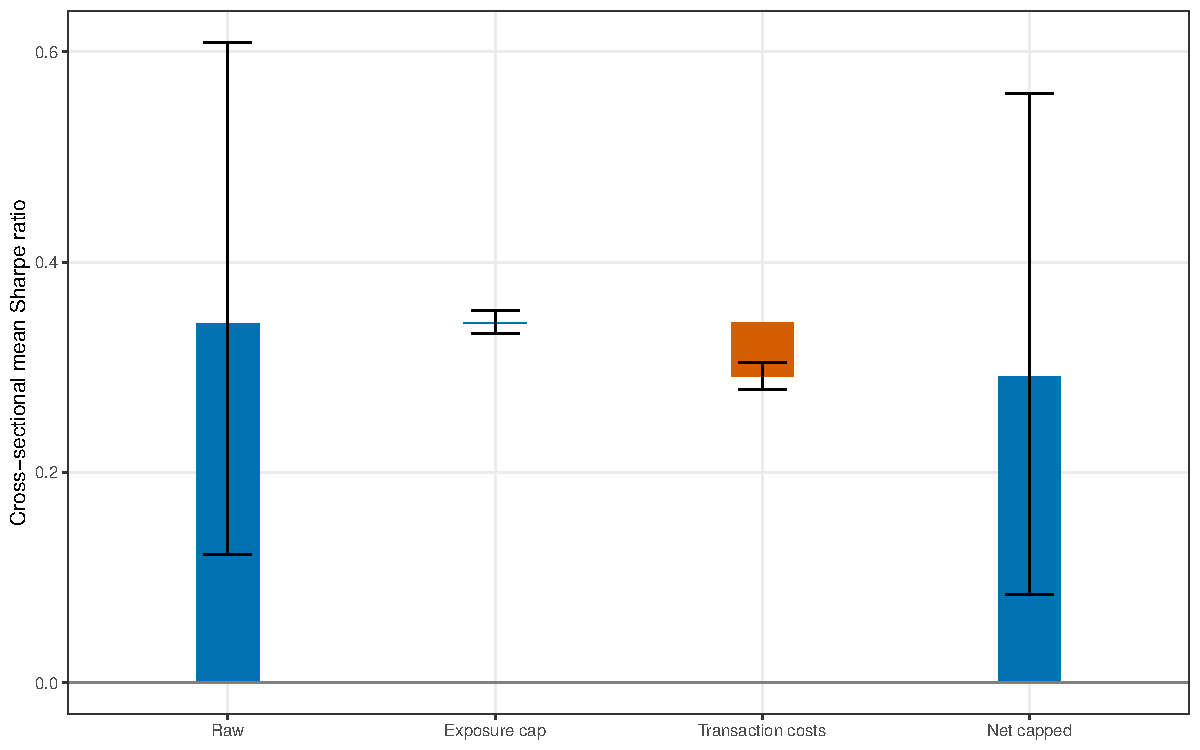
\includegraphics[width=\linewidth,height=0.70\textheight,keepaspectratio]{results_v3/1927/internet_appendix/portfolio_ew_sharpe_waterfall.pdf}
\end{figure}
\begin{figure}[p]
\ContinuedFloat
\centering
\captionsetup{justification=raggedright,labelsep=none,singlelinecheck=false,labelformat=boldlabel}
\caption[]{\footnotesize \textbf{: Decomposition of the equal-weighted forecast strategy's Sharpe ratio across the 153 factors.} The bars show the cross-sectional mean raw Sharpe ratio, the change associated with capping exposure at 1.5, the change associated with transaction costs, and the resulting net capped Sharpe ratio. Error bars report the interquartile range across factors for the raw and final levels and for each intermediate change. Continued.}
\par\smallskip\textbf{Panel B. Short sample}\par\smallskip
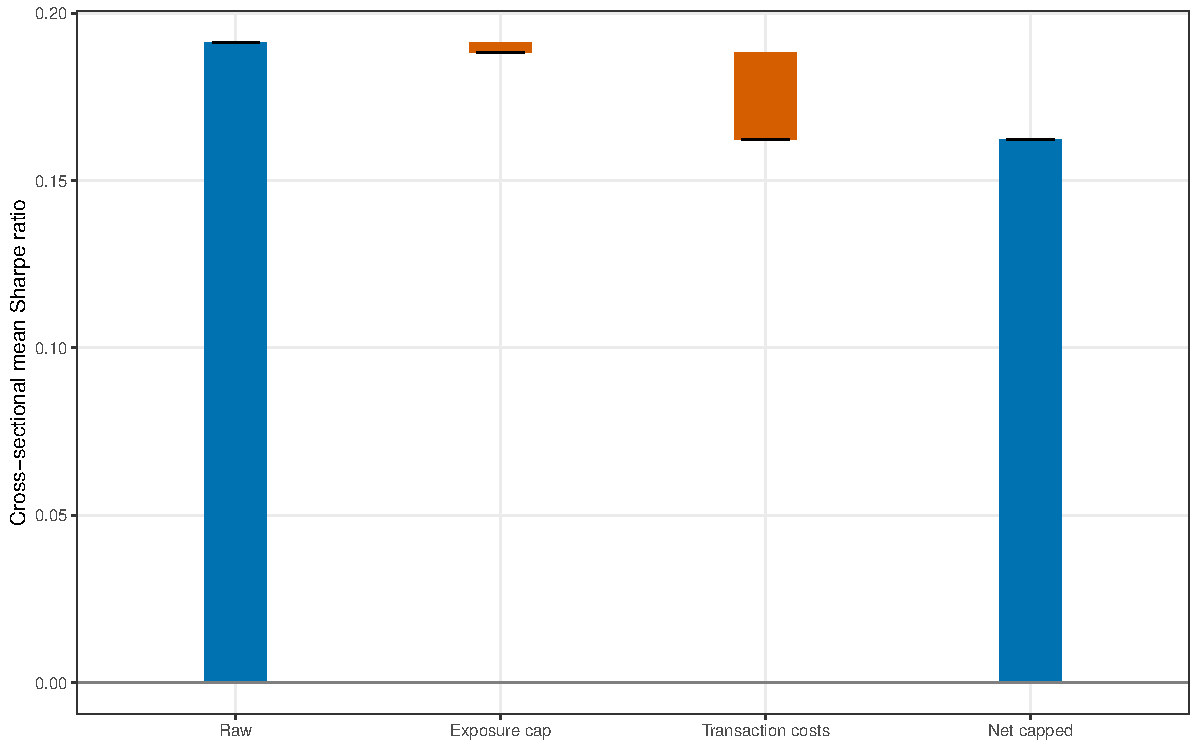
\includegraphics[width=\linewidth,height=0.70\textheight,keepaspectratio]{results_v3/1986/internet_appendix/portfolio_ew_sharpe_waterfall.pdf}
\end{figure}

\begin{landscape}
\begin{table}[p]
\centering\scriptsize
\captionsetup{justification=raggedright,labelsep=none,singlelinecheck=false,labelformat=boldlabel}
\renewcommand{\arraystretch}{0.91}\setlength{\tabcolsep}{4pt}
\caption[]{\footnotesize \textbf{: Implementation statistics for net capped volatility-managed portfolios.} Returns, volatility, CER, drawdowns and costs are percentages. Sharpe and CER use net excess returns. Factor-aggregate performance is computed from monthly aggregate returns. Exposure statistics summarize the underlying positions. Long-sample market strategies span June 1952 to December 2024 and factor aggregates January 1980 to December 2024. Short-sample strategies span July 2011 to December 2024.}
\label{tab:rv-portfolio_implementation}
\resizebox{\ifdim\width>\linewidth\linewidth\else\width\fi}{!}{%
\begin{tabular}{lrrrrrrrrrrr}
\multicolumn{12}{@{}l}{\textit{Panel A. Long sample: Market portfolio, separate estimation}} \\
\hline
Model & Return (\%) & Vol. (\%) & Sharpe & CER (\%) & Vol. ratio & Raw exposure & MDD (\%) & Cost (\%) & Turnover & Max. exposure & Capped (\%) \\
\hline
Unmanaged & 7.530 & 15.086 & 0.499 & 1.841 & 1.000 & 1.000 & -51.570 & 0.001 & 0.001 & 1.000 & 0.000 \\
Random walk & 6.797 & 13.225 & 0.514 & 2.424 & 0.877 & 1.503 & -35.029 & 0.328 & 0.273 & 16.400 & 33.754 \\
HAR & 5.831 & 11.119 & 0.524 & 2.741 & 0.737 & 0.912 & -23.828 & 0.343 & 0.286 & 2.799 & 14.811 \\
HARX & 6.341 & 11.507 & 0.551 & 3.030 & 0.763 & 0.919 & -27.639 & 0.337 & 0.281 & 3.178 & 11.825 \\
EW & 6.385 & 12.153 & 0.525 & 2.692 & 0.806 & 0.968 & -31.160 & 0.315 & 0.262 & 3.222 & 11.596 \\
\hline
\multicolumn{12}{@{}l}{\textit{Panel B. Long sample: Market portfolio, pooled estimation}} \\
\hline
Model & Return (\%) & Vol. (\%) & Sharpe & CER (\%) & Vol. ratio & Raw exposure & MDD (\%) & Cost (\%) & Turnover & Max. exposure & Capped (\%) \\
\hline
Unmanaged & 7.530 & 15.086 & 0.499 & 1.841 & 1.000 & 1.000 & -51.570 & 0.001 & 0.001 & 1.000 & 0.000 \\
Random walk & 6.797 & 13.225 & 0.514 & 2.424 & 0.877 & 1.503 & -35.029 & 0.328 & 0.273 & 16.400 & 33.754 \\
HAR & 6.461 & 12.371 & 0.522 & 2.635 & 0.820 & 0.970 & -30.898 & 0.287 & 0.239 & 2.428 & 13.203 \\
HARX & 6.529 & 12.373 & 0.528 & 2.702 & 0.820 & 0.957 & -33.732 & 0.281 & 0.234 & 2.971 & 12.055 \\
EW & 6.231 & 11.989 & 0.520 & 2.637 & 0.795 & 0.926 & -31.742 & 0.283 & 0.236 & 3.159 & 11.481 \\
\hline
\multicolumn{12}{@{}l}{\textit{Panel C. Long sample: Equal-weighted factor panel}} \\
\hline
Model & Return (\%) & Vol. (\%) & Sharpe & CER (\%) & Vol. ratio & Raw exposure & MDD (\%) & Cost (\%) & Turnover & Max. exposure & Capped (\%) \\
\hline
Unmanaged & 2.602 & 3.623 & 0.718 & 2.274 & 1.000 & 1.000 & -8.844 & 0.000 & 0.000 & 1.000 & 0.000 \\
Random walk & 1.201 & 1.444 & 0.831 & 1.149 & 0.399 & 0.909 & -2.417 & 0.322 & 0.269 & 18.442 & 17.311 \\
HAR & 1.413 & 1.696 & 0.833 & 1.341 & 0.468 & 0.838 & -3.832 & 0.276 & 0.230 & 5.033 & 11.772 \\
HARX & 1.416 & 1.645 & 0.861 & 1.348 & 0.454 & 0.807 & -3.568 & 0.269 & 0.224 & 6.468 & 10.312 \\
EW & 1.520 & 1.651 & 0.920 & 1.452 & 0.456 & 0.854 & -3.472 & 0.259 & 0.216 & 4.938 & 11.383 \\
\hline
\end{tabular}}
\end{table}
\end{landscape}
\begin{landscape}
\begin{table}[p]
\ContinuedFloat
\centering\scriptsize
\captionsetup{justification=raggedright,labelsep=none,singlelinecheck=false,labelformat=boldlabel}
\renewcommand{\arraystretch}{0.91}\setlength{\tabcolsep}{4pt}
\caption[]{\footnotesize \textbf{: Implementation statistics for net capped volatility-managed portfolios. Continued.} Short-sample results. Definitions and conventions follow the preceding panels.}
\resizebox{\ifdim\width>\linewidth\linewidth\else\width\fi}{!}{%
\begin{tabular}{lrrrrrrrrrrr}
\multicolumn{12}{@{}l}{\textit{Panel D. Short sample: Market portfolio, separate estimation}} \\
\hline
Model & Return (\%) & Vol. (\%) & Sharpe & CER (\%) & Vol. ratio & Raw exposure & MDD (\%) & Cost (\%) & Turnover & Max. exposure & Capped (\%) \\
\hline
Unmanaged & 11.527 & 14.985 & 0.769 & 5.913 & 1.000 & 1.000 & -24.982 & 0.007 & 0.006 & 1.000 & 0.000 \\
Random walk & 7.205 & 10.419 & 0.692 & 4.492 & 0.695 & 1.080 & -16.355 & 0.472 & 0.393 & 4.909 & 24.074 \\
HAR & 10.800 & 13.393 & 0.806 & 6.316 & 0.894 & 1.543 & -15.359 & 0.324 & 0.270 & 4.394 & 43.827 \\
HARX & 8.159 & 14.373 & 0.568 & 2.994 & 0.959 & 1.453 & -28.404 & 0.340 & 0.283 & 4.016 & 40.741 \\
EW & 10.346 & 14.916 & 0.694 & 4.784 & 0.995 & 1.517 & -25.610 & 0.254 & 0.211 & 3.291 & 50.617 \\
\hline
\multicolumn{12}{@{}l}{\textit{Panel E. Short sample: Market portfolio, pooled estimation}} \\
\hline
Model & Return (\%) & Vol. (\%) & Sharpe & CER (\%) & Vol. ratio & Raw exposure & MDD (\%) & Cost (\%) & Turnover & Max. exposure & Capped (\%) \\
\hline
Unmanaged & 11.527 & 14.985 & 0.769 & 5.913 & 1.000 & 1.000 & -24.982 & 0.007 & 0.006 & 1.000 & 0.000 \\
Random walk & 7.205 & 10.419 & 0.692 & 4.492 & 0.695 & 1.080 & -16.355 & 0.472 & 0.393 & 4.909 & 24.074 \\
HAR & 11.881 & 14.352 & 0.828 & 6.732 & 0.958 & 1.612 & -16.464 & 0.267 & 0.223 & 4.170 & 45.062 \\
HARX & 10.267 & 14.036 & 0.731 & 5.342 & 0.937 & 1.471 & -19.589 & 0.285 & 0.237 & 3.780 & 40.741 \\
EW & 11.048 & 14.543 & 0.760 & 5.760 & 0.971 & 1.460 & -19.474 & 0.259 & 0.216 & 3.315 & 45.062 \\
\hline
\multicolumn{12}{@{}l}{\textit{Panel F. Short sample: Equal-weighted factor panel}} \\
\hline
Model & Return (\%) & Vol. (\%) & Sharpe & CER (\%) & Vol. ratio & Raw exposure & MDD (\%) & Cost (\%) & Turnover & Max. exposure & Capped (\%) \\
\hline
Unmanaged & 1.288 & 2.686 & 0.480 & 1.108 & 1.001 & 1.000 & -8.844 & 0.007 & 0.006 & 1.000 & 0.000 \\
Random walk & 0.499 & 1.346 & 0.371 & 0.453 & 0.501 & 0.852 & -2.417 & 0.306 & 0.255 & 8.928 & 15.900 \\
HAR & 0.948 & 2.040 & 0.465 & 0.844 & 0.760 & 1.161 & -5.007 & 0.276 & 0.230 & 6.120 & 25.704 \\
HARX & 1.020 & 2.033 & 0.501 & 0.916 & 0.757 & 1.136 & -4.626 & 0.263 & 0.219 & 5.771 & 27.403 \\
EW & 1.062 & 2.031 & 0.523 & 0.959 & 0.756 & 1.132 & -4.498 & 0.240 & 0.200 & 4.406 & 27.080 \\
\hline
\end{tabular}}
\end{table}
\end{landscape}

\begin{landscape}
\begin{table}[p]
\centering\scriptsize
\captionsetup{justification=raggedright,labelsep=none,singlelinecheck=false,labelformat=boldlabel}
\renewcommand{\arraystretch}{0.91}\setlength{\tabcolsep}{4pt}
\caption[]{\footnotesize \textbf{: Economic performance of signed two-sleeve mean-variance portfolios.} Signed two-sleeve MVO is compared with unmanaged-only MVO, which estimates the factor and cash allocation. Total exposure is bounded between minus five and five. Net results deduct factor-exposure costs. Returns, volatility, CER, drawdown and costs are annualized percentages except drawdown, which measures the full evaluation path. Long-sample market strategies span June 1952 to December 2024 and factor aggregates January 1980 to December 2024. Short-sample strategies span July 2011 to December 2024.}
\label{tab:rv-portfolio_performance_cederburg_mvo}
\resizebox{\ifdim\width>\linewidth\linewidth\else\width\fi}{!}{%
\begin{tabular}{lrrrrrrrrr}
\multicolumn{10}{@{}l}{\textit{Panel A. Long sample: Market portfolio, pooled estimation}} \\
\hline
Model & Return (\%) & Vol. (\%) & Gross SR & Net SR & CER (\%) & MDD (\%) & Turnover & Cost (\%) & Mean exposure \\
\hline
Unmanaged-only MVO & 7.571 & 15.619 & 0.486 & 0.485 & 1.472 & -47.696 & 0.017 & 0.021 & 1.034 \\
Random walk & 5.078 & 11.210 & 0.491 & 0.453 & 1.936 & -31.042 & 0.355 & 0.426 & 0.823 \\
HAR & 5.372 & 14.768 & 0.378 & 0.364 & -0.080 & -47.551 & 0.179 & 0.214 & 0.884 \\
HARX & 4.891 & 14.892 & 0.343 & 0.328 & -0.654 & -47.766 & 0.182 & 0.219 & 0.869 \\
EW forecast ensemble & 5.051 & 14.943 & 0.355 & 0.338 & -0.531 & -47.546 & 0.212 & 0.254 & 0.868 \\
\hline
\multicolumn{10}{@{}l}{\textit{Panel B. Long sample: Equal-weighted 153-factor aggregate}} \\
\hline
Model & Return (\%) & Vol. (\%) & Gross SR & Net SR & CER (\%) & MDD (\%) & Turnover & Cost (\%) & Mean exposure \\
\hline
Unmanaged-only MVO & 4.882 & 3.410 & 1.437 & 1.432 & 4.591 & -5.885 & 0.017 & 0.020 & 1.330 \\
Random walk & 4.184 & 2.709 & 1.689 & 1.544 & 4.001 & -3.535 & 0.336 & 0.403 & 1.323 \\
HAR & 4.337 & 2.908 & 1.616 & 1.491 & 4.125 & -3.484 & 0.309 & 0.371 & 1.319 \\
HARX & 4.187 & 2.833 & 1.605 & 1.478 & 3.987 & -3.616 & 0.306 & 0.368 & 1.283 \\
EW forecast ensemble & 4.181 & 2.968 & 1.540 & 1.409 & 3.961 & -5.085 & 0.334 & 0.401 & 1.296 \\
\hline
\multicolumn{10}{@{}l}{\textit{Panel C. Long sample: Market portfolio, separate estimation}} \\
\hline
Model & Return (\%) & Vol. (\%) & Gross SR & Net SR & CER (\%) & MDD (\%) & Turnover & Cost (\%) & Mean exposure \\
\hline
Unmanaged-only MVO & 7.571 & 15.619 & 0.486 & 0.485 & 1.472 & -47.696 & 0.017 & 0.021 & 1.034 \\
Random walk & 5.078 & 11.210 & 0.491 & 0.453 & 1.936 & -31.042 & 0.355 & 0.426 & 0.823 \\
HAR & 5.839 & 15.464 & 0.398 & 0.378 & -0.140 & -48.819 & 0.267 & 0.321 & 0.911 \\
HARX & 5.791 & 14.983 & 0.406 & 0.387 & 0.179 & -49.314 & 0.247 & 0.296 & 0.983 \\
EW forecast ensemble & 6.127 & 16.266 & 0.394 & 0.377 & -0.487 & -53.644 & 0.240 & 0.288 & 1.024 \\
\hline
\end{tabular}}
\end{table}
\end{landscape}
\begin{landscape}
\begin{table}[p]
\ContinuedFloat
\centering\scriptsize
\captionsetup{justification=raggedright,labelsep=none,singlelinecheck=false,labelformat=boldlabel}
\renewcommand{\arraystretch}{0.91}\setlength{\tabcolsep}{4pt}
\caption[]{\footnotesize \textbf{: Economic performance of signed two-sleeve mean-variance portfolios. Continued.} Short-sample results. Definitions and conventions follow the preceding panels.}
\resizebox{\ifdim\width>\linewidth\linewidth\else\width\fi}{!}{%
\begin{tabular}{lrrrrrrrrr}
\multicolumn{10}{@{}l}{\textit{Panel D. Short sample: Market portfolio, pooled estimation}} \\
\hline
Model & Return (\%) & Vol. (\%) & Gross SR & Net SR & CER (\%) & MDD (\%) & Turnover & Cost (\%) & Mean exposure \\
\hline
Unmanaged-only MVO & 5.959 & 9.491 & 0.631 & 0.628 & 3.707 & -19.406 & 0.025 & 0.029 & 0.600 \\
Random walk & 5.402 & 9.235 & 0.629 & 0.585 & 3.270 & -20.672 & 0.331 & 0.398 & 0.662 \\
HAR & 11.952 & 21.063 & 0.609 & 0.567 & 0.862 & -45.853 & 0.722 & 0.867 & 1.555 \\
HARX & 10.999 & 20.383 & 0.583 & 0.540 & 0.612 & -44.226 & 0.748 & 0.898 & 1.553 \\
EW forecast ensemble & 10.351 & 19.241 & 0.577 & 0.538 & 1.095 & -41.303 & 0.633 & 0.760 & 1.486 \\
\hline
\multicolumn{10}{@{}l}{\textit{Panel E. Short sample: Equal-weighted 153-factor aggregate}} \\
\hline
Model & Return (\%) & Vol. (\%) & Gross SR & Net SR & CER (\%) & MDD (\%) & Turnover & Cost (\%) & Mean exposure \\
\hline
Unmanaged-only MVO & 0.761 & 1.624 & 0.522 & 0.469 & 0.695 & -3.388 & 0.071 & 0.085 & 0.499 \\
Random walk & 1.373 & 1.615 & 1.070 & 0.850 & 1.308 & -3.535 & 0.294 & 0.353 & 1.106 \\
HAR & 1.533 & 2.414 & 0.972 & 0.635 & 1.388 & -3.190 & 0.690 & 0.828 & 0.731 \\
HARX & 1.633 & 2.757 & 0.887 & 0.592 & 1.443 & -5.486 & 0.680 & 0.816 & 0.698 \\
EW forecast ensemble & 1.817 & 2.837 & 0.906 & 0.641 & 1.616 & -5.036 & 0.626 & 0.751 & 0.748 \\
\hline
\multicolumn{10}{@{}l}{\textit{Panel F. Short sample: Market portfolio, separate estimation}} \\
\hline
Model & Return (\%) & Vol. (\%) & Gross SR & Net SR & CER (\%) & MDD (\%) & Turnover & Cost (\%) & Mean exposure \\
\hline
Unmanaged-only MVO & 5.959 & 9.491 & 0.631 & 0.628 & 3.707 & -19.406 & 0.025 & 0.029 & 0.600 \\
Random walk & 5.402 & 9.235 & 0.629 & 0.585 & 3.270 & -20.672 & 0.331 & 0.398 & 0.662 \\
HAR & 12.378 & 21.367 & 0.624 & 0.579 & 0.964 & -45.899 & 0.814 & 0.977 & 1.546 \\
HARX & 6.447 & 14.690 & 0.471 & 0.439 & 1.052 & -26.084 & 0.393 & 0.471 & 1.086 \\
EW forecast ensemble & 8.203 & 17.167 & 0.511 & 0.478 & 0.836 & -33.972 & 0.480 & 0.576 & 1.312 \\
\hline
\end{tabular}}
\end{table}
\end{landscape}

\begin{table}[p]
\centering\scriptsize
\captionsetup{justification=raggedright,labelsep=none,singlelinecheck=false,labelformat=boldlabel}
\renewcommand{\arraystretch}{0.91}\setlength{\tabcolsep}{4pt}
\caption[]{\footnotesize \textbf{: Spanning regressions for net single-factor portfolios relative to unmanaged exposure.} The dependent variable is the net managed excess return and the regressor is unmanaged excess return. Alpha is annualized. Newey-West statistics use lag one. Spanning is an ex-post opportunity-set diagnostic. Long-sample market strategies span June 1952 to December 2024 and factor aggregates January 1980 to December 2024. Short-sample strategies span July 2011 to December 2024.}
\label{tab:rv-portfolio_spanning_single_factor}
\resizebox{\ifdim\width>\linewidth\linewidth\else\width\fi}{!}{%
\begin{tabular}{lrrrrrrr}
\multicolumn{8}{@{}l}{\textit{Panel A. Long sample: Fixed 50/50 combination}} \\
\hline
Scope & Exposure & Alpha (\%) & t(alpha) & p-value & Beta & R2 & Appraisal ratio \\
\hline
153-factor aggregate & Capped & 0.295 & 3.586 & 0.000 & 0.683 & 0.951 & 0.526 \\
Pooled market & Capped & 0.569 & 1.451 & 0.147 & 0.852 & 0.945 & 0.183 \\
\hline
\multicolumn{8}{@{}l}{\textit{Panel B. Long sample: Moreira--Muir management}} \\
\hline
Scope & Exposure & Alpha (\%) & t(alpha) & p-value & Beta & R2 & Appraisal ratio \\
\hline
153-factor aggregate & Capped & 0.588 & 3.946 & 0.000 & 0.358 & 0.618 & 0.576 \\
153-factor aggregate & Raw & 0.590 & 3.586 & 0.000 & 0.366 & 0.582 & 0.526 \\
Pooled market & Capped & 1.006 & 1.359 & 0.174 & 0.694 & 0.762 & 0.172 \\
Pooled market & Raw & 1.138 & 1.451 & 0.147 & 0.703 & 0.744 & 0.183 \\
\hline
\multicolumn{8}{@{}l}{\textit{Panel C. Short sample: Fixed 50/50 combination}} \\
\hline
Scope & Exposure & Alpha (\%) & t(alpha) & p-value & Beta & R2 & Appraisal ratio \\
\hline
153-factor aggregate & Capped & 0.086 & 0.496 & 0.620 & 0.845 & 0.923 & 0.132 \\
Pooled market & Capped & 0.921 & 0.663 & 0.507 & 0.978 & 0.891 & 0.180 \\
\hline
\multicolumn{8}{@{}l}{\textit{Panel D. Short sample: Moreira--Muir management}} \\
\hline
Scope & Exposure & Alpha (\%) & t(alpha) & p-value & Beta & R2 & Appraisal ratio \\
\hline
153-factor aggregate & Capped & 0.223 & 0.810 & 0.418 & 0.651 & 0.741 & 0.217 \\
153-factor aggregate & Raw & 0.172 & 0.496 & 0.620 & 0.690 & 0.668 & 0.132 \\
Pooled market & Capped & 1.282 & 0.710 & 0.478 & 0.847 & 0.762 & 0.181 \\
Pooled market & Raw & 1.841 & 0.663 & 0.507 & 0.957 & 0.662 & 0.180 \\
\hline
\end{tabular}}
\end{table}

\begin{table}[p]
\centering\scriptsize
\captionsetup{justification=raggedright,labelsep=none,singlelinecheck=false,labelformat=boldlabel}
\renewcommand{\arraystretch}{0.91}\setlength{\tabcolsep}{4pt}
\caption[]{\footnotesize \textbf{: Paired mean excess return comparisons.} Each row compares the EW forecast ensemble with the stated benchmark, using net returns. Intervals are pointwise 95 percent percentile intervals from 10,000 paired stationary-bootstrap draws with expected block length five months. One-sided p-values use centered bootstrap errors. Holm and Benjamini-Hochberg (BH) adjustments use the same prespecified family across Sharpe, mean and CER, separately within each sample. BH controls the false discovery rate under its dependence assumptions. Inference is conditional on fitted forecasts. Long-sample market strategies span June 1952 to December 2024 and factor aggregates January 1980 to December 2024. Short-sample strategies span July 2011 to December 2024.}
\label{tab:rv-portfolio_inference_single_factor_primary_mean_ann_1}
\resizebox{\ifdim\width>\linewidth\linewidth\else\width\fi}{!}{%
\begin{tabular}{lrrrrr}
\multicolumn{6}{@{}l}{\textit{Panel A. Long sample: 50/50 single-factor combination, 153-factor aggregate}} \\
\hline
Benchmark & Exposure & Difference (pp) & 95\% interval & p-value & Holm p-value \\
\hline
Unmanaged & Capped & -0.530 & [-1.032, -0.126] & 0.979 & 1.000 \\
RW & Capped & 0.092 & [-0.022, 0.211] & 0.066 & 1.000 \\
HAR & Capped & 0.057 & [0.018, 0.095] & 0.002 & 0.140 \\
HARX & Capped & 0.059 & [0.027, 0.088] & 0.000 & 0.010 \\
Unmanaged & Raw & -0.530 & [-1.032, -0.126] & 0.979 & 1.000 \\
RW & Raw & 0.093 & [-0.023, 0.212] & 0.065 & 1.000 \\
HAR & Raw & 0.057 & [0.018, 0.095] & 0.002 & 0.140 \\
HARX & Raw & 0.059 & [0.027, 0.088] & 0.000 & 0.010 \\
\hline
\multicolumn{6}{@{}l}{\textit{Panel B. Long sample: MM management, 153-factor aggregate}} \\
\hline
Benchmark & Exposure & Difference (pp) & 95\% interval & p-value & Holm p-value \\
\hline
Unmanaged & Capped & -1.082 & [-2.082, -0.287] & 0.982 & 1.000 \\
RW & Capped & 0.319 & [0.158, 0.507] & 0.001 & 0.074 \\
HAR & Capped & 0.107 & [0.035, 0.175] & 0.001 & 0.054 \\
HARX & Capped & 0.104 & [0.040, 0.159] & 0.000 & 0.010 \\
Unmanaged & Raw & -1.060 & [-2.065, -0.252] & 0.979 & 1.000 \\
RW & Raw & 0.186 & [-0.046, 0.425] & 0.065 & 1.000 \\
HAR & Raw & 0.114 & [0.036, 0.190] & 0.002 & 0.140 \\
HARX & Raw & 0.119 & [0.053, 0.176] & 0.000 & 0.010 \\
\hline
\multicolumn{6}{@{}l}{\textit{Panel C. Long sample: 50/50 single-factor combination, Pooled market}} \\
\hline
Benchmark & Exposure & Difference (pp) & 95\% interval & p-value & Holm p-value \\
\hline
Unmanaged & Capped & -0.549 & [-1.474, 0.382] & 0.884 & 1.000 \\
RW & Capped & -1.543 & [-3.025, -0.145] & 0.980 & 1.000 \\
HAR & Capped & -0.137 & [-0.352, 0.078] & 0.894 & 1.000 \\
HARX & Capped & -0.130 & [-0.279, 0.014] & 0.960 & 1.000 \\
Unmanaged & Raw & -0.549 & [-1.474, 0.382] & 0.884 & 1.000 \\
RW & Raw & -1.633 & [-3.151, -0.201] & 0.983 & 1.000 \\
HAR & Raw & -0.137 & [-0.352, 0.078] & 0.894 & 1.000 \\
HARX & Raw & -0.130 & [-0.279, 0.014] & 0.960 & 1.000 \\
\hline
\multicolumn{6}{@{}l}{\textit{Panel D. Long sample: MM management, Pooled market}} \\
\hline
Benchmark & Exposure & Difference (pp) & 95\% interval & p-value & Holm p-value \\
\hline
Unmanaged & Capped & -1.300 & [-3.071, 0.487] & 0.925 & 1.000 \\
RW & Capped & -0.566 & [-1.280, 0.134] & 0.940 & 1.000 \\
HAR & Capped & -0.231 & [-0.600, 0.148] & 0.887 & 1.000 \\
HARX & Capped & -0.298 & [-0.546, -0.047] & 0.990 & 1.000 \\
Unmanaged & Raw & -1.097 & [-2.949, 0.764] & 0.884 & 1.000 \\
RW & Raw & -3.266 & [-6.303, -0.402] & 0.983 & 1.000 \\
HAR & Raw & -0.274 & [-0.704, 0.157] & 0.894 & 1.000 \\
HARX & Raw & -0.260 & [-0.558, 0.028] & 0.960 & 1.000 \\
\hline
\end{tabular}}
\end{table}
\begin{table}[p]
\ContinuedFloat
\centering\scriptsize
\captionsetup{justification=raggedright,labelsep=none,singlelinecheck=false,labelformat=boldlabel}
\renewcommand{\arraystretch}{0.91}\setlength{\tabcolsep}{4pt}
\caption[]{\footnotesize \textbf{: Paired mean excess return comparisons. Continued.} Short-sample results. Definitions and conventions follow the preceding panels.}
\resizebox{\ifdim\width>\linewidth\linewidth\else\width\fi}{!}{%
\begin{tabular}{lrrrrr}
\multicolumn{6}{@{}l}{\textit{Panel E. Short sample: 50/50 single-factor combination, 153-factor aggregate}} \\
\hline
Benchmark & Exposure & Difference (pp) & 95\% interval & p-value & Holm p-value \\
\hline
Unmanaged & Capped & -0.114 & [-0.604, 0.348] & 0.698 & 1.000 \\
RW & Capped & 0.255 & [-0.011, 0.538] & 0.038 & 1.000 \\
HAR & Capped & 0.035 & [-0.077, 0.148] & 0.269 & 1.000 \\
HARX & Capped & 0.065 & [-0.000, 0.129] & 0.022 & 1.000 \\
Unmanaged & Raw & -0.114 & [-0.604, 0.348] & 0.698 & 1.000 \\
RW & Raw & 0.255 & [-0.011, 0.538] & 0.038 & 1.000 \\
HAR & Raw & 0.035 & [-0.077, 0.148] & 0.269 & 1.000 \\
HARX & Raw & 0.065 & [-0.000, 0.129] & 0.022 & 1.000 \\
\hline
\multicolumn{6}{@{}l}{\textit{Panel F. Short sample: 50/50 single-factor combination, Pooled market}} \\
\hline
Benchmark & Exposure & Difference (pp) & 95\% interval & p-value & Holm p-value \\
\hline
Unmanaged & Capped & 0.671 & [-2.409, 3.657] & 0.338 & 1.000 \\
RW & Capped & 2.502 & [-0.060, 5.051] & 0.027 & 1.000 \\
HAR & Capped & -0.567 & [-2.263, 1.154] & 0.741 & 1.000 \\
HARX & Capped & -0.033 & [-0.810, 0.709] & 0.537 & 1.000 \\
Unmanaged & Raw & 0.671 & [-2.409, 3.657] & 0.338 & 1.000 \\
RW & Raw & 2.502 & [-0.060, 5.051] & 0.027 & 1.000 \\
HAR & Raw & -0.567 & [-2.263, 1.154] & 0.741 & 1.000 \\
HARX & Raw & -0.033 & [-0.810, 0.709] & 0.537 & 1.000 \\
\hline
\multicolumn{6}{@{}l}{\textit{Panel G. Short sample: MM management, 153-factor aggregate}} \\
\hline
Benchmark & Exposure & Difference (pp) & 95\% interval & p-value & Holm p-value \\
\hline
Unmanaged & Capped & -0.226 & [-1.164, 0.649] & 0.707 & 1.000 \\
RW & Capped & 0.563 & [0.074, 1.089] & 0.018 & 1.000 \\
HAR & Capped & 0.113 & [-0.068, 0.287] & 0.104 & 1.000 \\
HARX & Capped & 0.042 & [-0.043, 0.122] & 0.161 & 1.000 \\
Unmanaged & Raw & -0.228 & [-1.209, 0.696] & 0.698 & 1.000 \\
RW & Raw & 0.509 & [-0.023, 1.076] & 0.038 & 1.000 \\
HAR & Raw & 0.069 & [-0.154, 0.296] & 0.269 & 1.000 \\
HARX & Raw & 0.130 & [-0.000, 0.258] & 0.022 & 1.000 \\
\hline
\multicolumn{6}{@{}l}{\textit{Panel H. Short sample: MM management, Pooled market}} \\
\hline
Benchmark & Exposure & Difference (pp) & 95\% interval & p-value & Holm p-value \\
\hline
Unmanaged & Capped & -0.479 & [-5.025, 3.469] & 0.603 & 1.000 \\
RW & Capped & 3.843 & [0.491, 7.222] & 0.012 & 1.000 \\
HAR & Capped & -0.833 & [-2.302, 0.528] & 0.868 & 1.000 \\
HARX & Capped & 0.781 & [-0.023, 1.617] & 0.033 & 1.000 \\
Unmanaged & Raw & 1.342 & [-4.818, 7.315] & 0.338 & 1.000 \\
RW & Raw & 5.004 & [-0.119, 10.101] & 0.027 & 1.000 \\
HAR & Raw & -1.135 & [-4.527, 2.307] & 0.741 & 1.000 \\
HARX & Raw & -0.066 & [-1.620, 1.417] & 0.537 & 1.000 \\
\hline
\end{tabular}}
\end{table}



\end{appendices}

\end{document}
